%==================================================================
% Ini adalah bab 4
% Silahkan edit sesuai kebutuhan, baik menambah atau mengurangi \section, \subsection
%==================================================================

\chapter[HASIL DAN PEMBAHASAN]{\\ HASIL DAN PEMBAHASAN}

\section{Fungsi \textit{Benchmark}}
Fungsi-fungsi yang disajikan berikut ini merupakan bagian dari kumpulan fungsi yang tersedia CECO.\ Fungsi-fungsi tersebut dirancang untuk digunakan dalam proses \textit{benchmarking} dan pengujian performa berbagai algoritma optimasi. Pada bagian selanjutnya, fungsi-fungsi ini akan digunakan sebagai fungsi evaluasi untuk mengukur efektivitas dan efisiensi algoritma yang diuji dalam menyelesaikan berbagai permasalahan optimasi.
\subsection{Fungsi CEC}
\vspace*{-4.5em}
\begin{flalign*}
  &D: \text{dimensi}&&\\
  &\mathrm{x}=[x_1, x_2, \ldots, x_D]: \text{input}&&\\
  &\mathrm{o}=[o_1, o_2, \ldots, o_D]: \text{shift}&&\\
  &R: \text{Matriks rotasi}&&\\
  &\mathrm{z}=R\times (\mathrm{x}-\mathrm{o}): \text{Matriks rotasi}&&\\
  &f_{\text{bias}}: \text{bias}&&
\end{flalign*}

\subsubsection{Ackley}
\noindent Properti:
\begin{packed_item}
  \item multimodal
  \item non-separable
  \item non-convex
\end{packed_item}
\begin{figure}[H]
	\centering
	\begin{subfigure}[b]{0.4\textwidth}
		\centering
		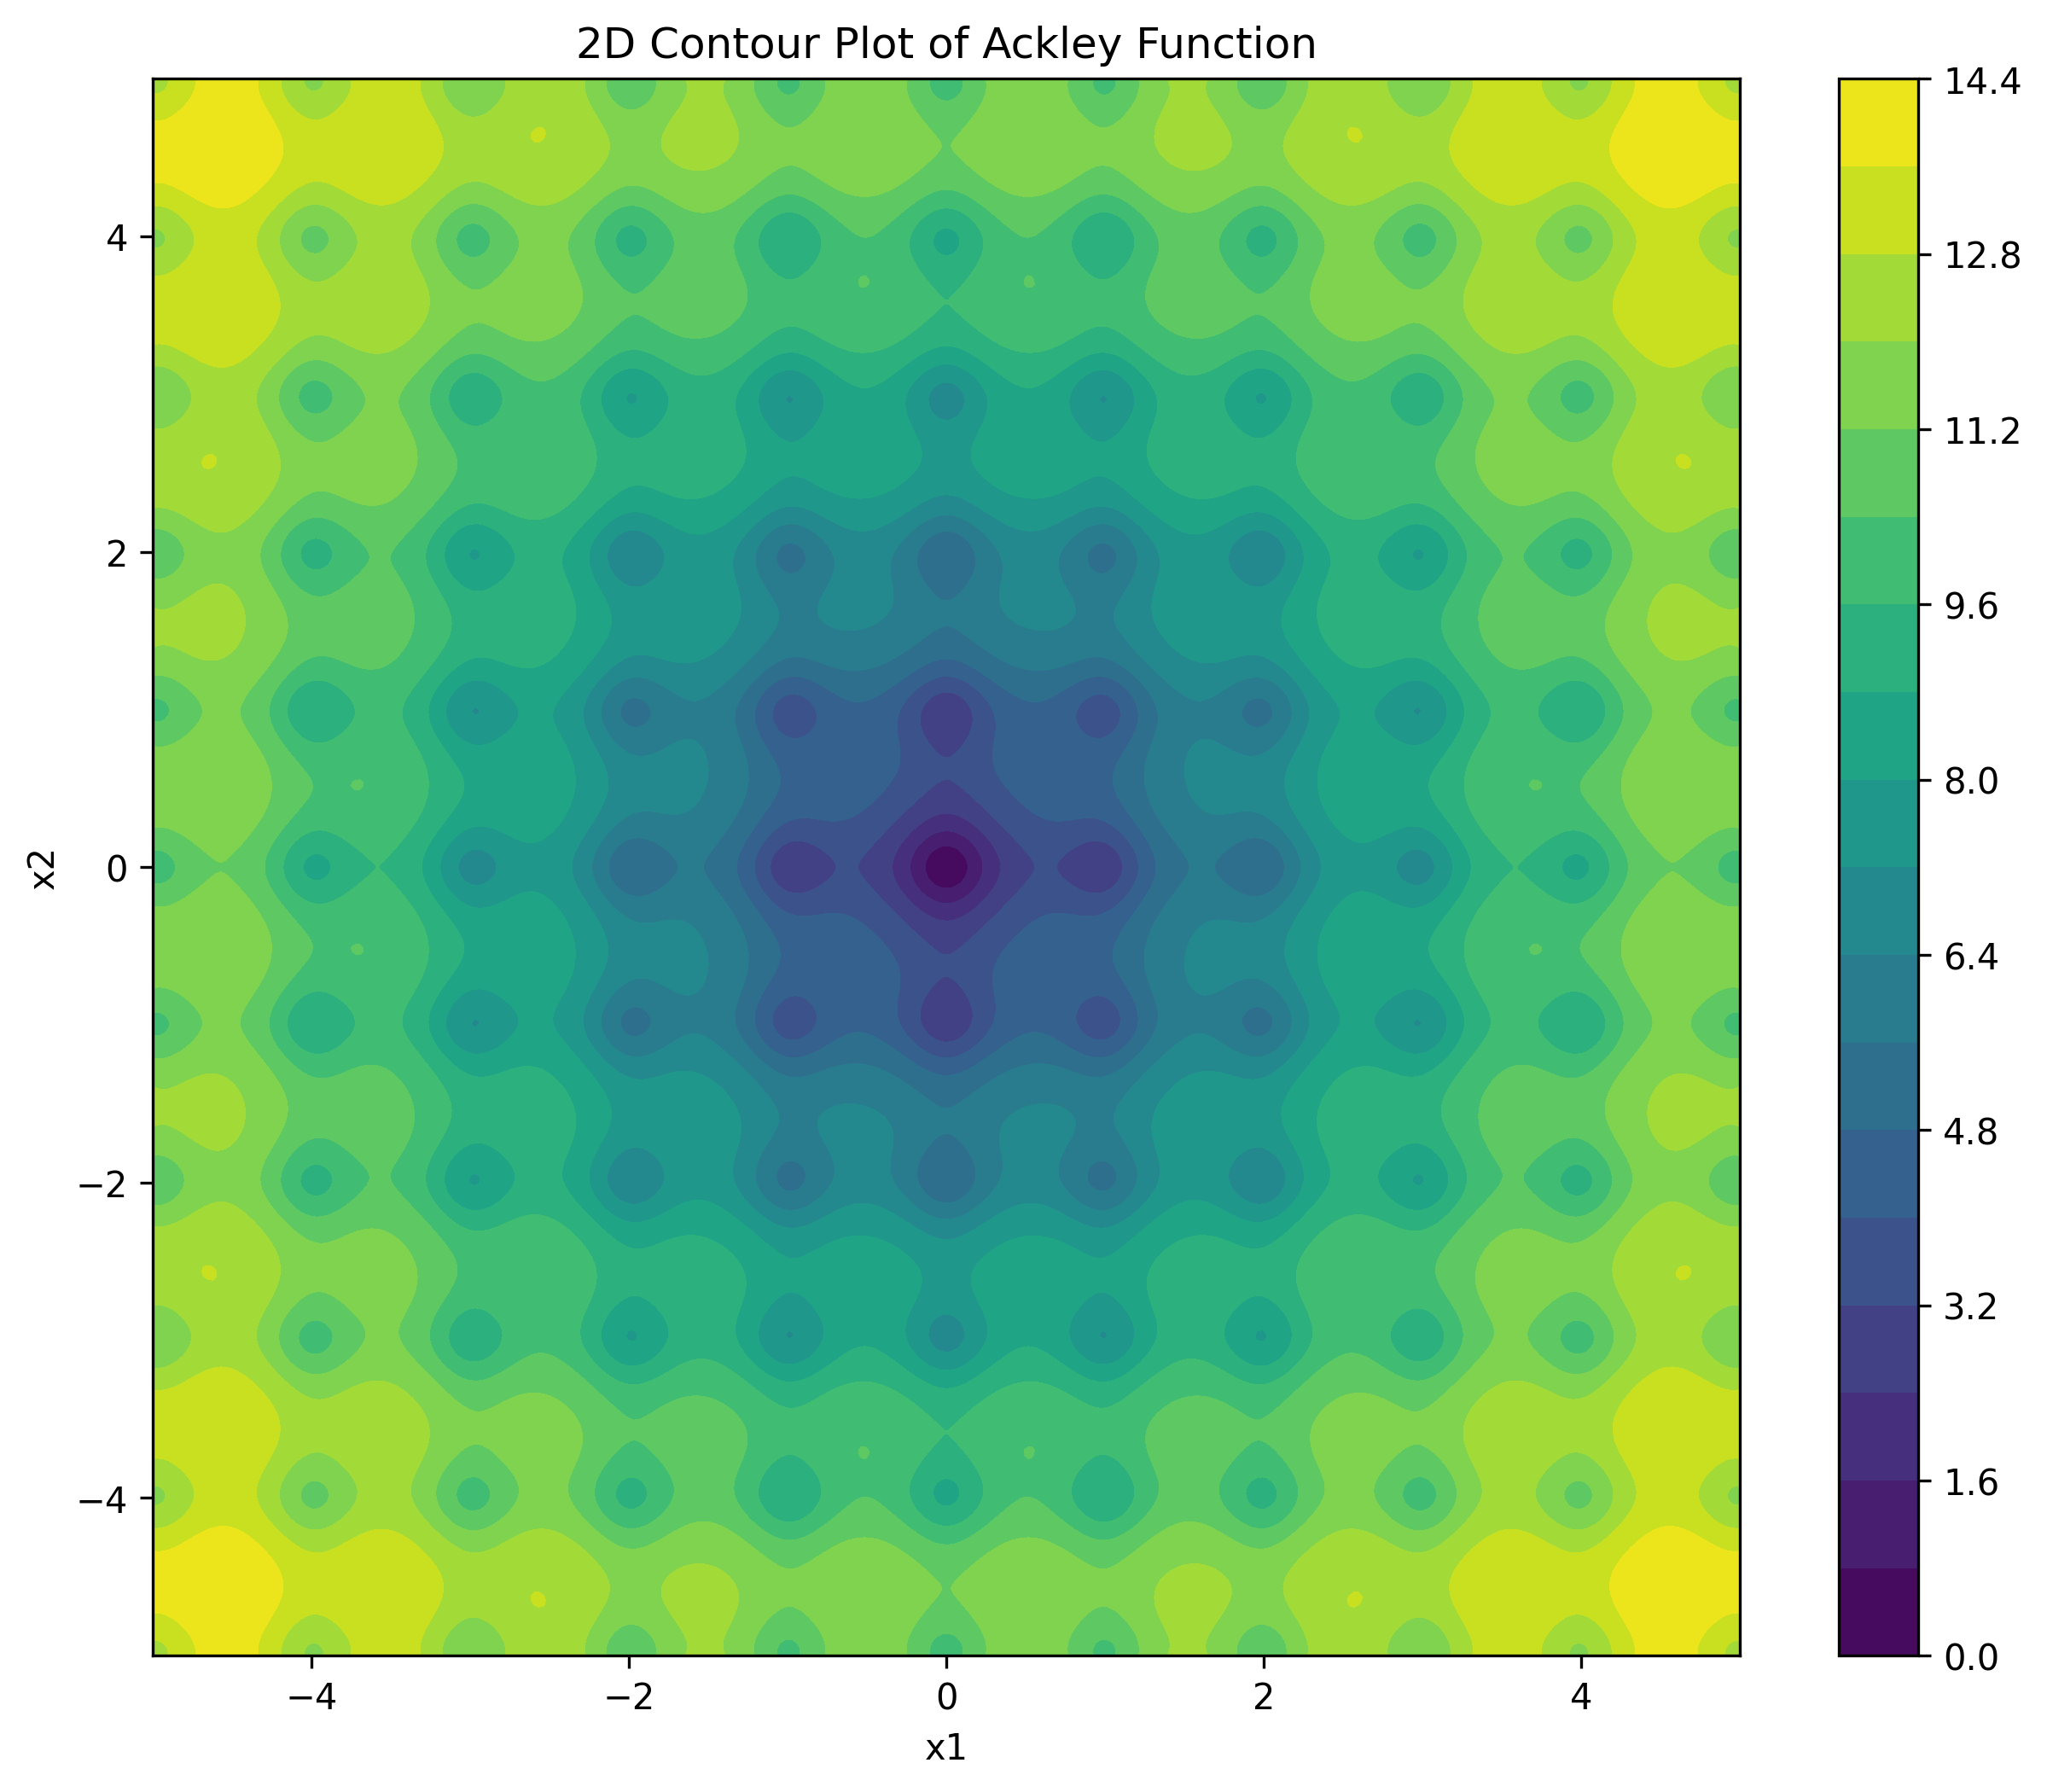
\includegraphics[width=\linewidth]{cec/ackley_2d.png}
		\caption{Dimensi 2}
		\label{fig:ackley-2d}
	\end{subfigure}
	\hfill
	\begin{subfigure}[b]{0.4\textwidth}
		\centering
		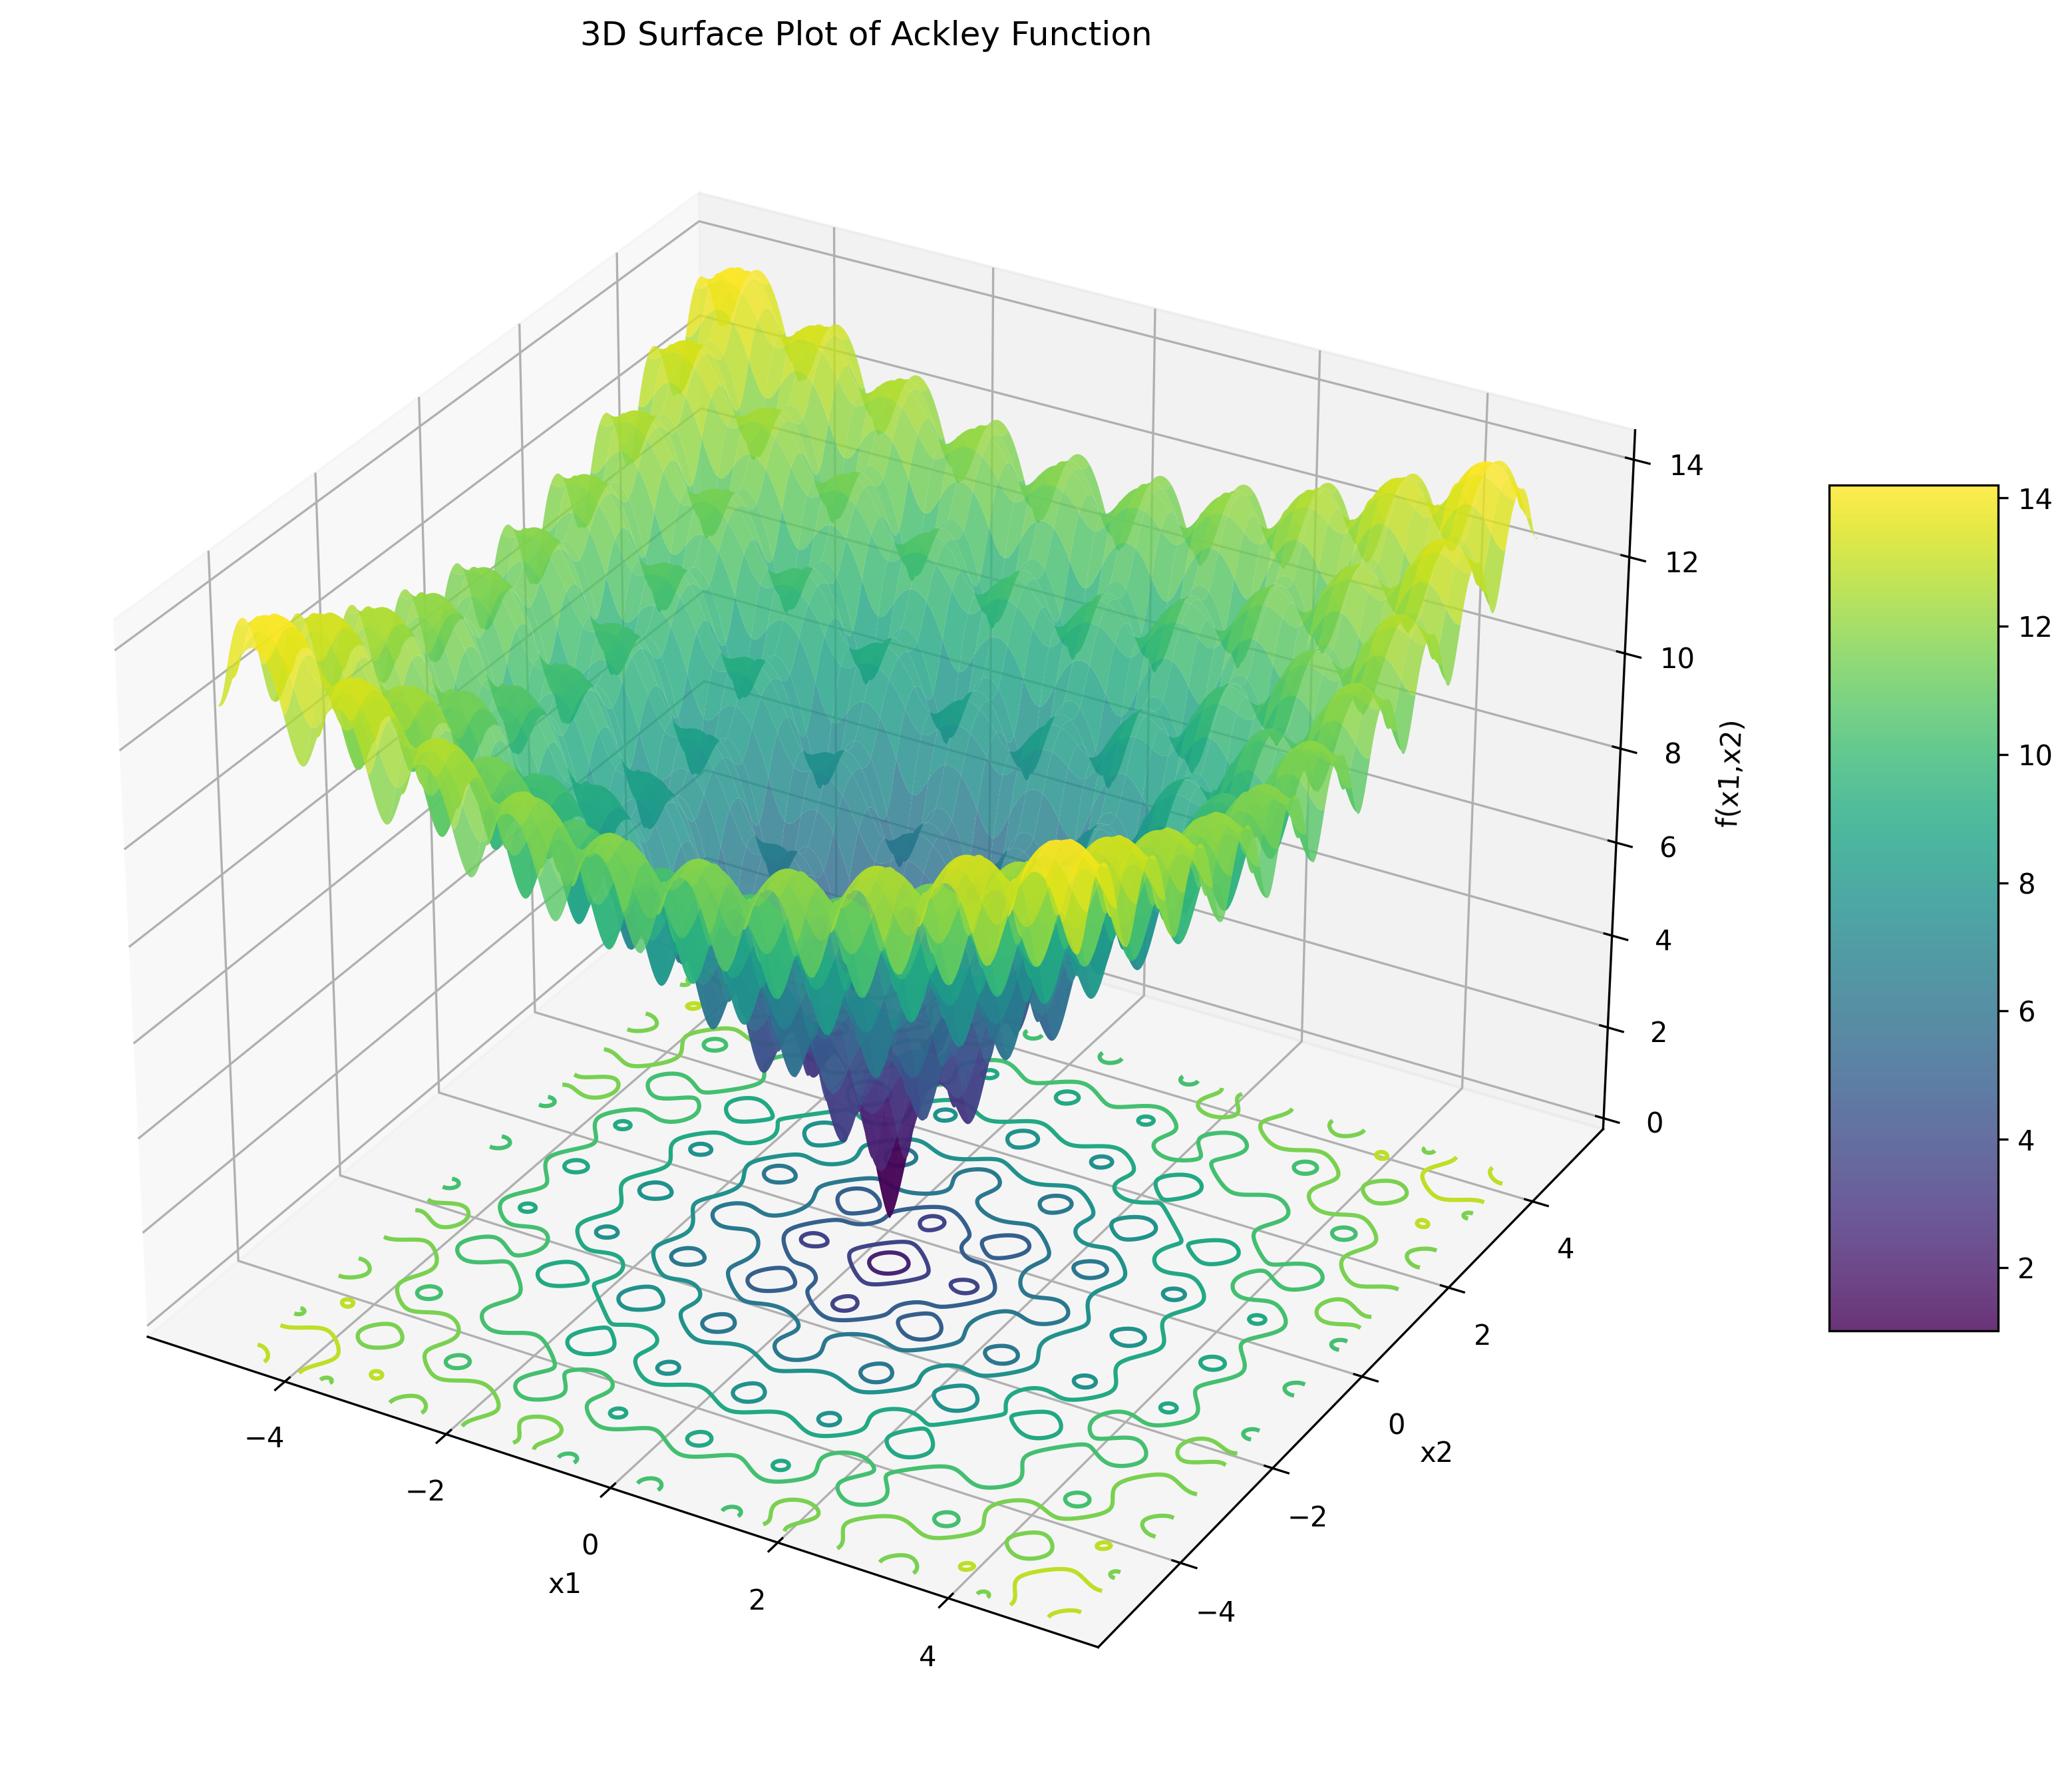
\includegraphics[width=\linewidth]{cec/ackley_3d.png}
		\caption{Dimensi 3}
		\label{fig:ackley-3d}
	\end{subfigure}
	\caption{Tampilan grafik fungsi Ackley pada dimensi dua (\cref{fig:ackley-2d}) dan tiga (\cref{fig:ackley-3d})}
	\label{fig:ackley}
\end{figure}
\begin{flalign*}
  f_{\text{Ackley}}(\mathrm{x})=-20\exp\left(-0.2\sqrt{\frac{1}{D}\sum_{i=1}^{D}z_i^2} \right)-\exp\left( \frac{1}{D}\sum_{i=1}^{D}\cos\left(2\pi z_i \right) \right) + 20 + e +f_{\text{bias}}&&
\end{flalign*}

\subsubsection{Bent Cigar}
\noindent Properti:
\begin{packed_item}
  \item unimodal
  \item non-separable
  \item convex
\end{packed_item}
\begin{figure}[H]
	\centering
	\begin{subfigure}[b]{0.4\textwidth}
		\centering
		\includegraphics[width=\linewidth]{cec/bent_cigar_2d.png}
		\caption{Dimensi 2}
		\label{fig:bentcigar-2d}
	\end{subfigure}
	\hfill
	\begin{subfigure}[b]{0.4\textwidth}
		\centering
		\includegraphics[width=\linewidth]{cec/bent_cigar_3d.png}
		\caption{Dimensi 3}
		\label{fig:bentcigar-3d}
	\end{subfigure}
	\caption{Tampilan grafik fungsi Bent Cigar pada dimensi dua (\cref{fig:bentcigar-2d}) dan tiga (\cref{fig:bentcigar-3d})}
	\label{fig:bentcigar}
\end{figure}
\begin{flalign*}
  f_{\text{Bent cigar}}(\mathrm{x})=z_1^2+10^6\sum_{i=2}^{D}z_i^2+f_{\text{bias}}&&
\end{flalign*}

\subsubsection{Different Power}
\noindent Properti:
\begin{packed_item}
  \item unimodal
  \item separable
  \item convex
\end{packed_item}
\begin{figure}[H]
	\centering
	\begin{subfigure}[b]{0.4\textwidth}
		\centering
		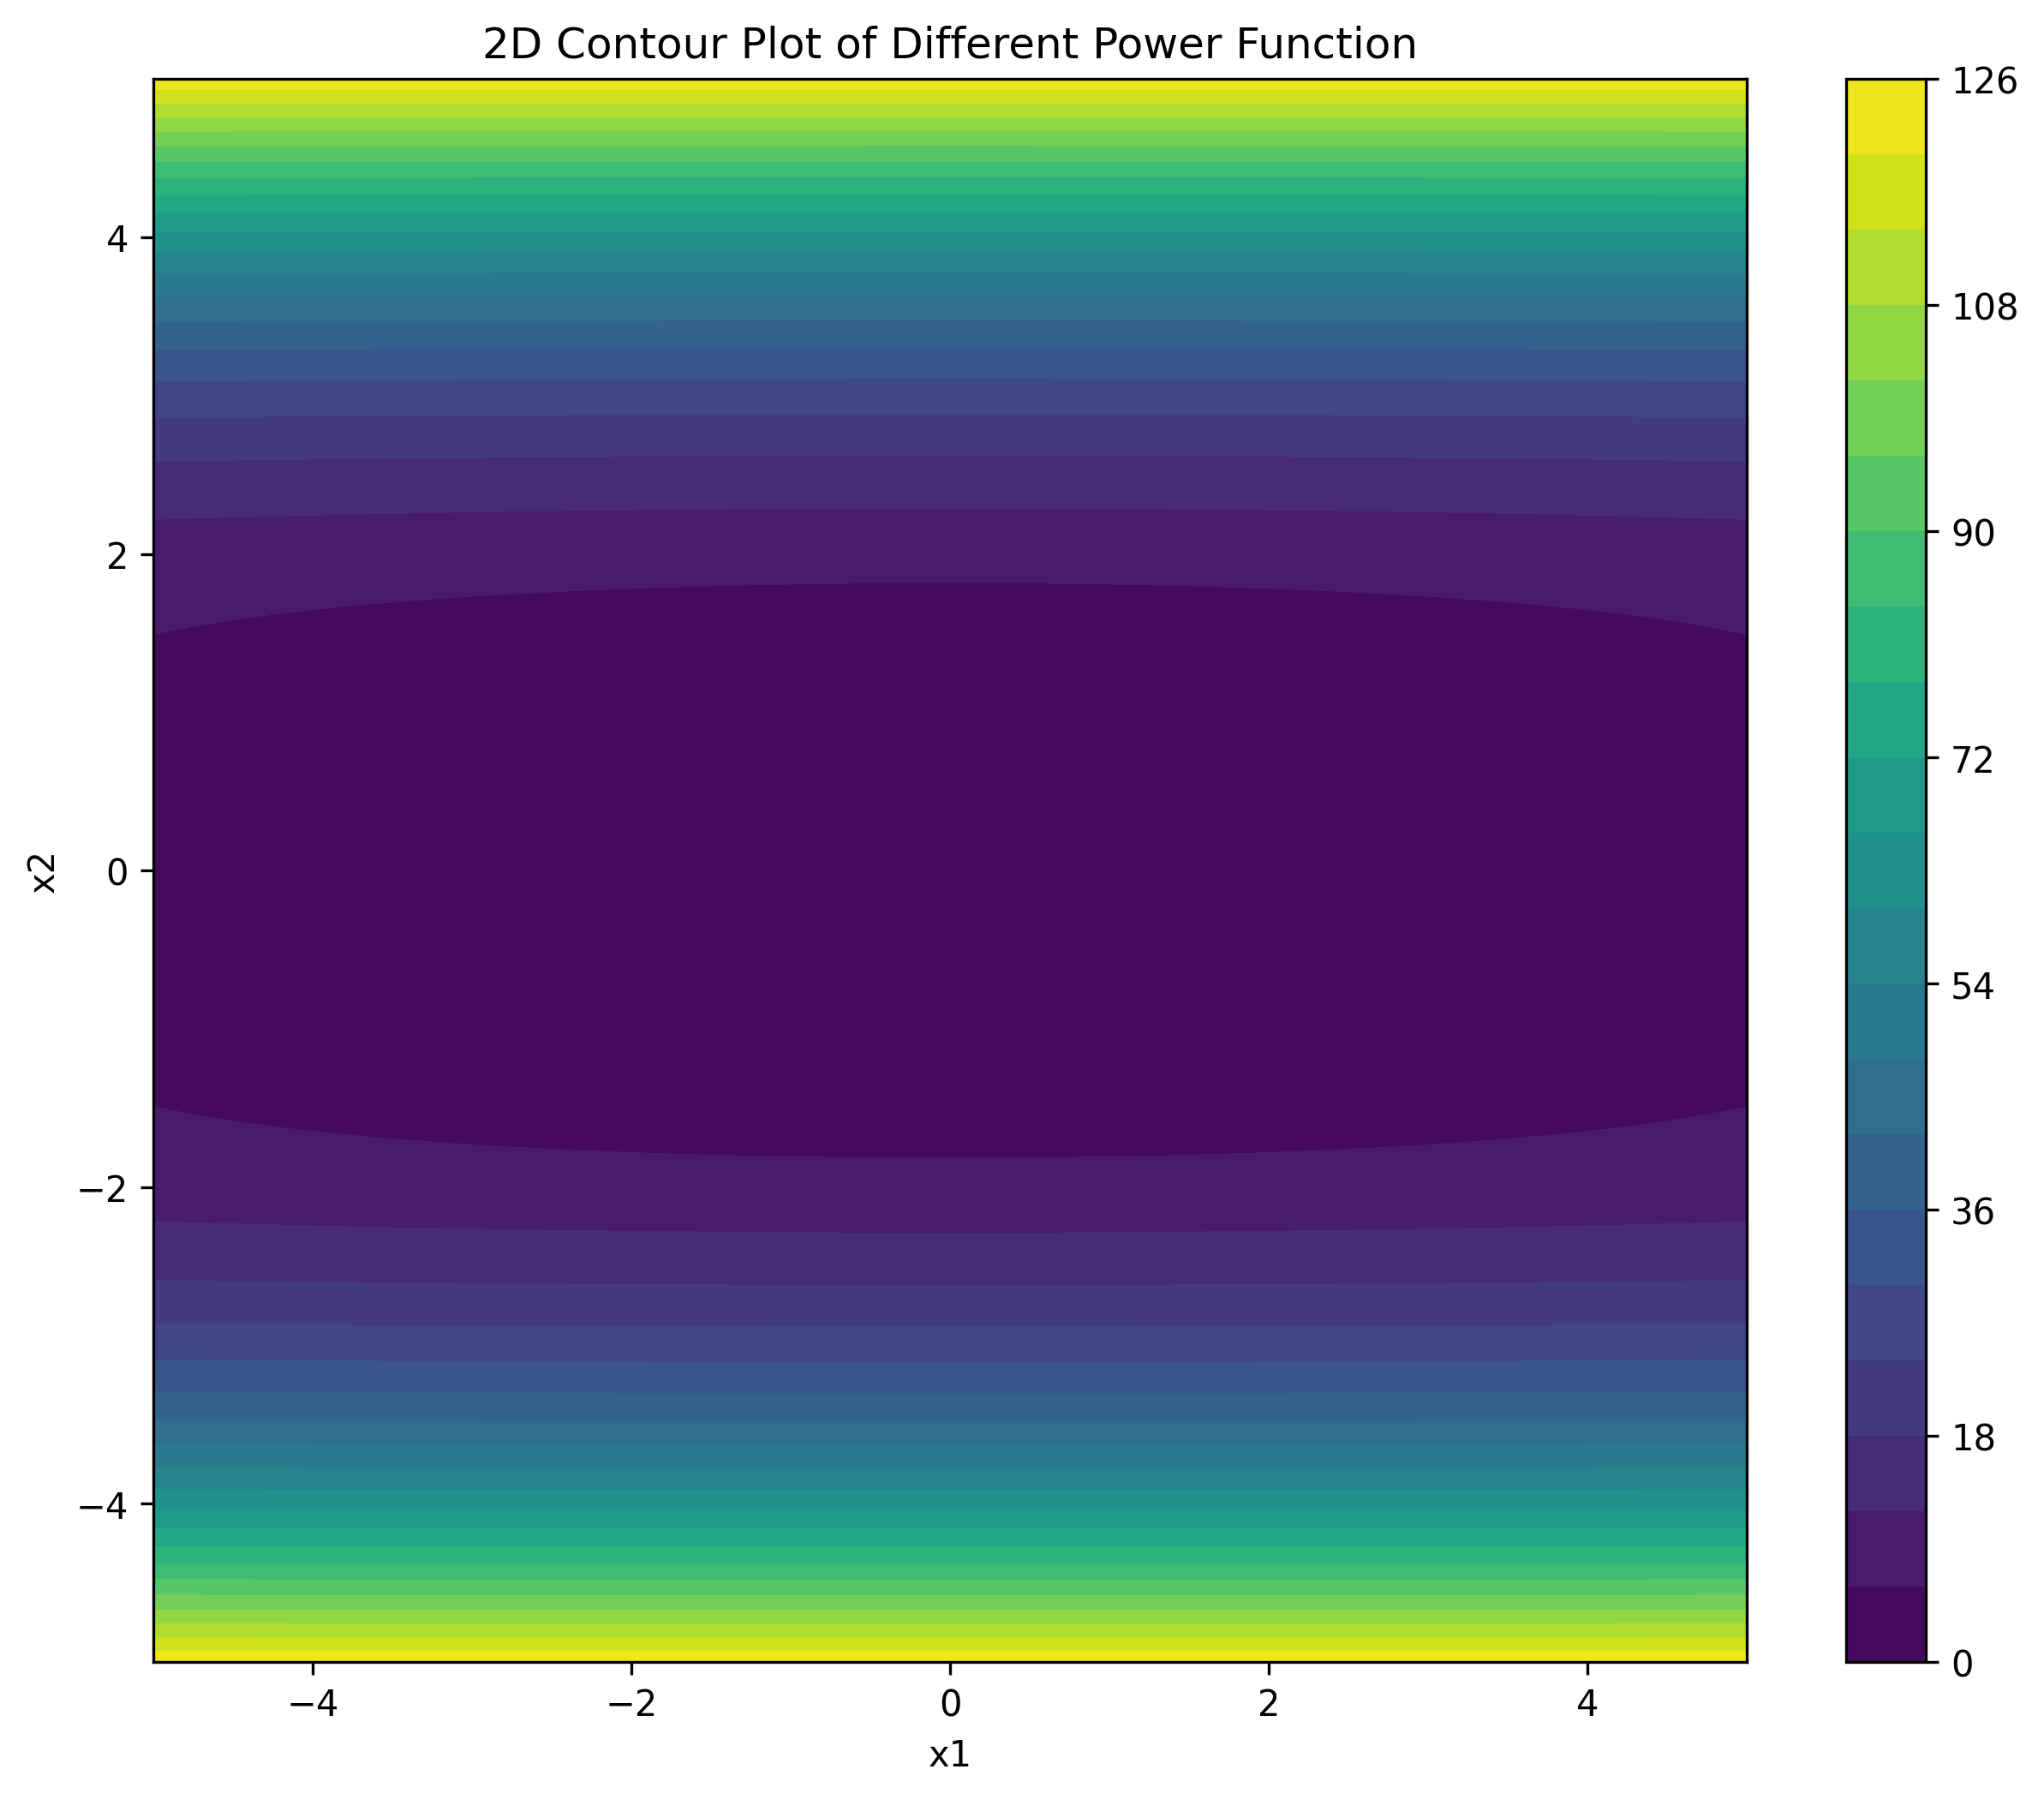
\includegraphics[width=\linewidth]{cec/different_power_2d.png}
		\caption{Dimensi 2}
		\label{fig:diffpower-2d}
	\end{subfigure}
	\hfill
	\begin{subfigure}[b]{0.4\textwidth}
		\centering
		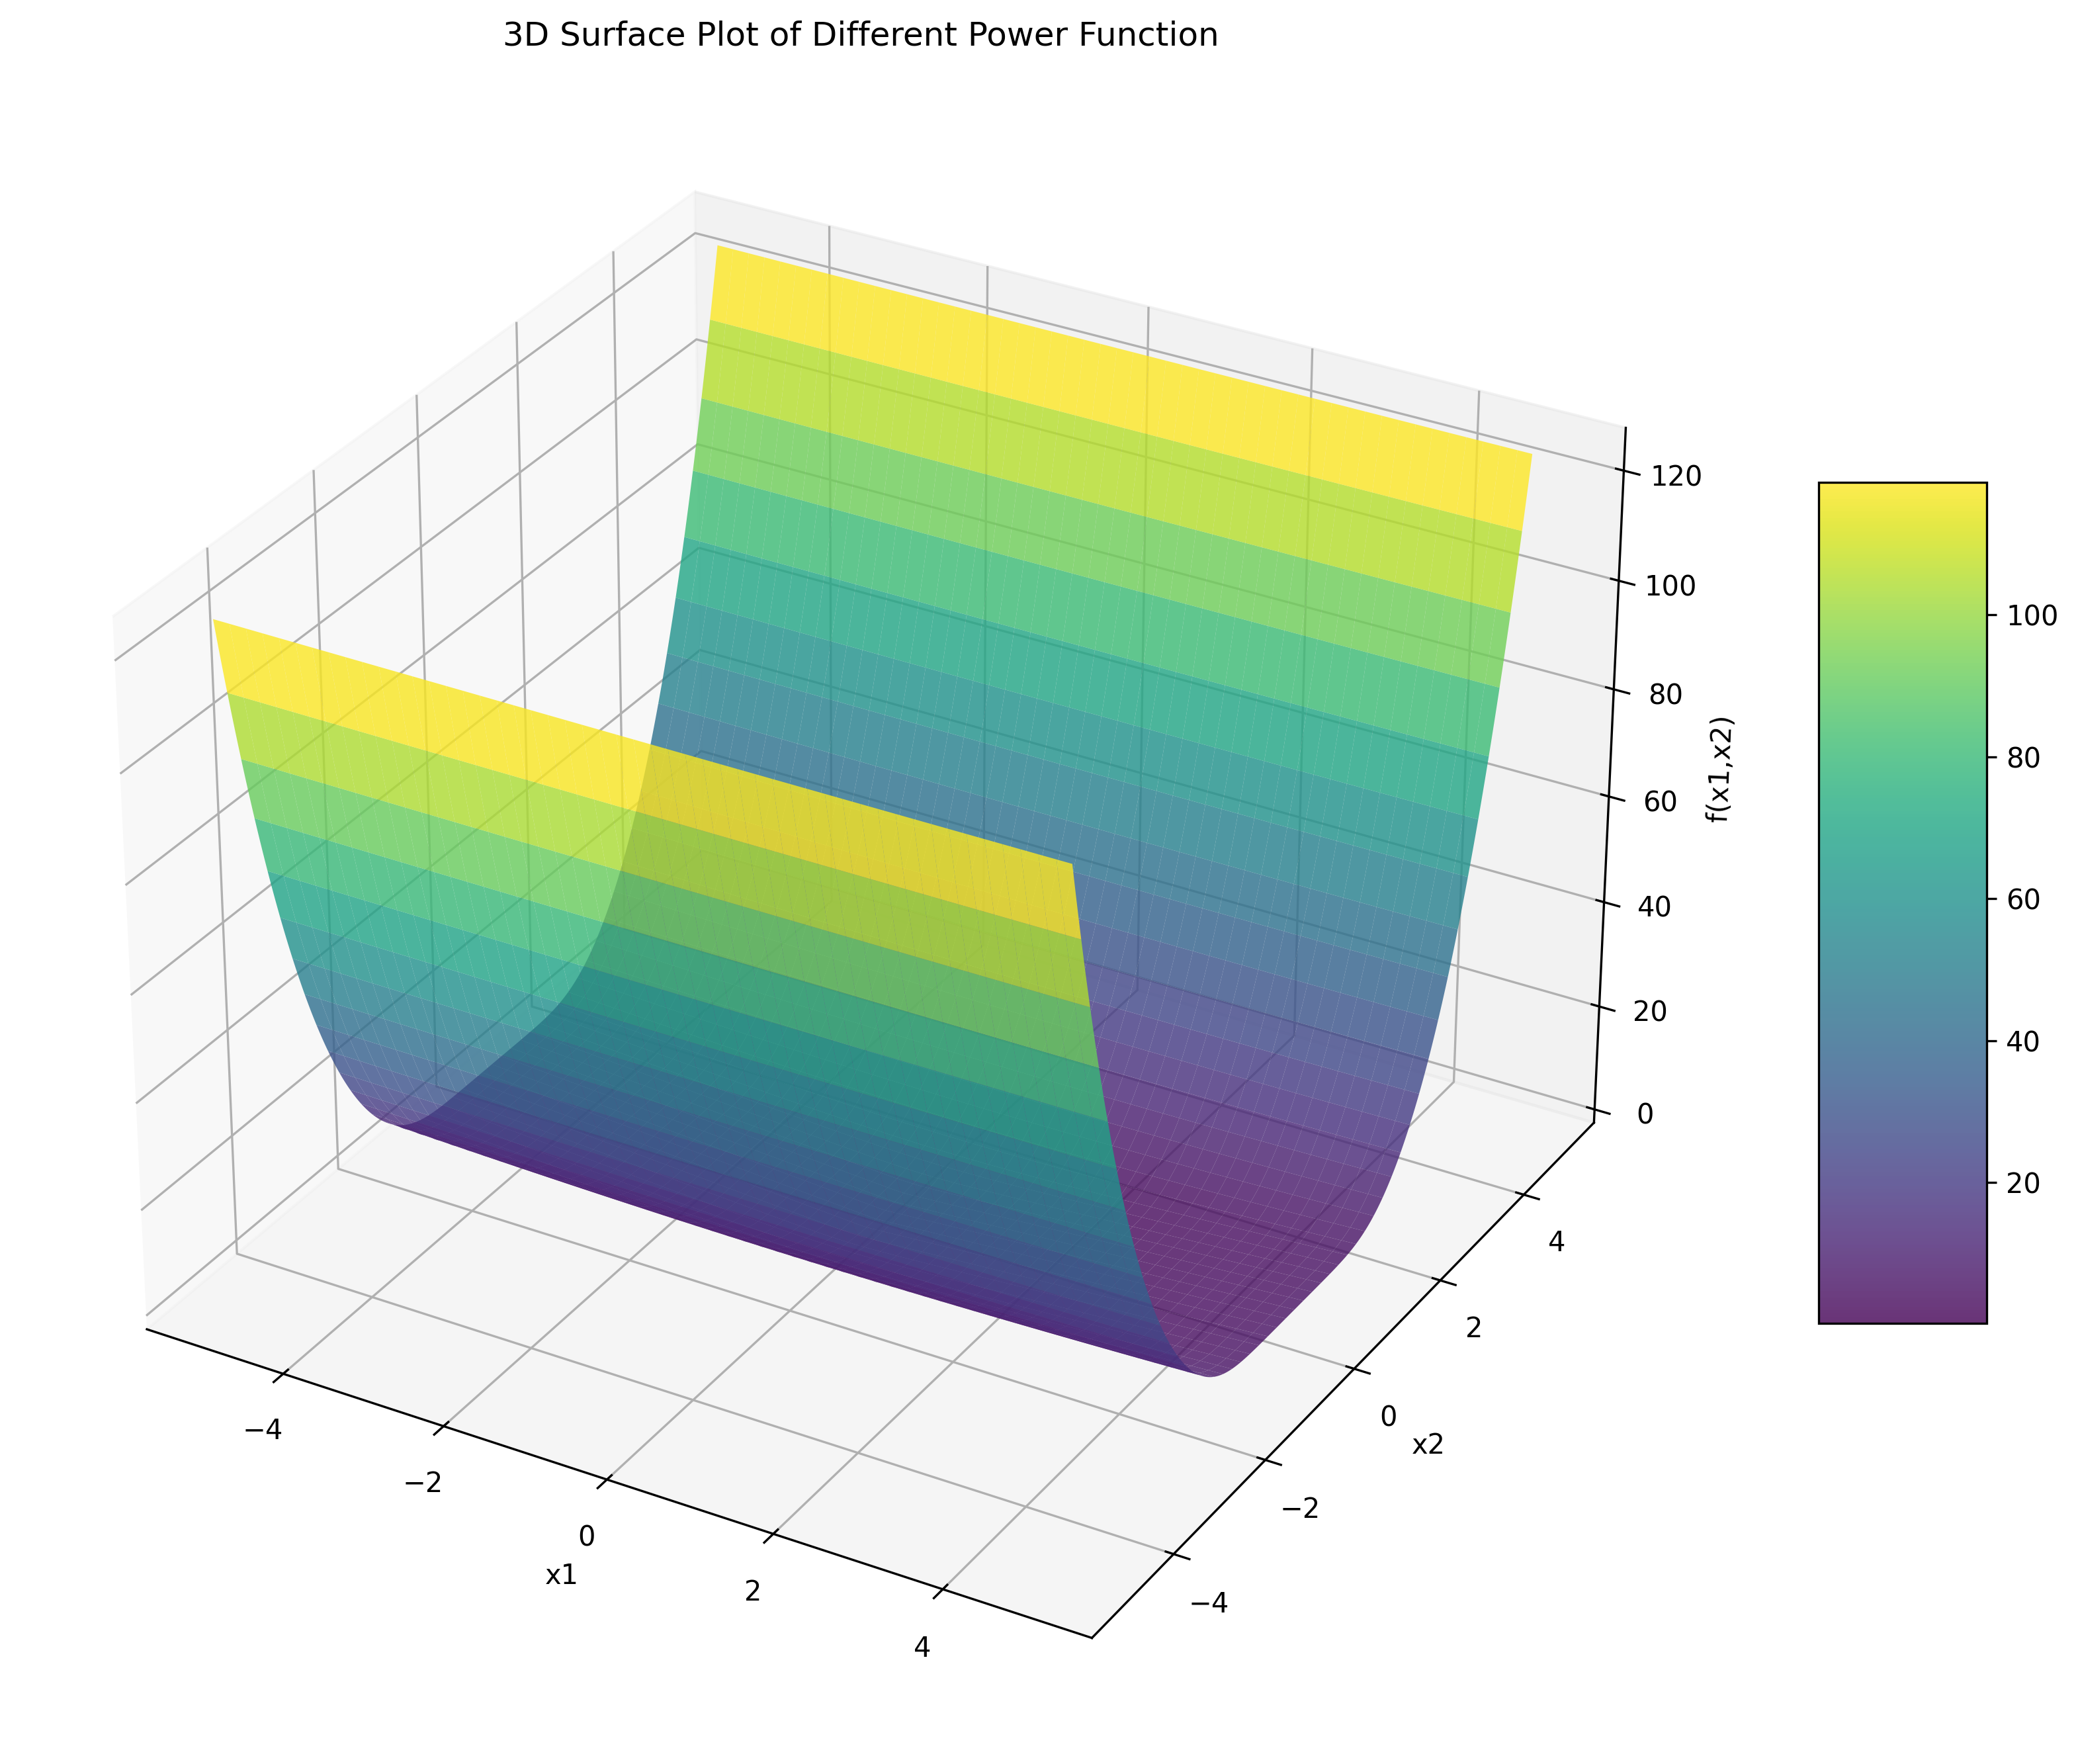
\includegraphics[width=\linewidth]{cec/different_power_3d.png}
		\caption{Dimensi 3}
		\label{fig:diffpower-3d}
	\end{subfigure}
	\caption{Tampilan grafik fungsi Different Power pada dimensi dua (\cref{fig:diffpower-2d}) dan tiga (\cref{fig:diffpower-3d})}
	\label{fig:diffpower}
\end{figure}
\begin{flalign*}
  f_{\text{Different power}}(\mathrm{x})=\sqrt{\sum_{i=1}^{D}\left| z_i \right|^{2+4\frac{i-1}{D-1}} }+f_{\text{bias}}&&
\end{flalign*}

\subsubsection{Discus}
\noindent Properti:
\begin{packed_item}
  \item unimodal
  \item non-separable
  \item convex
\end{packed_item}
\begin{figure}[H]
	\centering
	\begin{subfigure}[b]{0.4\textwidth}
		\centering
		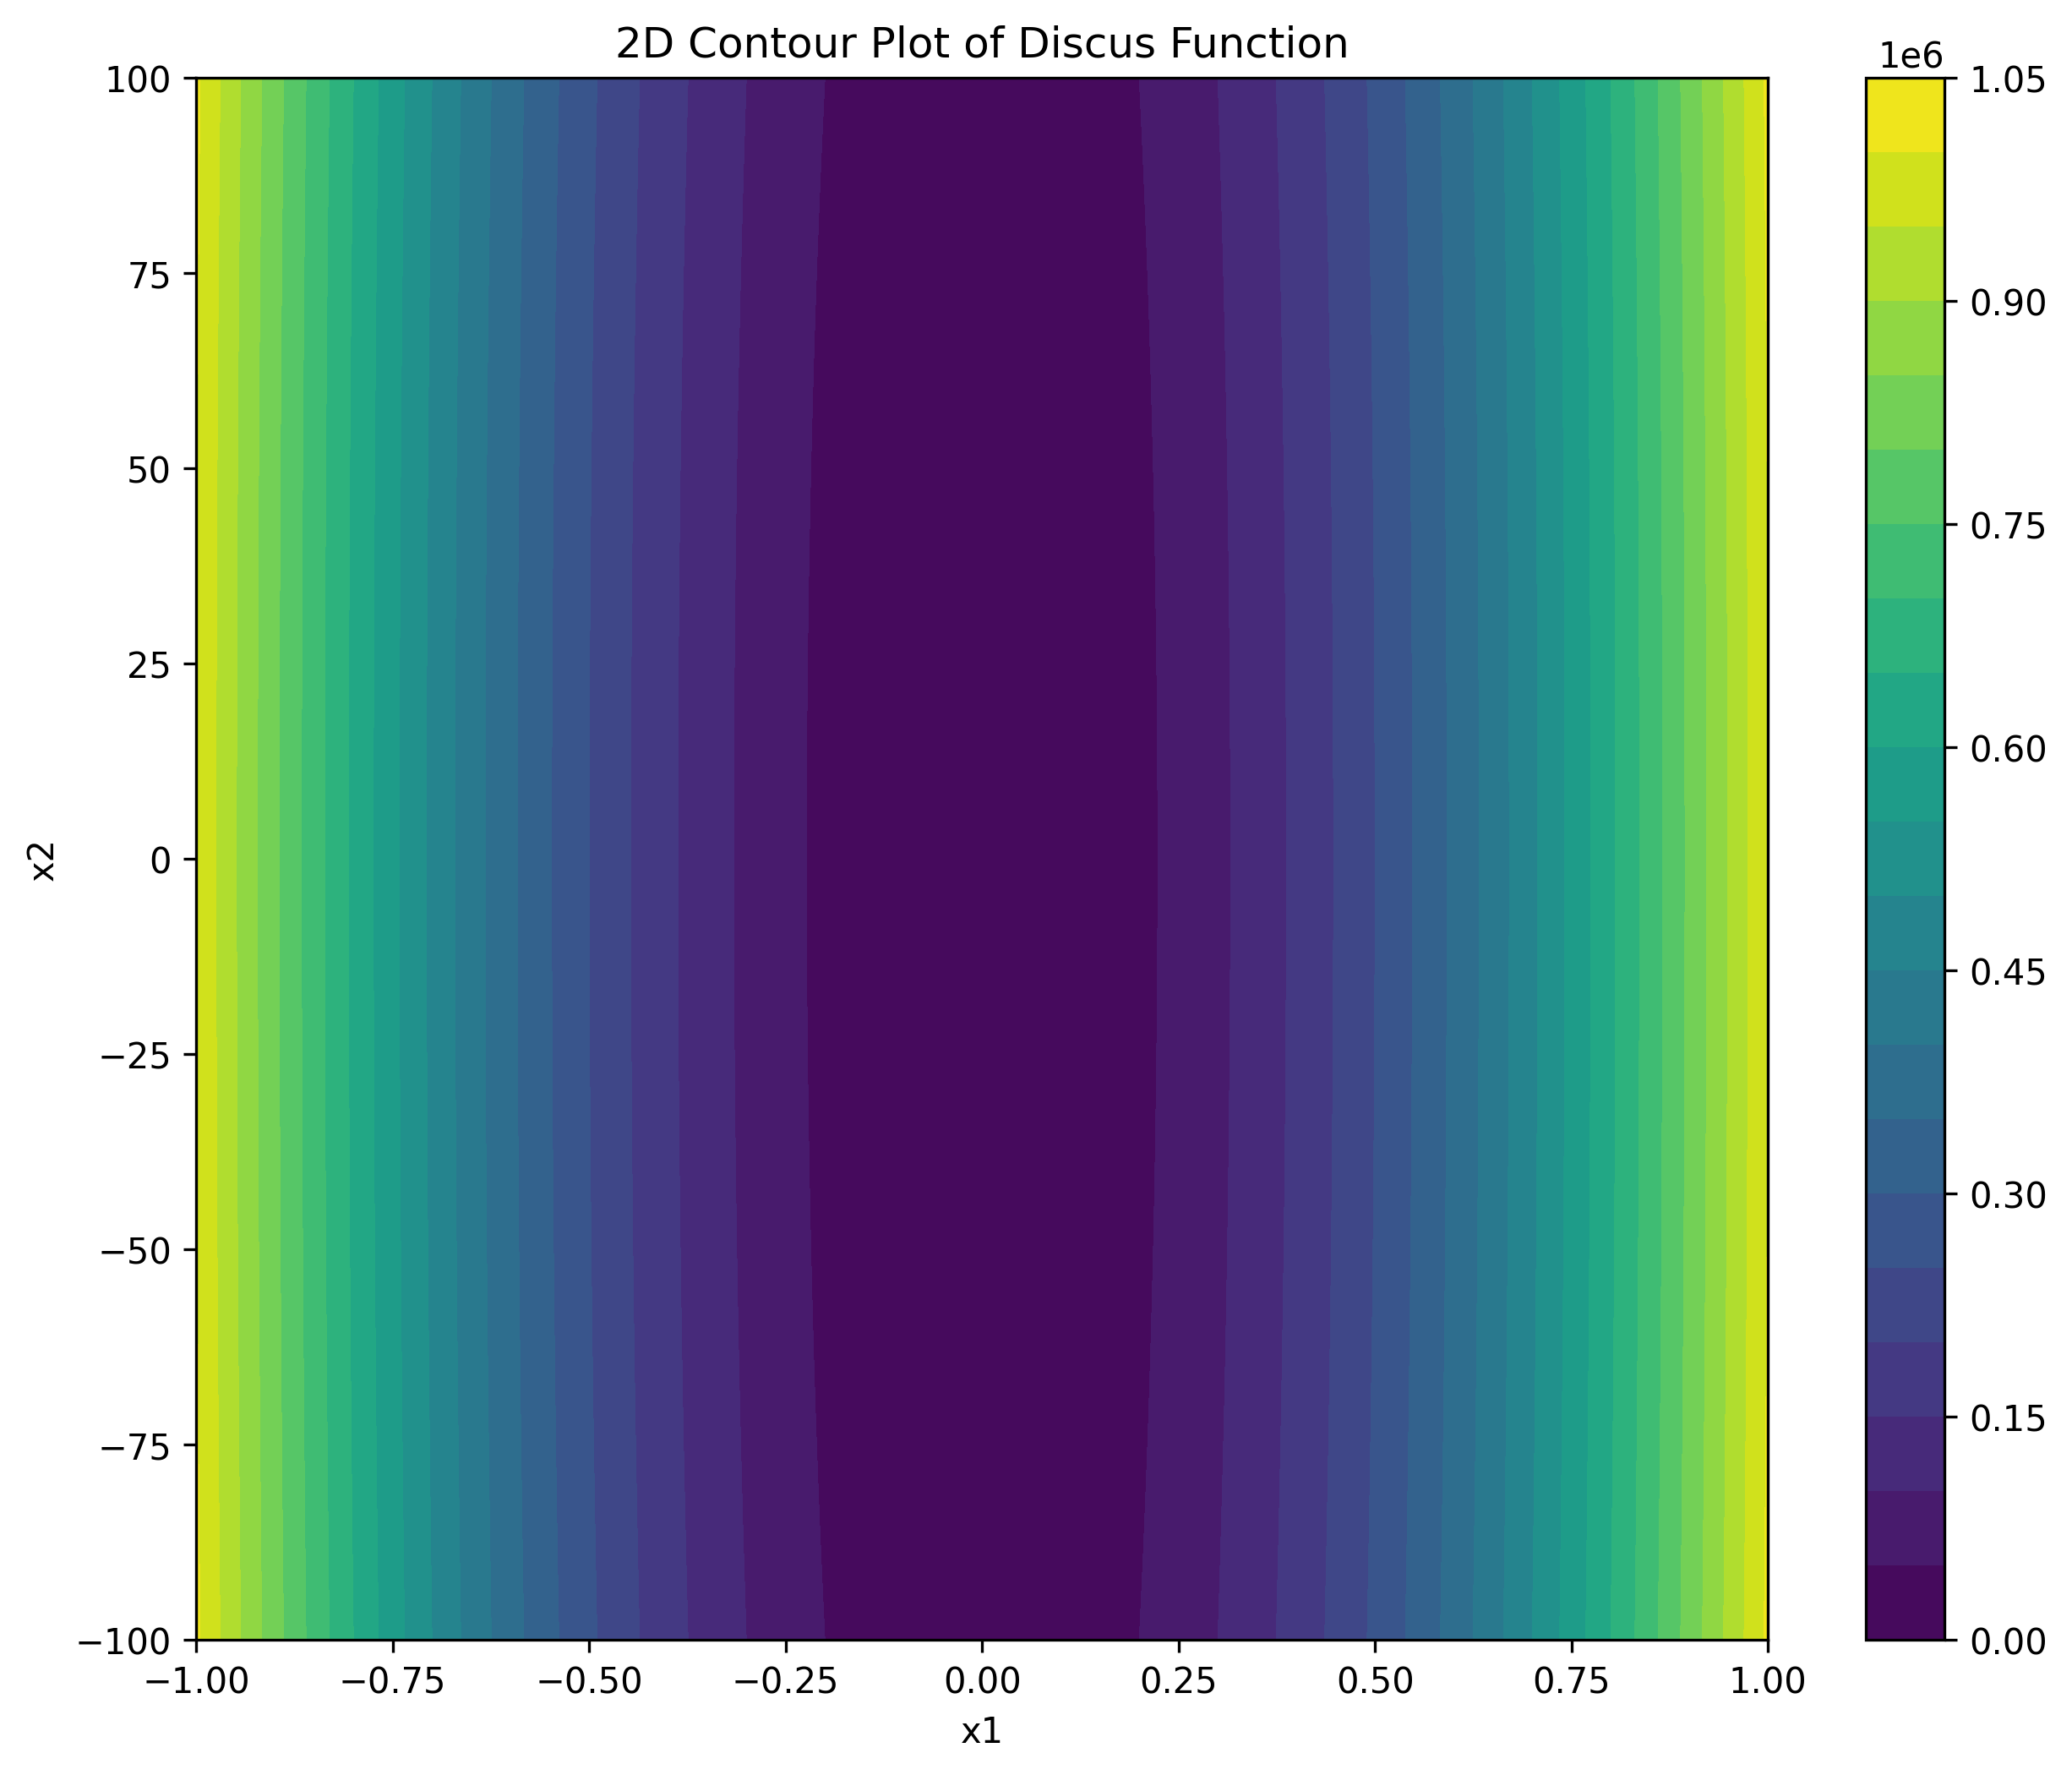
\includegraphics[width=\linewidth]{cec/discus_2d.png}
		\caption{Dimensi 2}
		\label{fig:discus-2d}
	\end{subfigure}
	\hfill
	\begin{subfigure}[b]{0.4\textwidth}
		\centering
		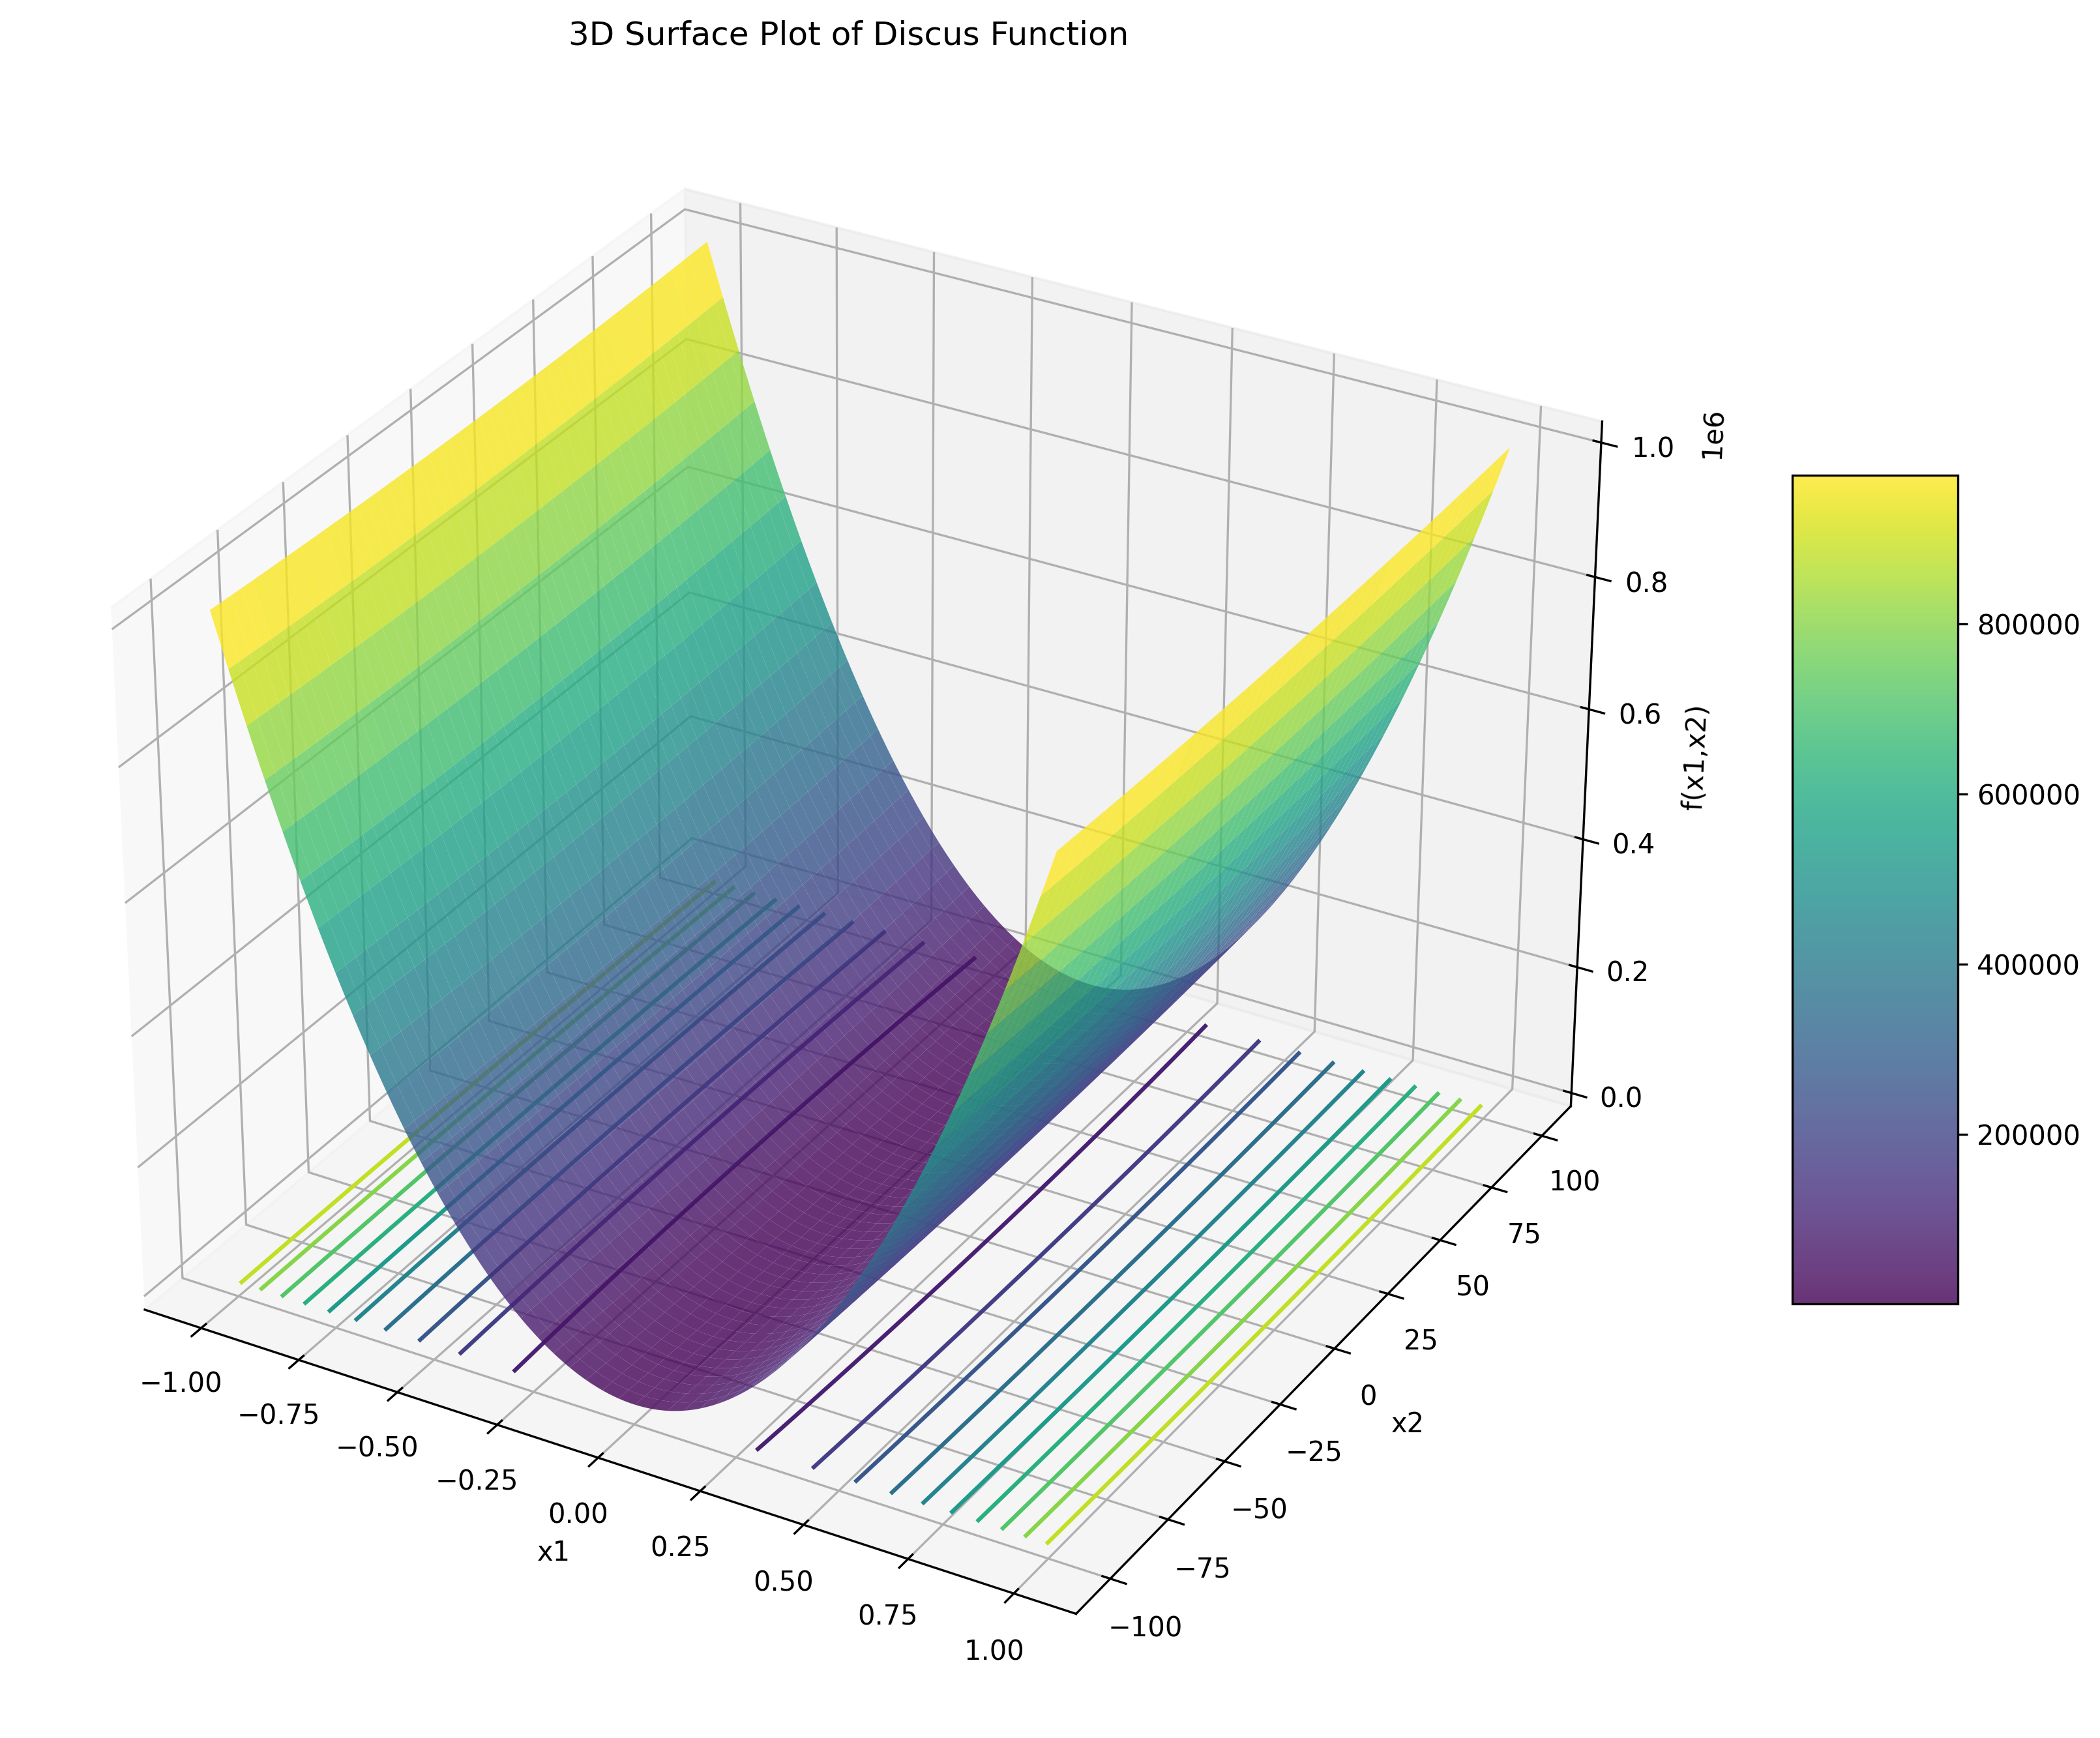
\includegraphics[width=\linewidth]{cec/discus_3d.png}
		\caption{Dimensi 3}
		\label{fig:discus-3d}
	\end{subfigure}
	\caption{Tampilan grafik fungsi Discus pada dimensi dua (\cref{fig:discus-2d}) dan tiga (\cref{fig:discus-3d})}
	\label{fig:discus}
\end{figure}
\begin{flalign*}
  f_{\text{Discus}}(\mathrm{x})=10^6z_1^2+\sum_{i=2}^{D}z_i^2+f_{\text{bias}}&&
\end{flalign*}

\subsubsection{Ellipsoid}
\noindent Properti:
\begin{packed_item}
  \item unimodal
  \item convex
\end{packed_item}
\begin{figure}[H]
	\centering
	\begin{subfigure}[b]{0.4\textwidth}
		\centering
		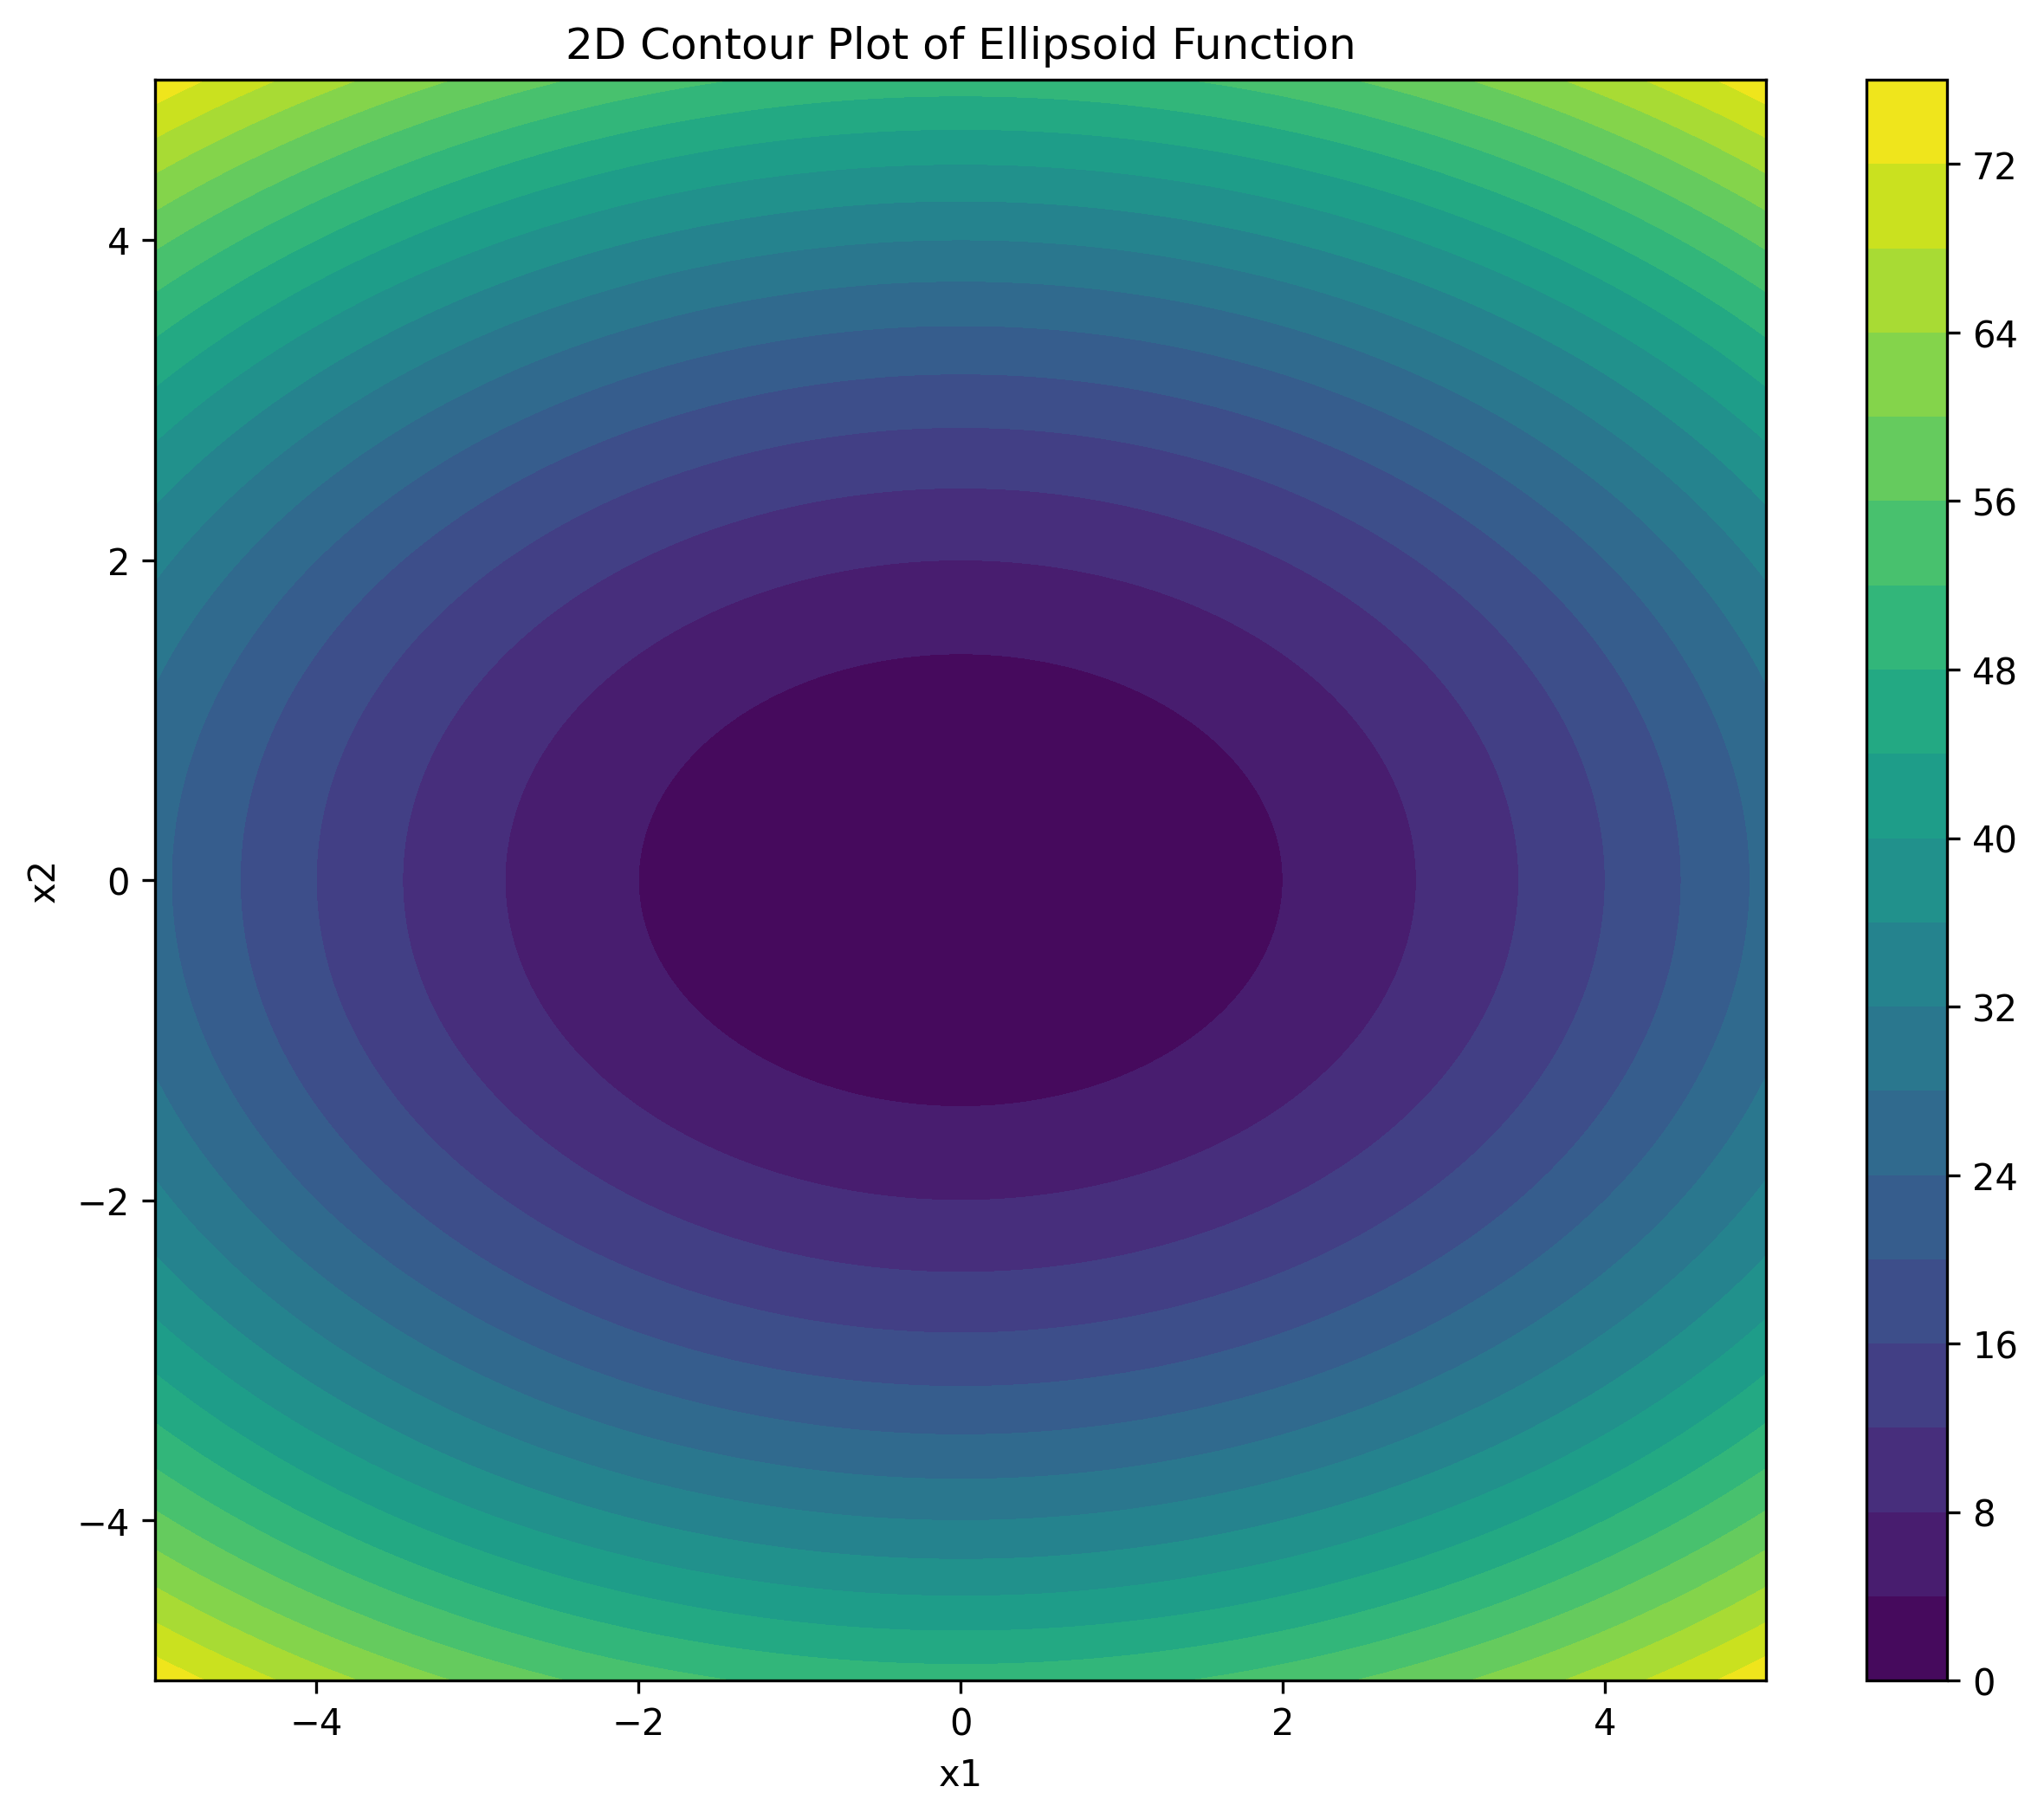
\includegraphics[width=\linewidth]{cec/ellipsoid_2d.png}
		\caption{Dimensi 2}
		\label{fig:ellipsoid-2d}
	\end{subfigure}
	\hfill
	\begin{subfigure}[b]{0.4\textwidth}
		\centering
		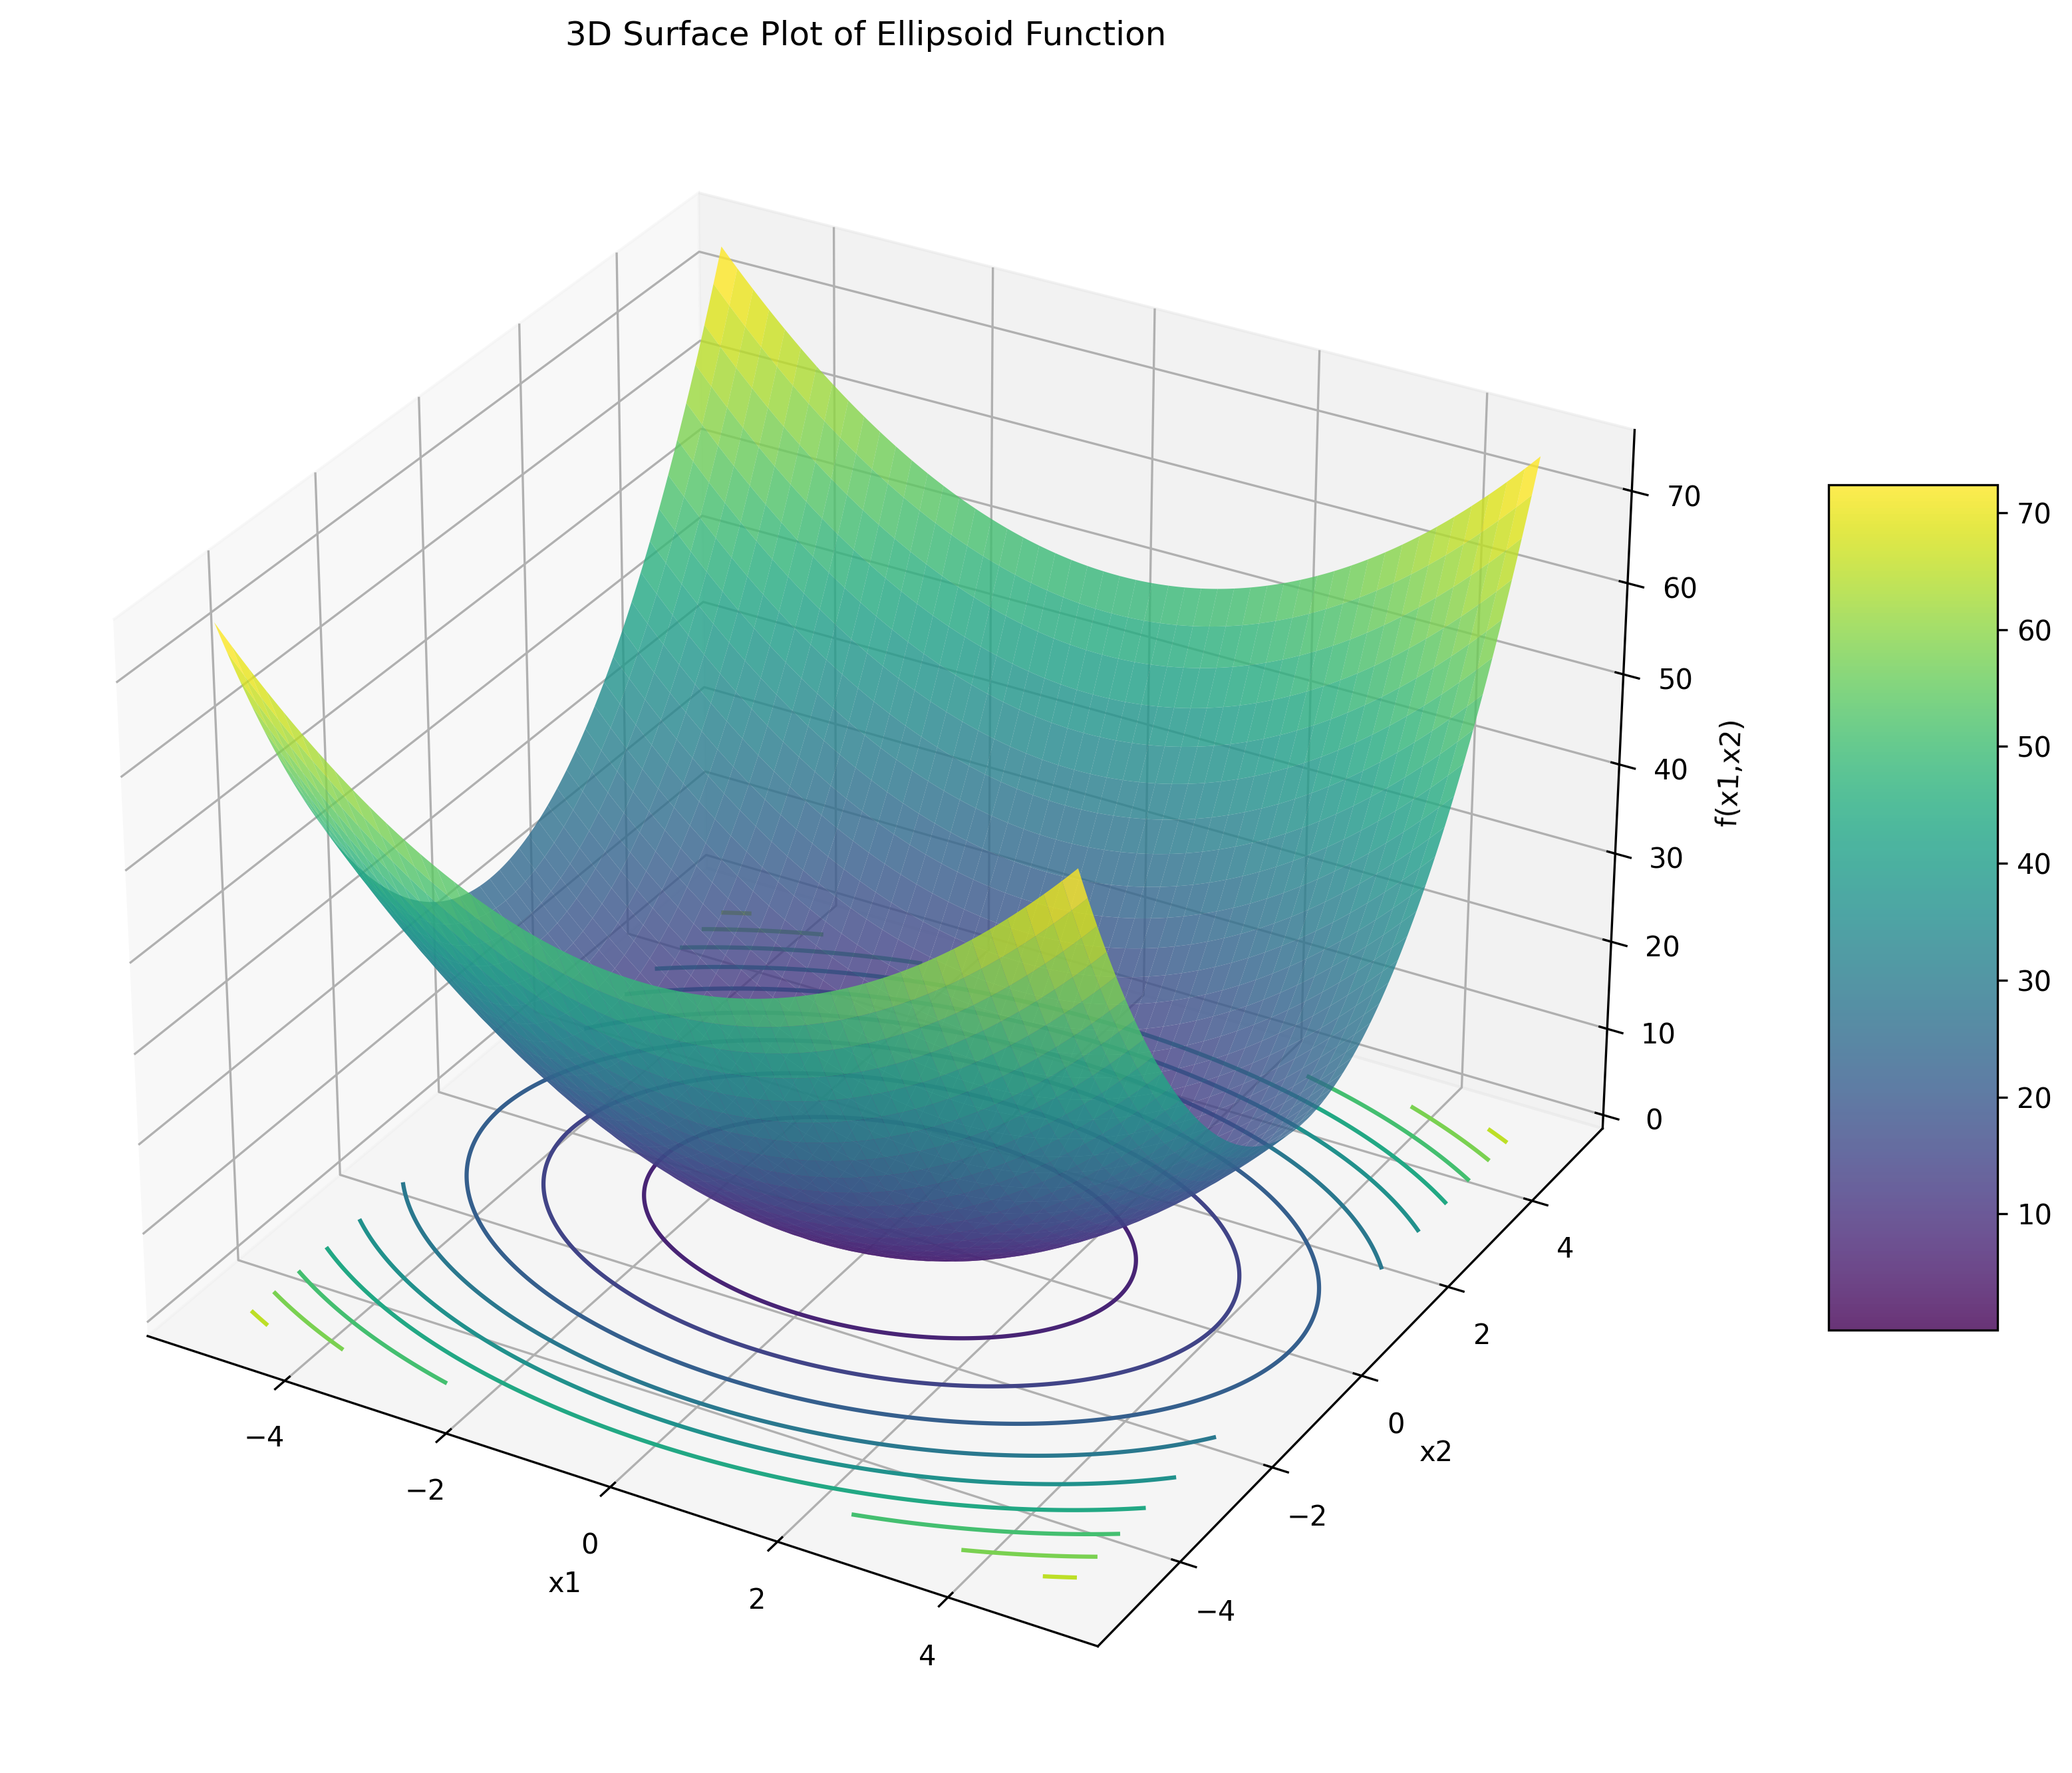
\includegraphics[width=\linewidth]{cec/ellipsoid_3d.png}
		\caption{Dimensi 3}
		\label{fig:ellipsoid-3d}
	\end{subfigure}
	\caption{Tampilan grafik fungsi Ellipsoid pada dimensi dua (\cref{fig:ellipsoid-2d}) dan tiga (\cref{fig:ellipsoid-3d})}
	\label{fig:ellipsoid}
\end{figure}
\begin{flalign*}
  f_{\text{Ellipsoid}}(\mathrm{x})=\sum_{i=1}^{D}iz_i^2  +f_{\text{bias}}&&
\end{flalign*}

\subsubsection{Elliptic}
\noindent Properti:
\begin{packed_item}
  \item unimodal
  \item convex
  \item non-separable
  \item quadric ill-conditioned
  \item smooth local irregularities
\end{packed_item}
\begin{figure}[H]
	\centering
	\begin{subfigure}[b]{0.4\textwidth}
		\centering
		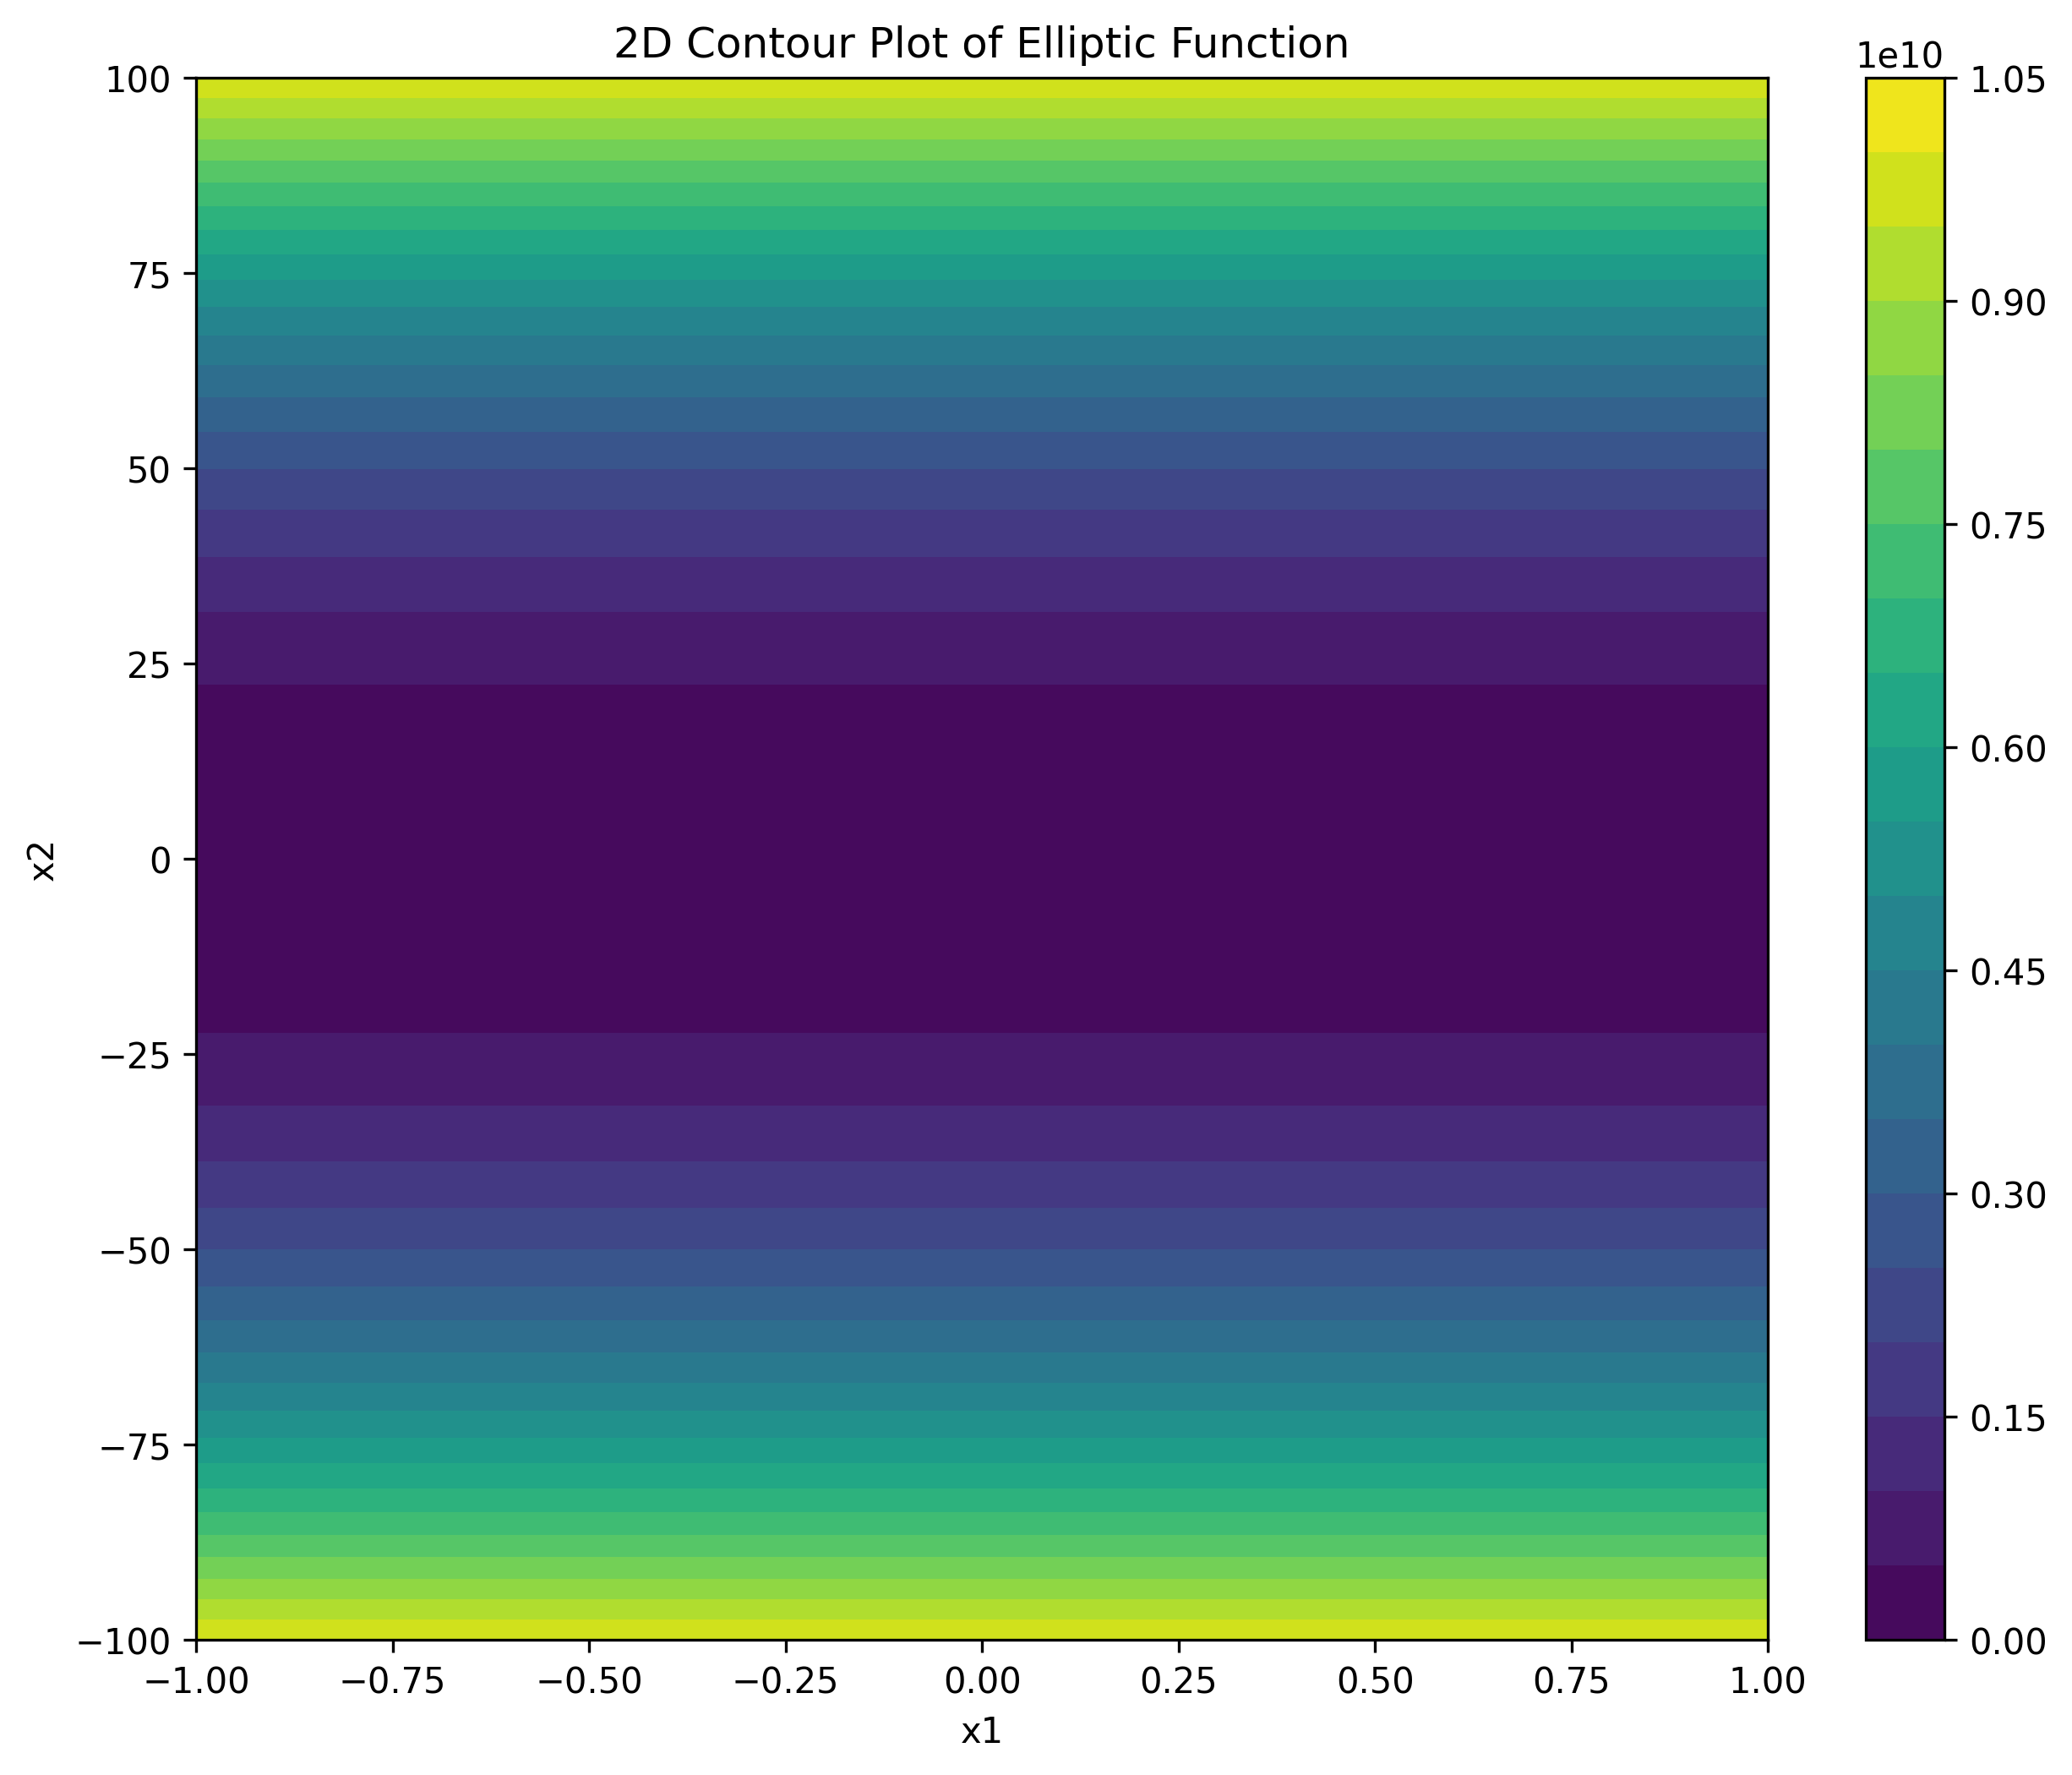
\includegraphics[width=\linewidth]{cec/elliptic_2d.png}
		\caption{Dimensi 2}
		\label{fig:elliptic-2d}
	\end{subfigure}
	\hfill
	\begin{subfigure}[b]{0.4\textwidth}
		\centering
		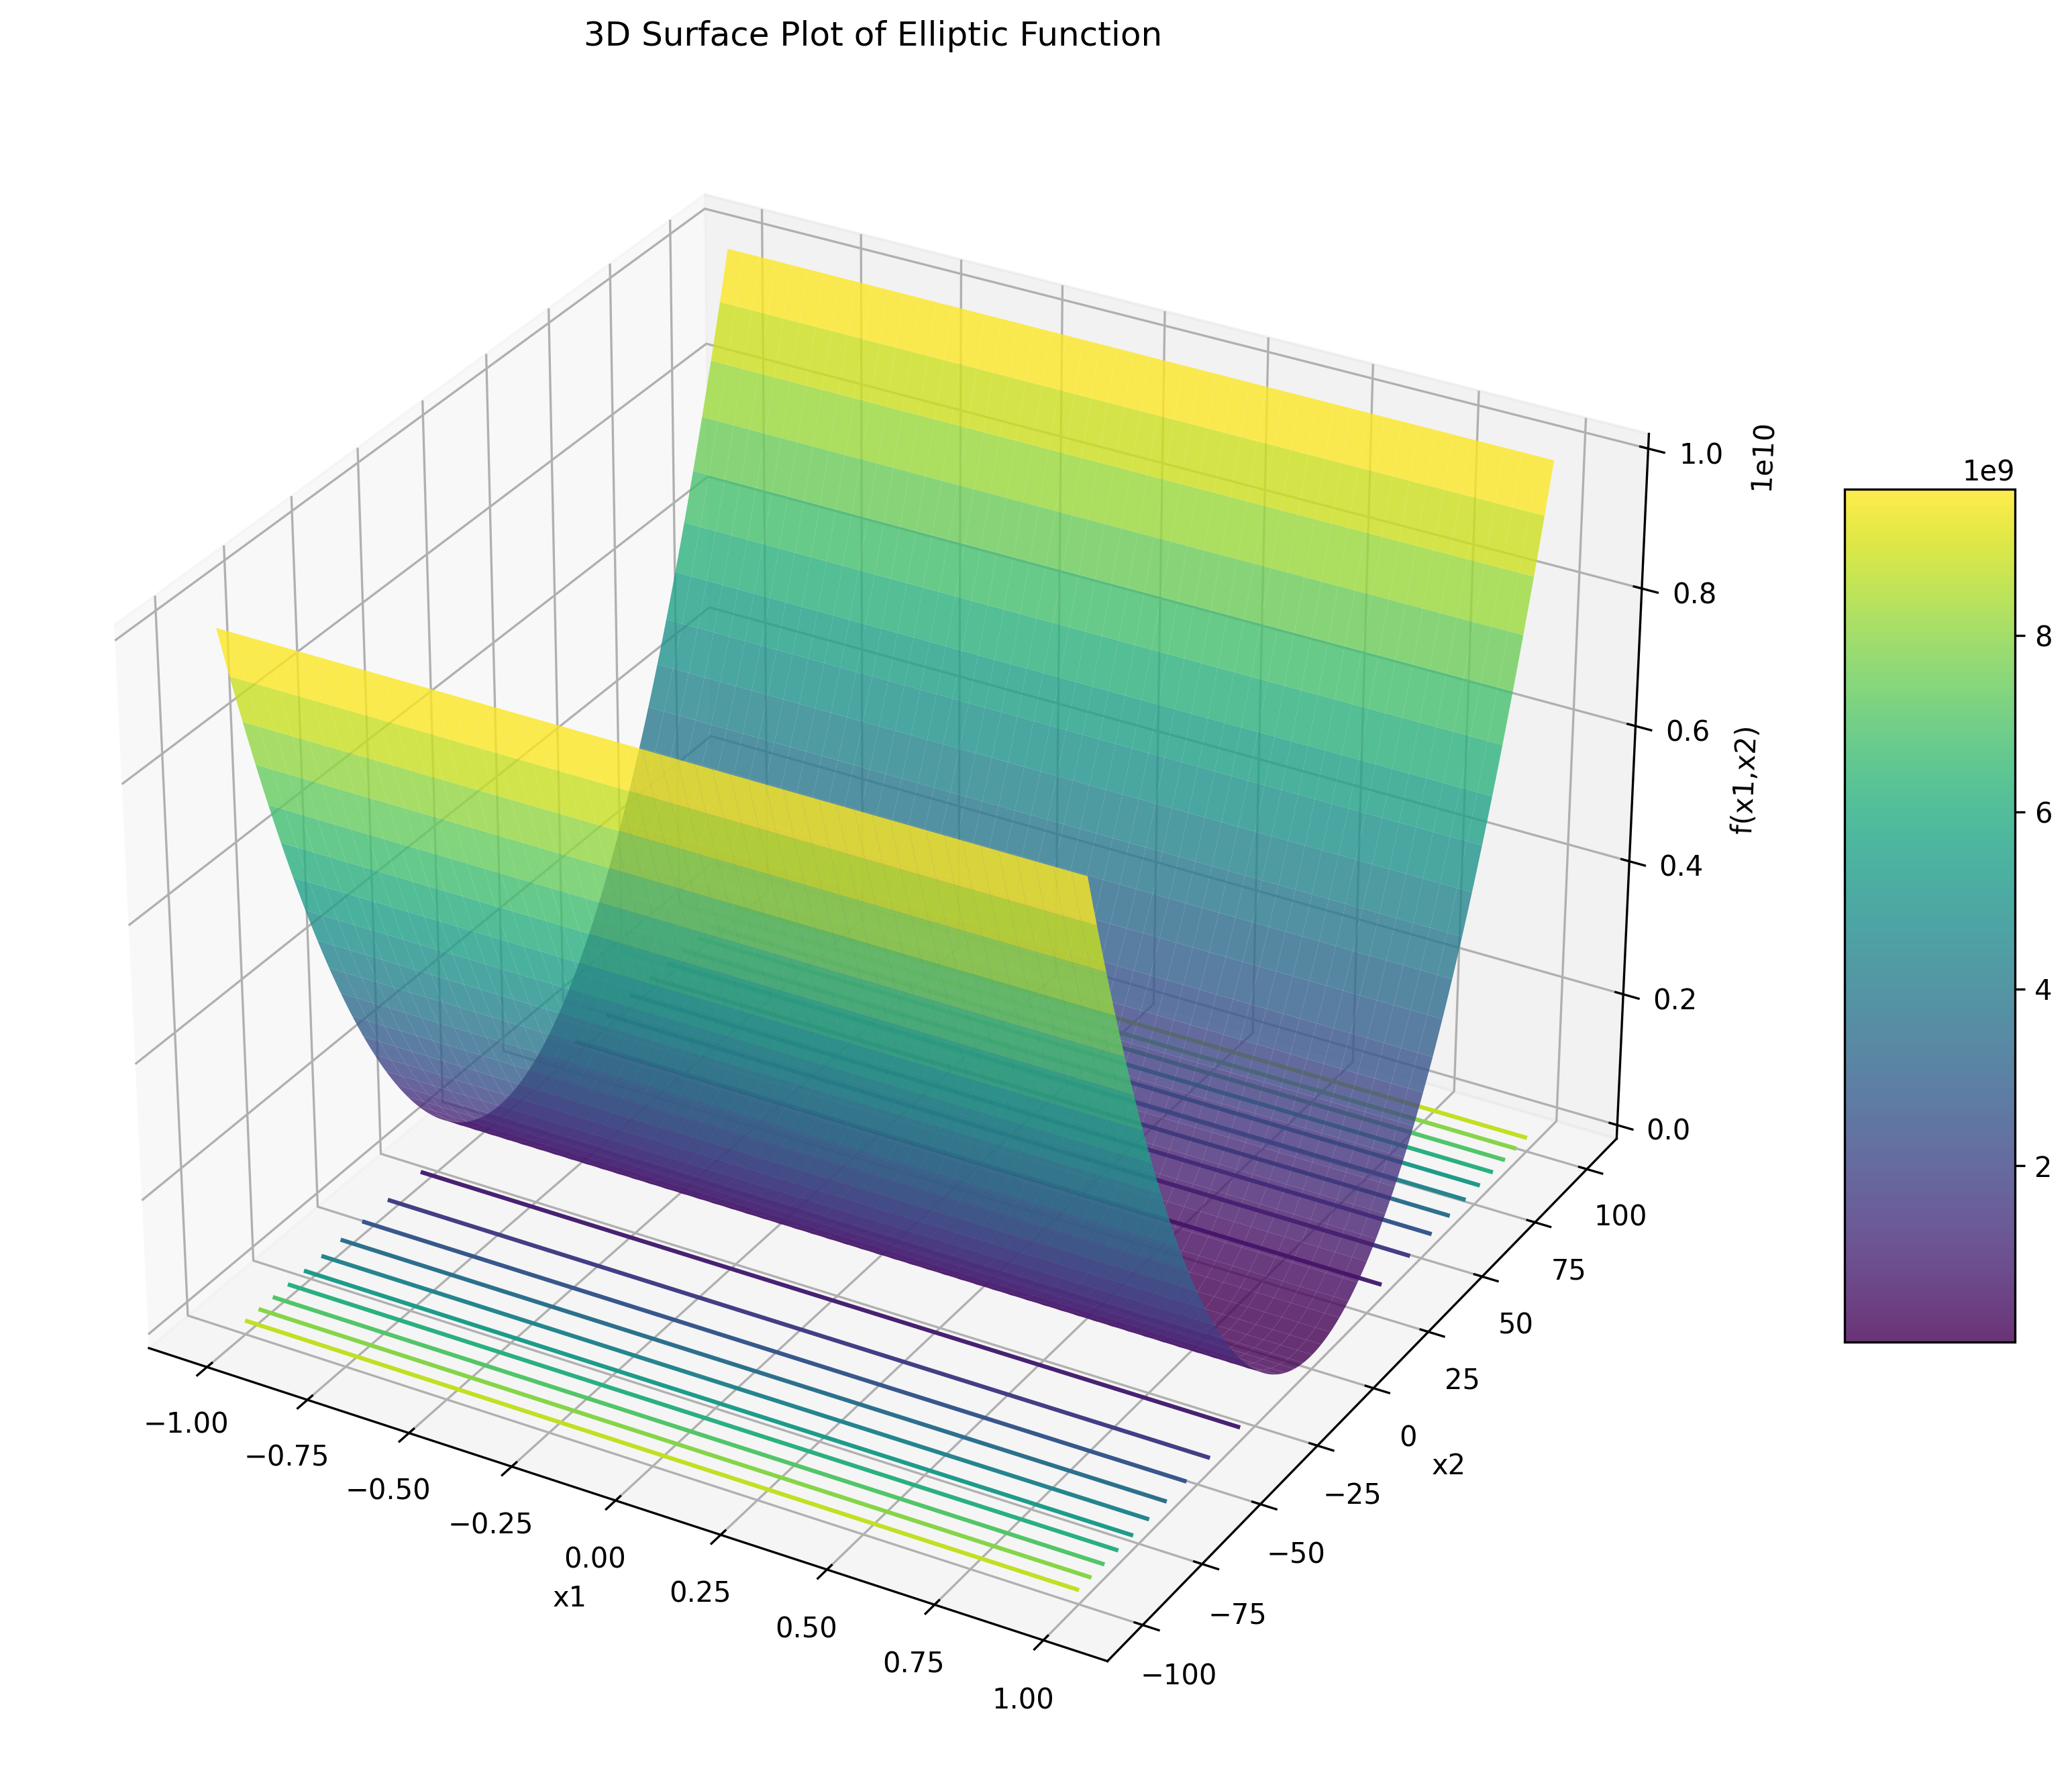
\includegraphics[width=\linewidth]{cec/elliptic_3d.png}
		\caption{Dimensi 3}
		\label{fig:elliptic-3d}
	\end{subfigure}
	\caption{Tampilan grafik fungsi Elliptic pada dimensi dua (\cref{fig:elliptic-2d}) dan tiga (\cref{fig:elliptic-3d})}
	\label{fig:elliptic}
\end{figure}
\begin{flalign*}
  f_{\text{Elliptic}}(\mathrm{x})= \sum_{i=1}^{D} \left( 10^6\right)^{\frac{i-1}{D-1}} z_i^2 +f_{\text{bias}}&&
\end{flalign*}

\subsubsection{Expanded schaffer f6}
\noindent Properti:
\begin{packed_item}
  \item multimodal
  \item non-convex
  \item non-separable
\end{packed_item}
\begin{figure}[H]
	\centering
	\begin{subfigure}[b]{0.4\textwidth}
		\centering
		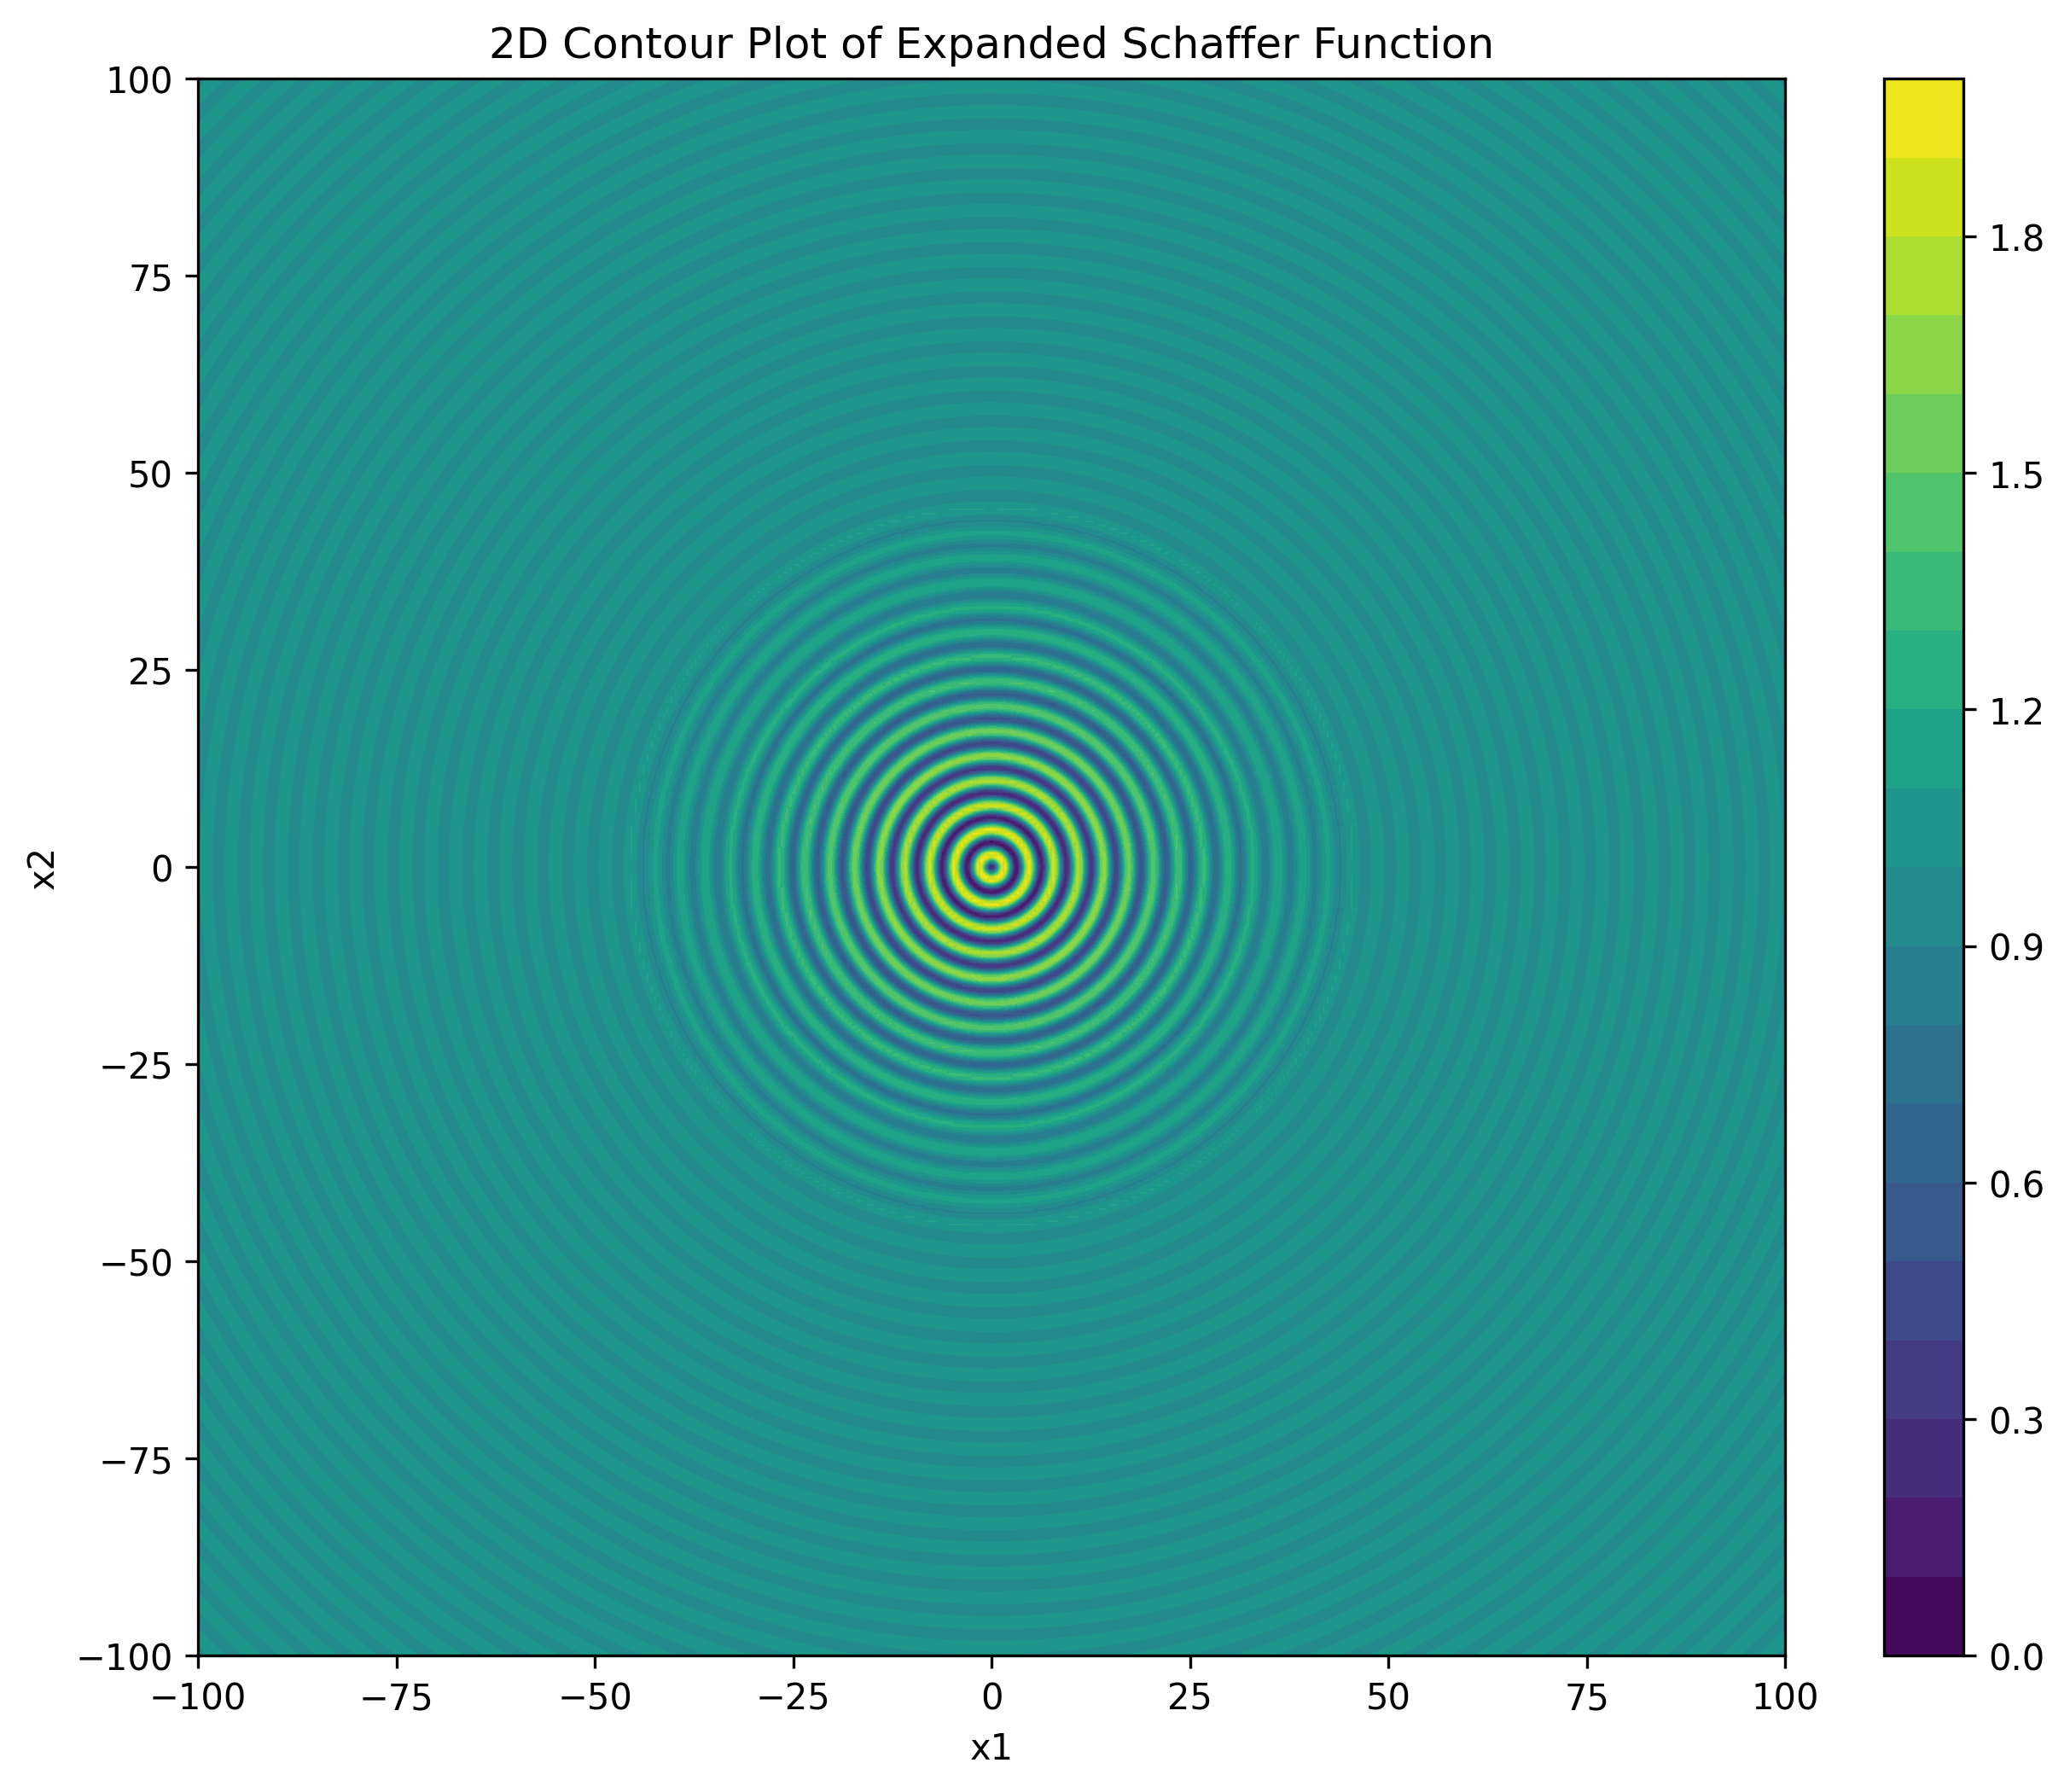
\includegraphics[width=\linewidth]{cec/expanded_schaffer_2d.png}
		\caption{Dimensi 2}
		\label{fig:schaffer-2d}
	\end{subfigure}
	\hfill
	\begin{subfigure}[b]{0.4\textwidth}
		\centering
		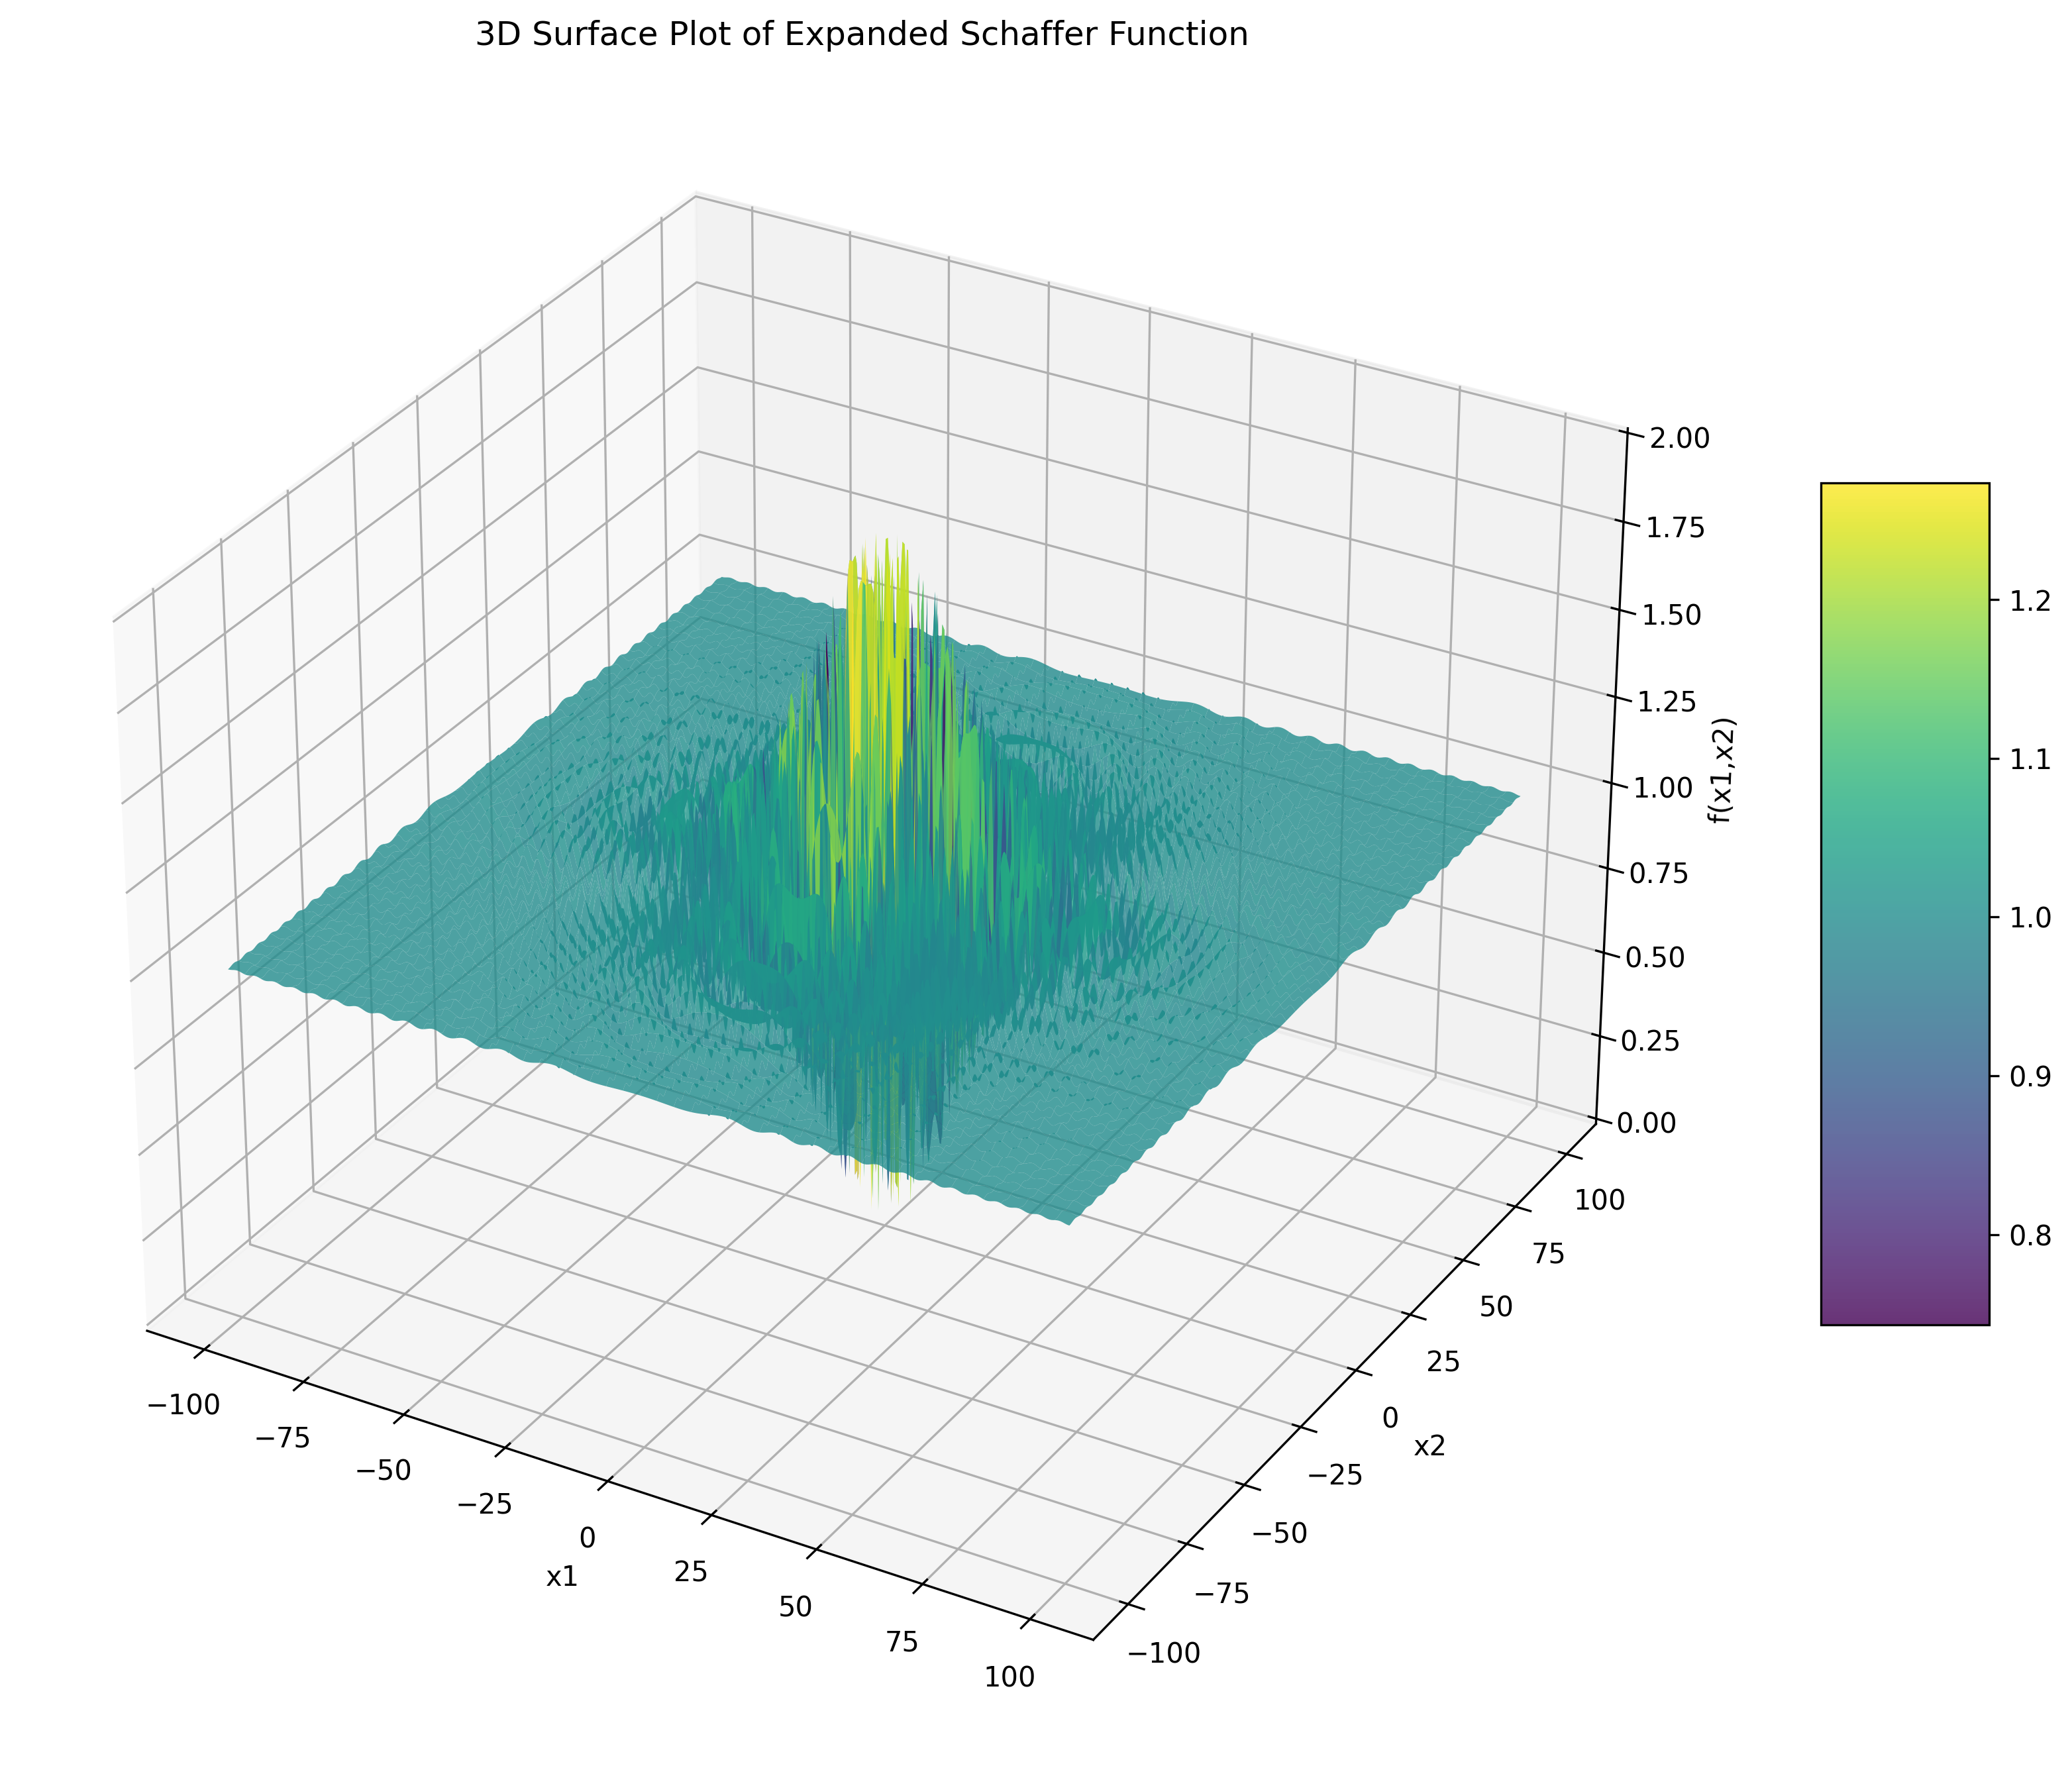
\includegraphics[width=\linewidth]{cec/expanded_schaffer_3d.png}
		\caption{Dimensi 3}
		\label{fig:schaffer-3d}
	\end{subfigure}
	\caption{Tampilan grafik fungsi Expanded schaffer f6 pada dimensi dua (\cref{fig:schaffer-2d}) dan tiga (\cref{fig:schaffer-3d})}
	\label{fig:schaffer}
\end{figure}
\begin{flalign*}
  &g\left(x,y \right)=0.5+\frac{\sin^2\left(\sqrt{x^2+y^2} \right)-0.5 }{\left( 1+0.0001\left(x^2+y^2 \right) \right)^2 }&&\\
  &f_{\text{Expanded schaffer f6}}(\mathrm{x})=g\left(z_1,z_2 \right)+g\left(z_2,z_3 \right)+\ldots+g\left(z_{D-1},z_D \right)+g\left(z_D,z_1 \right)+f_{\text{bias}}&&
\end{flalign*}

\subsubsection{Griewank}
\noindent Properti:
\begin{packed_item}
  \item multimodal
  \item non-convex
  \item non-separable
  \item scalable
\end{packed_item}
\begin{figure}[H]
	\centering
	\begin{subfigure}[b]{0.4\textwidth}
		\centering
		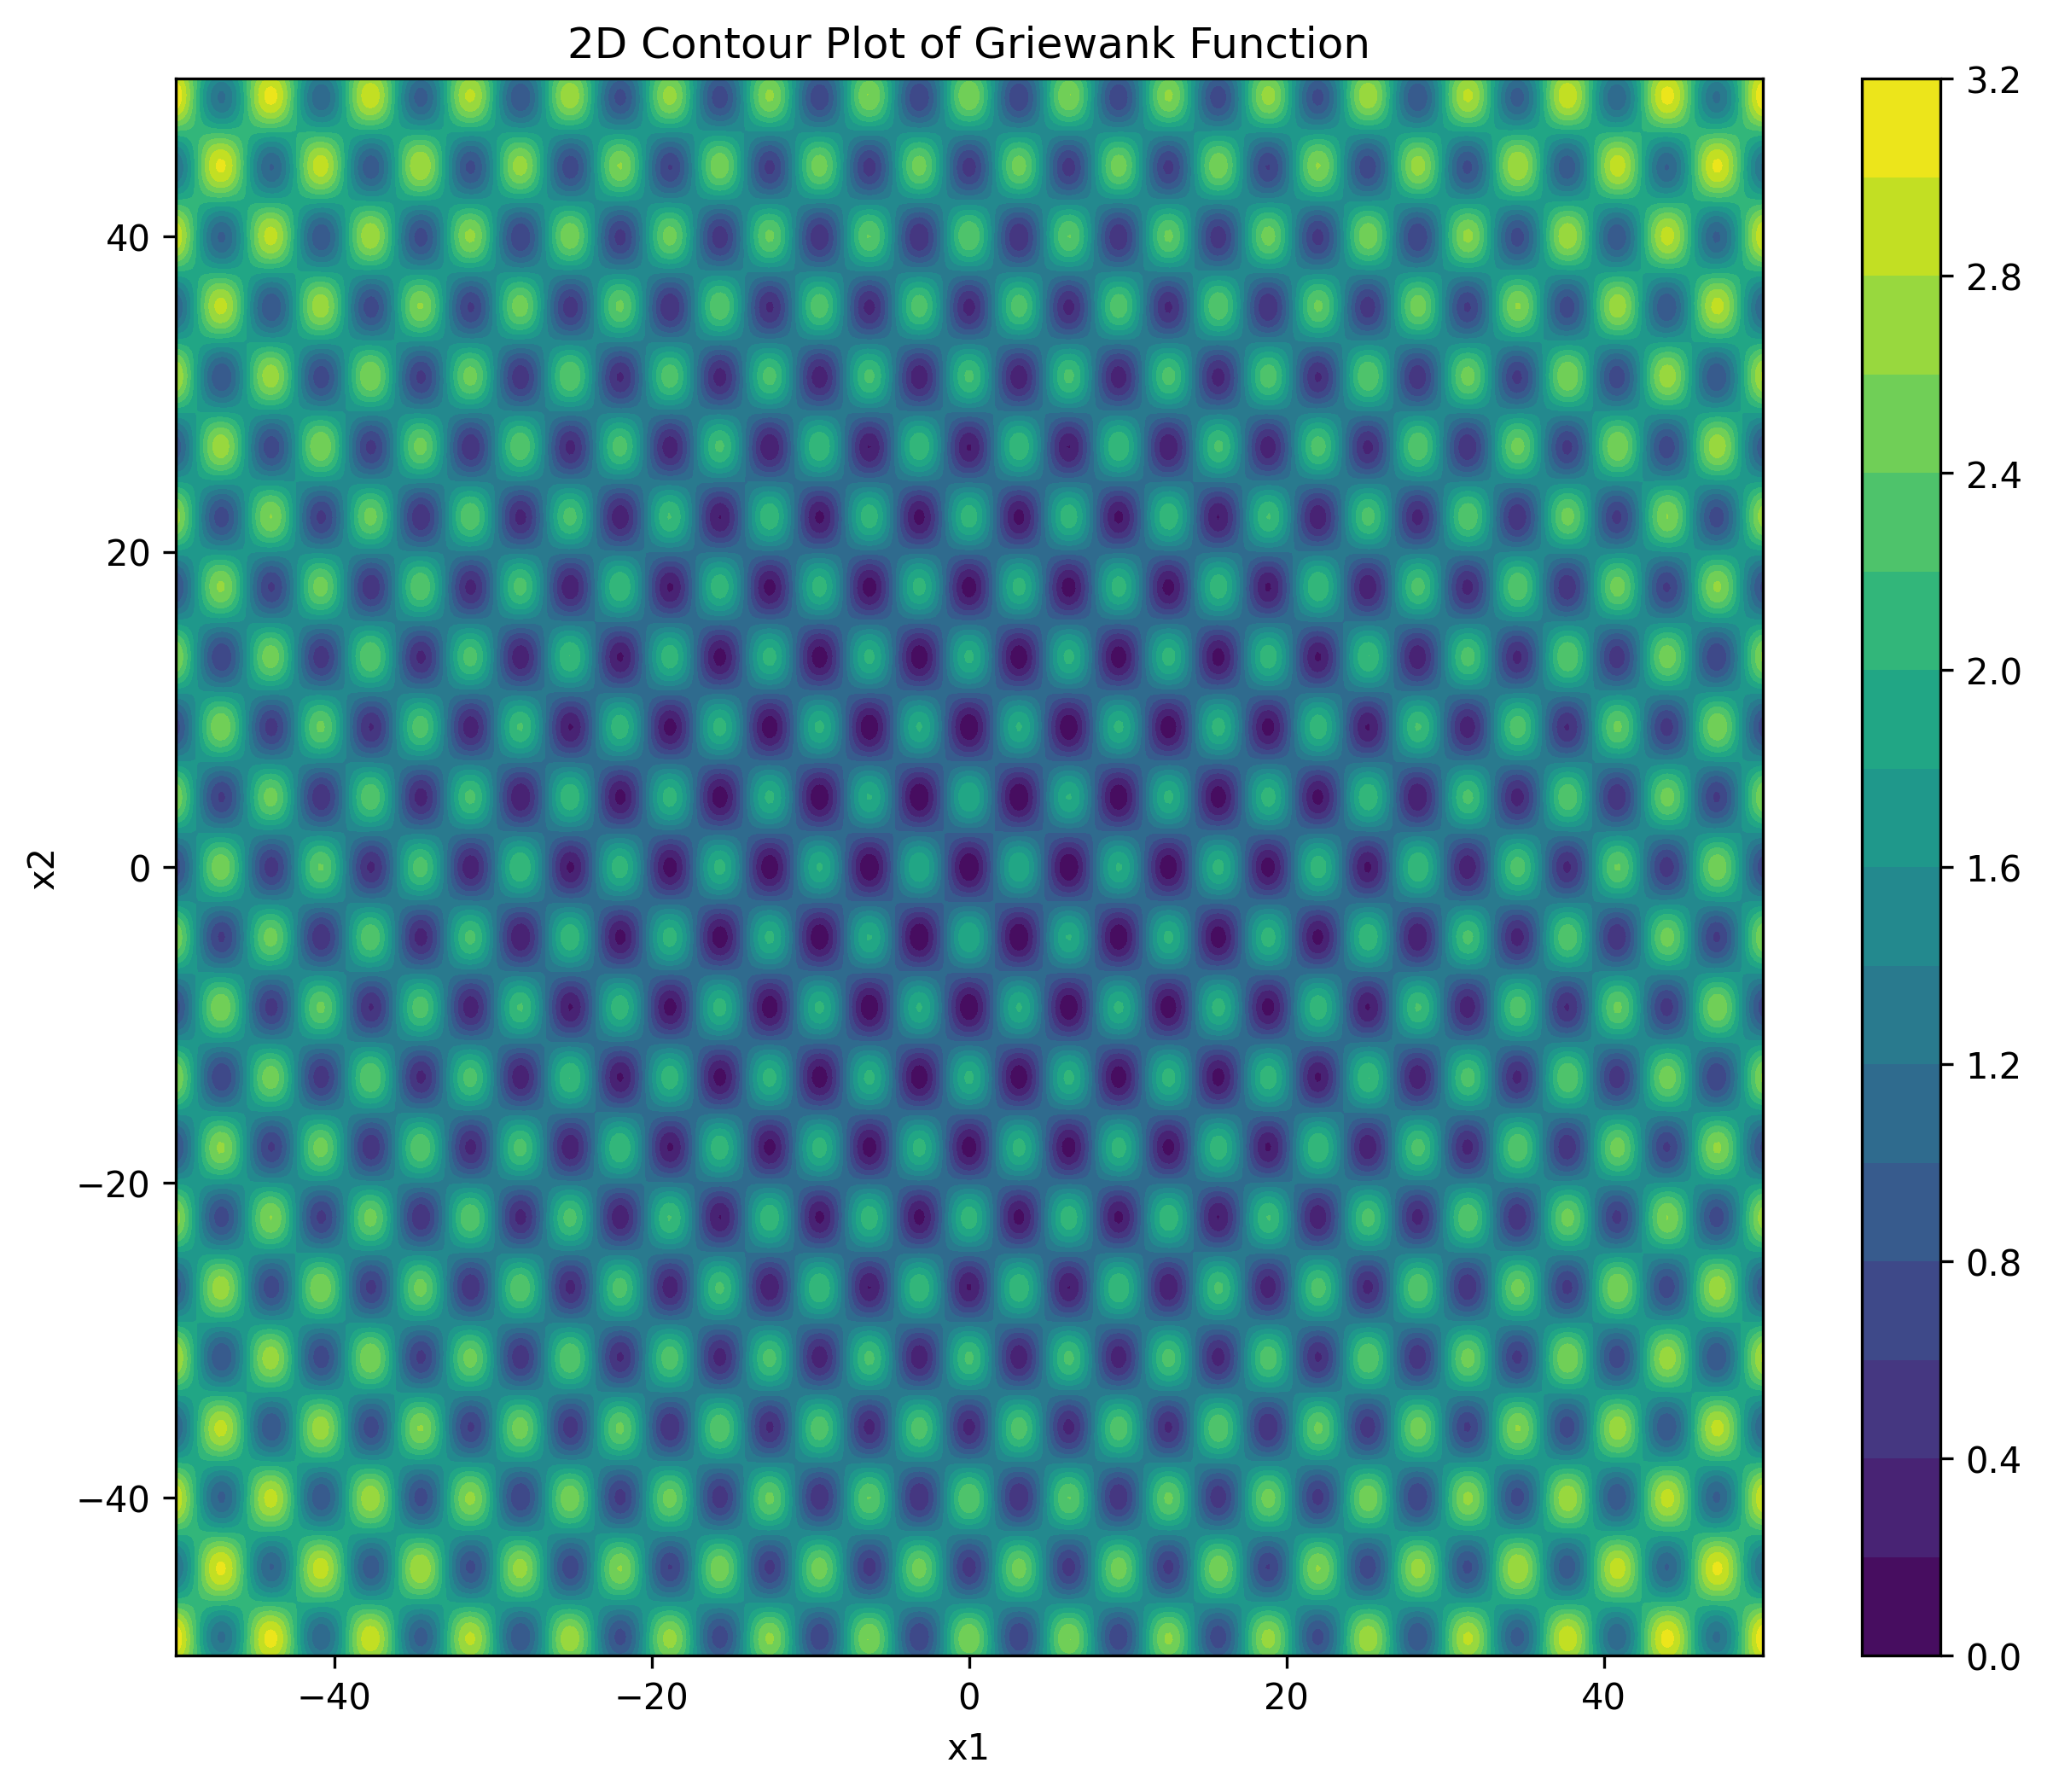
\includegraphics[width=\linewidth]{cec/griewank_2d.png}
		\caption{Dimensi 2}
		\label{fig:griewank-2d}
	\end{subfigure}
	\hfill
	\begin{subfigure}[b]{0.4\textwidth}
		\centering
		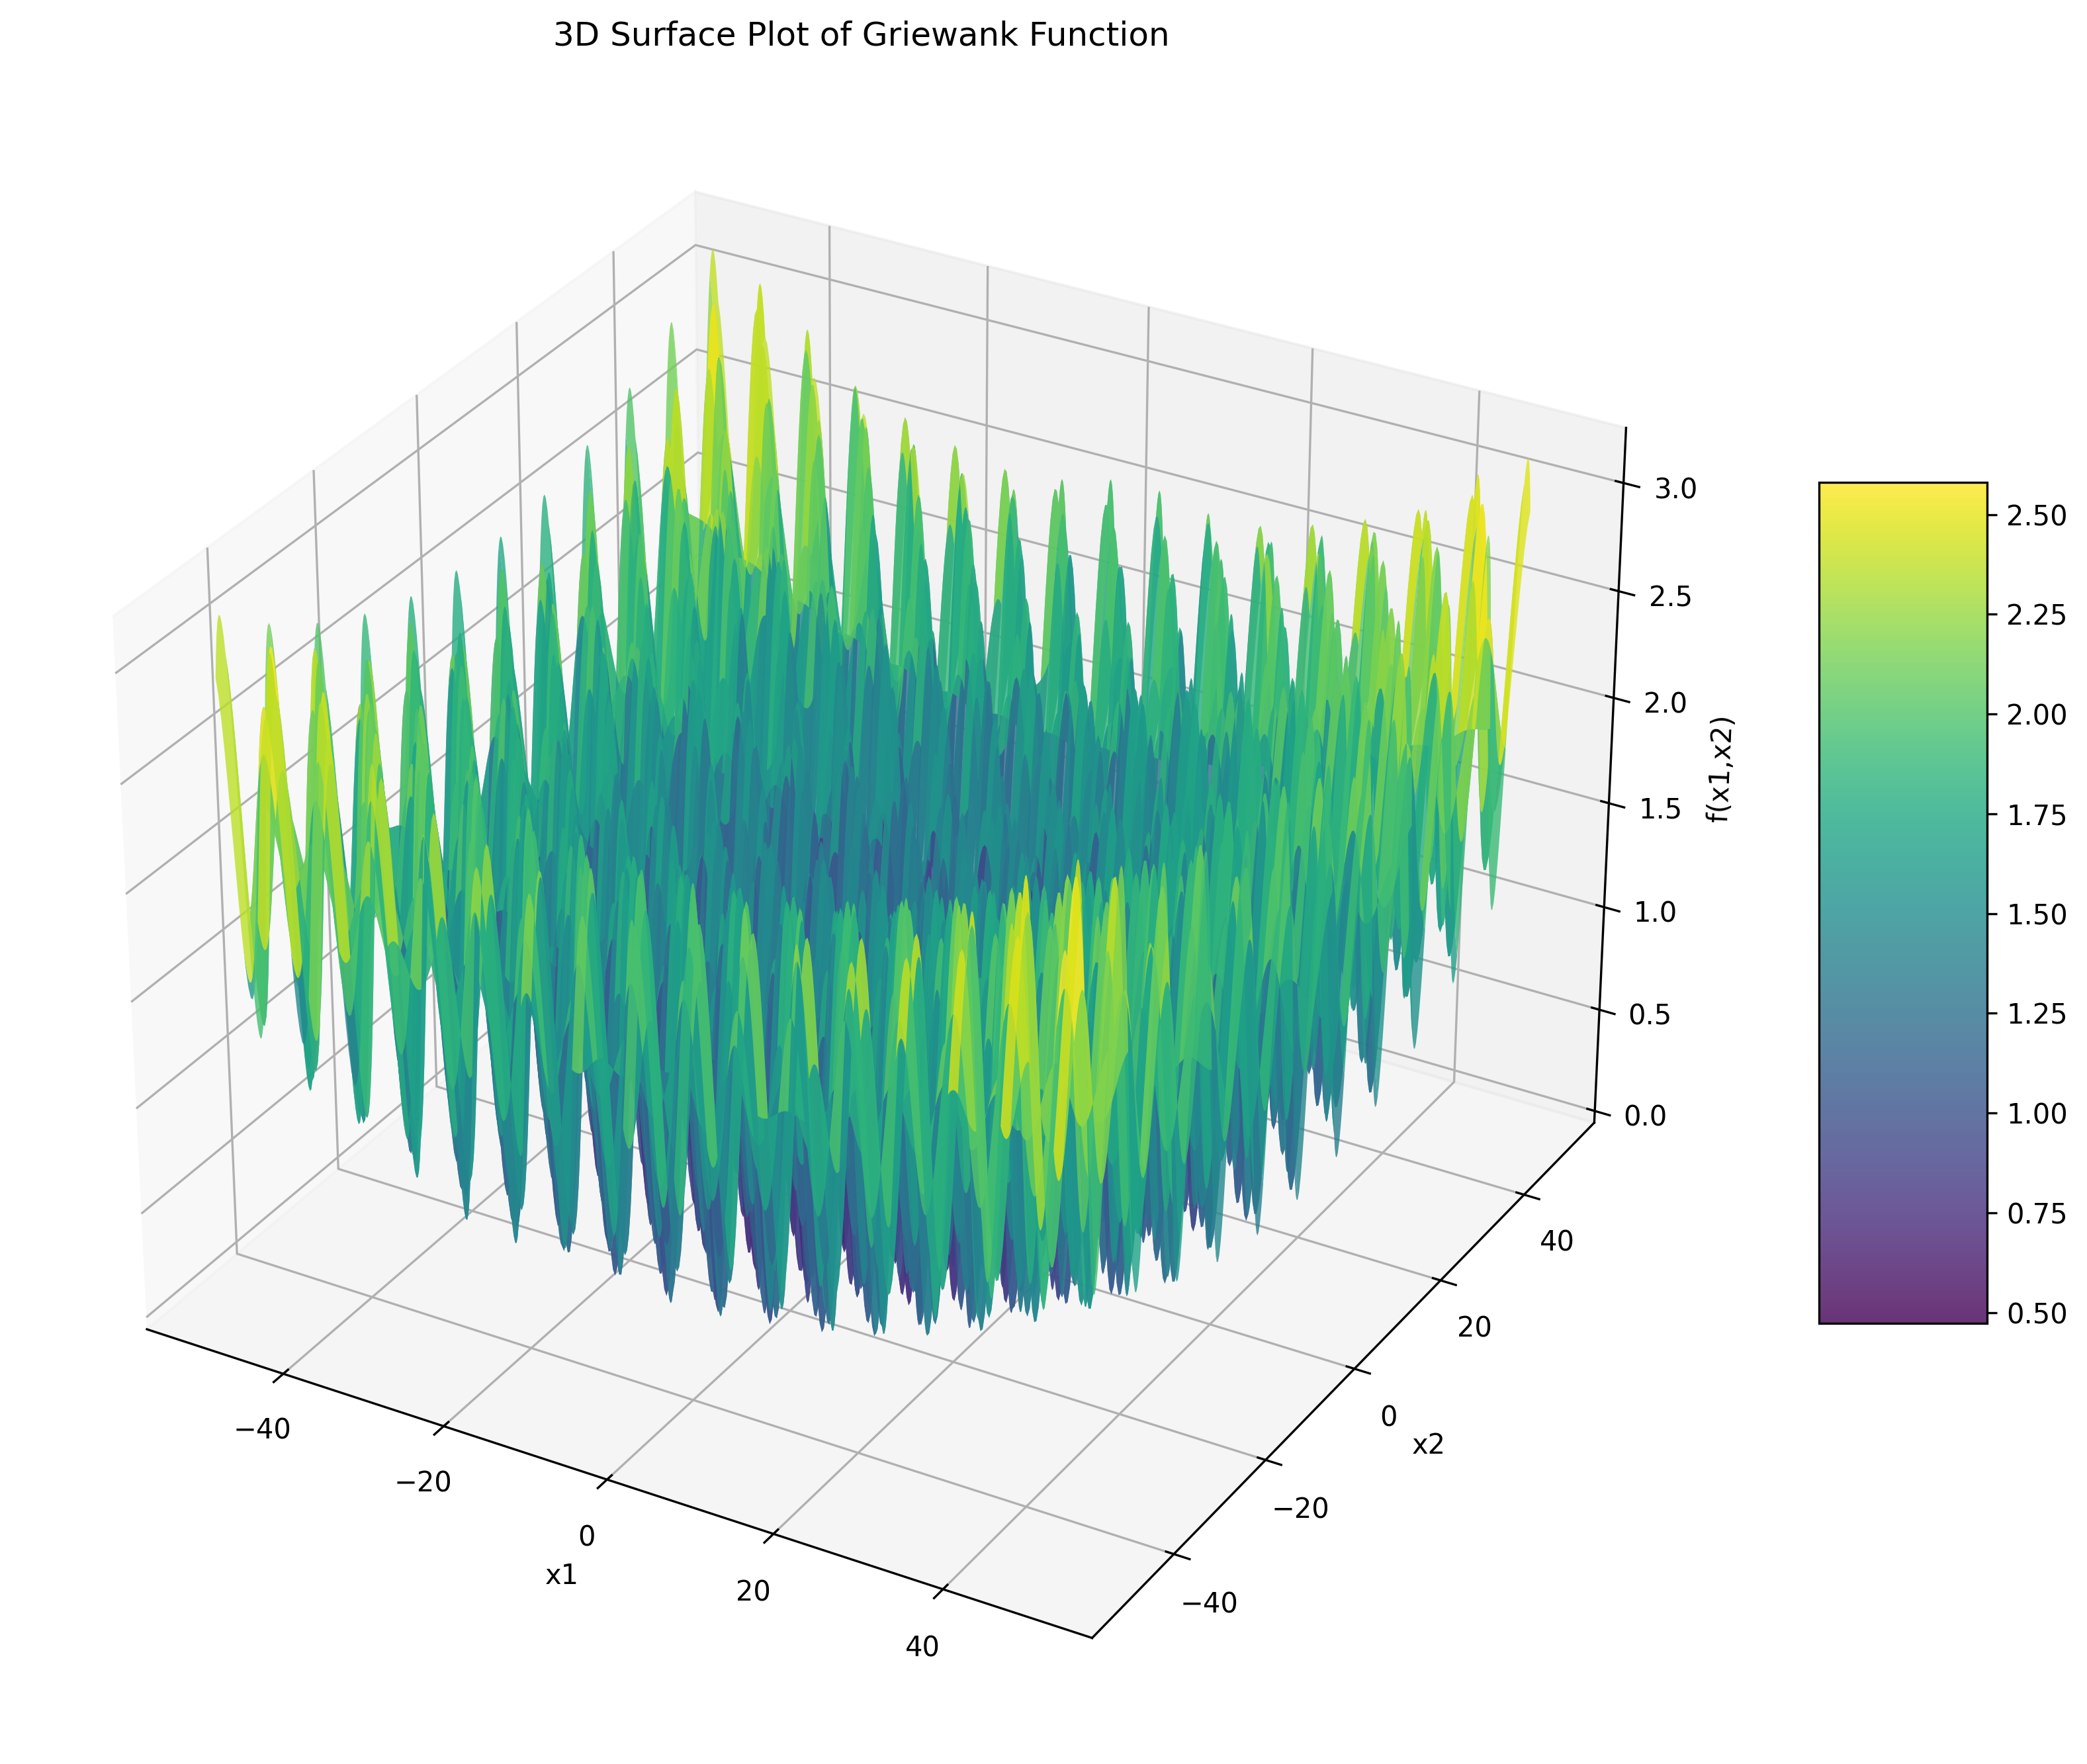
\includegraphics[width=\linewidth]{cec/griewank_3d.png}
		\caption{Dimensi 3}
		\label{fig:griewank-3d}
	\end{subfigure}
	\caption{Tampilan grafik fungsi Griewank pada dimensi dua (\cref{fig:griewank-2d}) dan tiga (\cref{fig:griewank-3d})}
	\label{fig:griewank}
\end{figure}
\begin{flalign*}
  f_{\text{Griewank}}(\mathrm{x})=\sum_{i=1}^{D}\frac{z_i^2}{4000}-\prod_{i=1}^{D}\cos\left( \frac{z_i}{\sqrt{i}}\right)+1 +f_{\text{bias}}&&
\end{flalign*}

\subsubsection{Happycat}
\noindent Properti:
\begin{packed_item}
  \item multimodal
  \item non-convex
  \item non-separable
\end{packed_item}
\begin{figure}[H]
	\centering
	\begin{subfigure}[b]{0.4\textwidth}
		\centering
		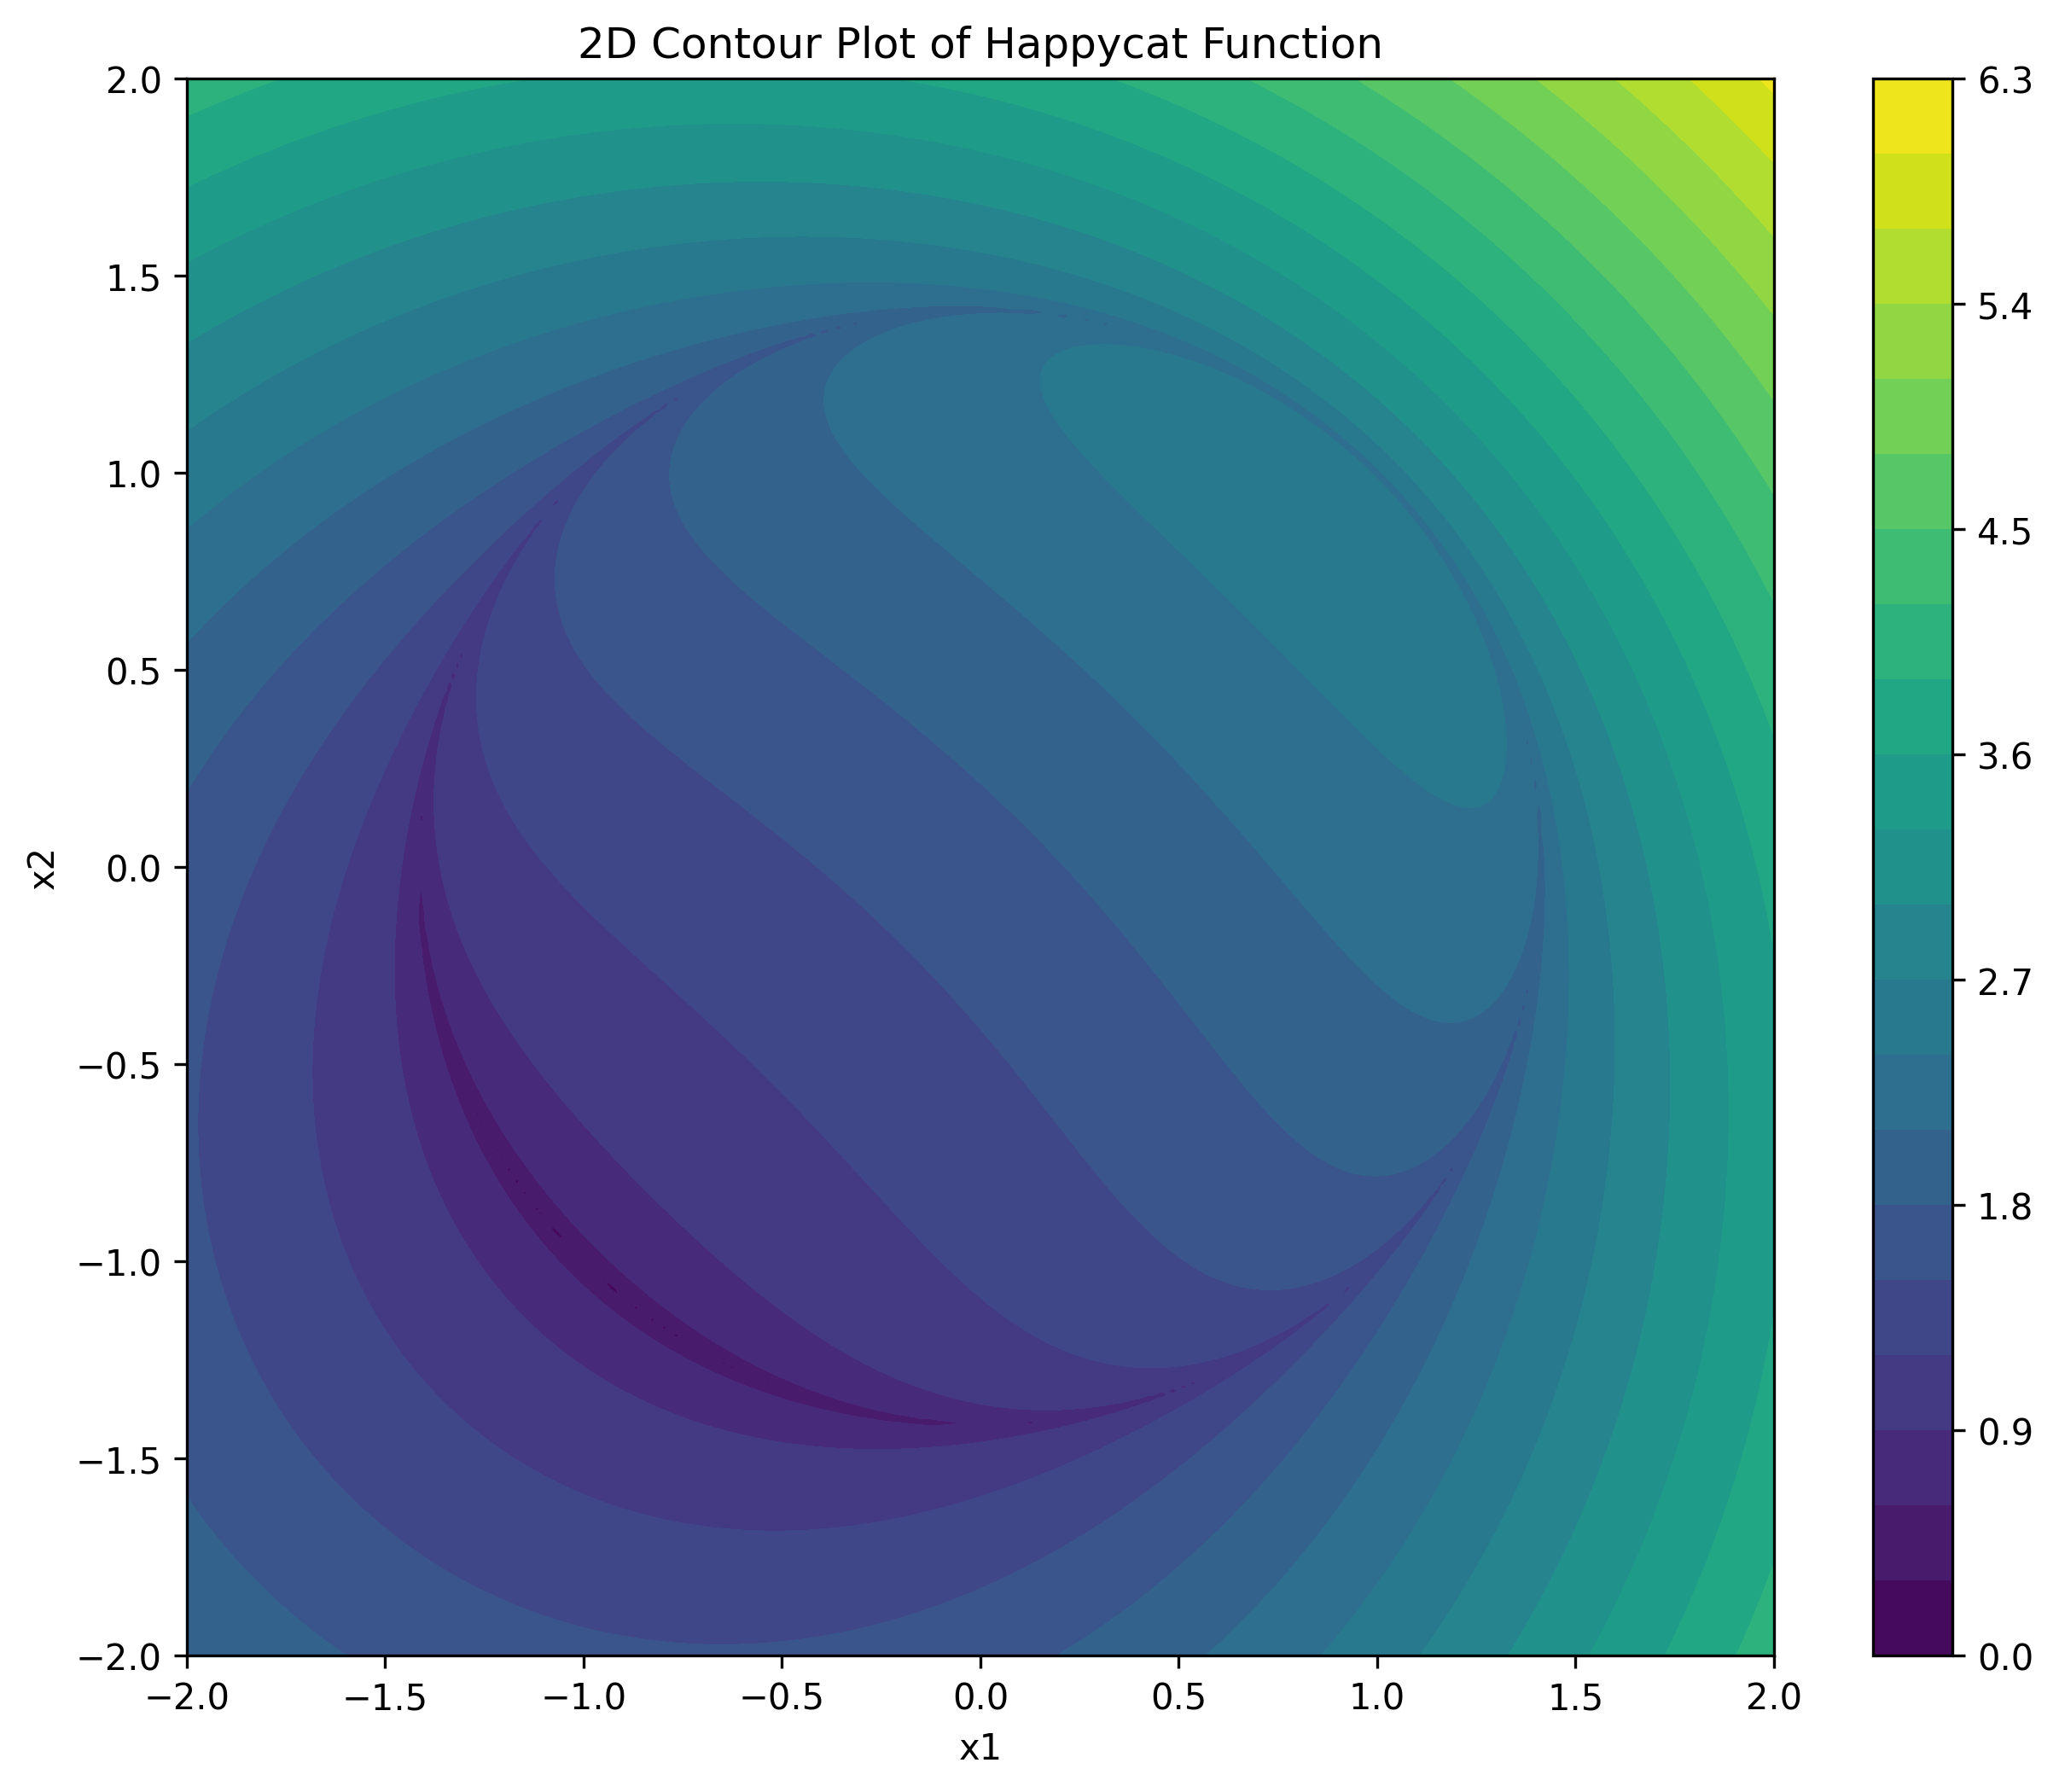
\includegraphics[width=\linewidth]{cec/happycat_2d.png}
		\caption{Dimensi 2}
		\label{fig:happycat-2d}
	\end{subfigure}
	\hfill
	\begin{subfigure}[b]{0.4\textwidth}
		\centering
		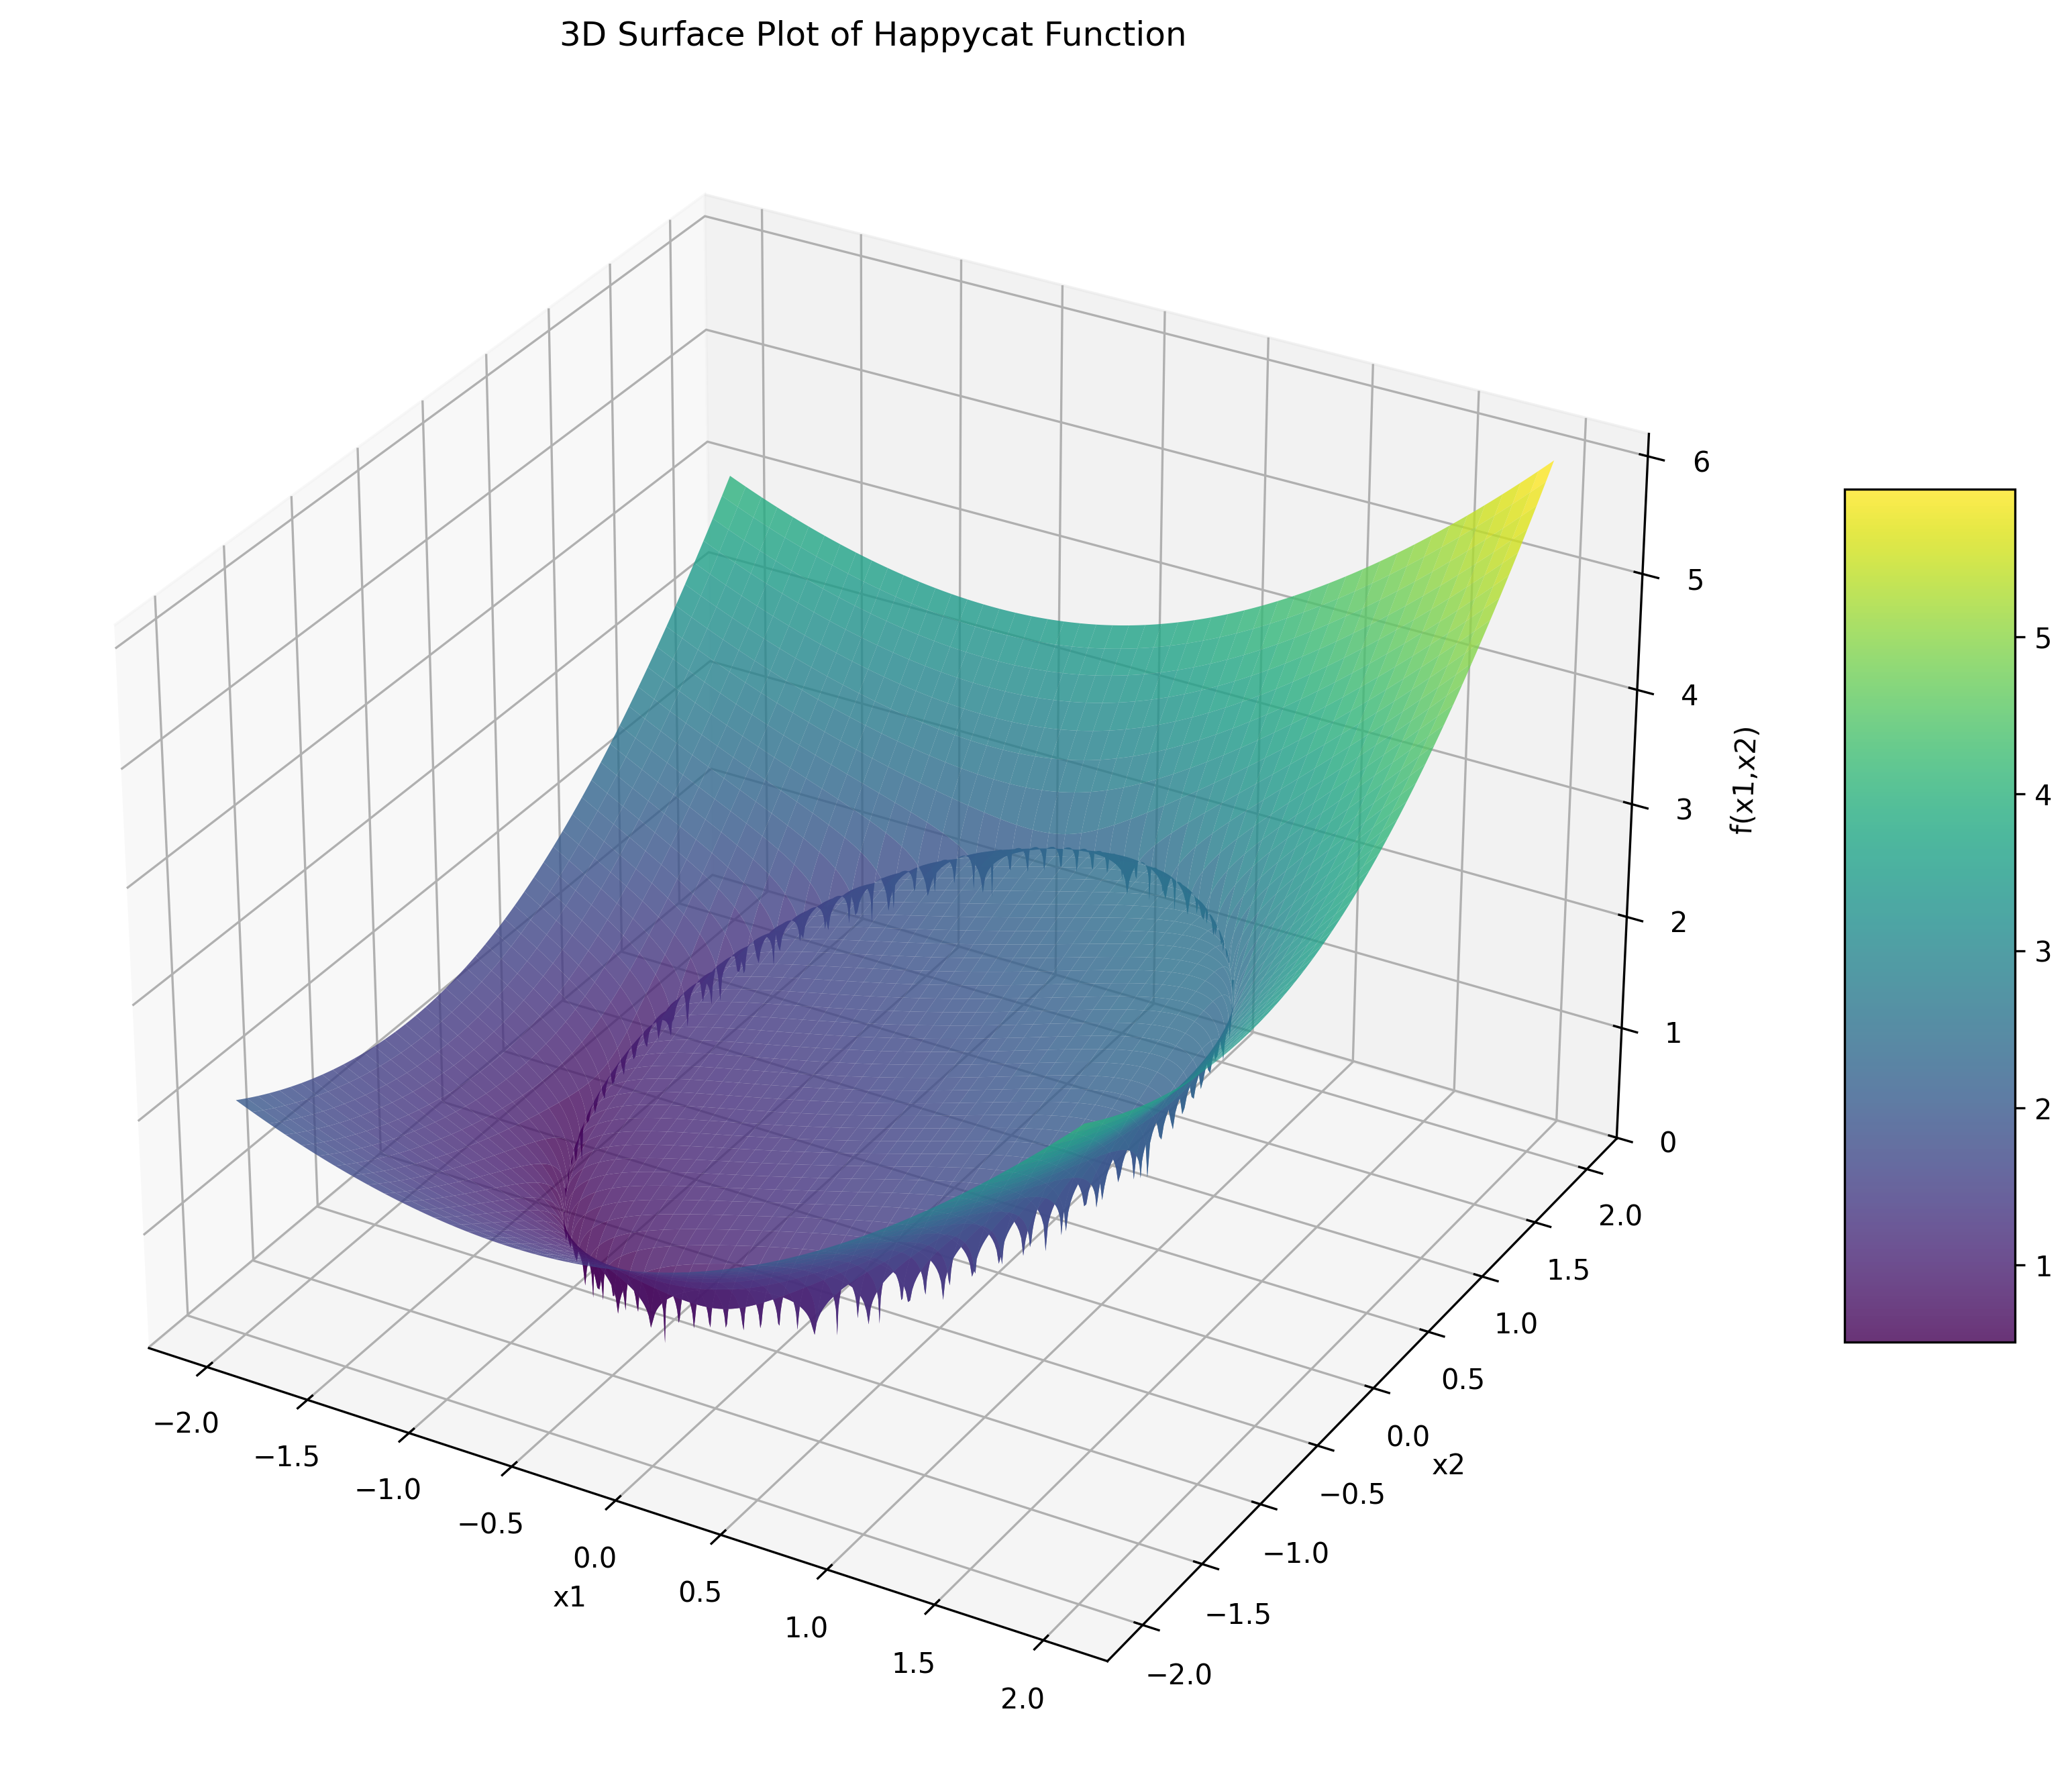
\includegraphics[width=\linewidth]{cec/happycat_3d.png}
		\caption{Dimensi 3}
		\label{fig:happycat-3d}
	\end{subfigure}
	\caption{Tampilan grafik fungsi Happycat pada dimensi dua (\cref{fig:happycat-2d}) dan tiga (\cref{fig:happycat-3d})}
	\label{fig:happycat}
\end{figure}
\begin{flalign*}
  f_{\text{Happycat}}(\mathrm{x})=\left|\sum_{i=1}^{D}z_i^2-D \right|^{1/4}+\left(0.5\sum_{i=1}^{D}z_i+\sum_{i=1}^{D}z_i \right)/D+0.5+f_{\text{bias}}&&
\end{flalign*}

\subsubsection{HGbat}
\noindent Properti:
\begin{packed_item}
  \item multimodal
  \item non-convex
  \item non-separable
\end{packed_item}
\begin{figure}[H]
	\centering
	\begin{subfigure}[b]{0.4\textwidth}
		\centering
		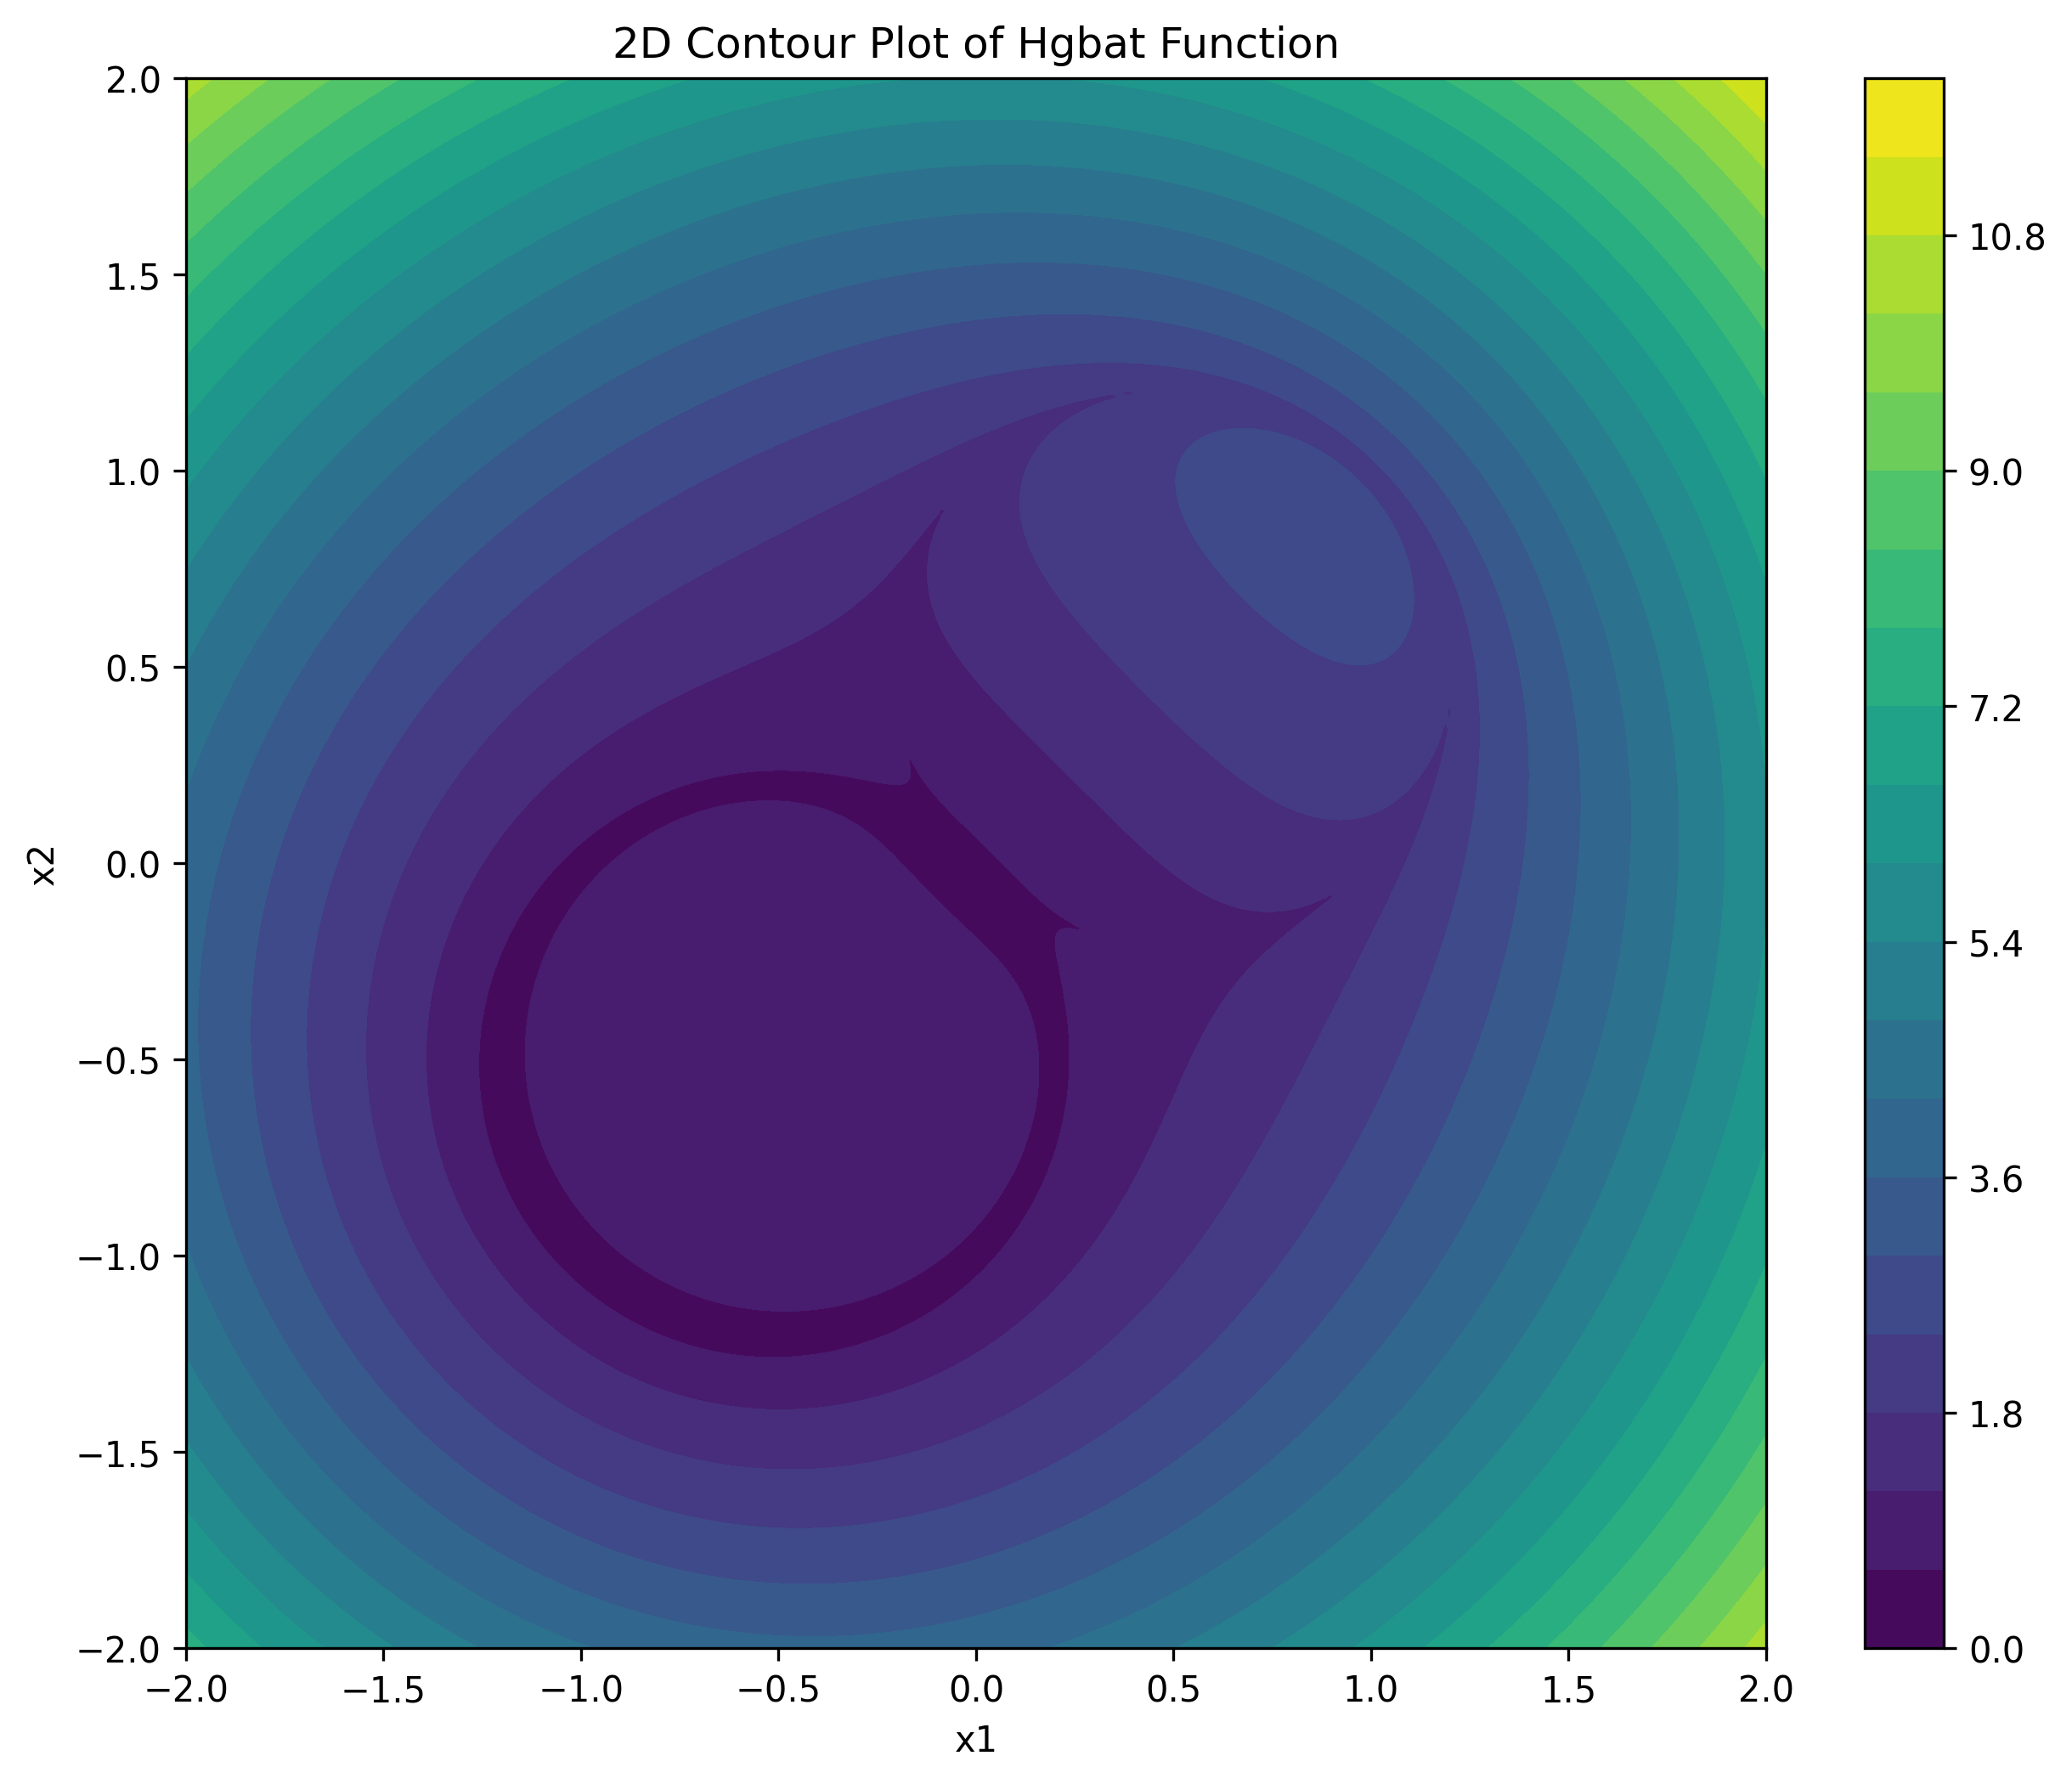
\includegraphics[width=\linewidth]{cec/hgbat_2d.png}
		\caption{Dimensi 2}
		\label{fig:hgbat-2d}
	\end{subfigure}
	\hfill
	\begin{subfigure}[b]{0.4\textwidth}
		\centering
		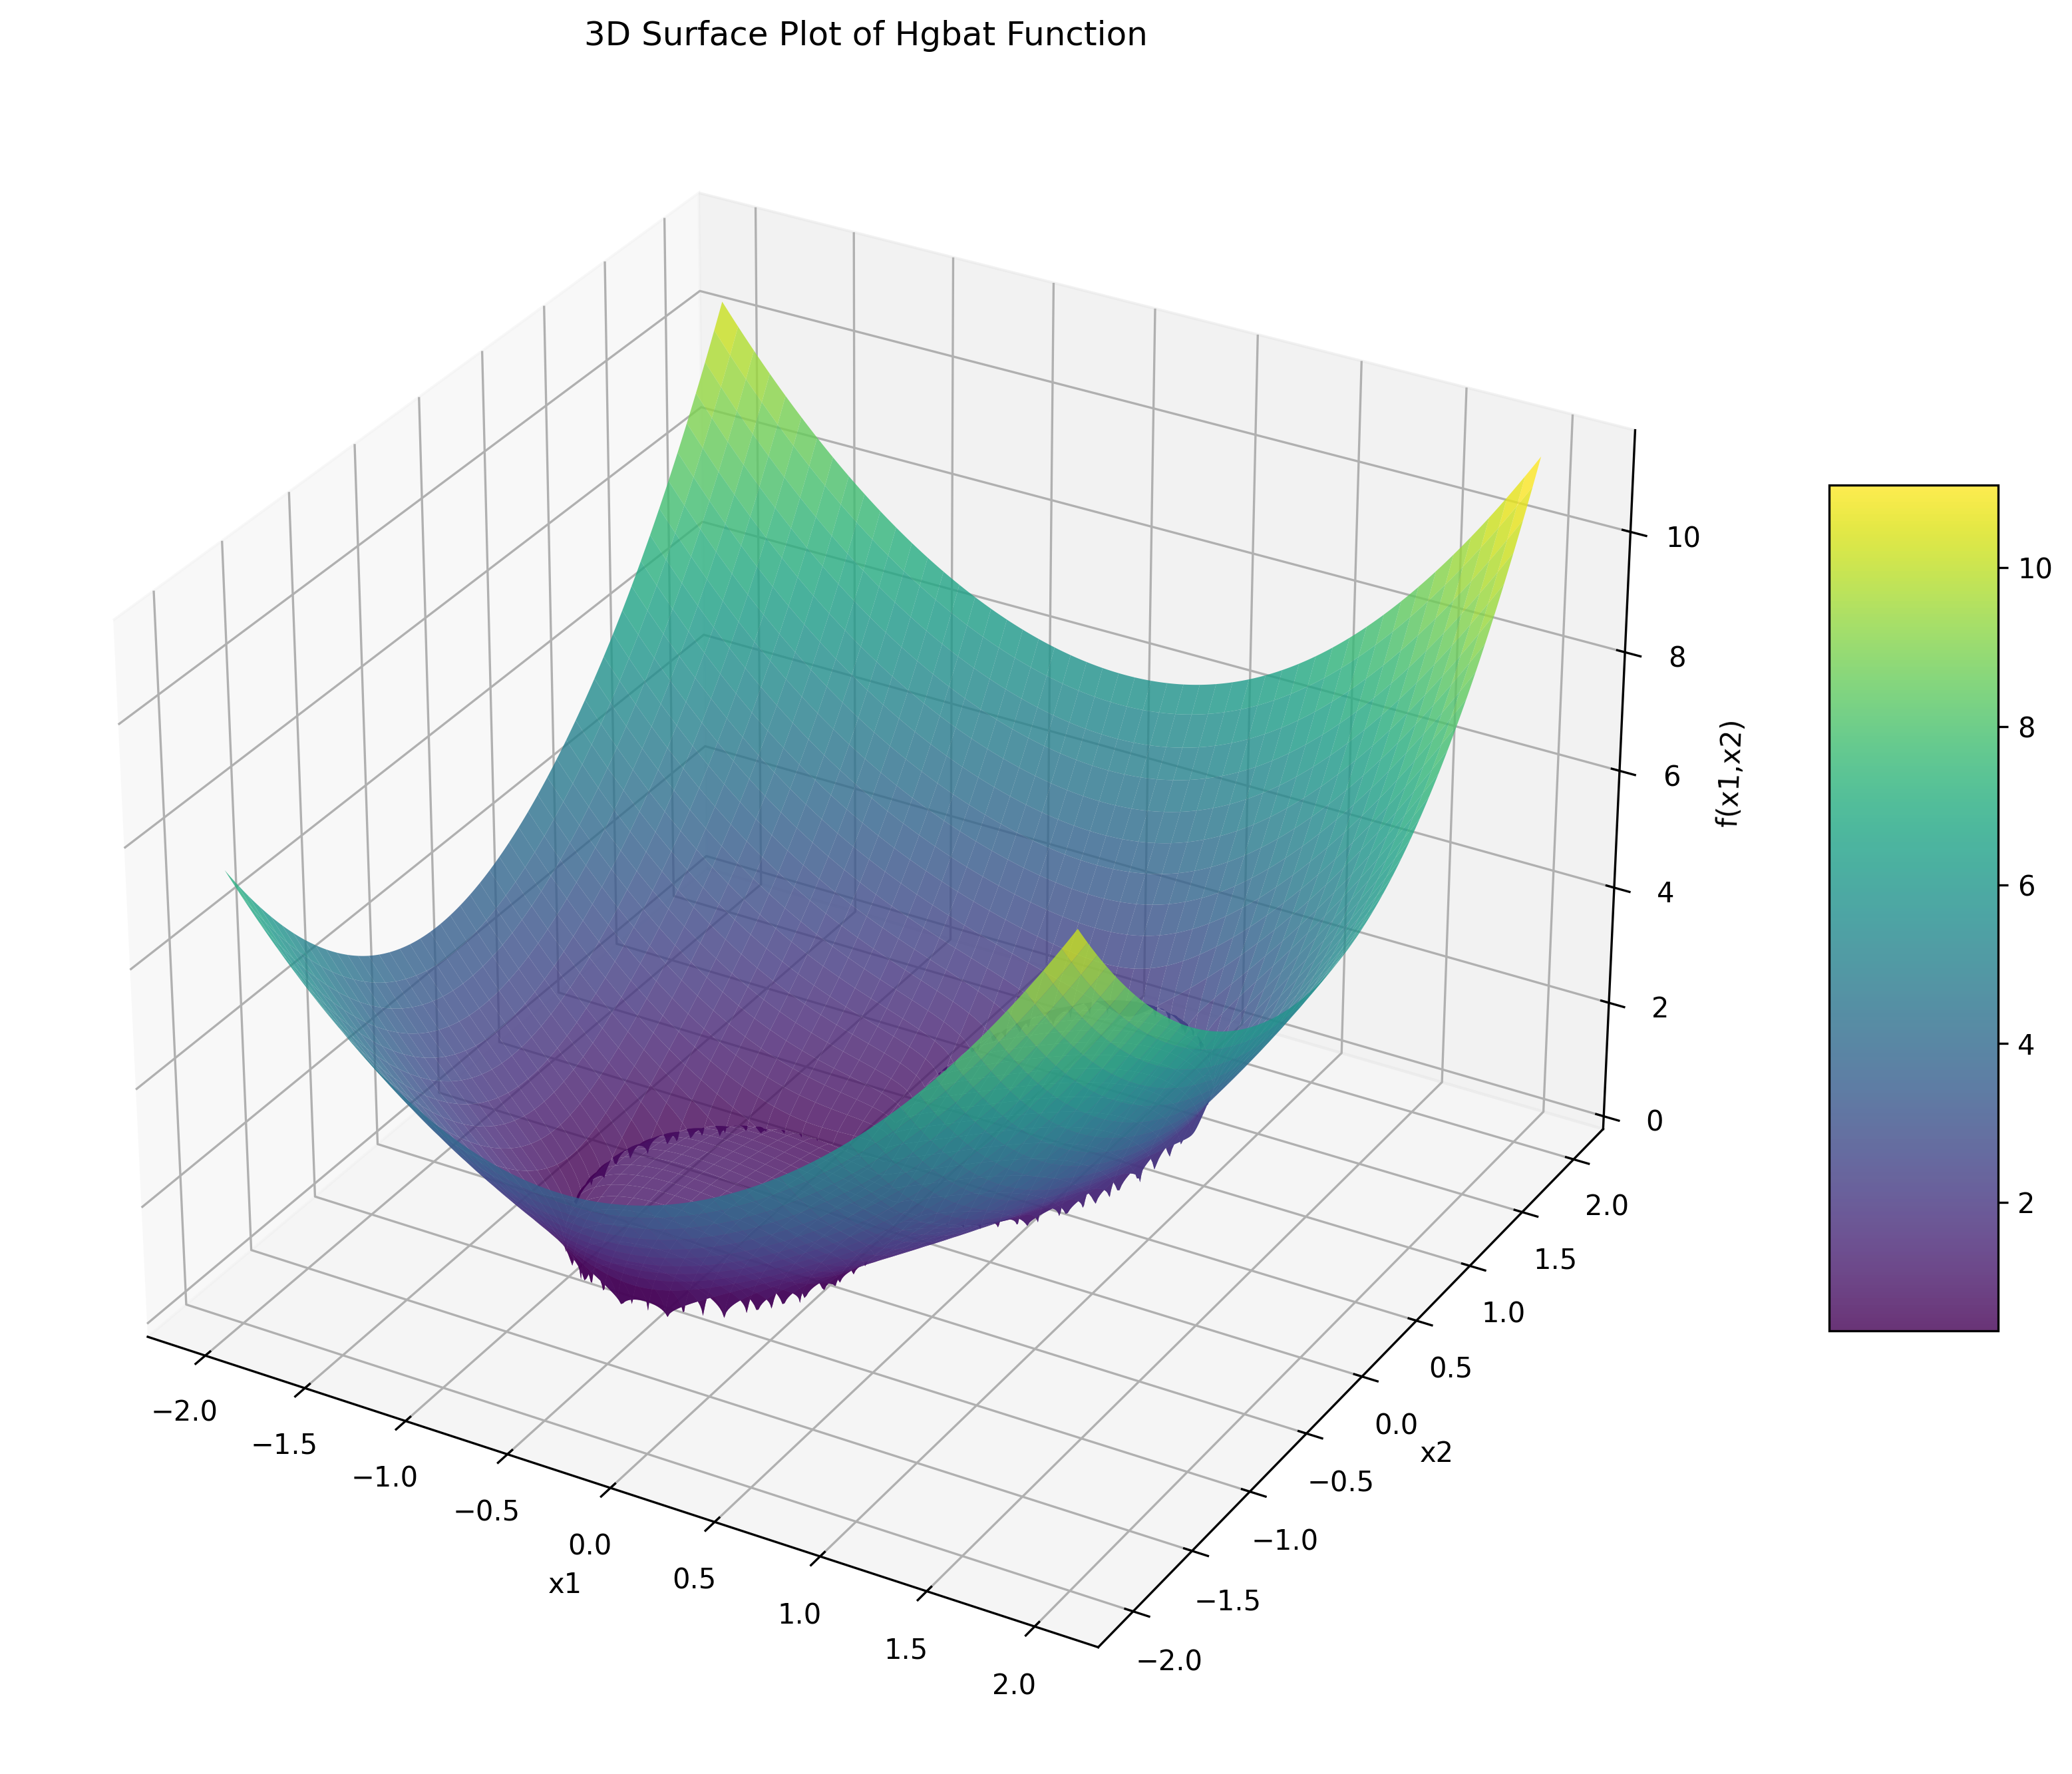
\includegraphics[width=\linewidth]{cec/hgbat_3d.png}
		\caption{Dimensi 3}
		\label{fig:hgbat-3d}
	\end{subfigure}
	\caption{Tampilan grafik fungsi HGbat pada dimensi dua (\cref{fig:hgbat-2d}) dan tiga (\cref{fig:hgbat-3d})}
	\label{fig:hgbat}
\end{figure}
\begin{flalign*}
  f_{\text{HGbat}}(\mathrm{x})=\left|\left( \sum_{i=1}^{D}z_i^2\right)^2-\left(\sum_{i=1}^{D}z_i \right)^2  \right|^{1/2}+\left(0.5\sum_{i=1}^{D}z_i+\sum_{i=1}^{D}z_i \right)/D+0.5+f_{\text{bias}}&&
\end{flalign*}

\subsubsection{Katsuura}
\noindent Properti:
\begin{packed_item}
  \item multimodal
  \item non-convex
  \item non-separable
  \item Continuous everywhere yet differentiable nowhere
\end{packed_item}
\begin{figure}[H]
	\centering
	\begin{subfigure}[b]{0.4\textwidth}
		\centering
		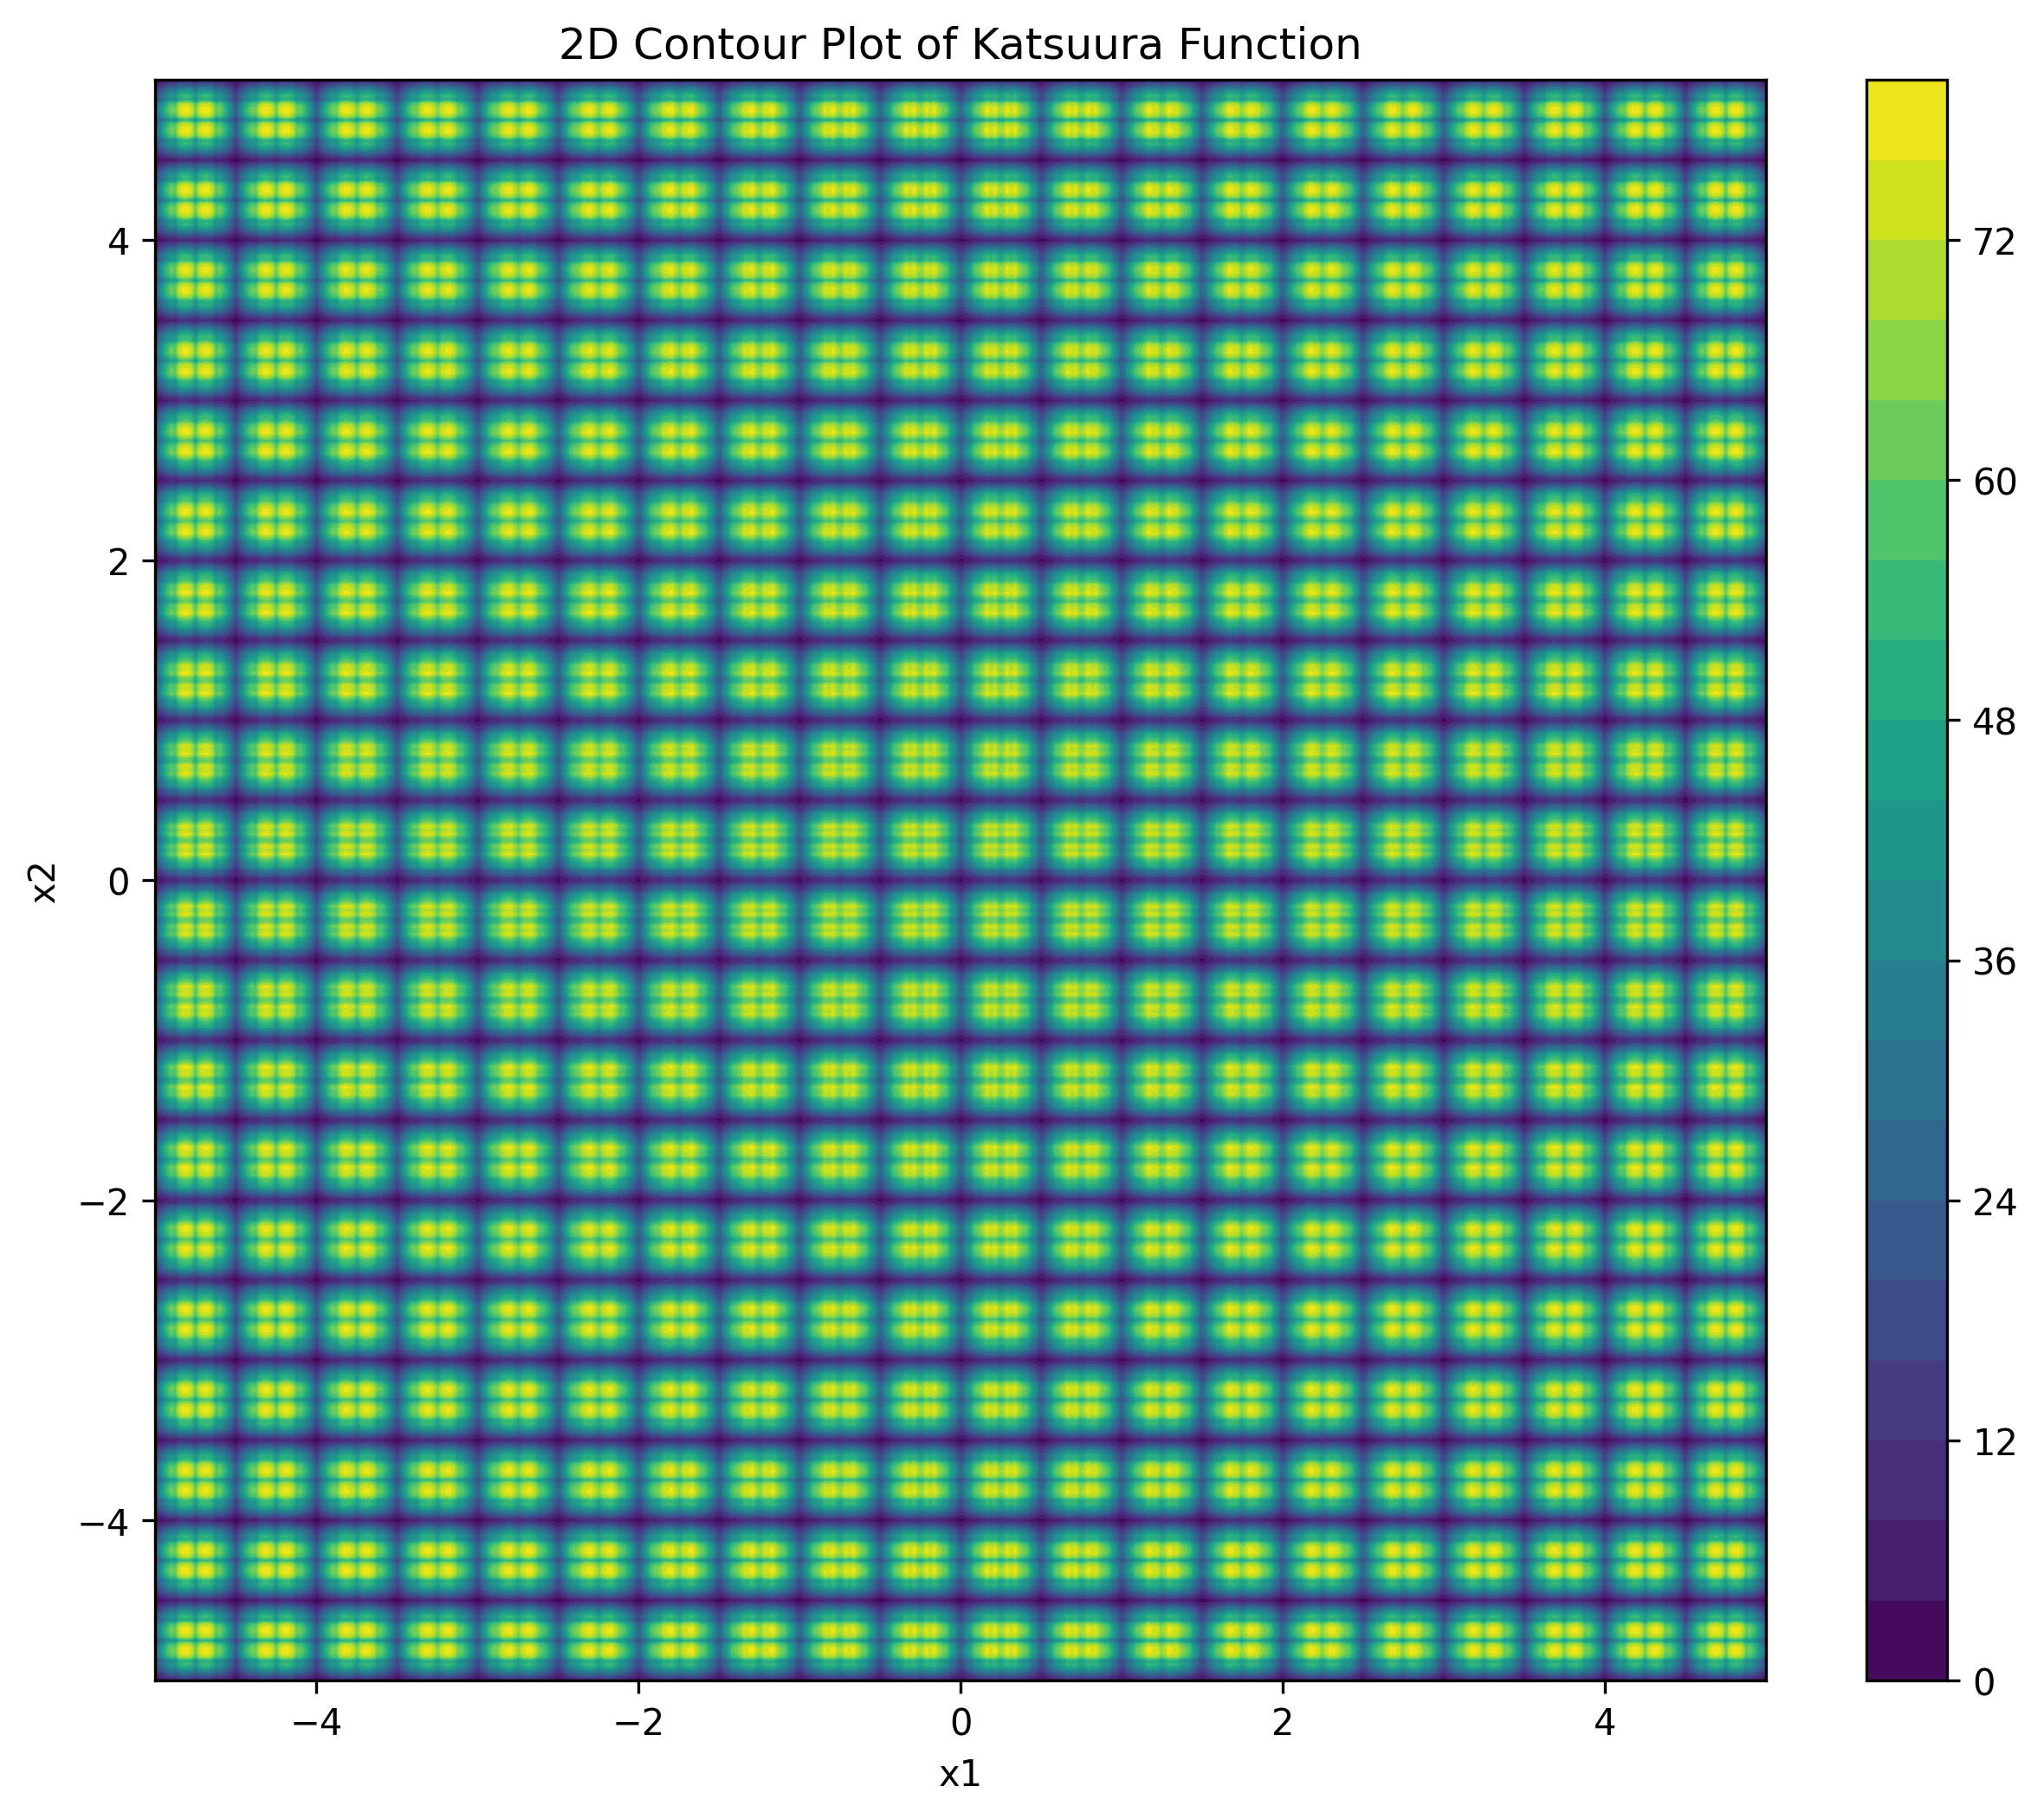
\includegraphics[width=\linewidth]{cec/katsuura_2d.png}
		\caption{Dimensi 2}
		\label{fig:katsuura-2d}
	\end{subfigure}
	\hfill
	\begin{subfigure}[b]{0.4\textwidth}
		\centering
		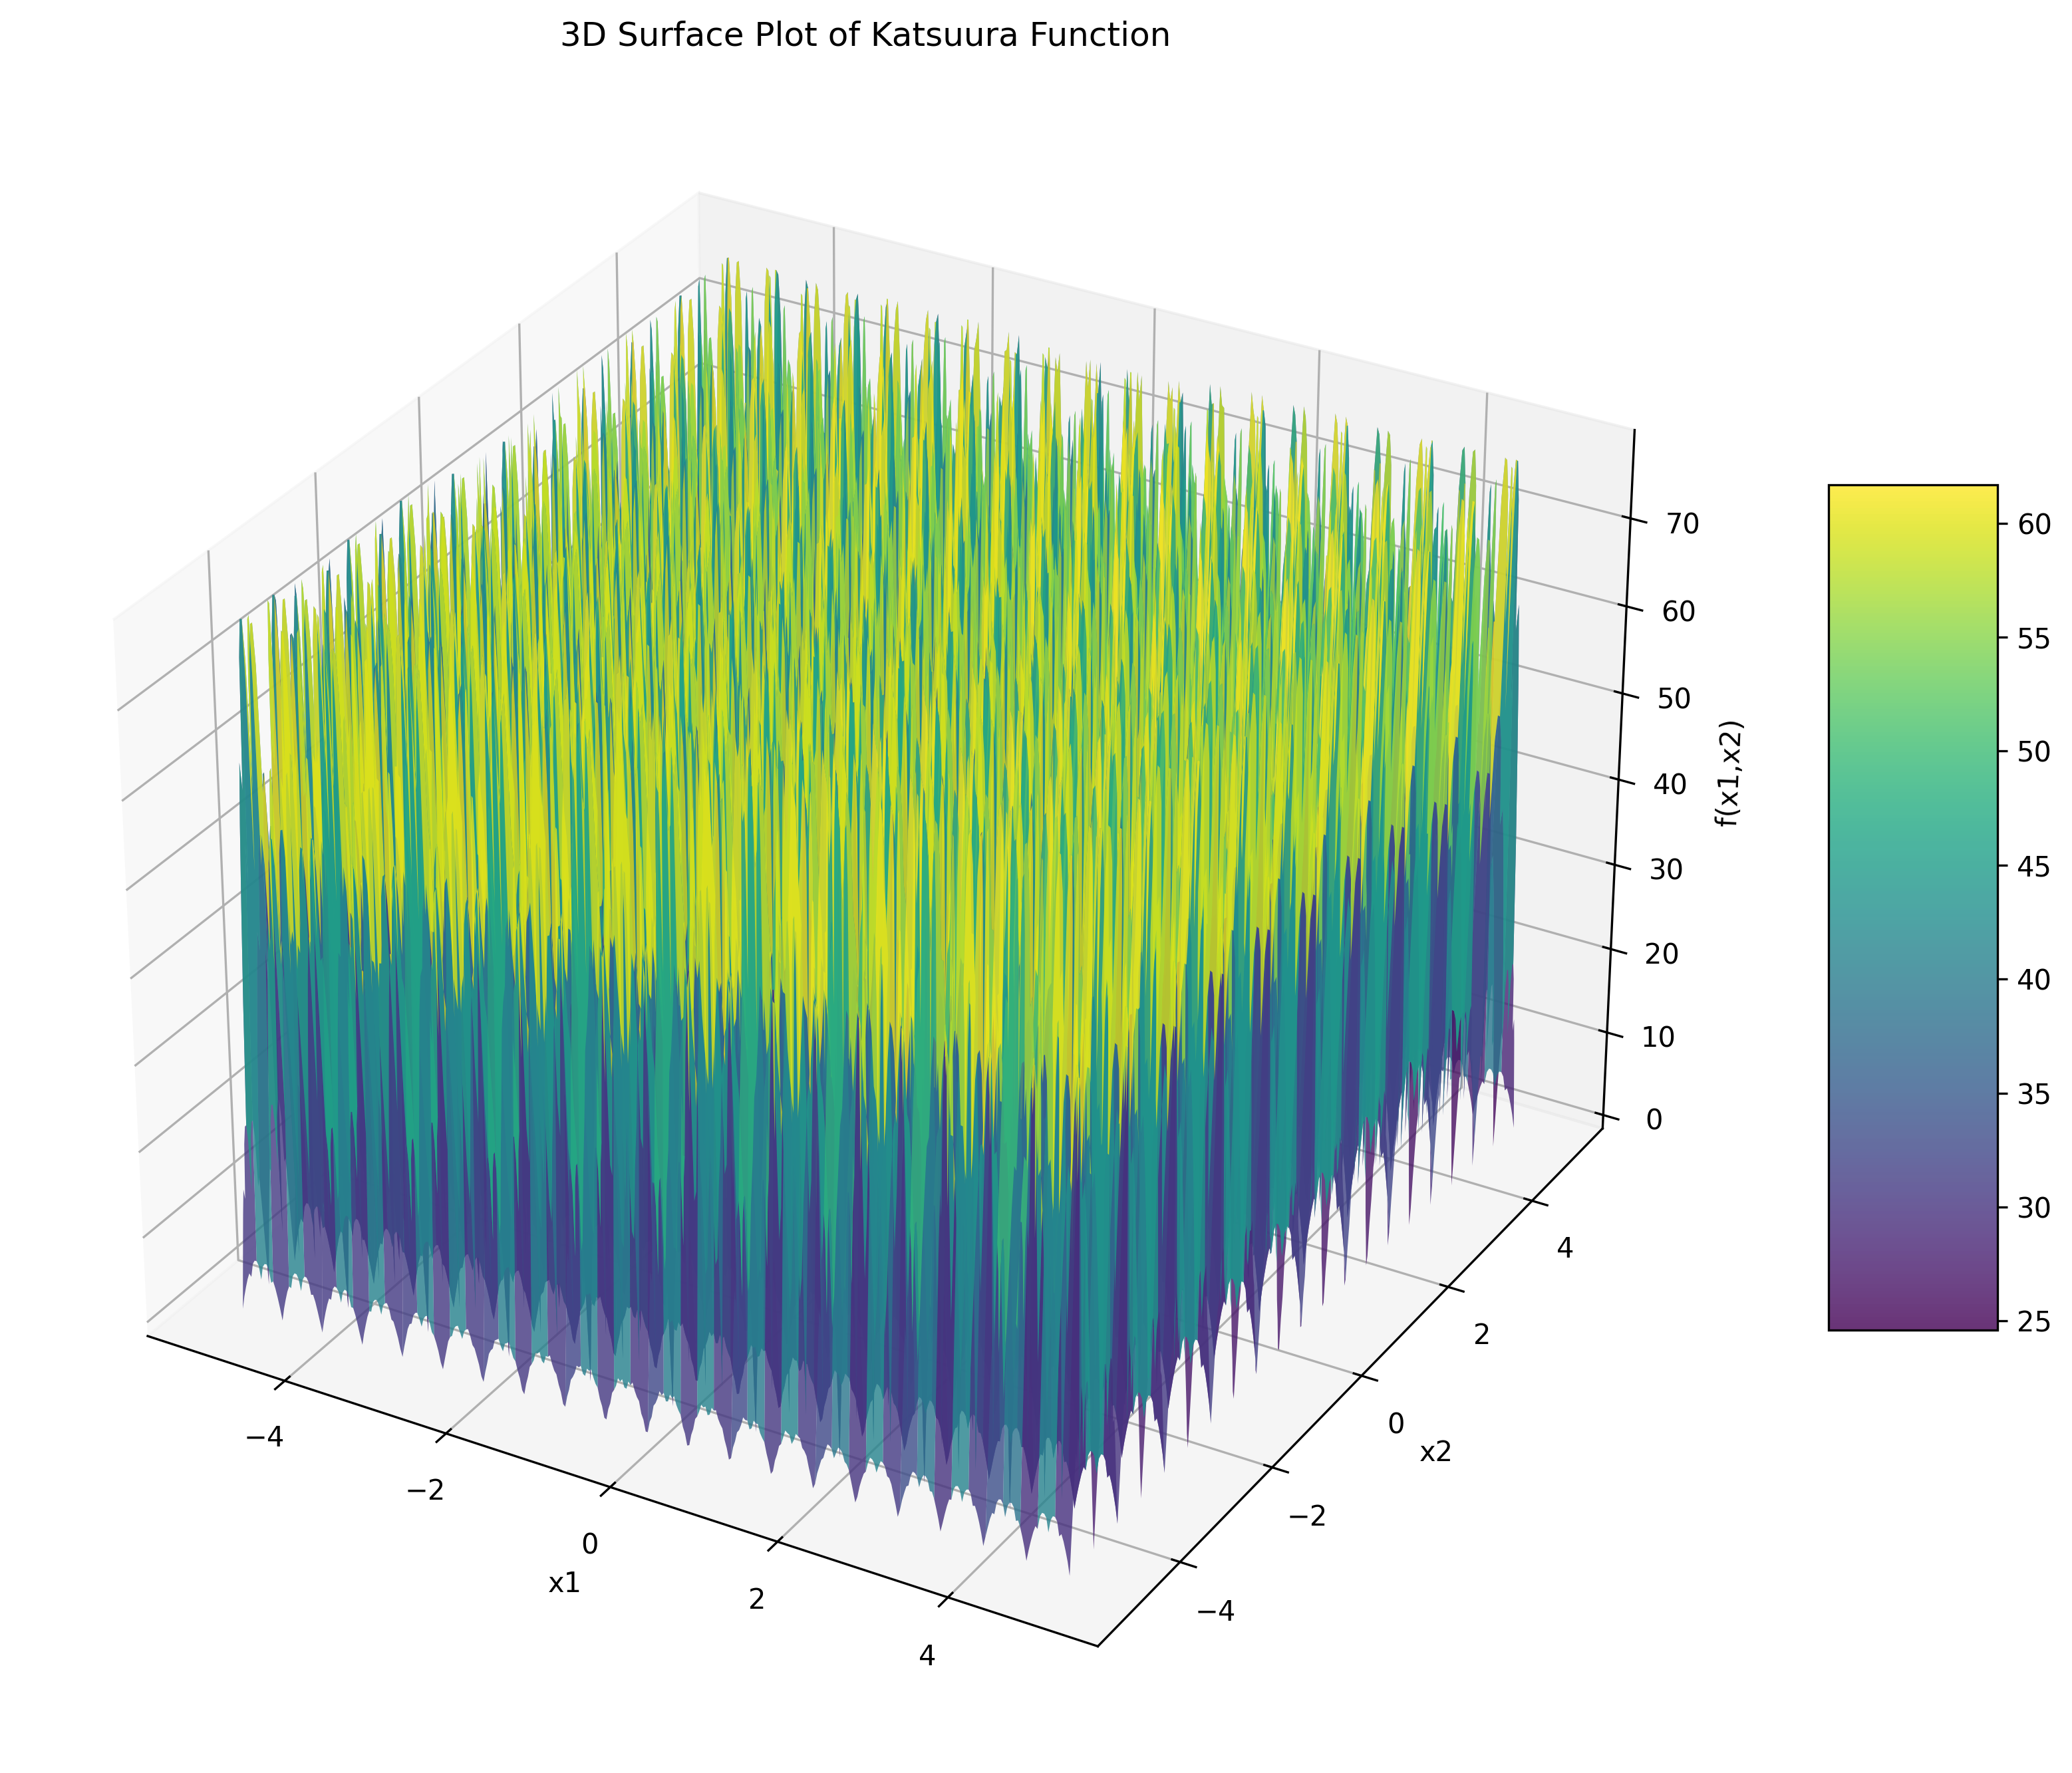
\includegraphics[width=\linewidth]{cec/katsuura_3d.png}
		\caption{Dimensi 3}
		\label{fig:katsuura-3d}
	\end{subfigure}
	\caption{Tampilan grafik fungsi Katsuura pada dimensi dua (\cref{fig:katsuura-2d}) dan tiga (\cref{fig:katsuura-3d})}
	\label{fig:katsuura}
\end{figure}
\begin{flalign*}
  f_{\text{Katsuura}}(\mathrm{x})=\frac{10}{D^2}\prod_{i=1}^{D}\left( 1+i\sum_{j=1}^{32}\frac{\left|2^j z_i-\text{round}\left( 2^jz_i\right)  \right| }{2^j}\right)^{\frac{10}{D^{1.2}}}+f_{\text{bias}}&&
\end{flalign*}

\subsubsection{Levy}
\noindent Properti:
\begin{packed_item}
  \item multimodal
  \item non-convex
  \item non-separable
  \item Local optima's number is huge
\end{packed_item}
\begin{figure}[H]
	\centering
	\begin{subfigure}[b]{0.4\textwidth}
		\centering
		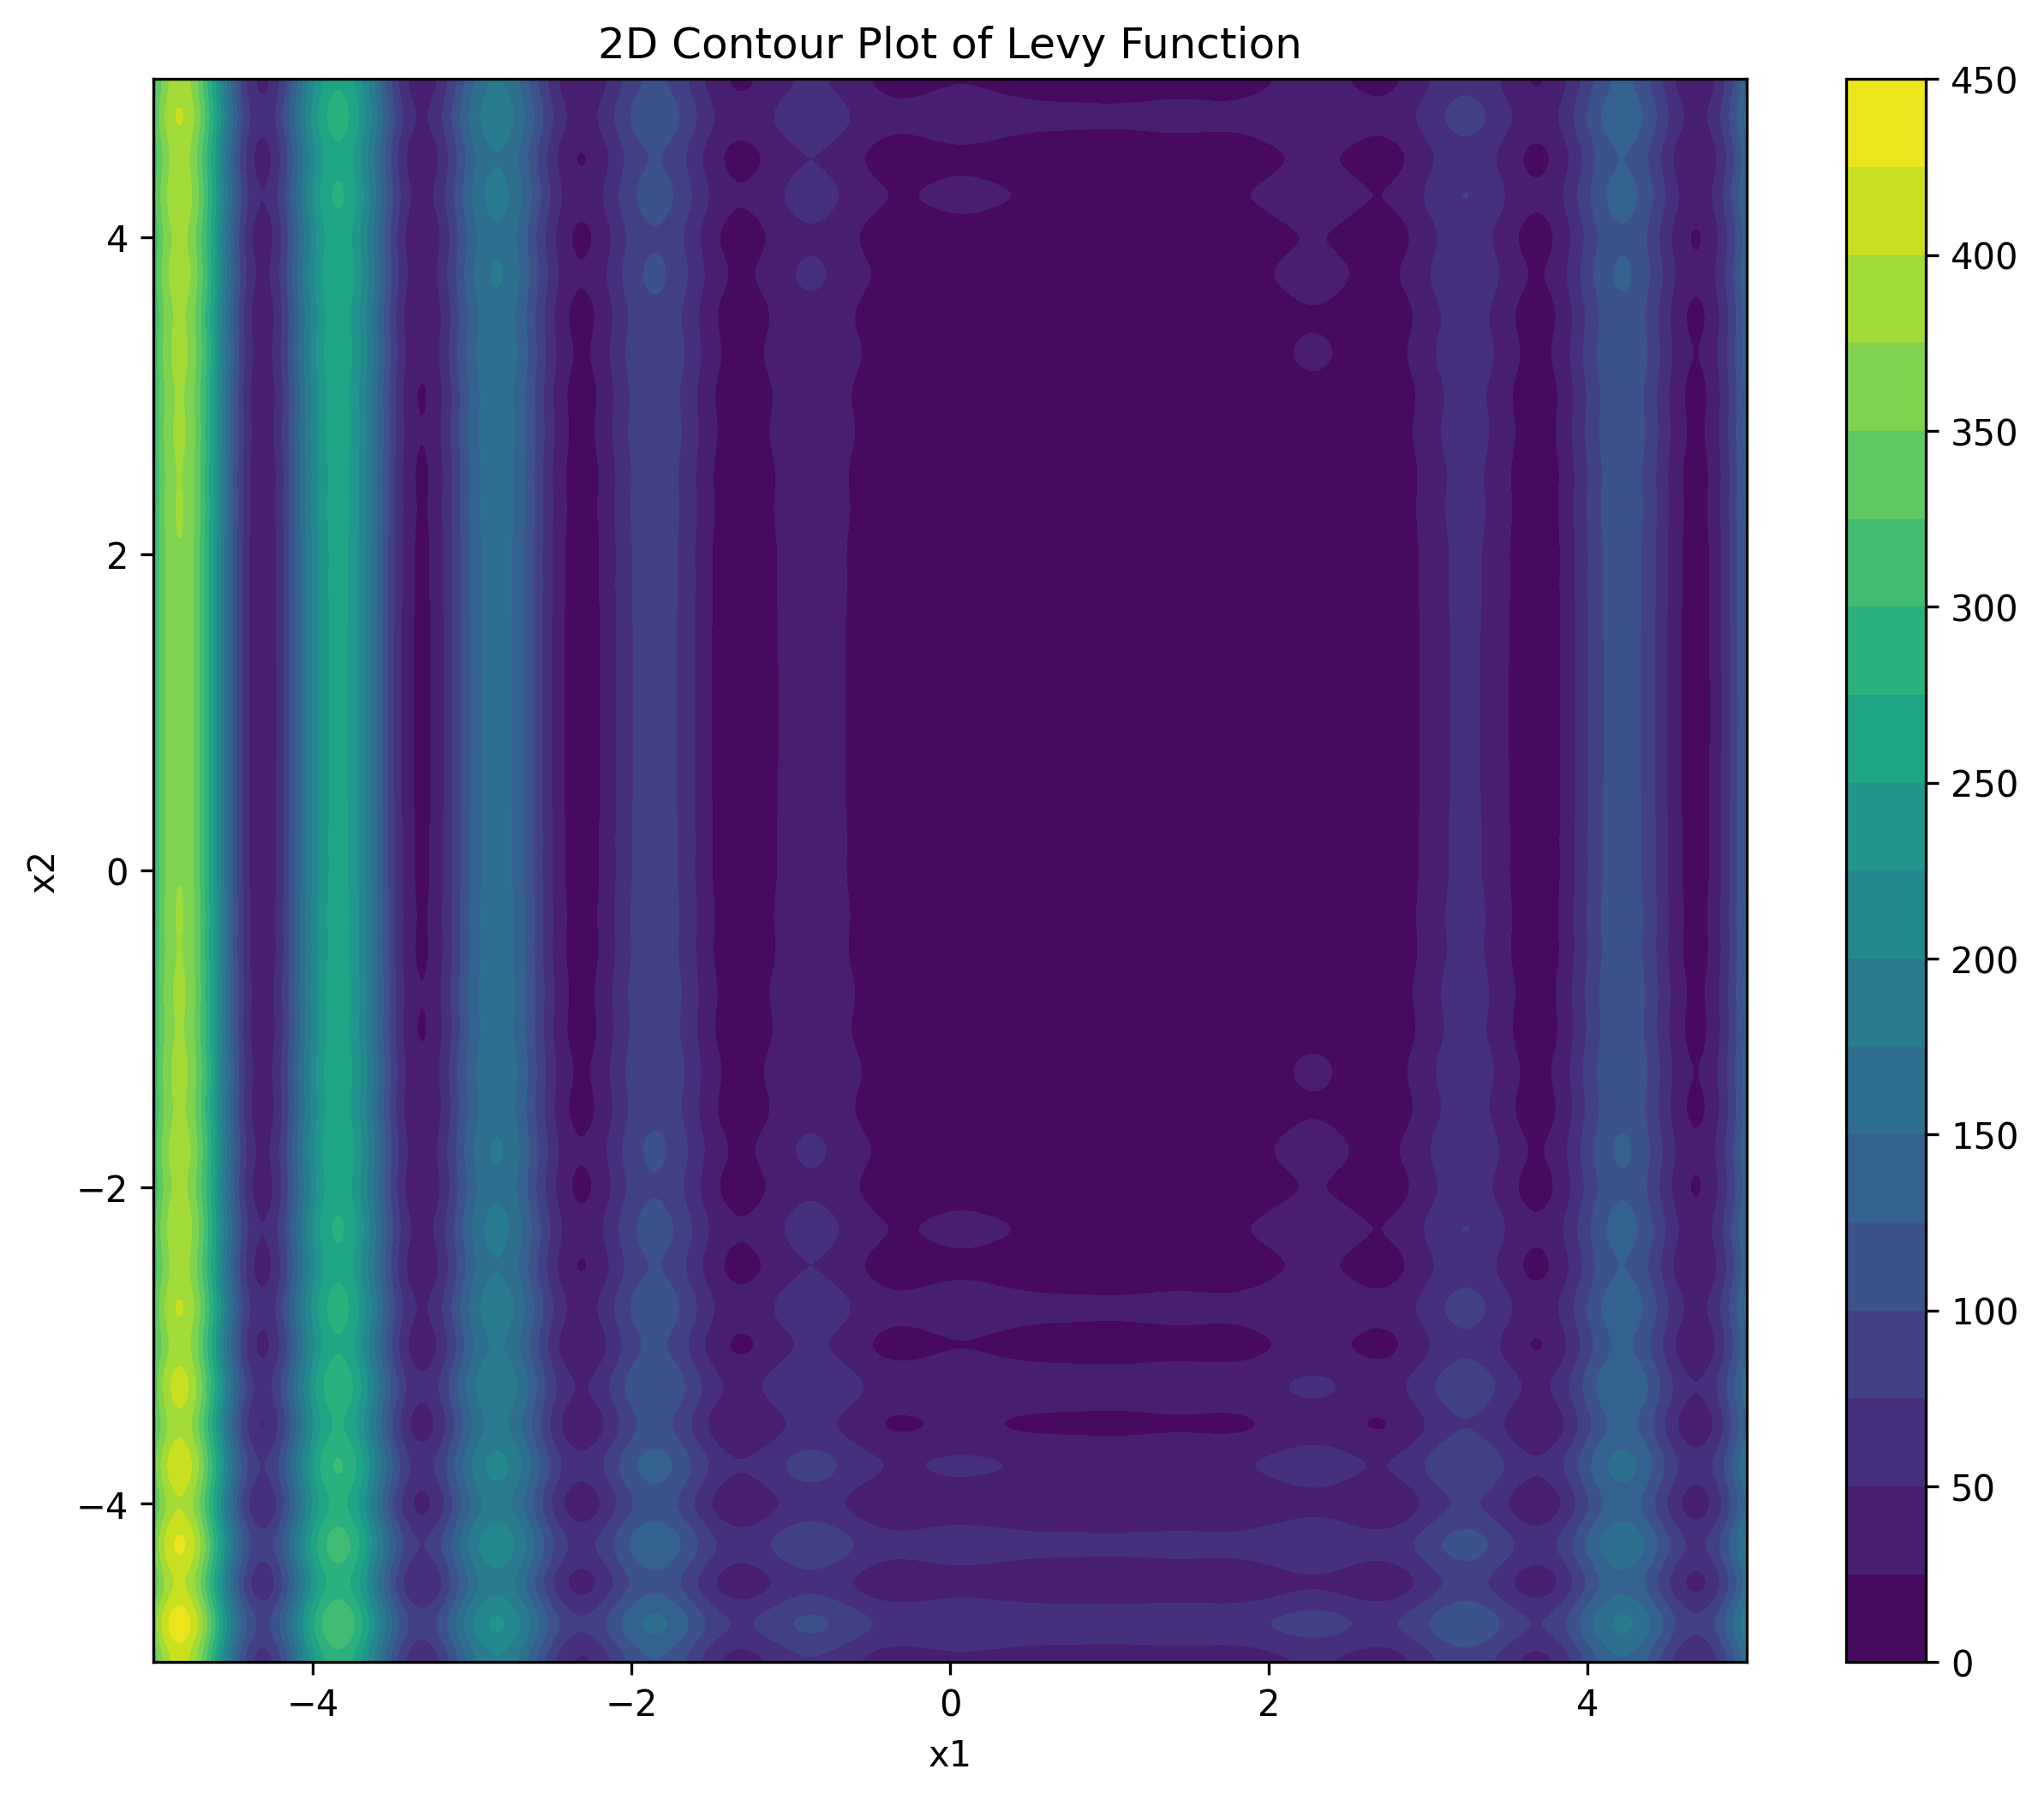
\includegraphics[width=\linewidth]{cec/levy_2d.png}
		\caption{Dimensi 2}
		\label{fig:levy-2d}
	\end{subfigure}
	\hfill
	\begin{subfigure}[b]{0.4\textwidth}
		\centering
		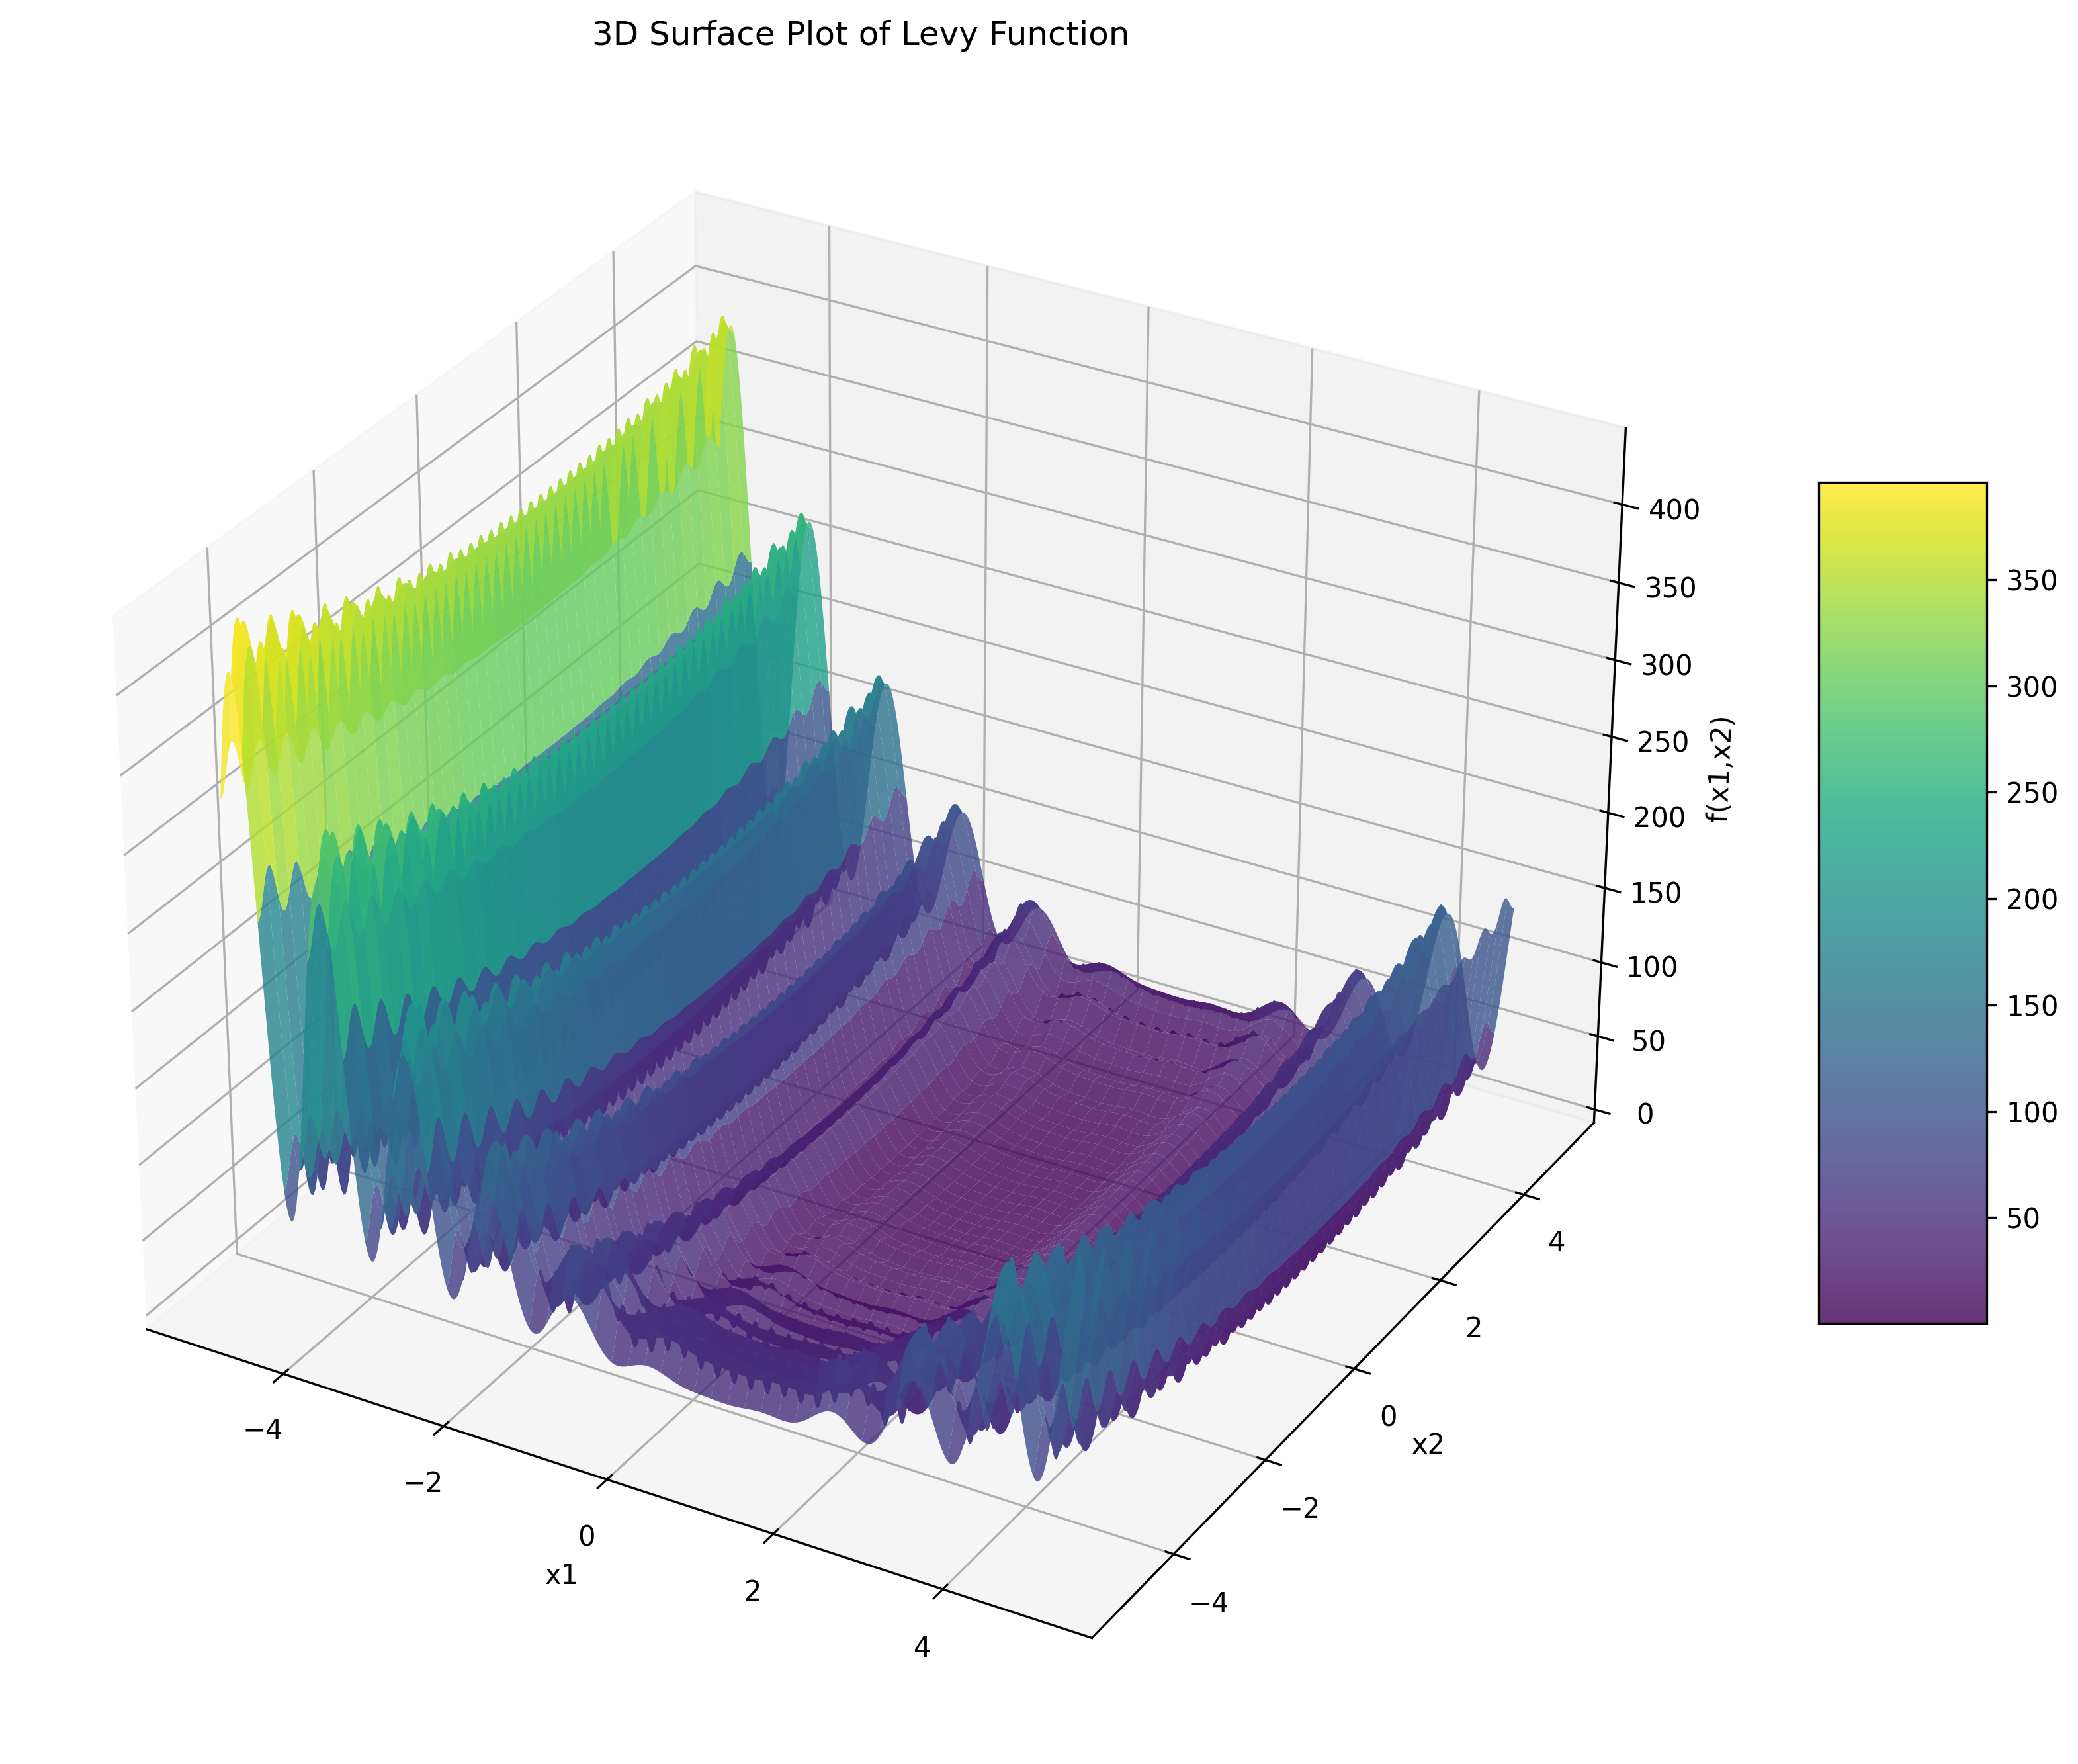
\includegraphics[width=\linewidth]{cec/levy_3d.png}
		\caption{Dimensi 3}
		\label{fig:levy-3d}
	\end{subfigure}
	\caption{Tampilan grafik fungsi Levy pada dimensi dua (\cref{fig:levy-2d}) dan tiga (\cref{fig:levy-3d})}
	\label{fig:levy}
\end{figure}
\begin{flalign*}
  &f_{\text{Levy}}(\mathrm{x})=\sin^2\left(\pi w_1 \right)+\sum_{i=1}^{D-1}\left(w_i-1 \right)^2\left[1+10\sin^2\left( \pi w_i+1\right)\right]+\left(w_D-1 \right)\left[1+\sin^2\left( 2\pi w_D\right)  \right]+f_{\text{bias}}&&\\
  &\text{dimana}\ w_i=1+\frac{z_i-1}{4},\forall i=1,\ldots,D&&
\end{flalign*}

\subsubsection{Rastrigin}
\noindent Properti:
\begin{packed_item}
  \item multimodal
  \item non-convex
  \item non-separable
  \item Local optima's number is huge
\end{packed_item}
\begin{figure}[H]
	\centering
	\begin{subfigure}[b]{0.4\textwidth}
		\centering
		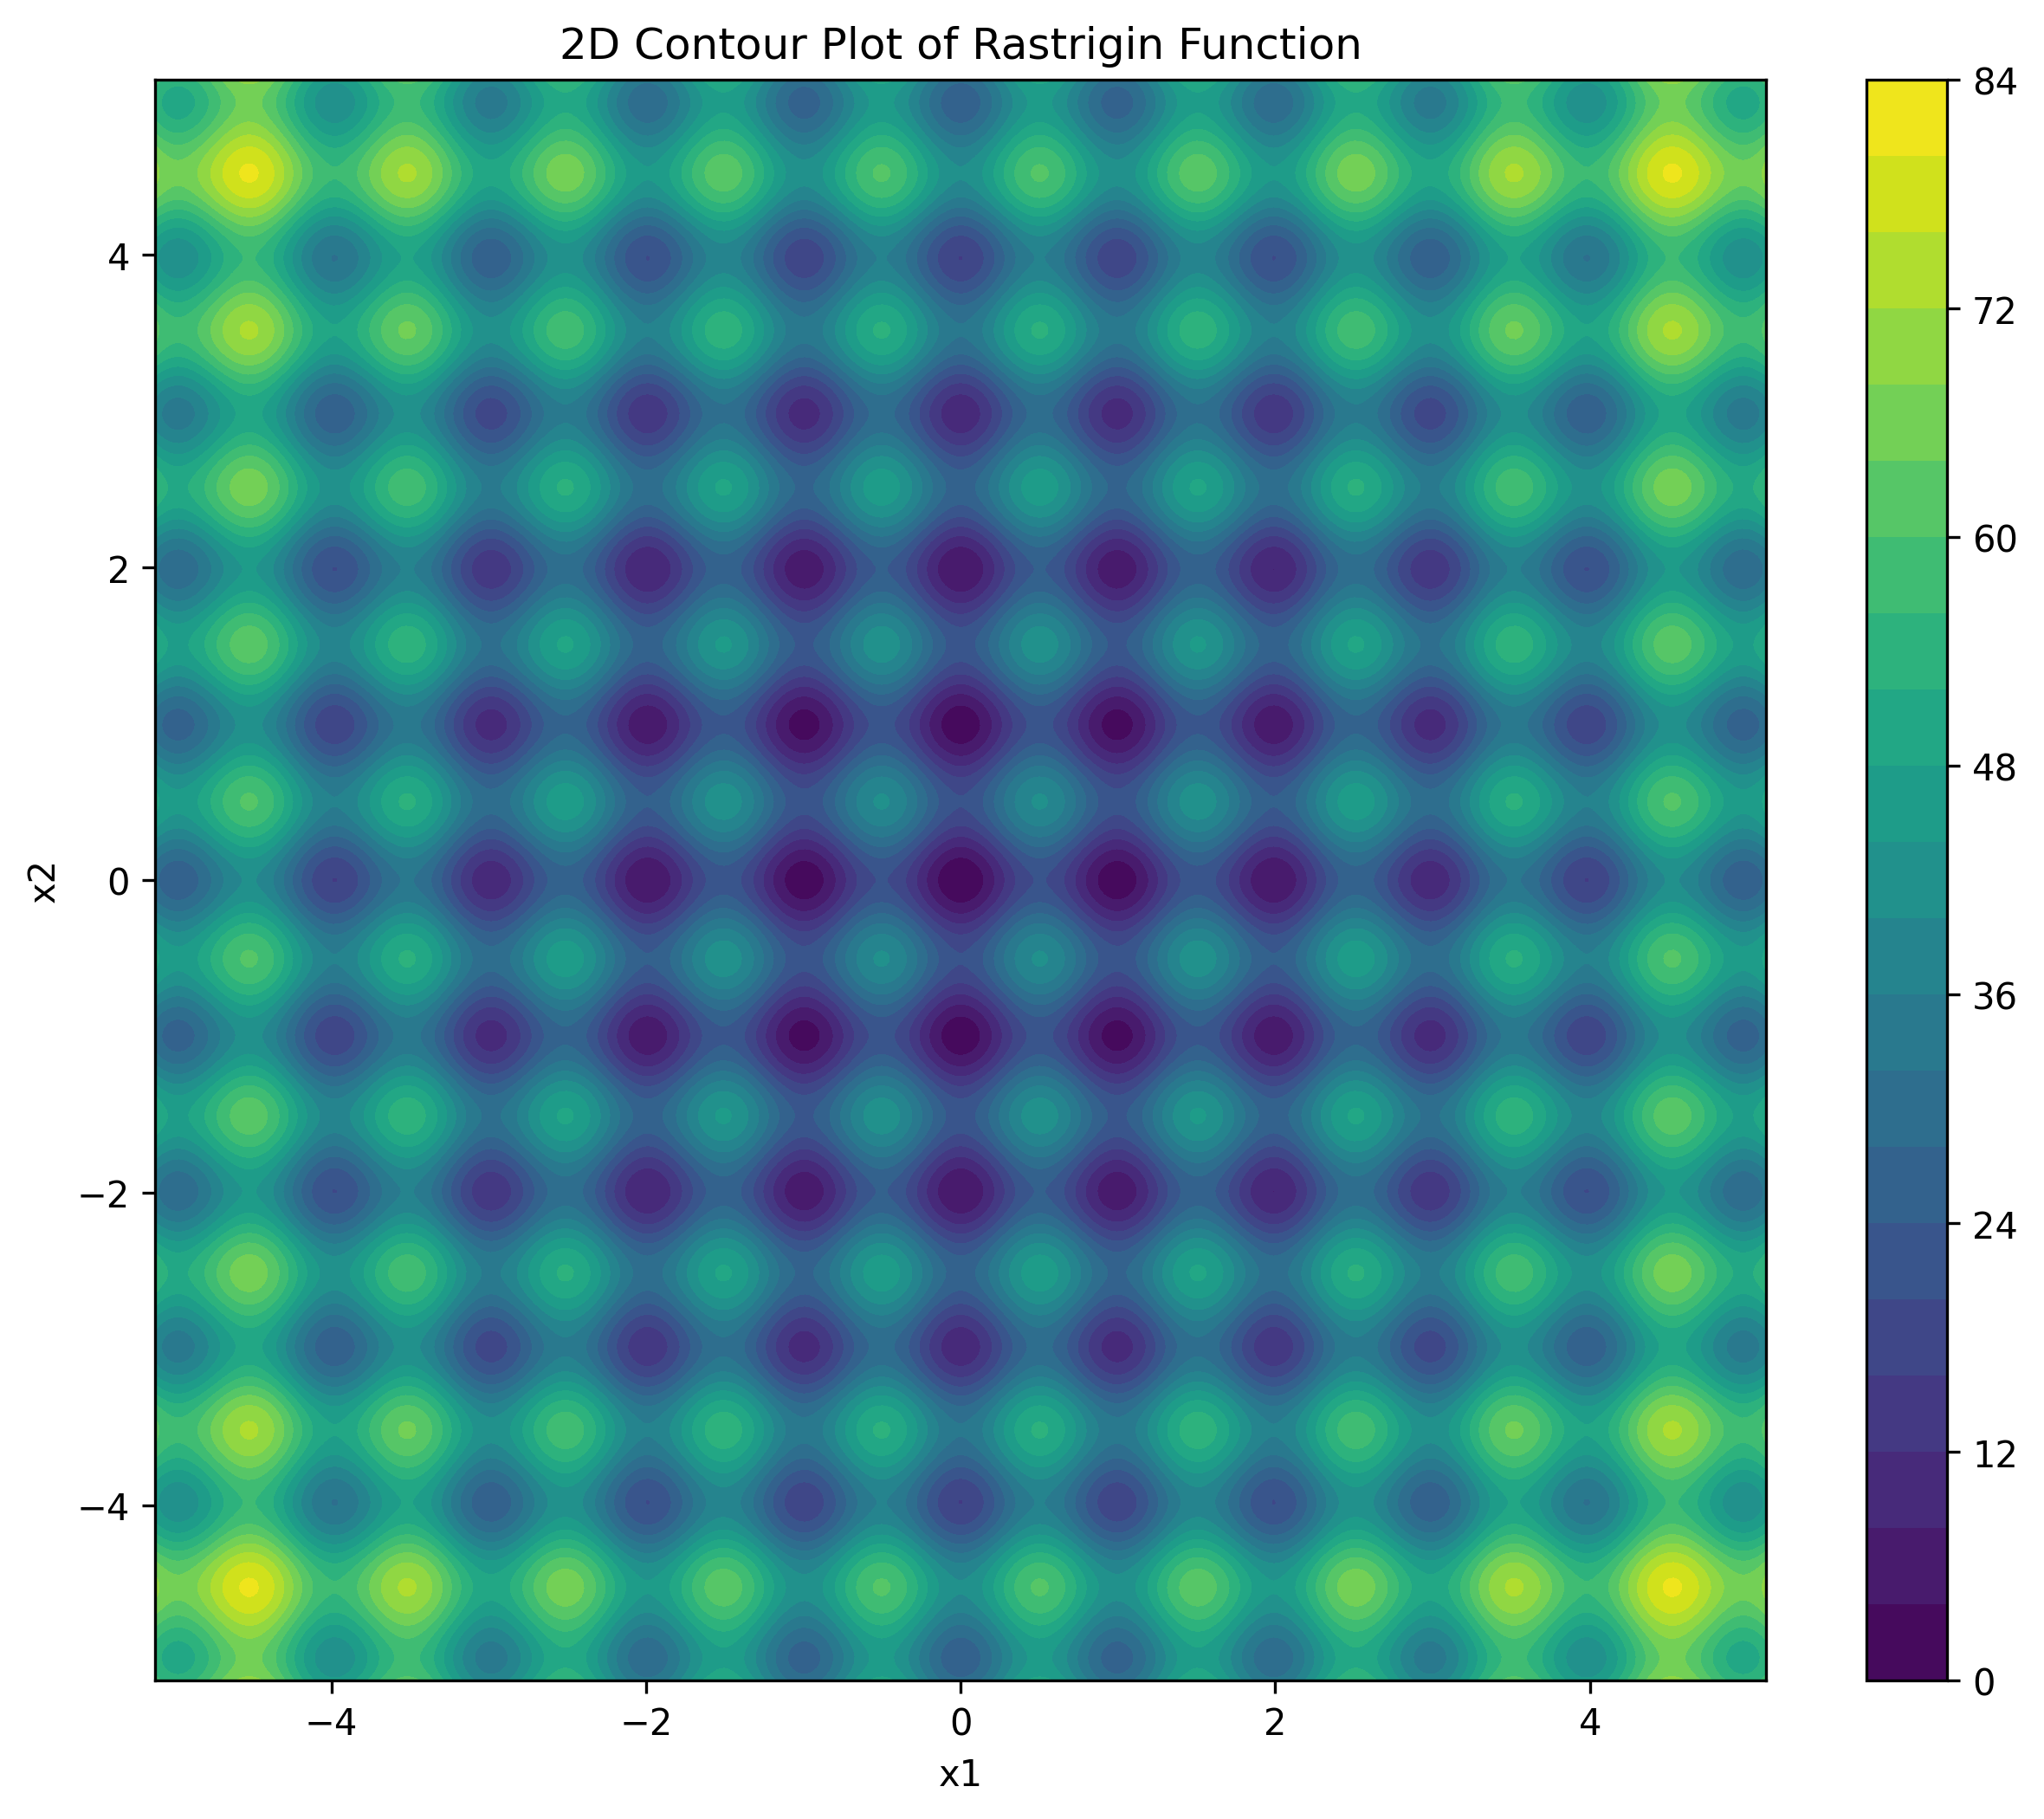
\includegraphics[width=\linewidth]{cec/rastrigin_2d.png}
		\caption{Dimensi 2}
		\label{fig:rastrigin-2d}
	\end{subfigure}
	\hfill
	\begin{subfigure}[b]{0.4\textwidth}
		\centering
		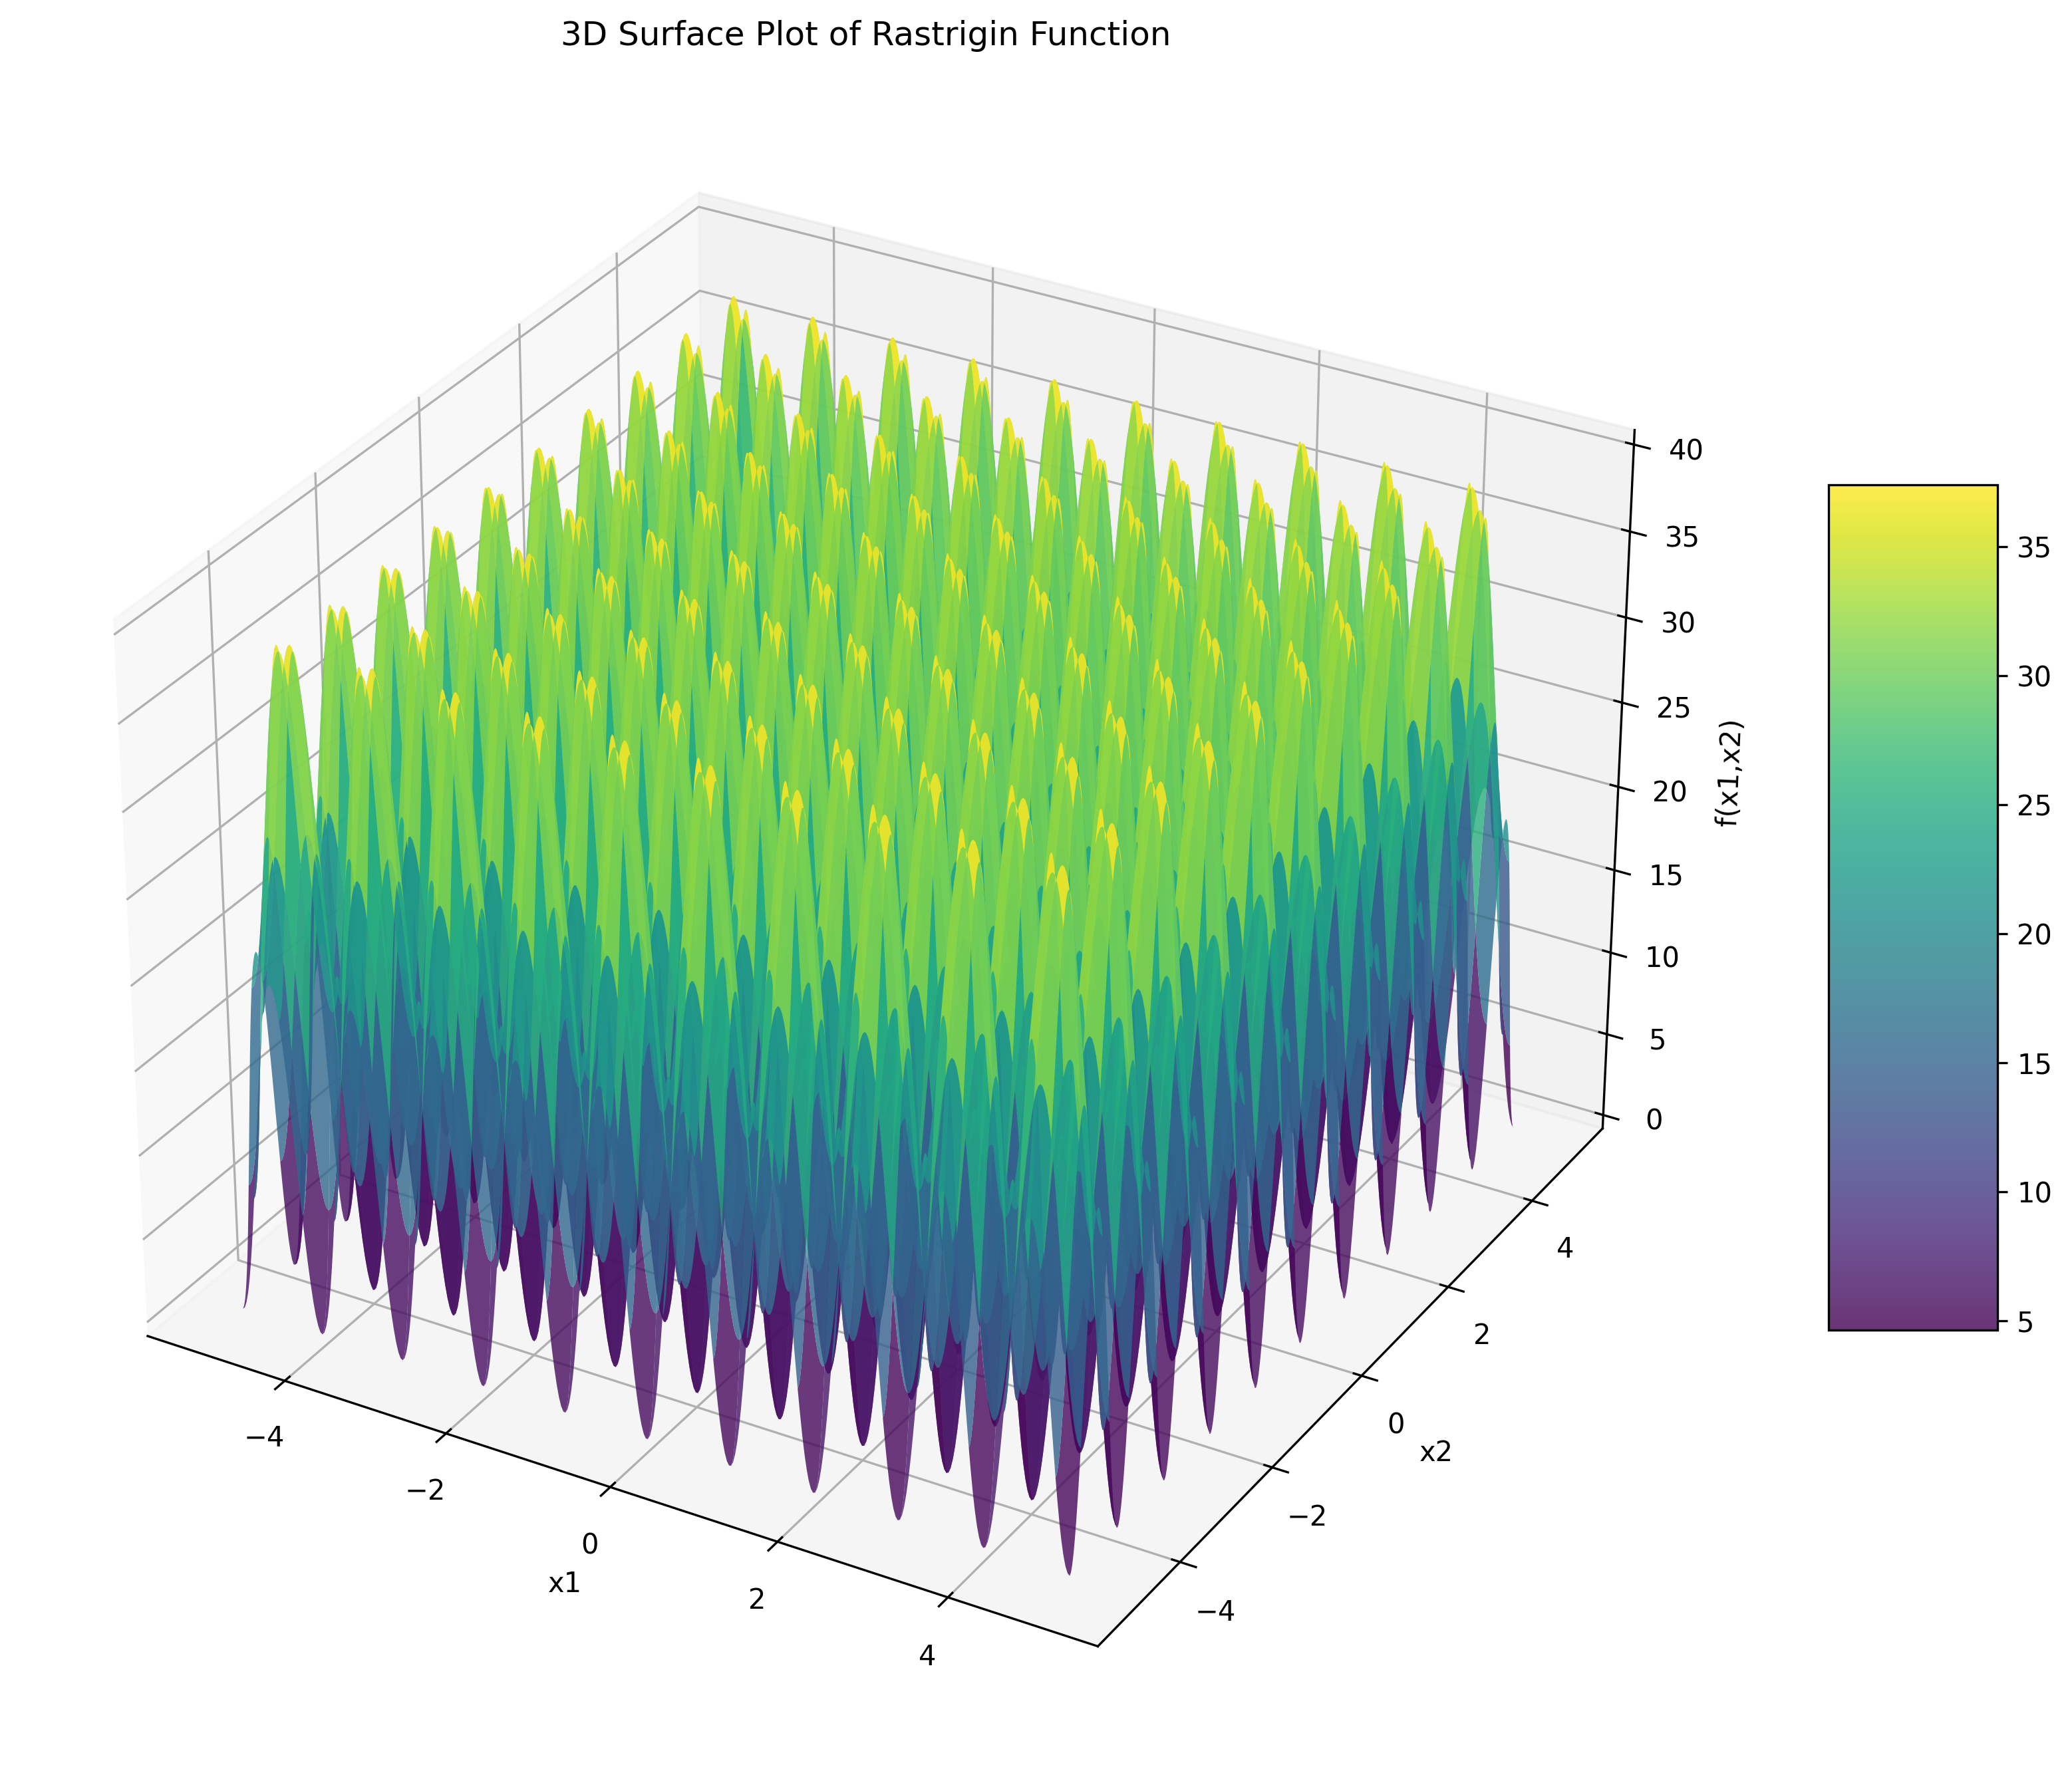
\includegraphics[width=\linewidth]{cec/rastrigin_3d.png}
		\caption{Dimensi 3}
		\label{fig:rastrigin-3d}
	\end{subfigure}
	\caption{Tampilan grafik fungsi Rastrigin pada dimensi dua (\cref{fig:rastrigin-2d}) dan tiga (\cref{fig:rastrigin-3d})}
	\label{fig:rastrigin}
\end{figure}
\begin{flalign*}
  f_{\text{Rastrigin}}(\mathrm{x})=\sum_{i=1}^{D}\left(z_i^2-10\cos\left(2\pi z_i \right)+10\right) +f_{\text{bias}}&&
\end{flalign*}

\subsubsection{Rosenbrock}
\noindent Properti:
\begin{packed_item}
  \item multimodal
  \item non-convex
  \item non-separable
  \item Local optima's number is huge
\end{packed_item}
\begin{figure}[H]
	\centering
	\begin{subfigure}[b]{0.4\textwidth}
		\centering
		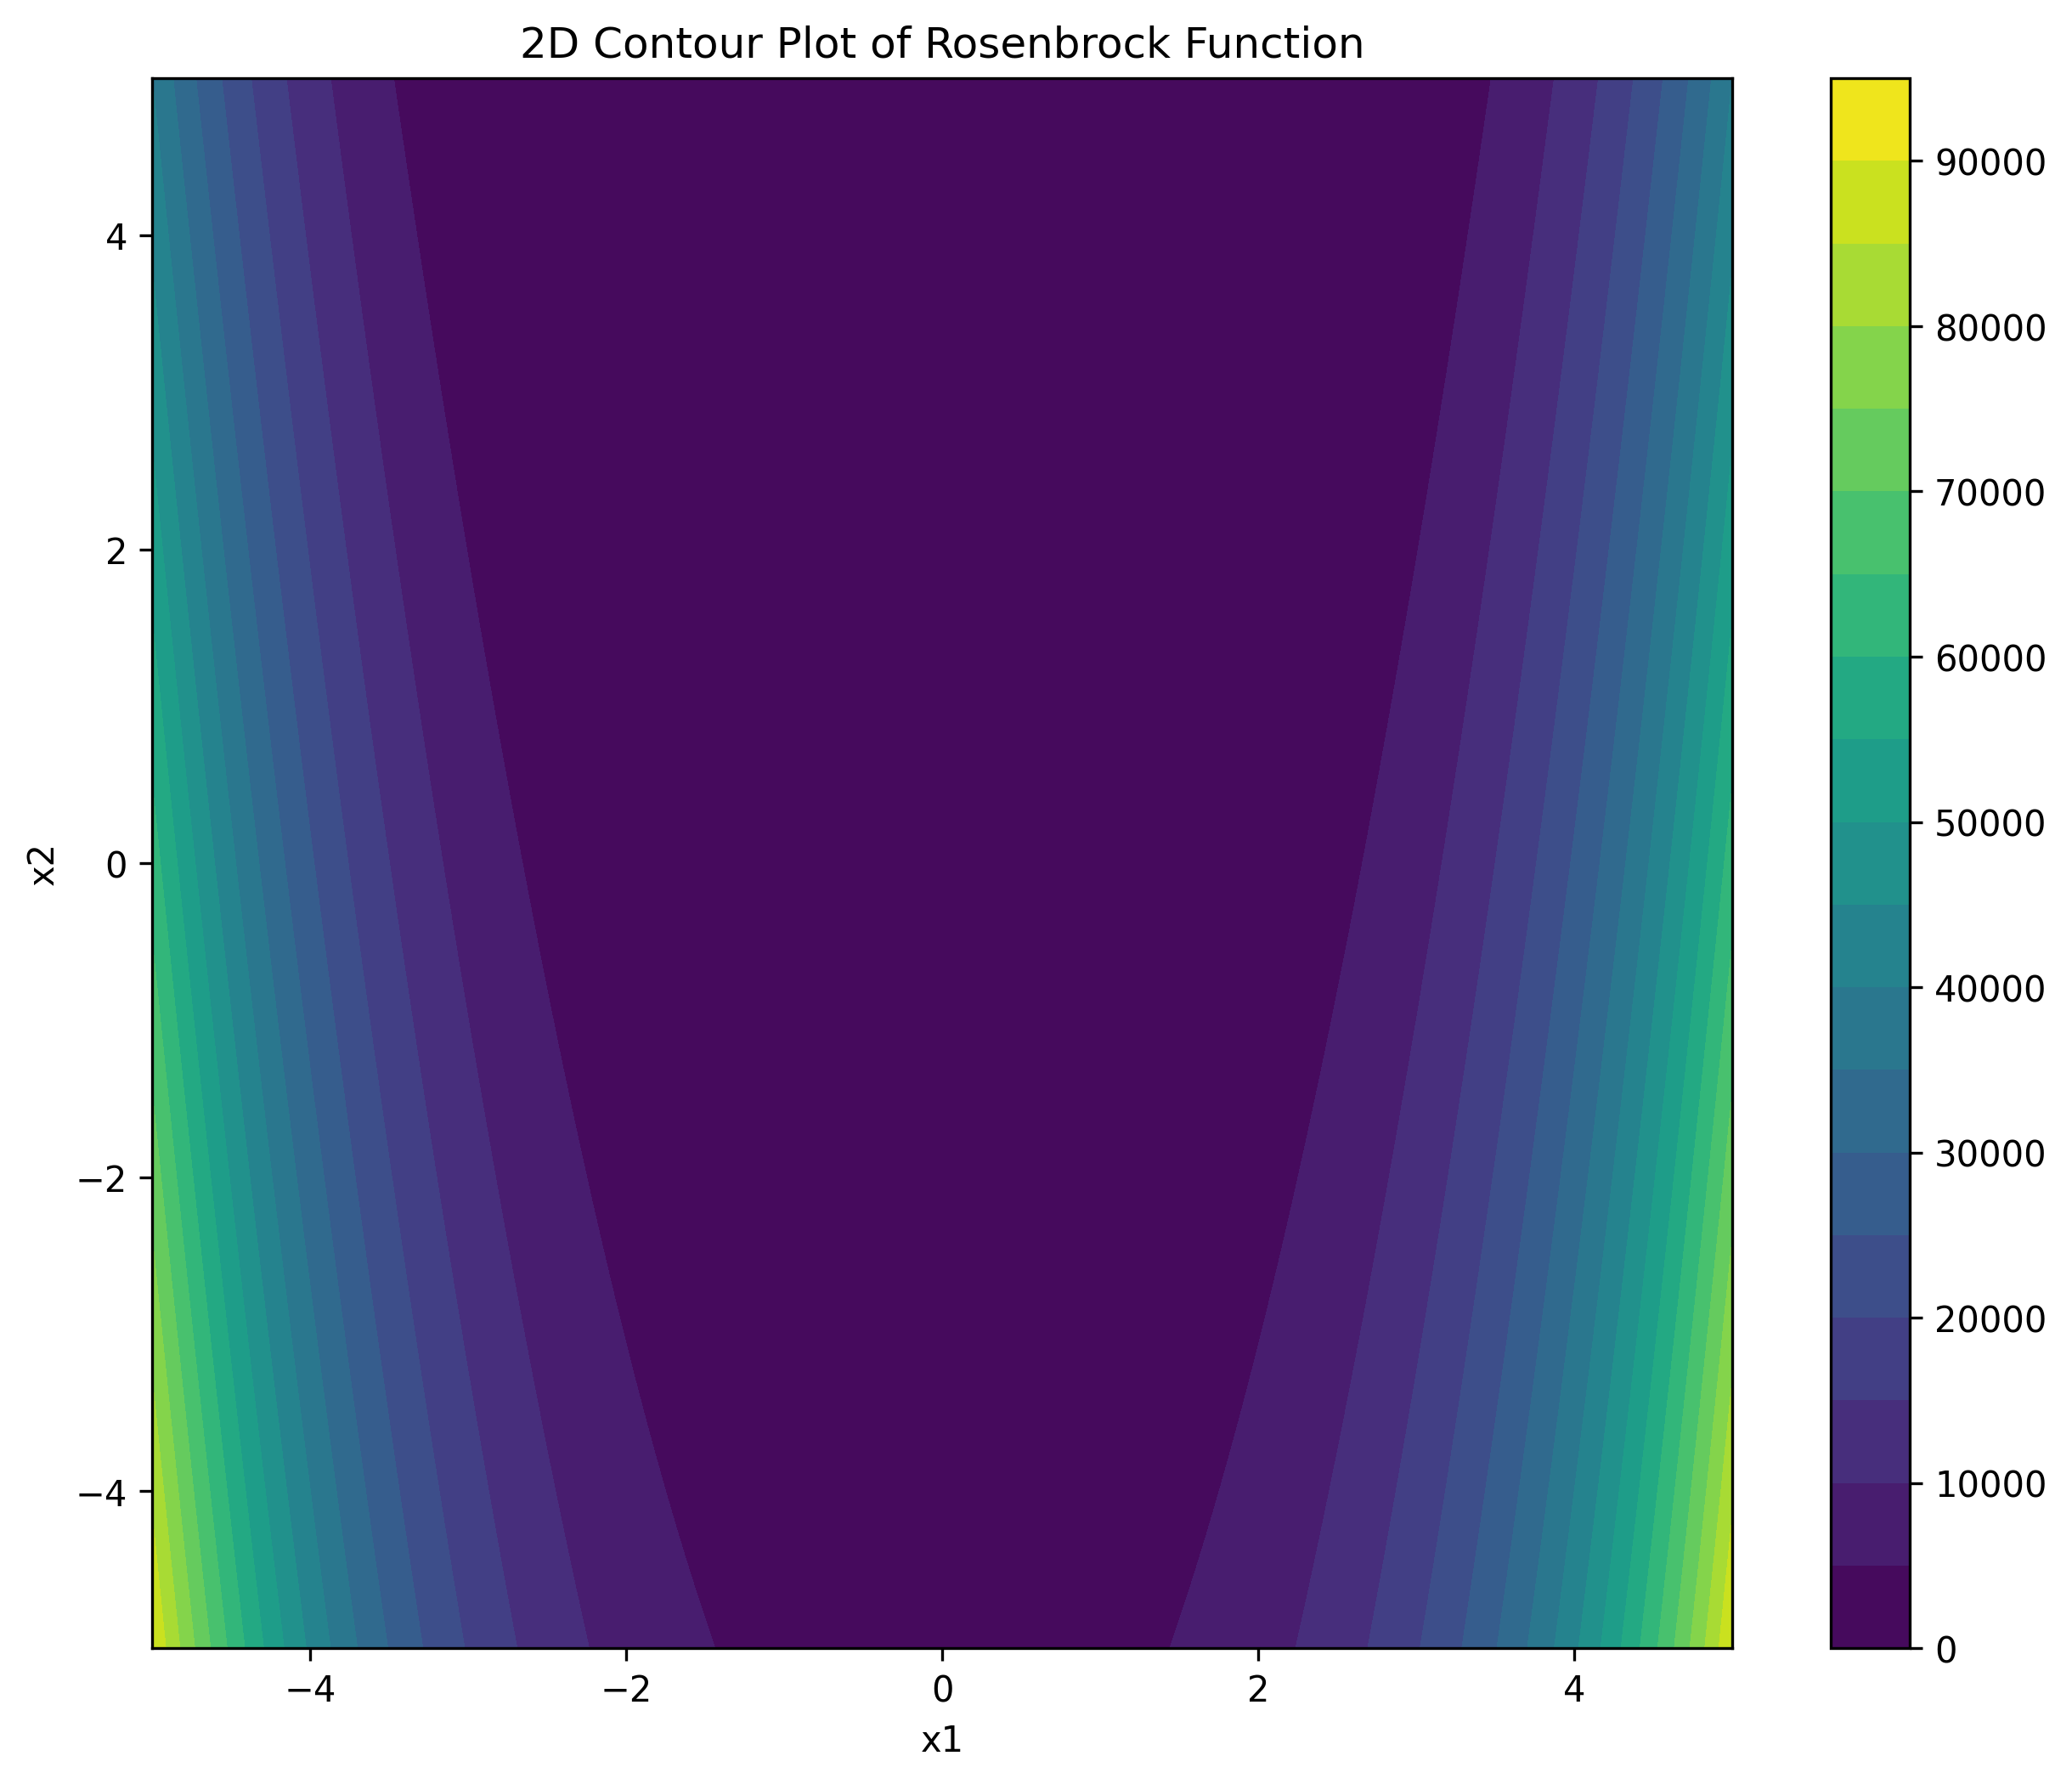
\includegraphics[width=\linewidth]{cec/rosenbrock_2d.png}
		\caption{Dimensi 2}
		\label{fig:rosenbrock-2d}
	\end{subfigure}
	\hfill
	\begin{subfigure}[b]{0.4\textwidth}
		\centering
		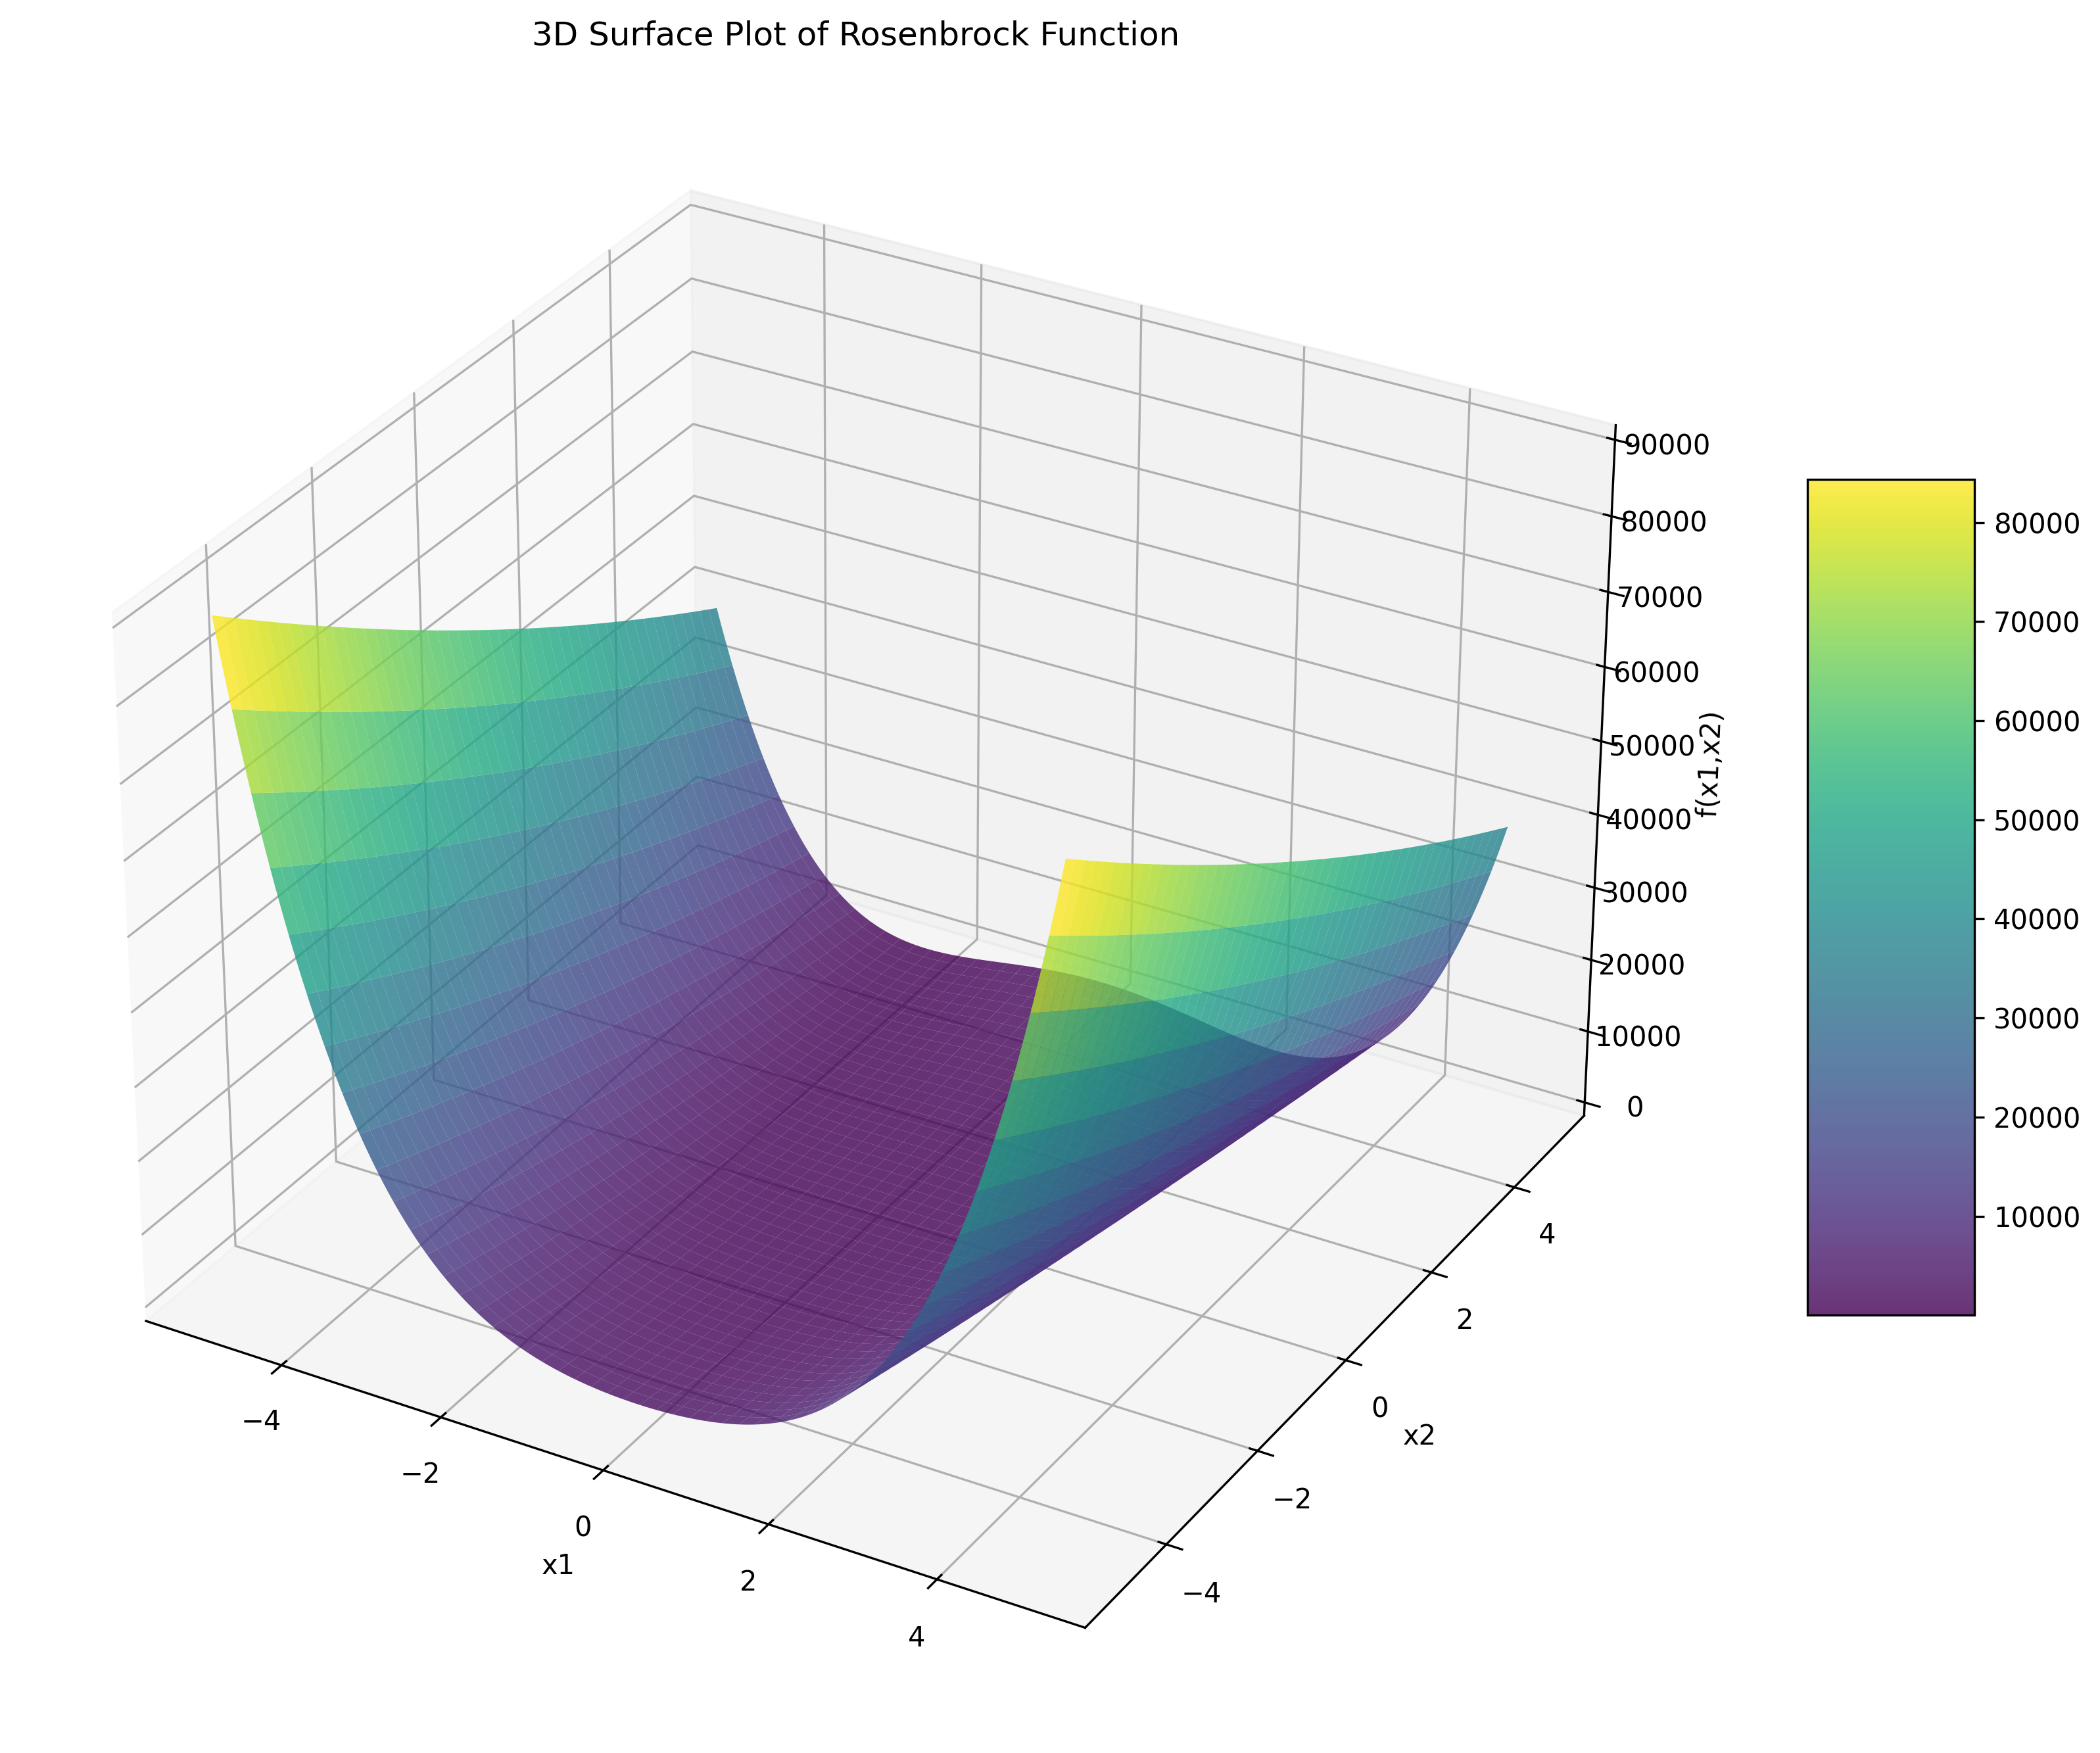
\includegraphics[width=\linewidth]{cec/rosenbrock_3d.png}
		\caption{Dimensi 3}
		\label{fig:rosenbrock-3d}
	\end{subfigure}
	\caption{Tampilan grafik fungsi Rosenbrock pada dimensi dua (\cref{fig:rosenbrock-2d}) dan tiga (\cref{fig:rosenbrock-3d})}
	\label{fig:rosenbrock}
\end{figure}
\begin{flalign*}
  f_{\text{Rosenbrock}}(\mathrm{x})=\sum_{i=1}^{D-1}\left(100\left(z_i^2-z_{i+1} \right)^2+\left( z_i-1\right)^2 \right) +f_{\text{bias}}&&
\end{flalign*}

\subsubsection{Schwefel 1.2 Problem}
\noindent Properti:
\begin{packed_item}
  \item unimodal
  \item convex
  \item non-separable
  \item scalable
\end{packed_item}
\begin{figure}[H]
	\centering
	\begin{subfigure}[b]{0.4\textwidth}
		\centering
		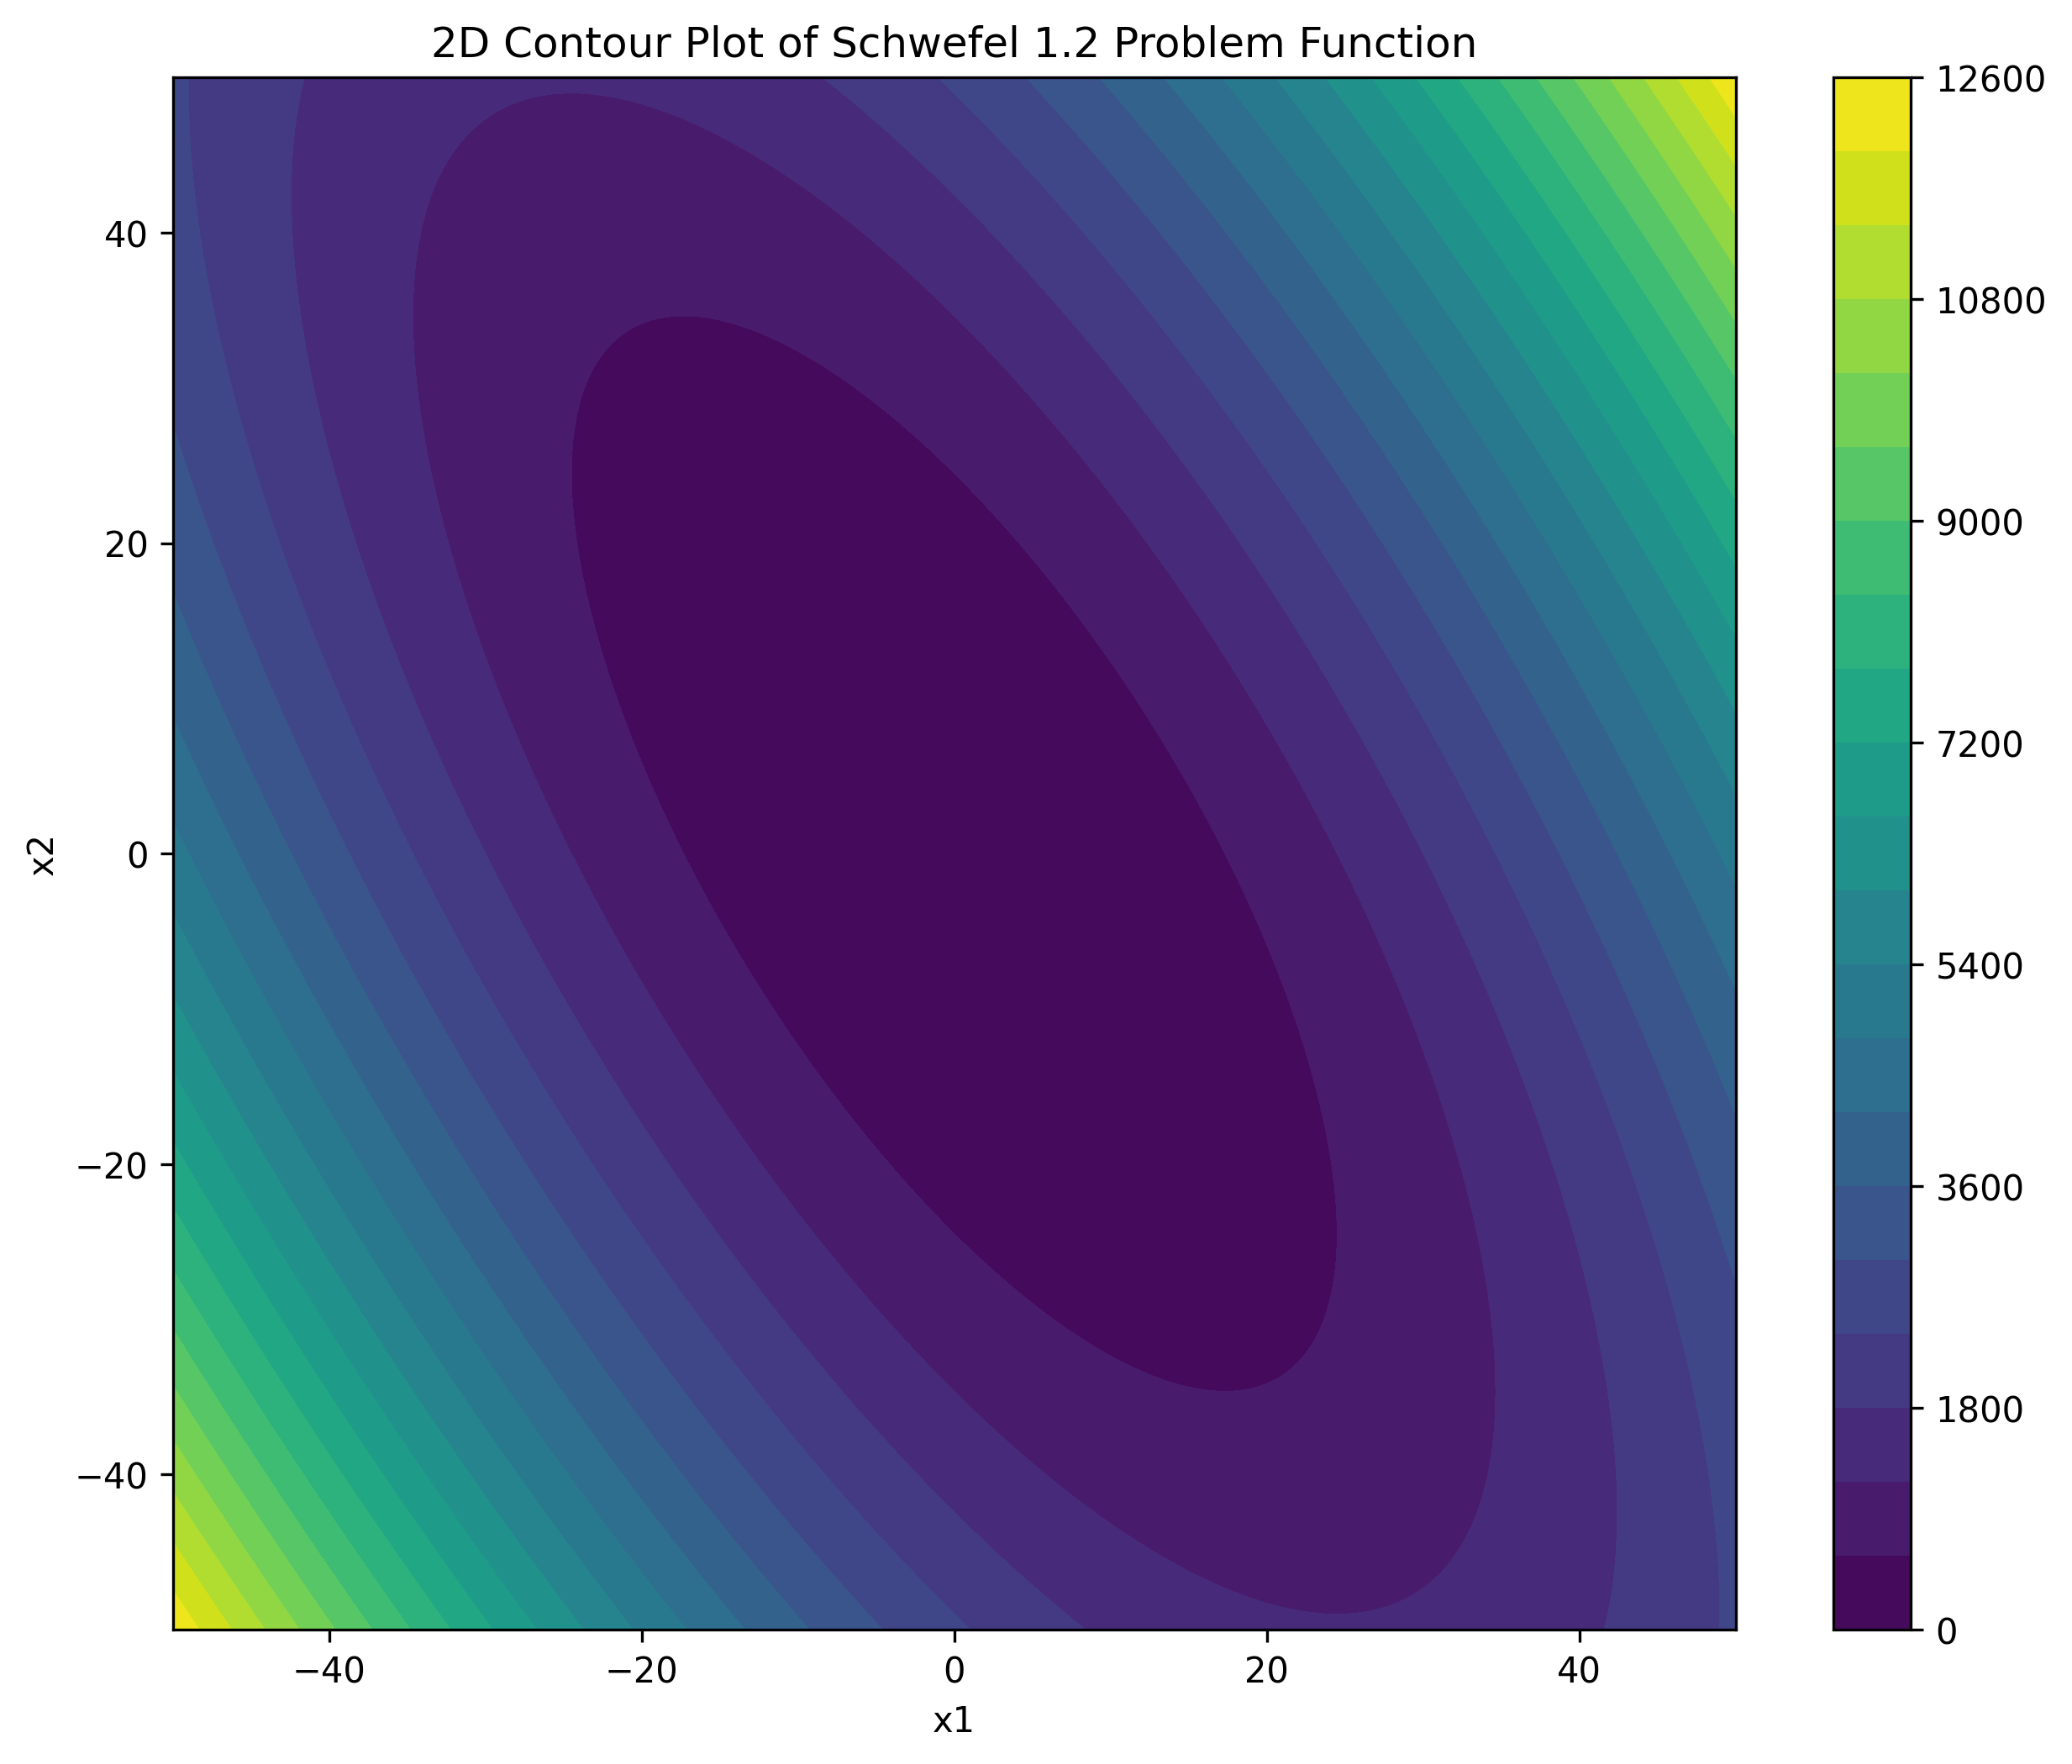
\includegraphics[width=\linewidth]{cec/schwefel1_2_2d.png}
		\caption{Dimensi 2}
		\label{fig:schwefel1_2-2d}
	\end{subfigure}
	\hfill
	\begin{subfigure}[b]{0.4\textwidth}
		\centering
		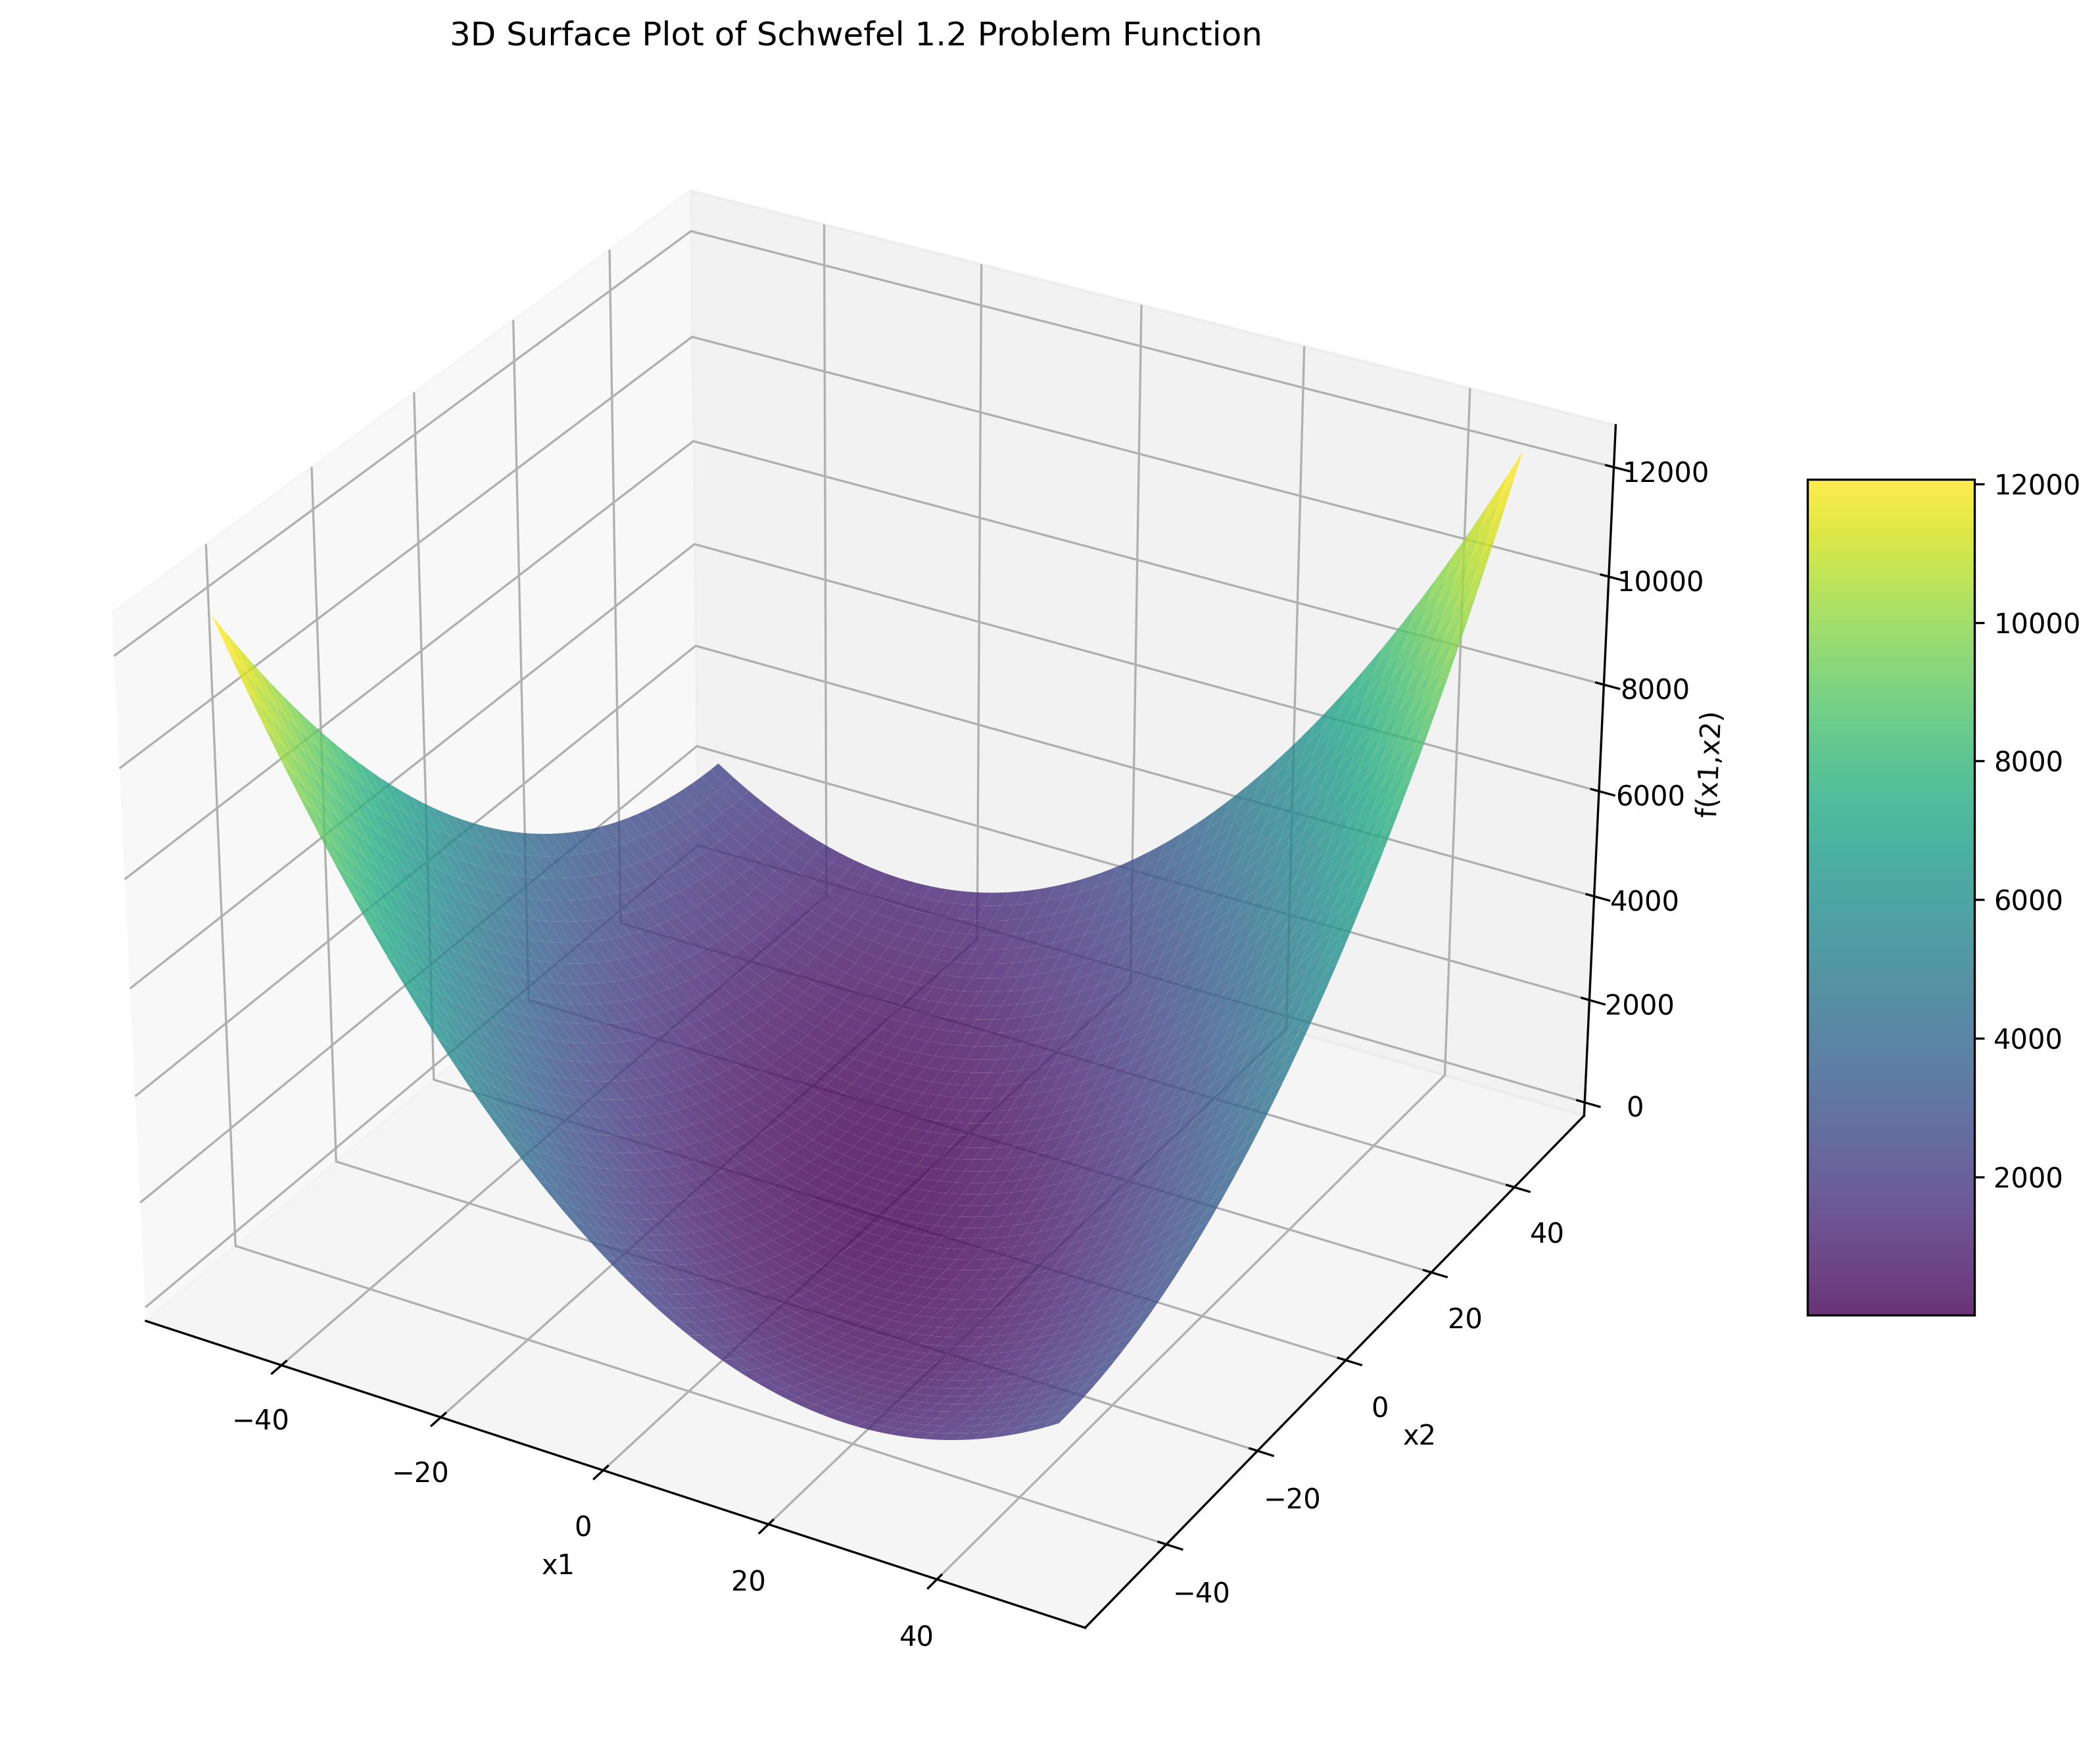
\includegraphics[width=\linewidth]{cec/schwefel1_2_3d.png}
		\caption{Dimensi 3}
		\label{fig:schwefel1_2-3d}
	\end{subfigure}
	\caption{Tampilan grafik fungsi Schwefel 1.2 Problem pada dimensi dua (\cref{fig:schwefel1_2-2d}) dan tiga (\cref{fig:schwefel1_2-3d})}
	\label{fig:schwefel1_2}
\end{figure}
\begin{flalign*}
  f_{\text{Schwefel 1.2}}(\mathrm{x})=\sum_{i=1}^{D}\left(\sum_{j=1}^{i}z_j \right)^2 +f_{\text{bias}}&&
\end{flalign*}

\subsubsection{Schwefel 2.13 Problem}
\noindent Properti:
\begin{packed_item}
  \item multimodal
  \item non-convex
  \item non-separable
  \item scalable
\end{packed_item}
\begin{figure}[H]
	\centering
	\begin{subfigure}[b]{0.4\textwidth}
		\centering
		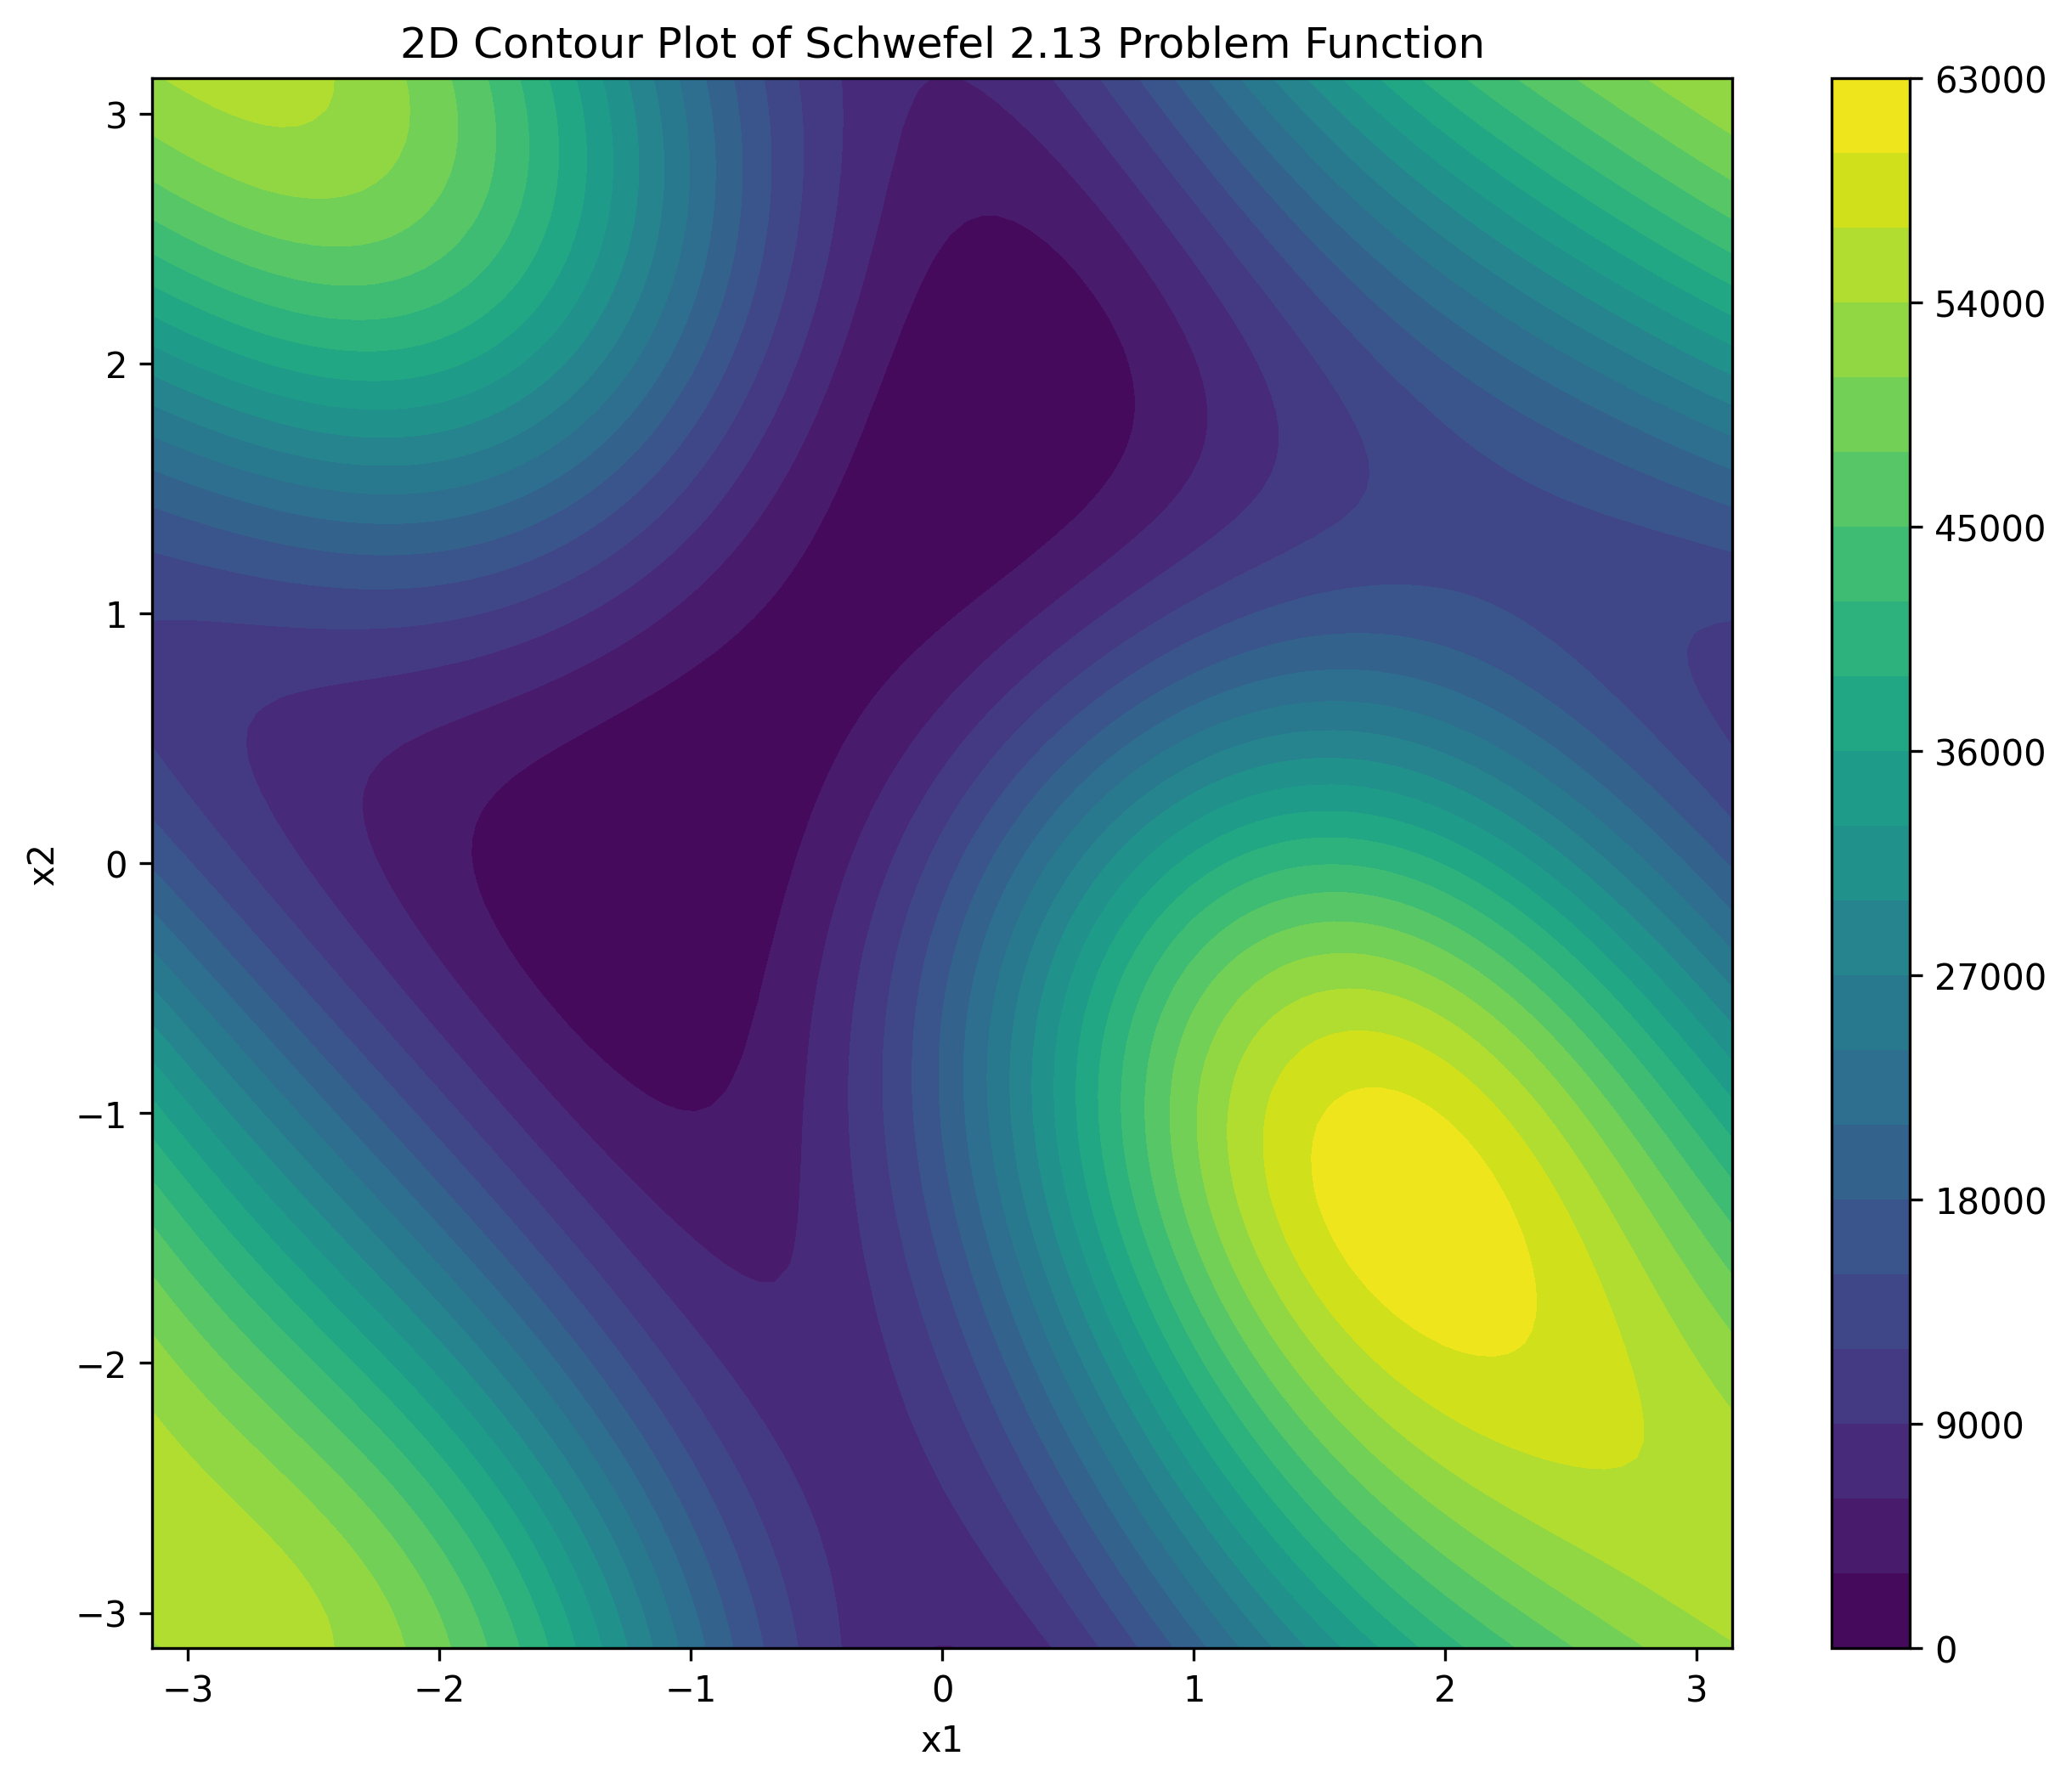
\includegraphics[width=\linewidth]{cec/schwefel2_13_2d.png}
		\caption{Dimensi 2}
		\label{fig:schwefel2_13-2d}
	\end{subfigure}
	\hfill
	\begin{subfigure}[b]{0.4\textwidth}
		\centering
		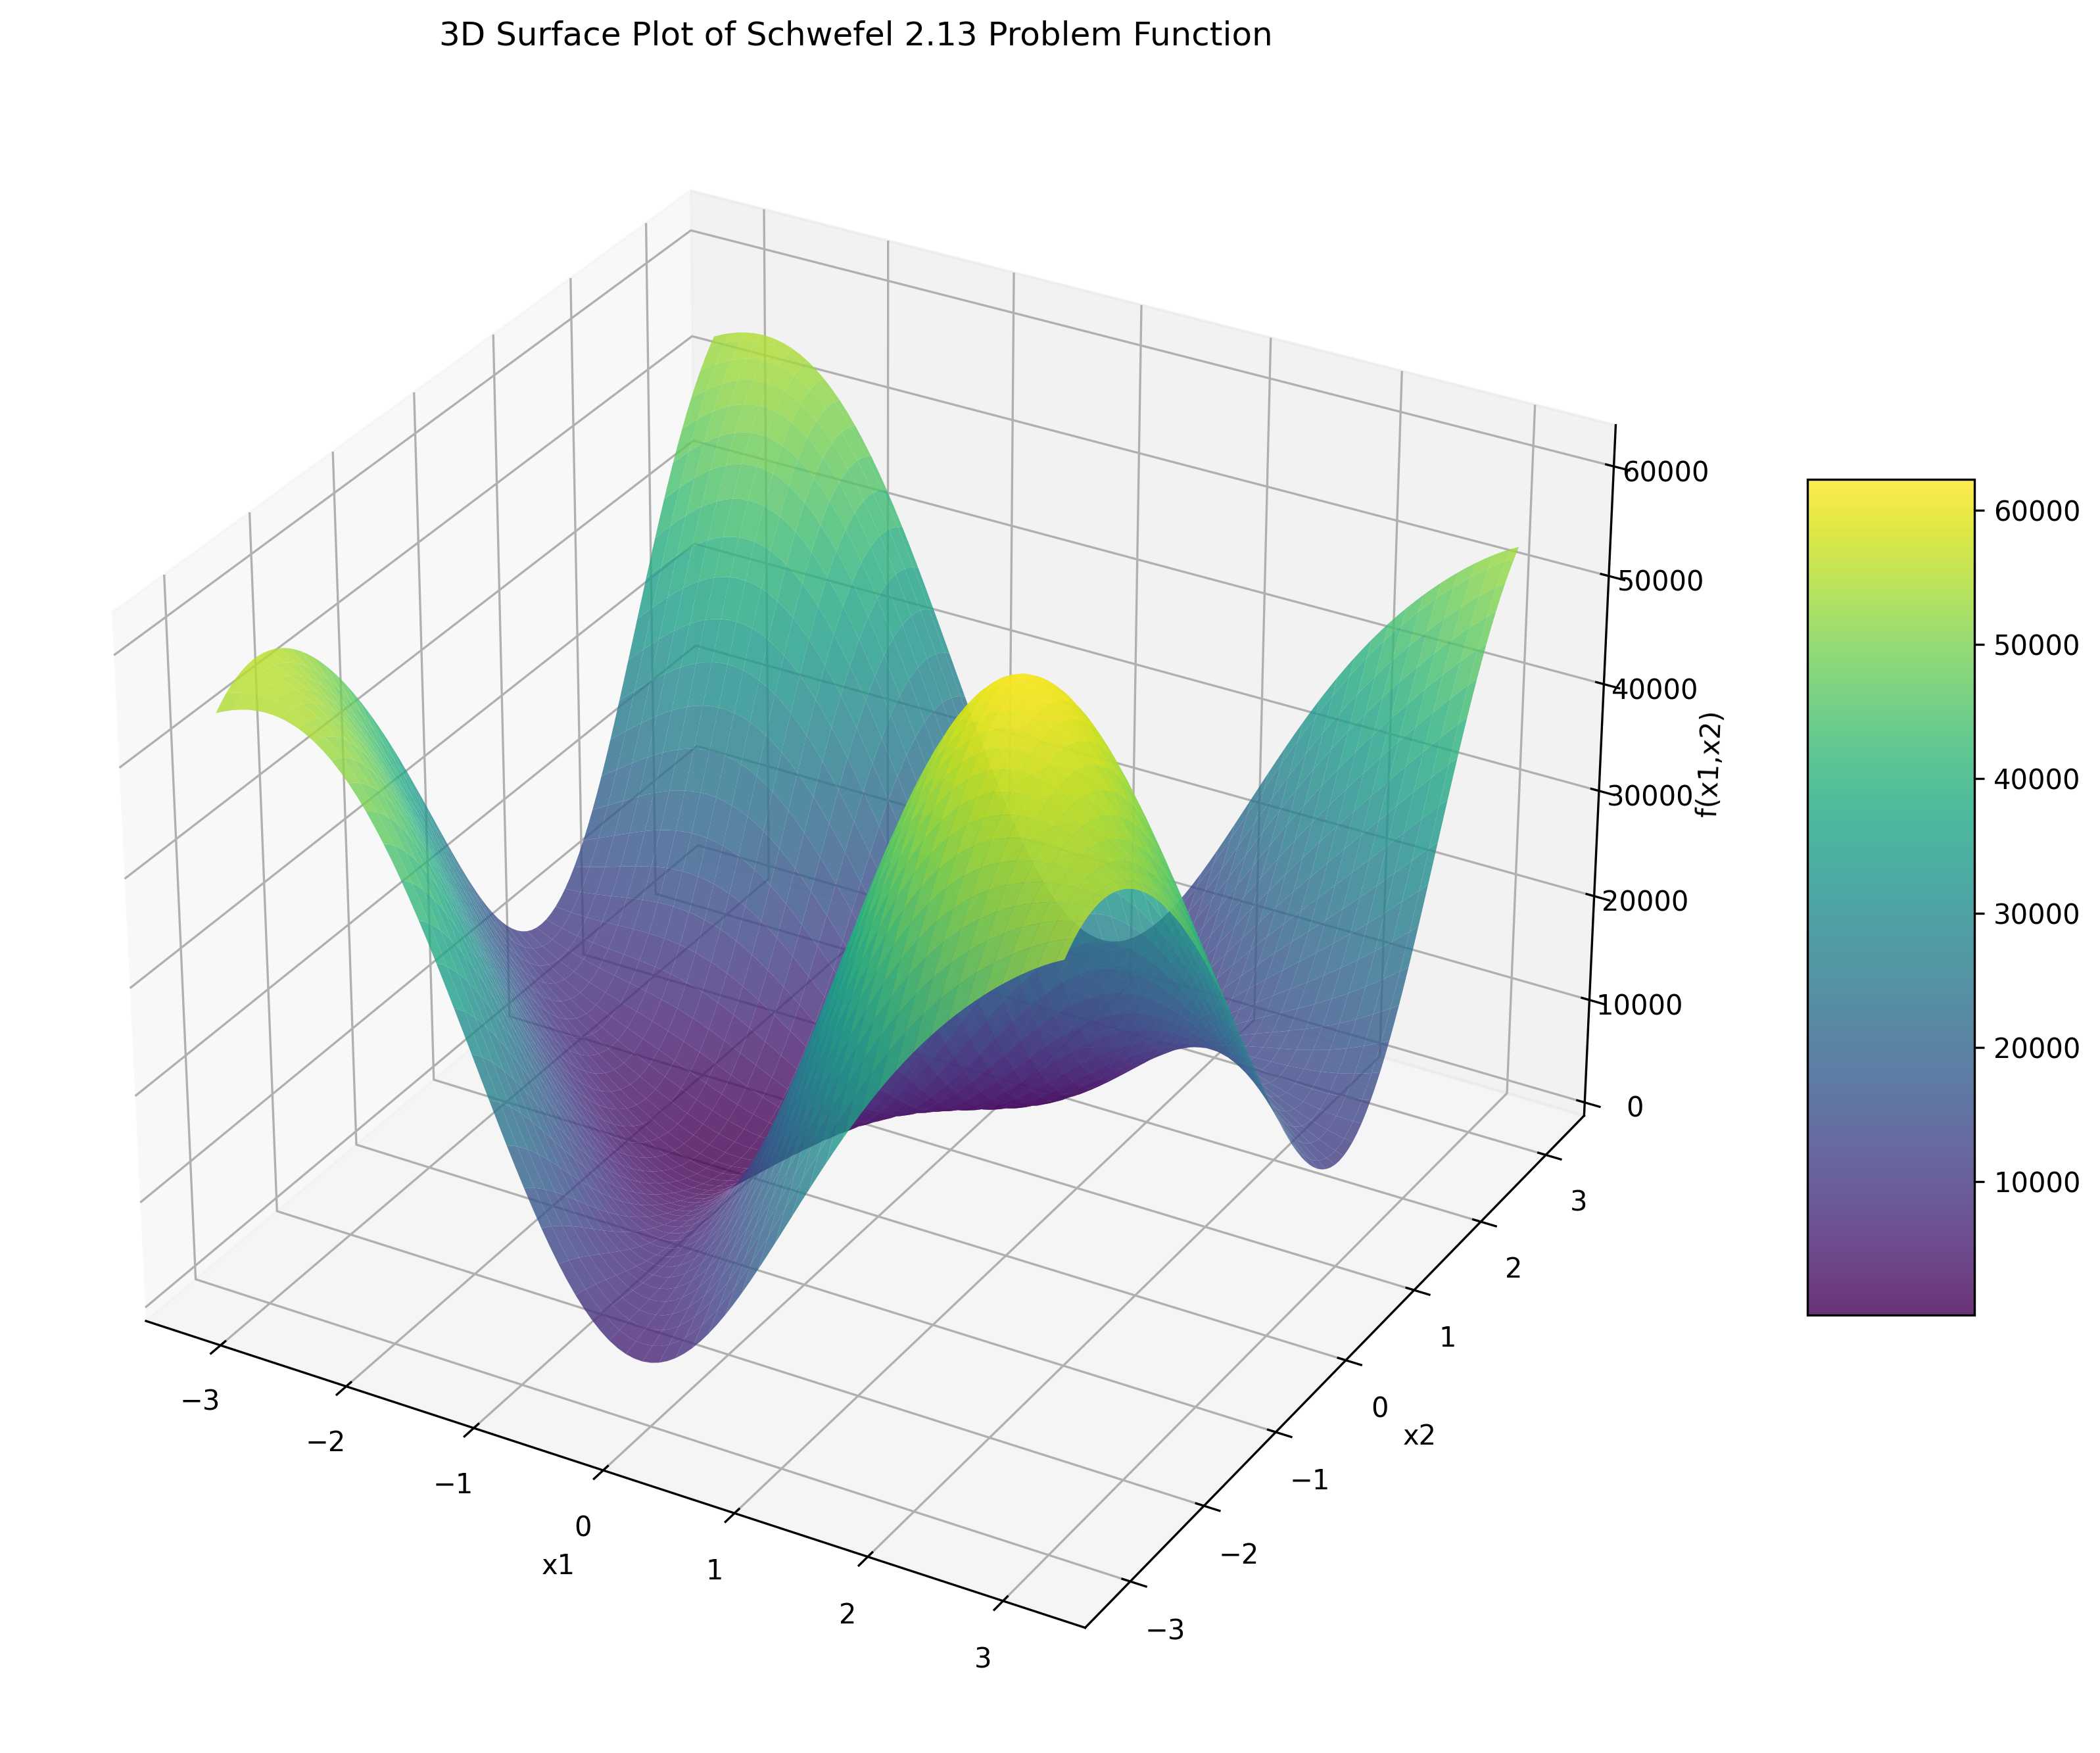
\includegraphics[width=\linewidth]{cec/schwefel2_13_3d.png}
		\caption{Dimensi 3}
		\label{fig:schwefel2_13-3d}
	\end{subfigure}
	\caption{Tampilan grafik fungsi Schwefel 2.13 Problem pada dimensi dua (\cref{fig:schwefel2_13-2d}) dan tiga (\cref{fig:schwefel2_13-3d})}
	\label{fig:schwefel2_13}
\end{figure}
\begin{flalign*}
  &f_{\text{Schwefel 2.13}}(\mathrm{x})=\sum_{i=1}^{D}\left(\mathrm{A}_i-\mathrm{B}_i\left(z \right)\right)^2 +f_{\text{bias}}&&\\
  &\mathrm{A}_i=\sum_{j=1}^{D}\left(a_{ij}\sin\alpha_j+b_{ij}\cos\alpha_j \right),\mathrm{B}_i\left(z \right)=\sum_{j=1}^{D}\left(a_{ij}\sin z_j+b_{ij}\cos z_j \right), \text{untuk}\ i=1,\ldots,D&&\\
  &\mathrm{A}, \mathrm{B}\text{ adalah dua}\ D*D\ \text{matriks}, a_{ij},b_{ij}\ \text{adalah bilangan bulat acak dalam rentang}\left[-100,100 \right]&&\\
  &\alpha=\left[\alpha_1,\alpha_2,\ldots,\alpha_D \right],\alpha_j\ \text{adalah angka acak dalam rentang}\left[ -\pi,\pi\right]&&
\end{flalign*}

\subsubsection{Shubert}
\noindent Properti:
\begin{packed_item}
  \item multimodal
  \item non-convex
\end{packed_item}
\begin{figure}[H]
	\centering
	\begin{subfigure}[b]{0.4\textwidth}
		\centering
		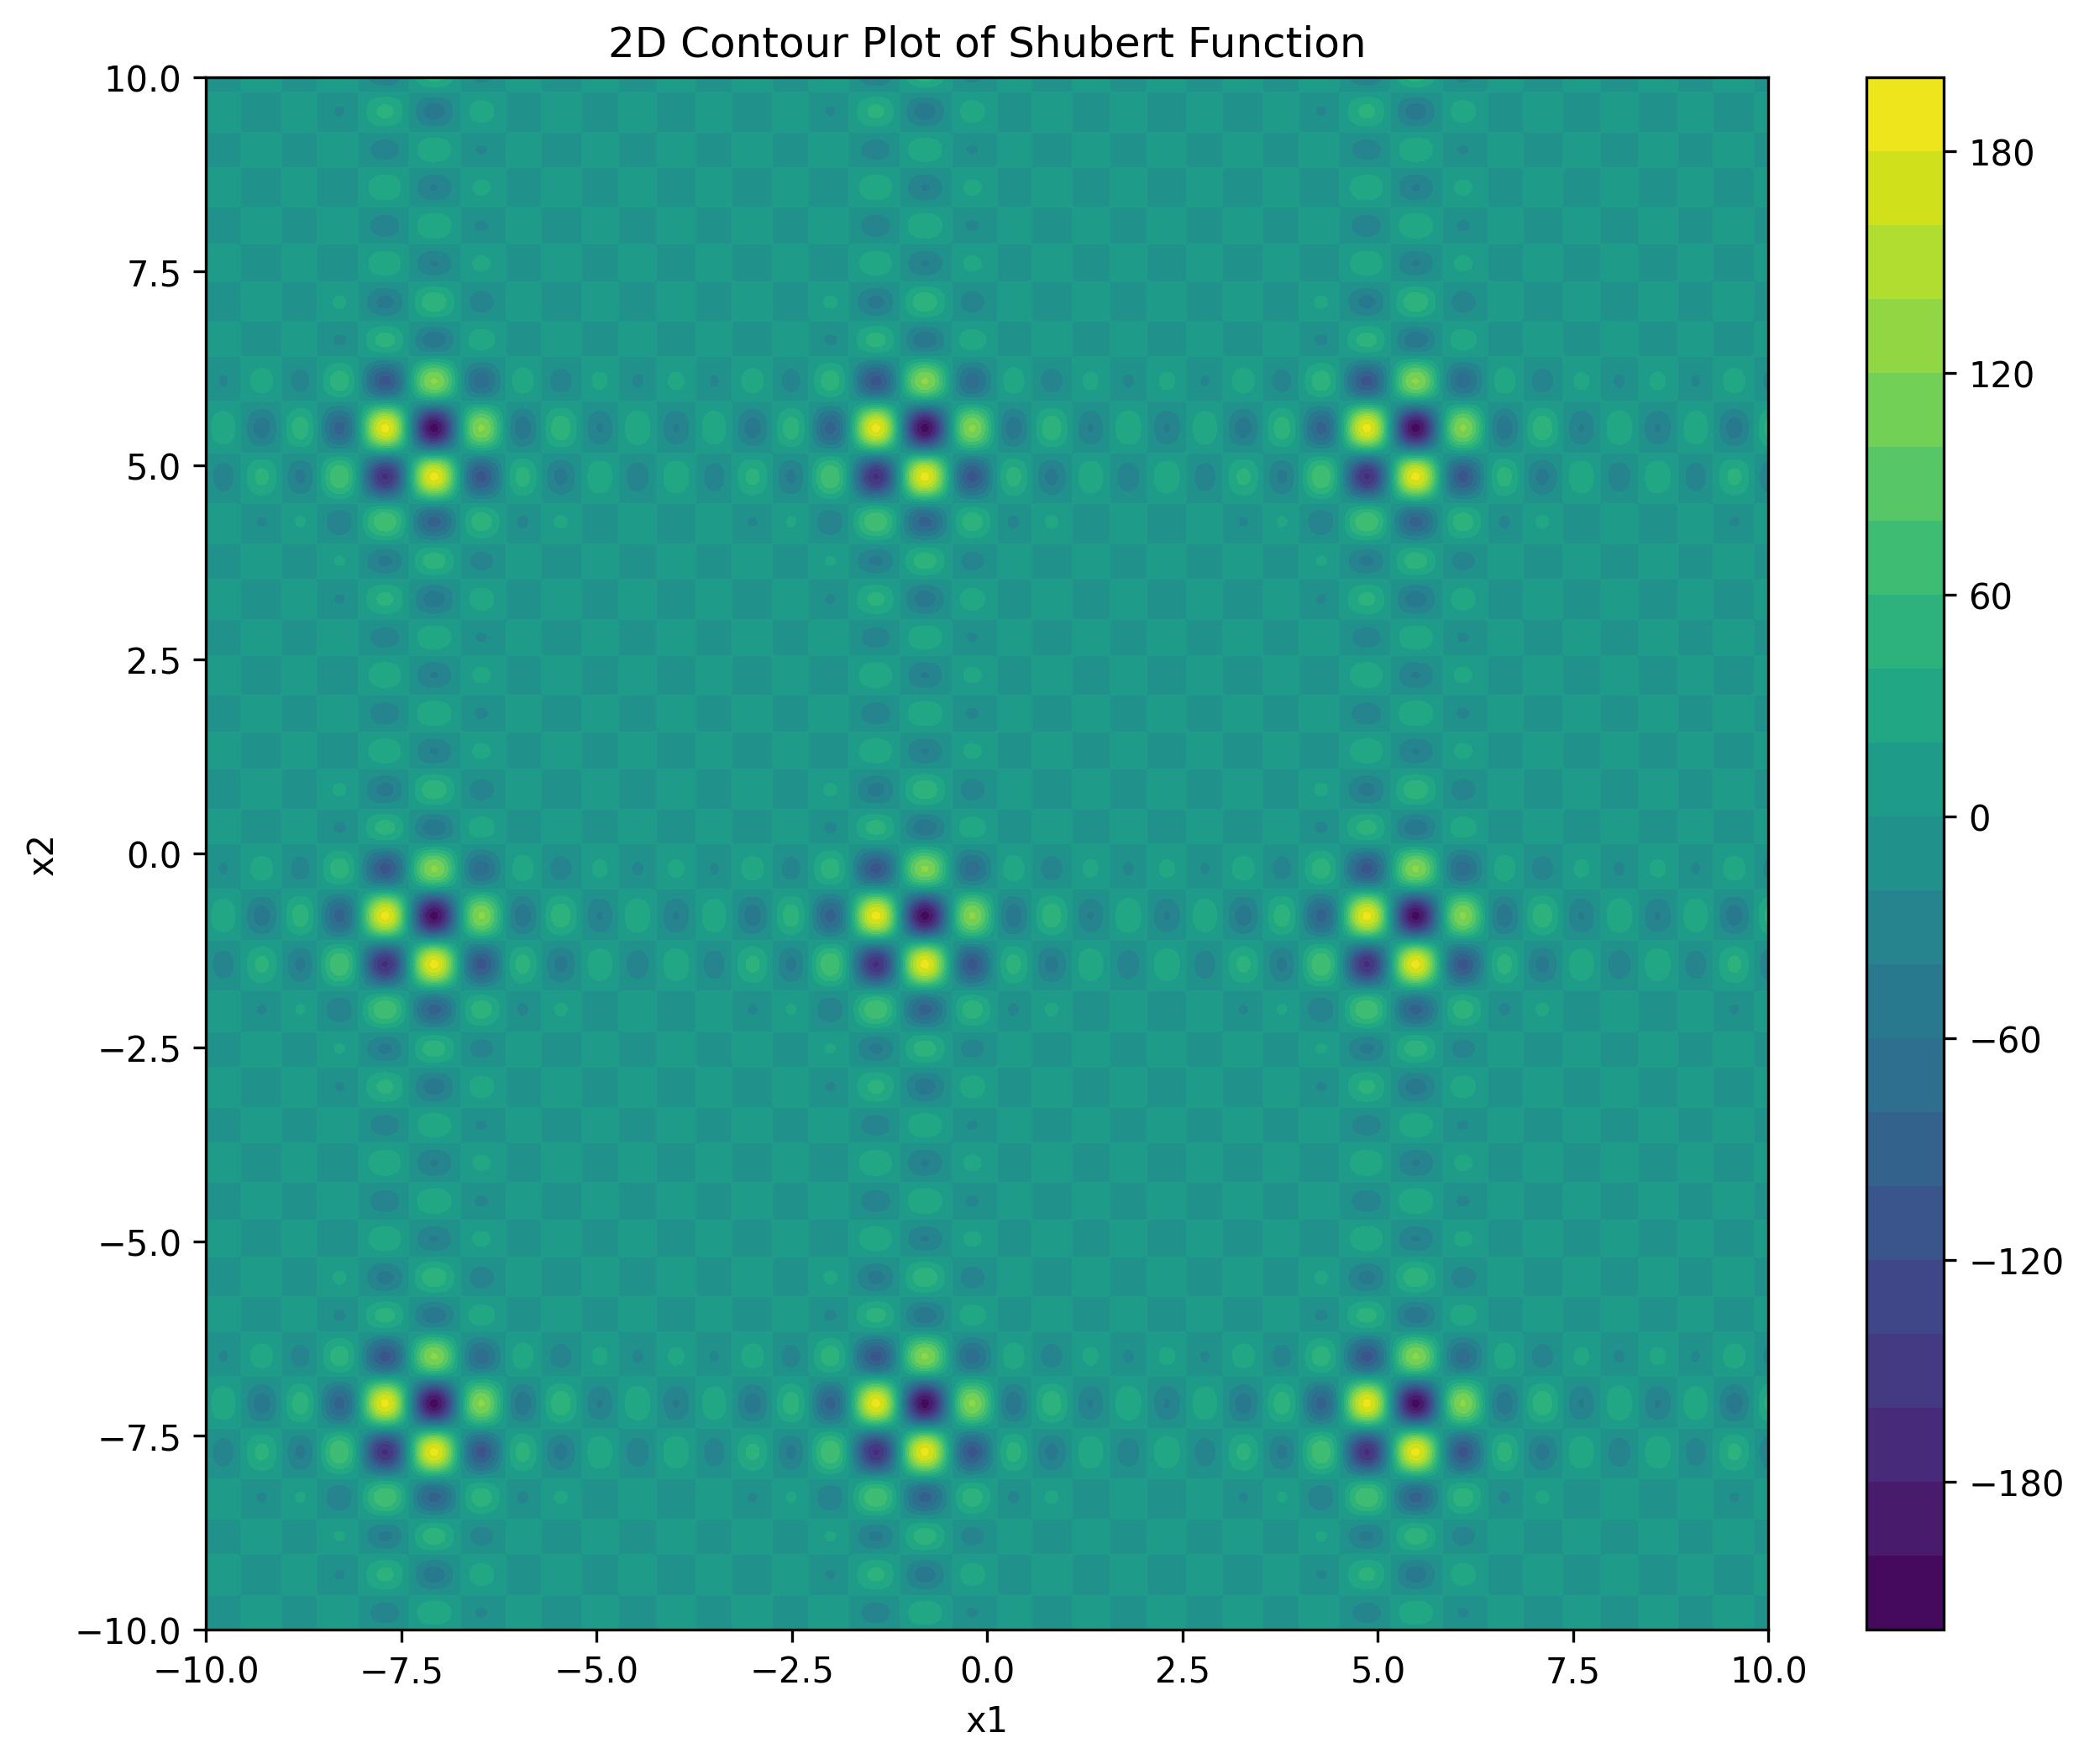
\includegraphics[width=\linewidth]{cec/shubert_2d.png}
		\caption{Dimensi 2}
		\label{fig:shubert-2d}
	\end{subfigure}
	\hfill
	\begin{subfigure}[b]{0.4\textwidth}
		\centering
		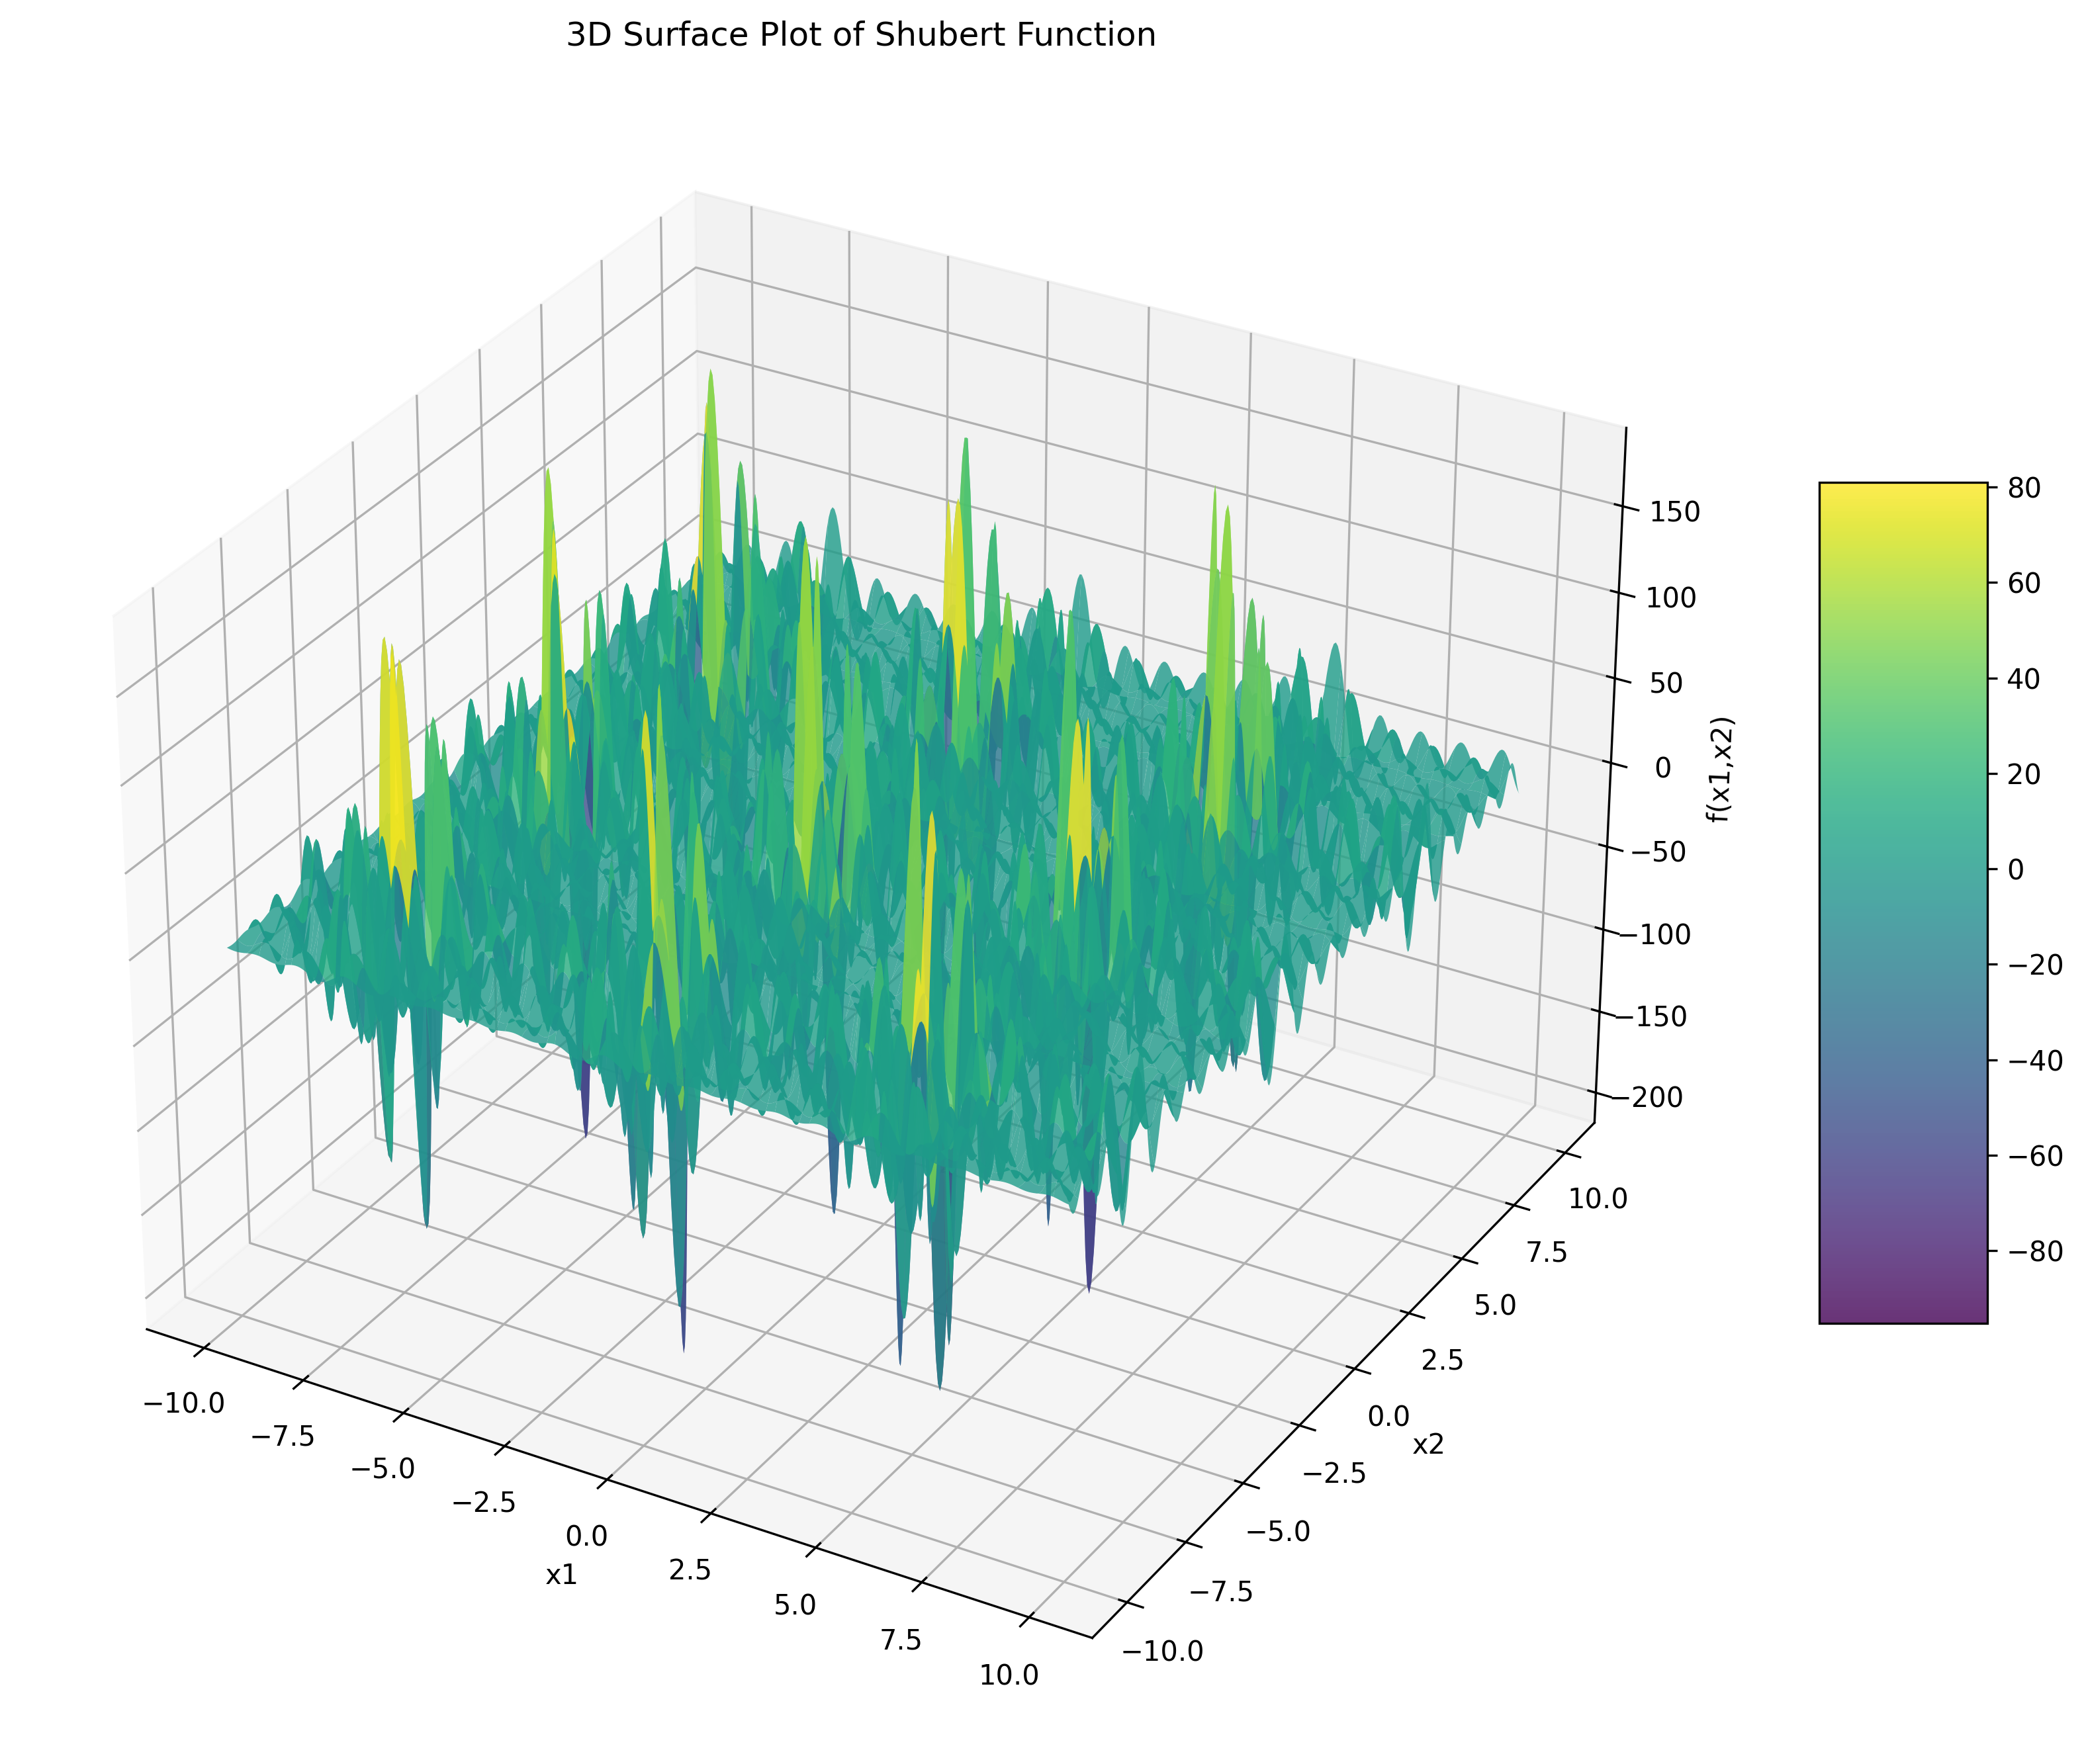
\includegraphics[width=\linewidth]{cec/shubert_3d.png}
		\caption{Dimensi 3}
		\label{fig:shubert-3d}
	\end{subfigure}
	\caption{Tampilan grafik fungsi Shubert pada dimensi dua (\cref{fig:shubert-2d}) dan tiga (\cref{fig:shubert-3d})}
	\label{fig:shubert}
\end{figure}
\begin{flalign*}
  f_{\text{Shubert}}(\mathrm{x})=-\prod_{i=1}^{D}\sum_{j=i}^{5}j\cos\left[\left(j+1 \right)z_i+j  \right]  +f_{\text{bias}}&&
\end{flalign*}

\subsubsection{Sphere}
\noindent Properti:
\begin{packed_item}
  \item unimodal
  \item convex
  \item separable
\end{packed_item}
\begin{figure}[H]
	\centering
	\begin{subfigure}[b]{0.4\textwidth}
		\centering
		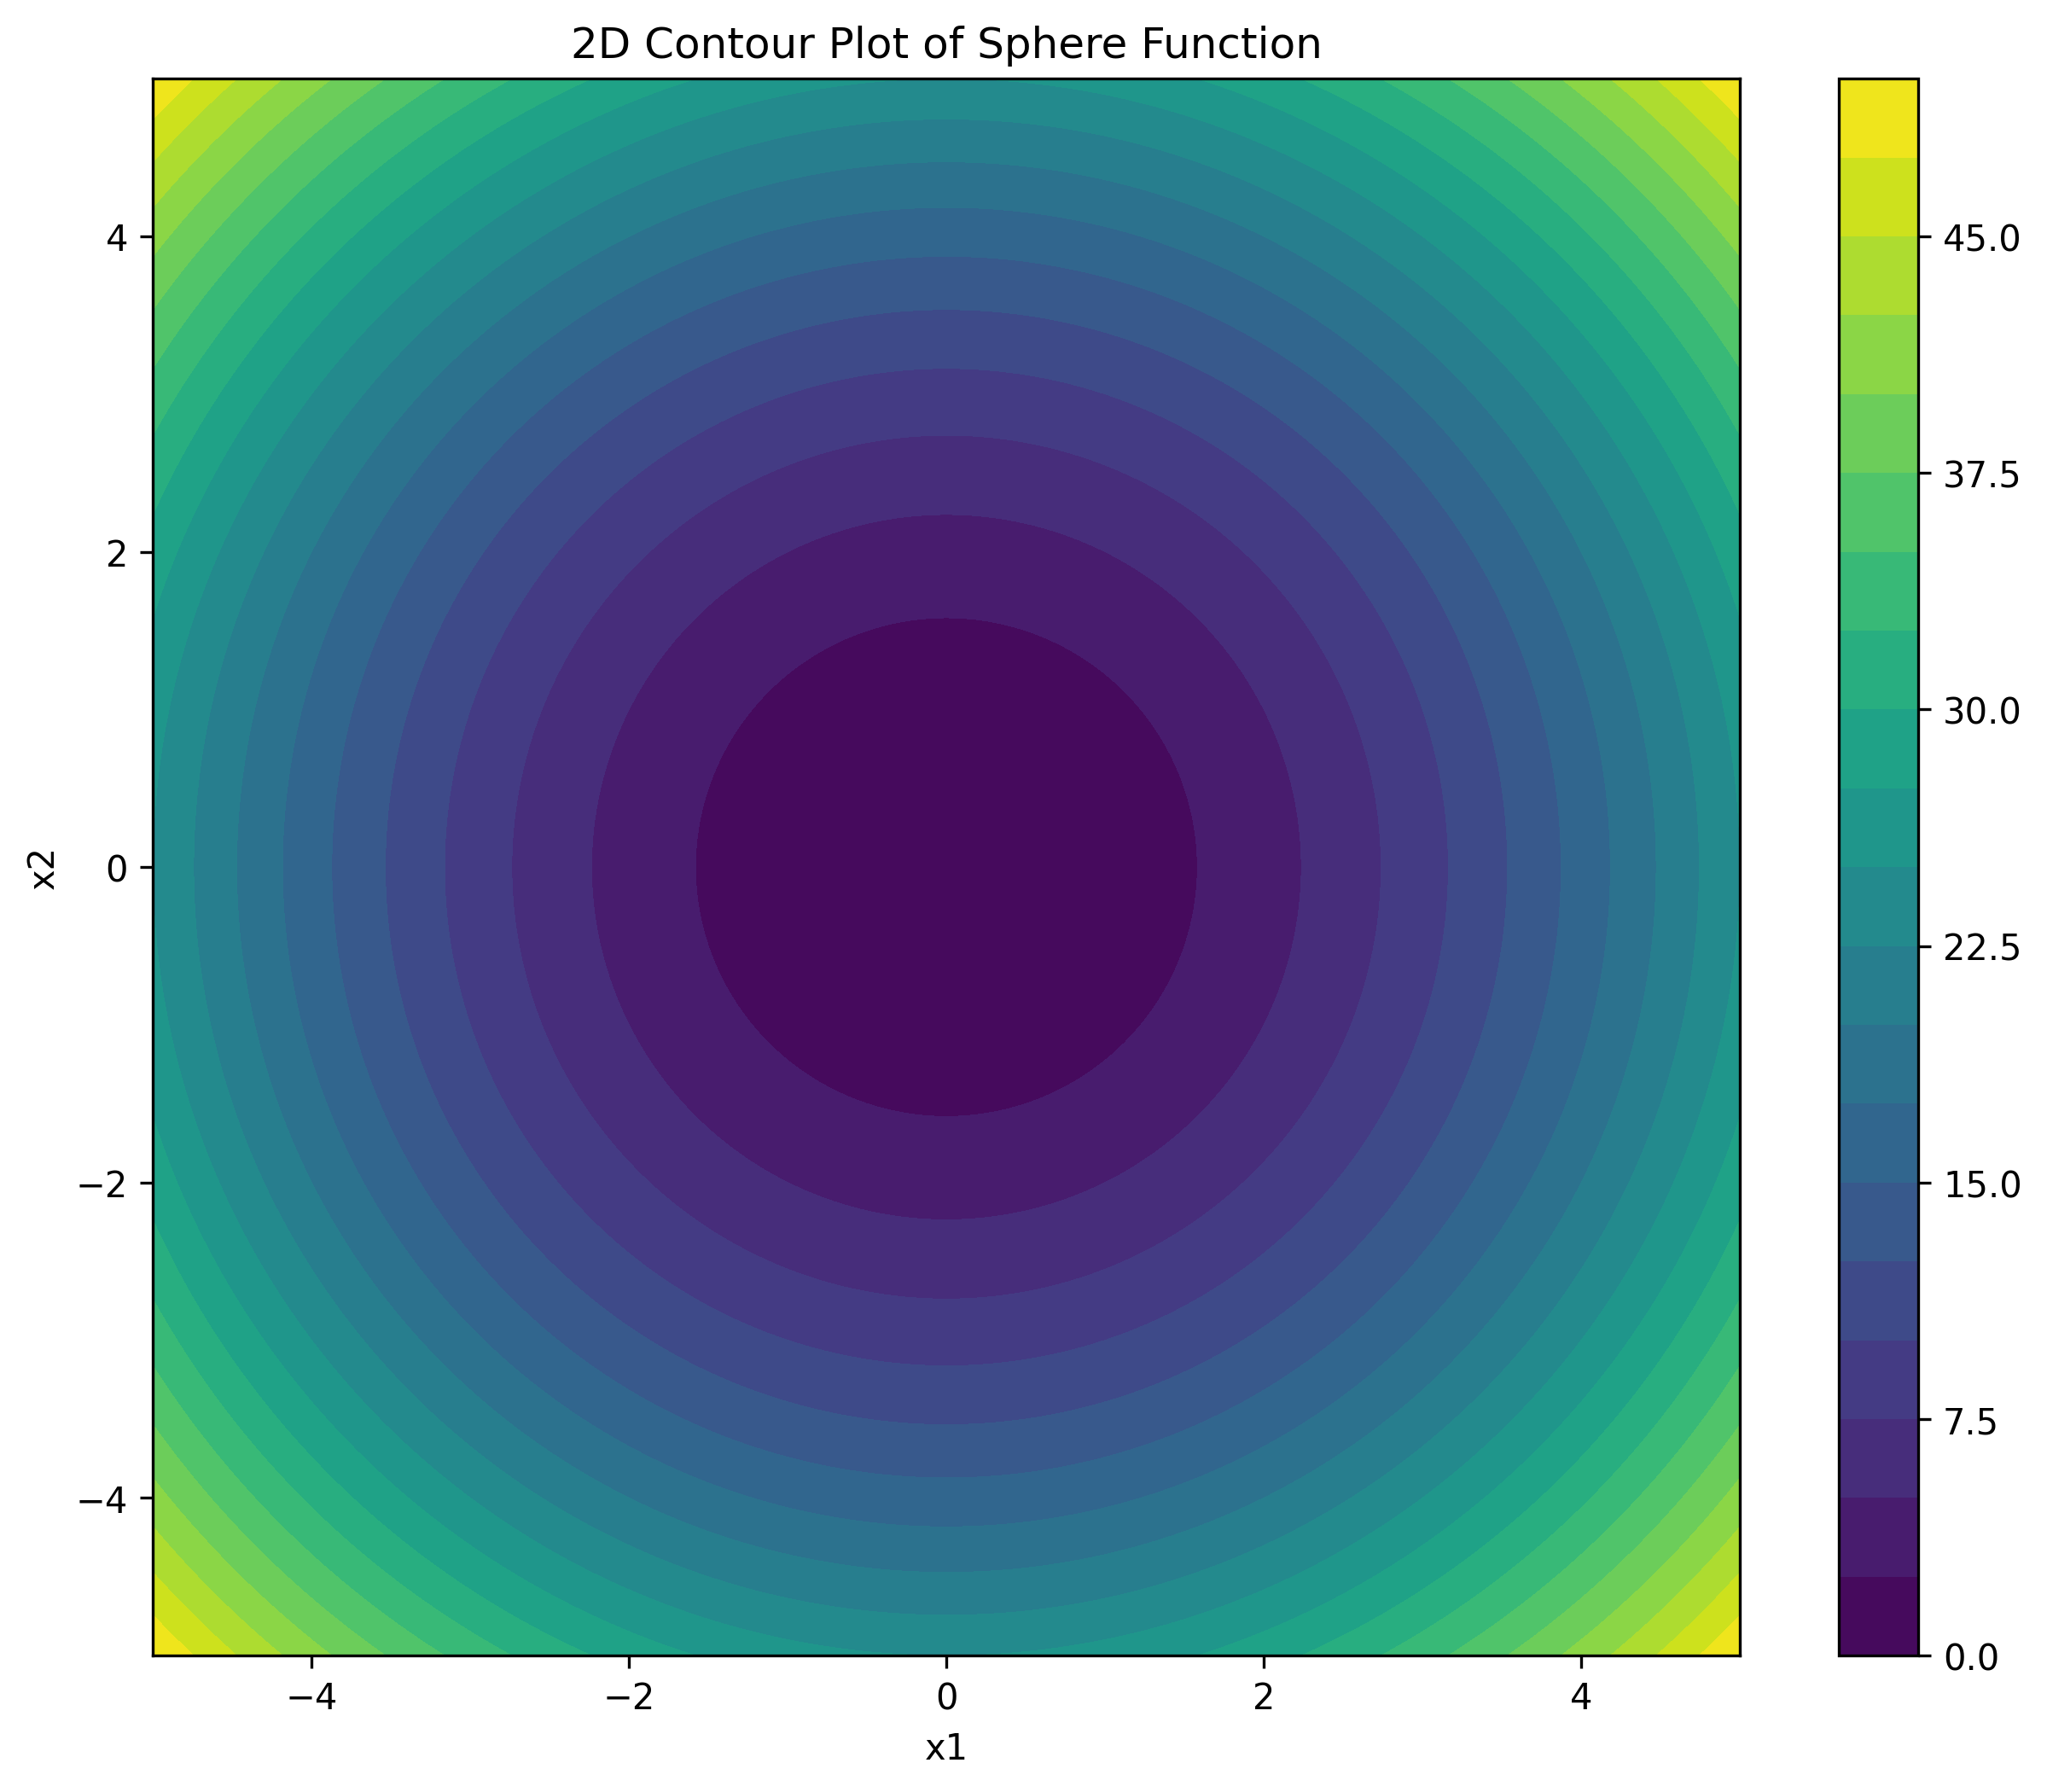
\includegraphics[width=\linewidth]{cec/sphere_2d.png}
		\caption{Dimensi 2}
		\label{fig:sphere-2d}
	\end{subfigure}
	\hfill
	\begin{subfigure}[b]{0.4\textwidth}
		\centering
		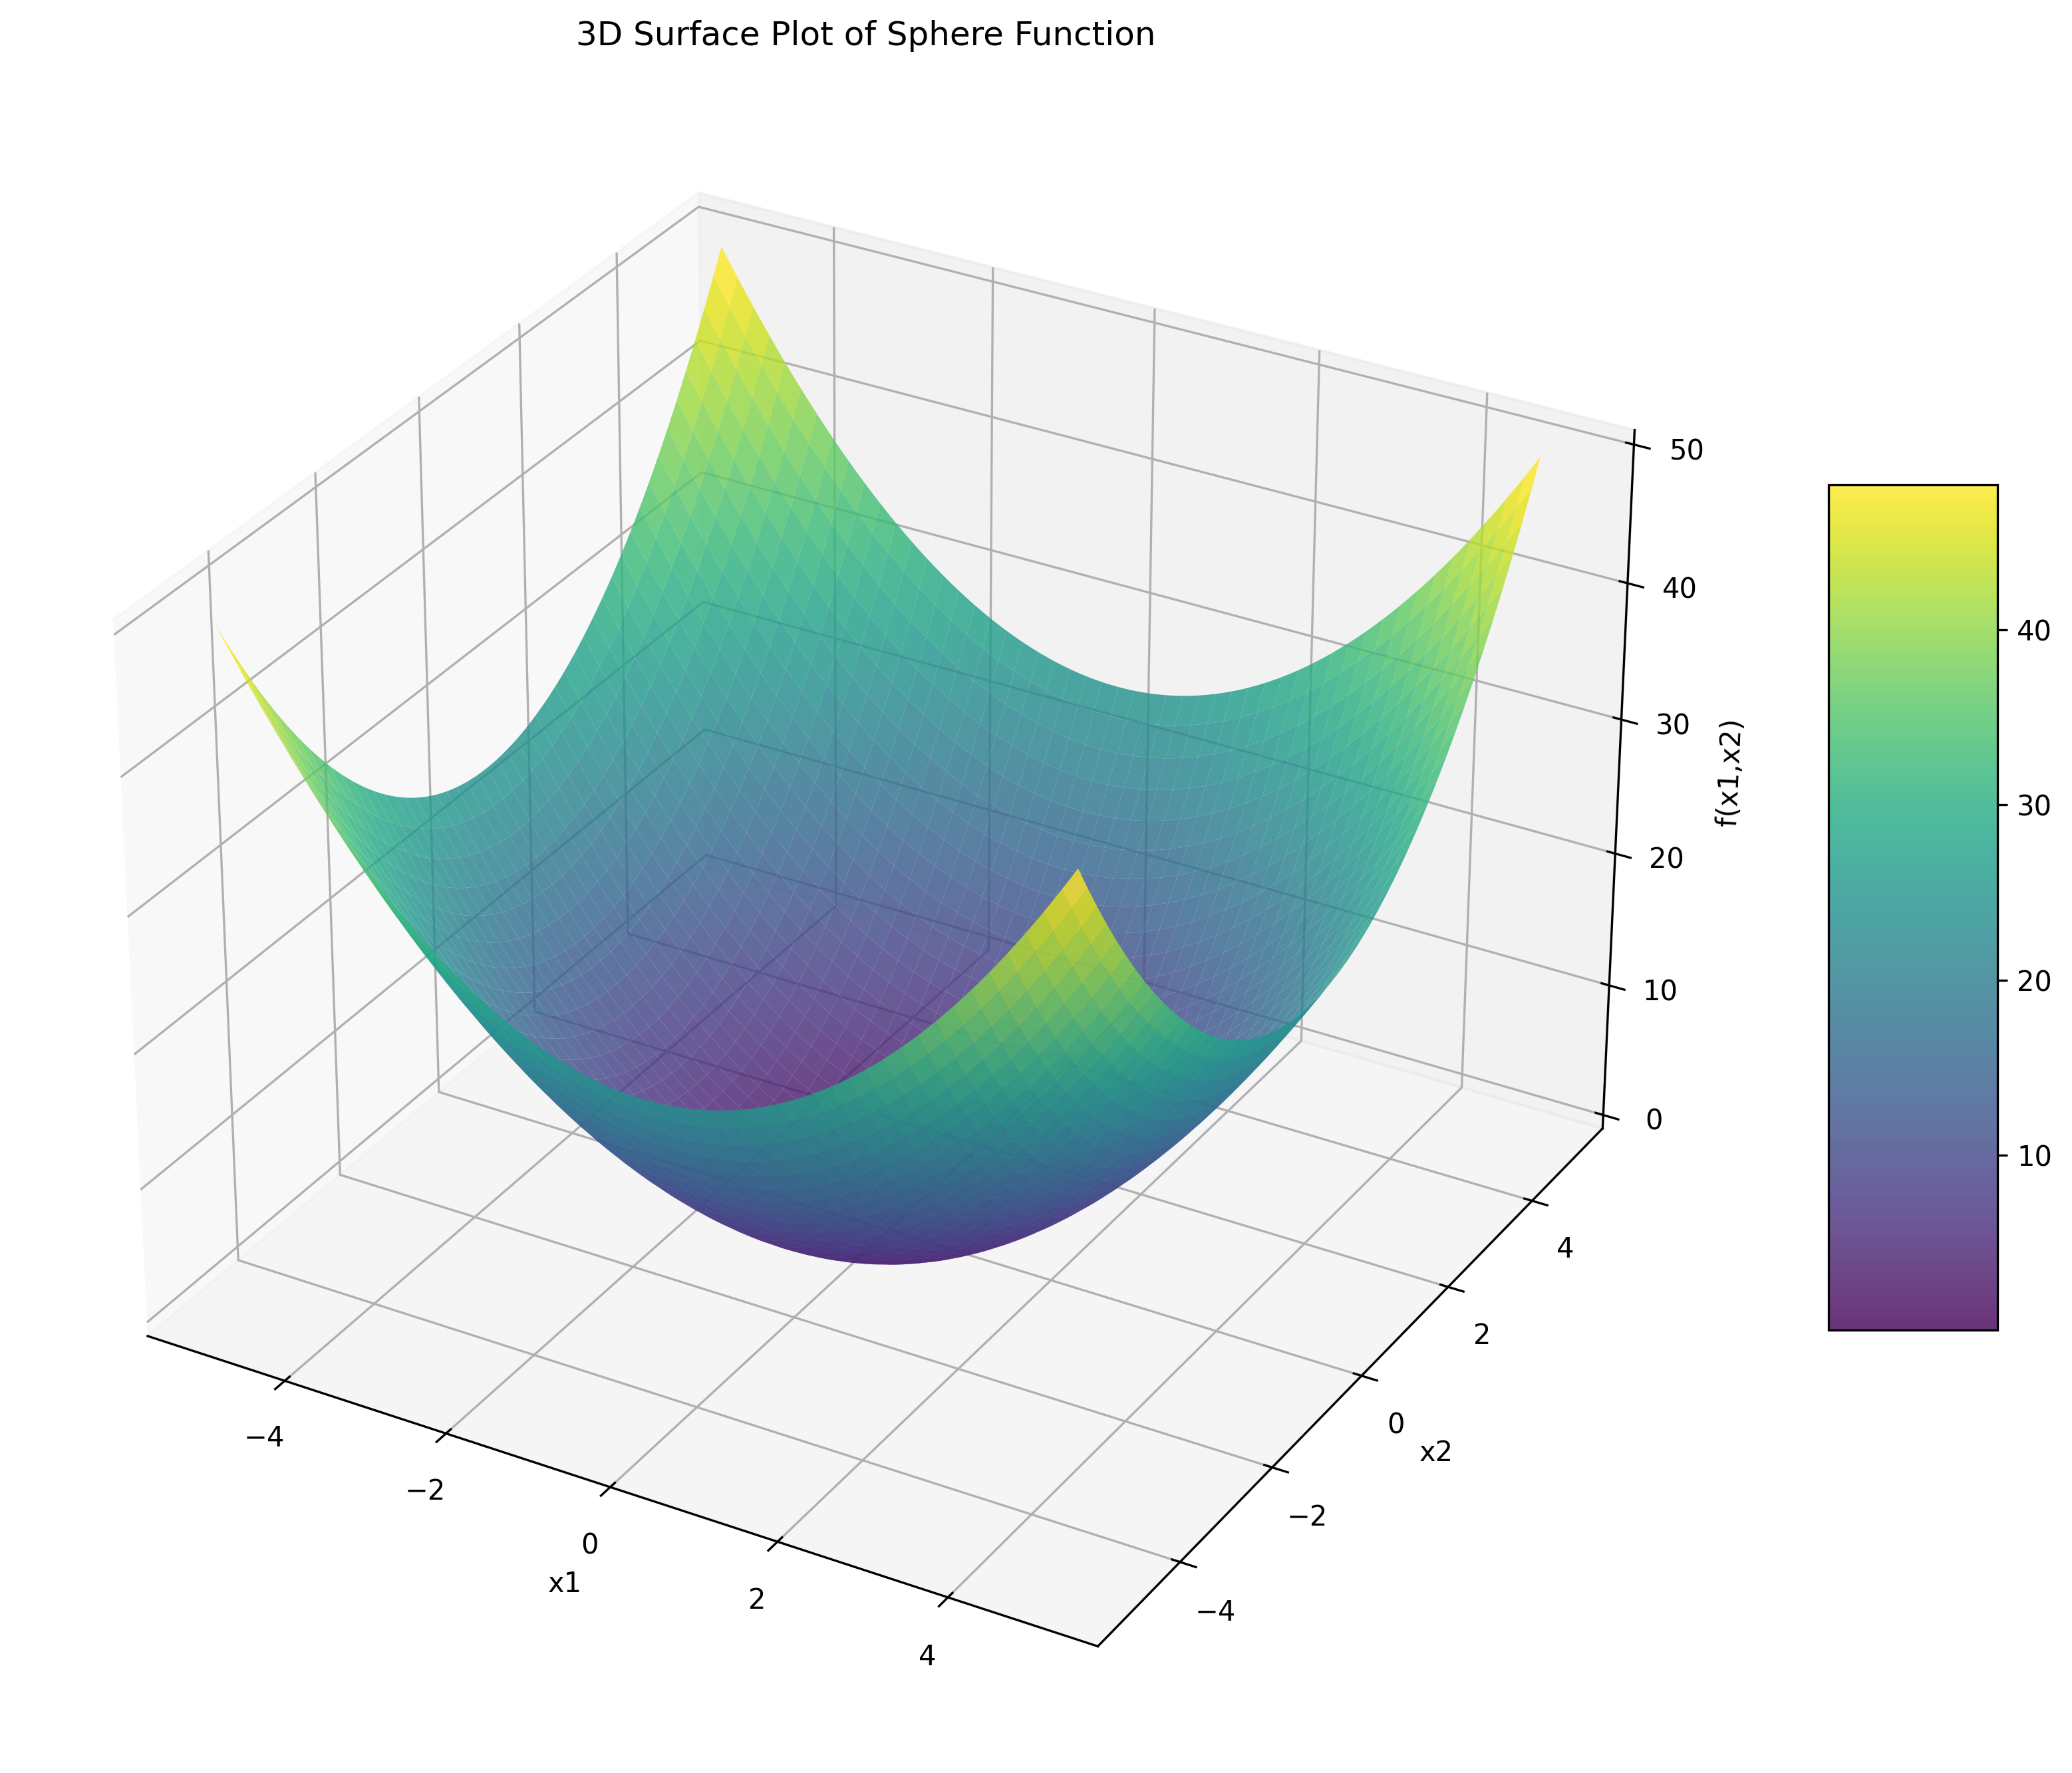
\includegraphics[width=\linewidth]{cec/sphere_3d.png}
		\caption{Dimensi 3}
		\label{fig:sphere-3d}
	\end{subfigure}
	\caption{Tampilan grafik fungsi Sphere pada dimensi dua (\cref{fig:sphere-2d}) dan tiga (\cref{fig:sphere-3d})}
	\label{fig:sphere}
\end{figure}
\begin{flalign*}
  f_{\text{Sphere}}(\mathrm{x})=\sum_{i=1}^{D}z_i^2+f_{\text{bias}}&&
\end{flalign*}

\subsubsection{Step Function}
\noindent Properti:
\begin{packed_item}
  \item unimodal
  \item convex
\end{packed_item}
\begin{figure}[H]
	\centering
	\begin{subfigure}[b]{0.4\textwidth}
		\centering
		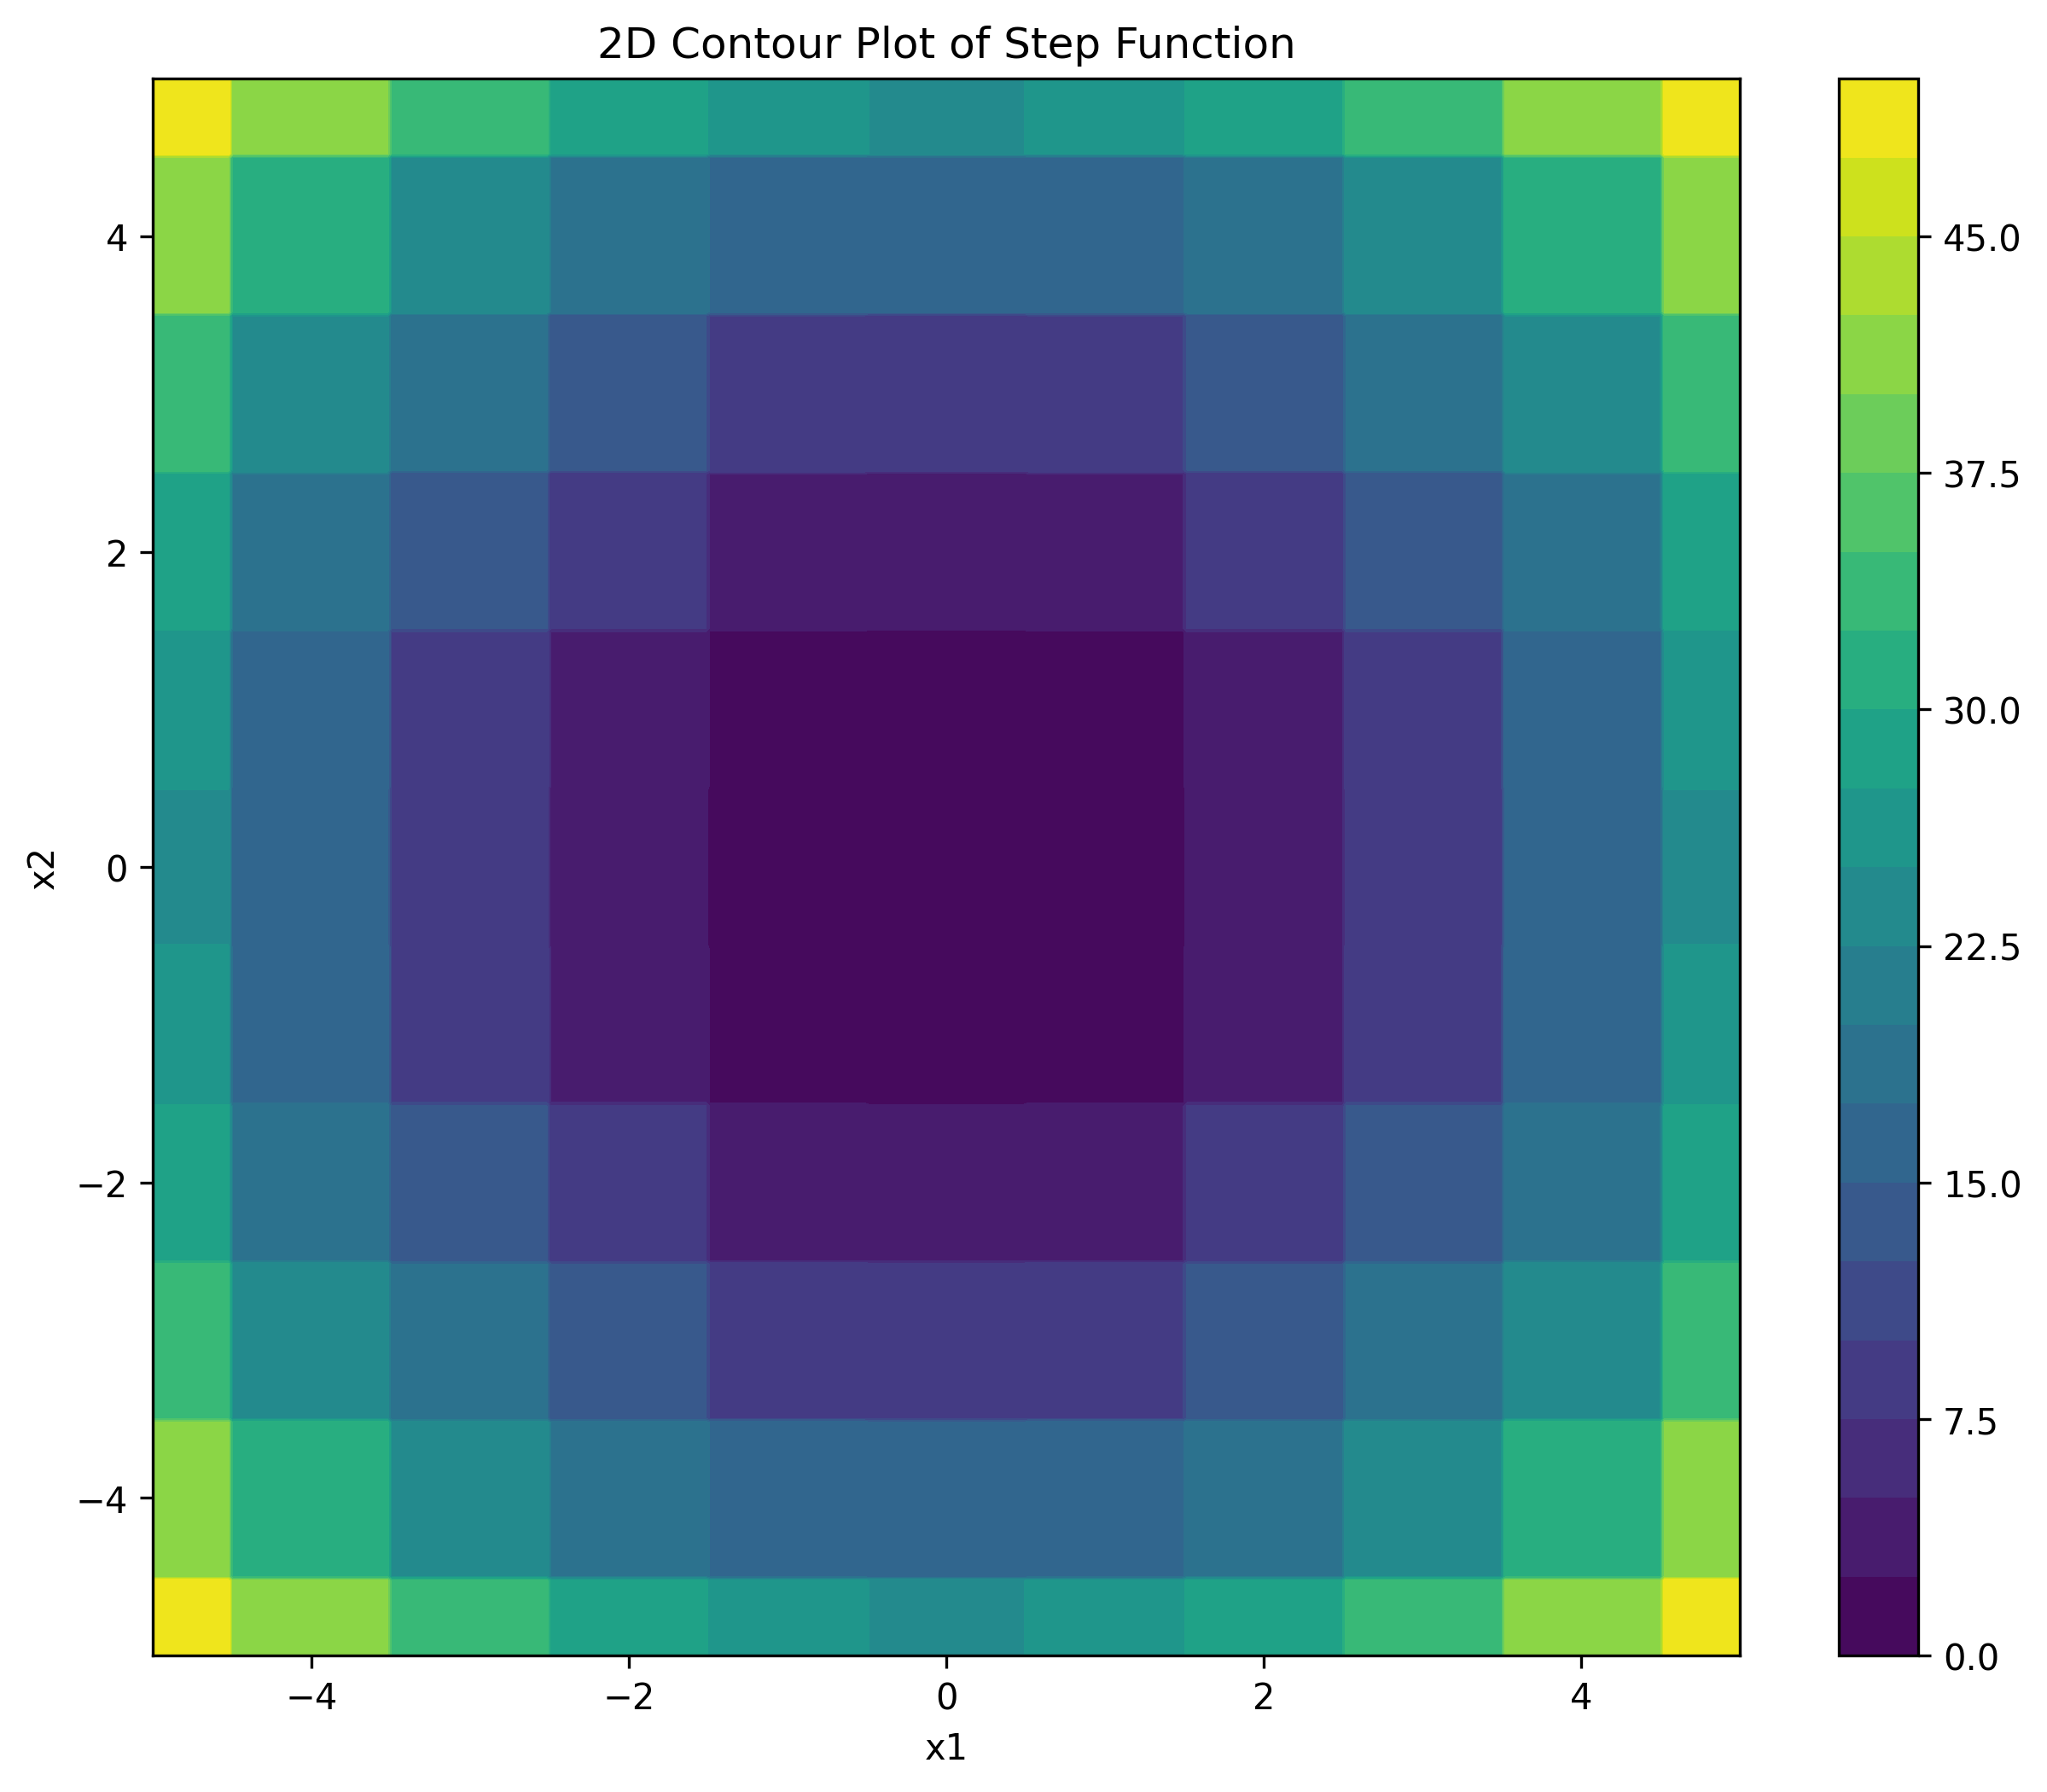
\includegraphics[width=\linewidth]{cec/step_function_2d.png}
		\caption{Dimensi 2}
		\label{fig:step-2d}
	\end{subfigure}
	\hfill
	\begin{subfigure}[b]{0.4\textwidth}
		\centering
		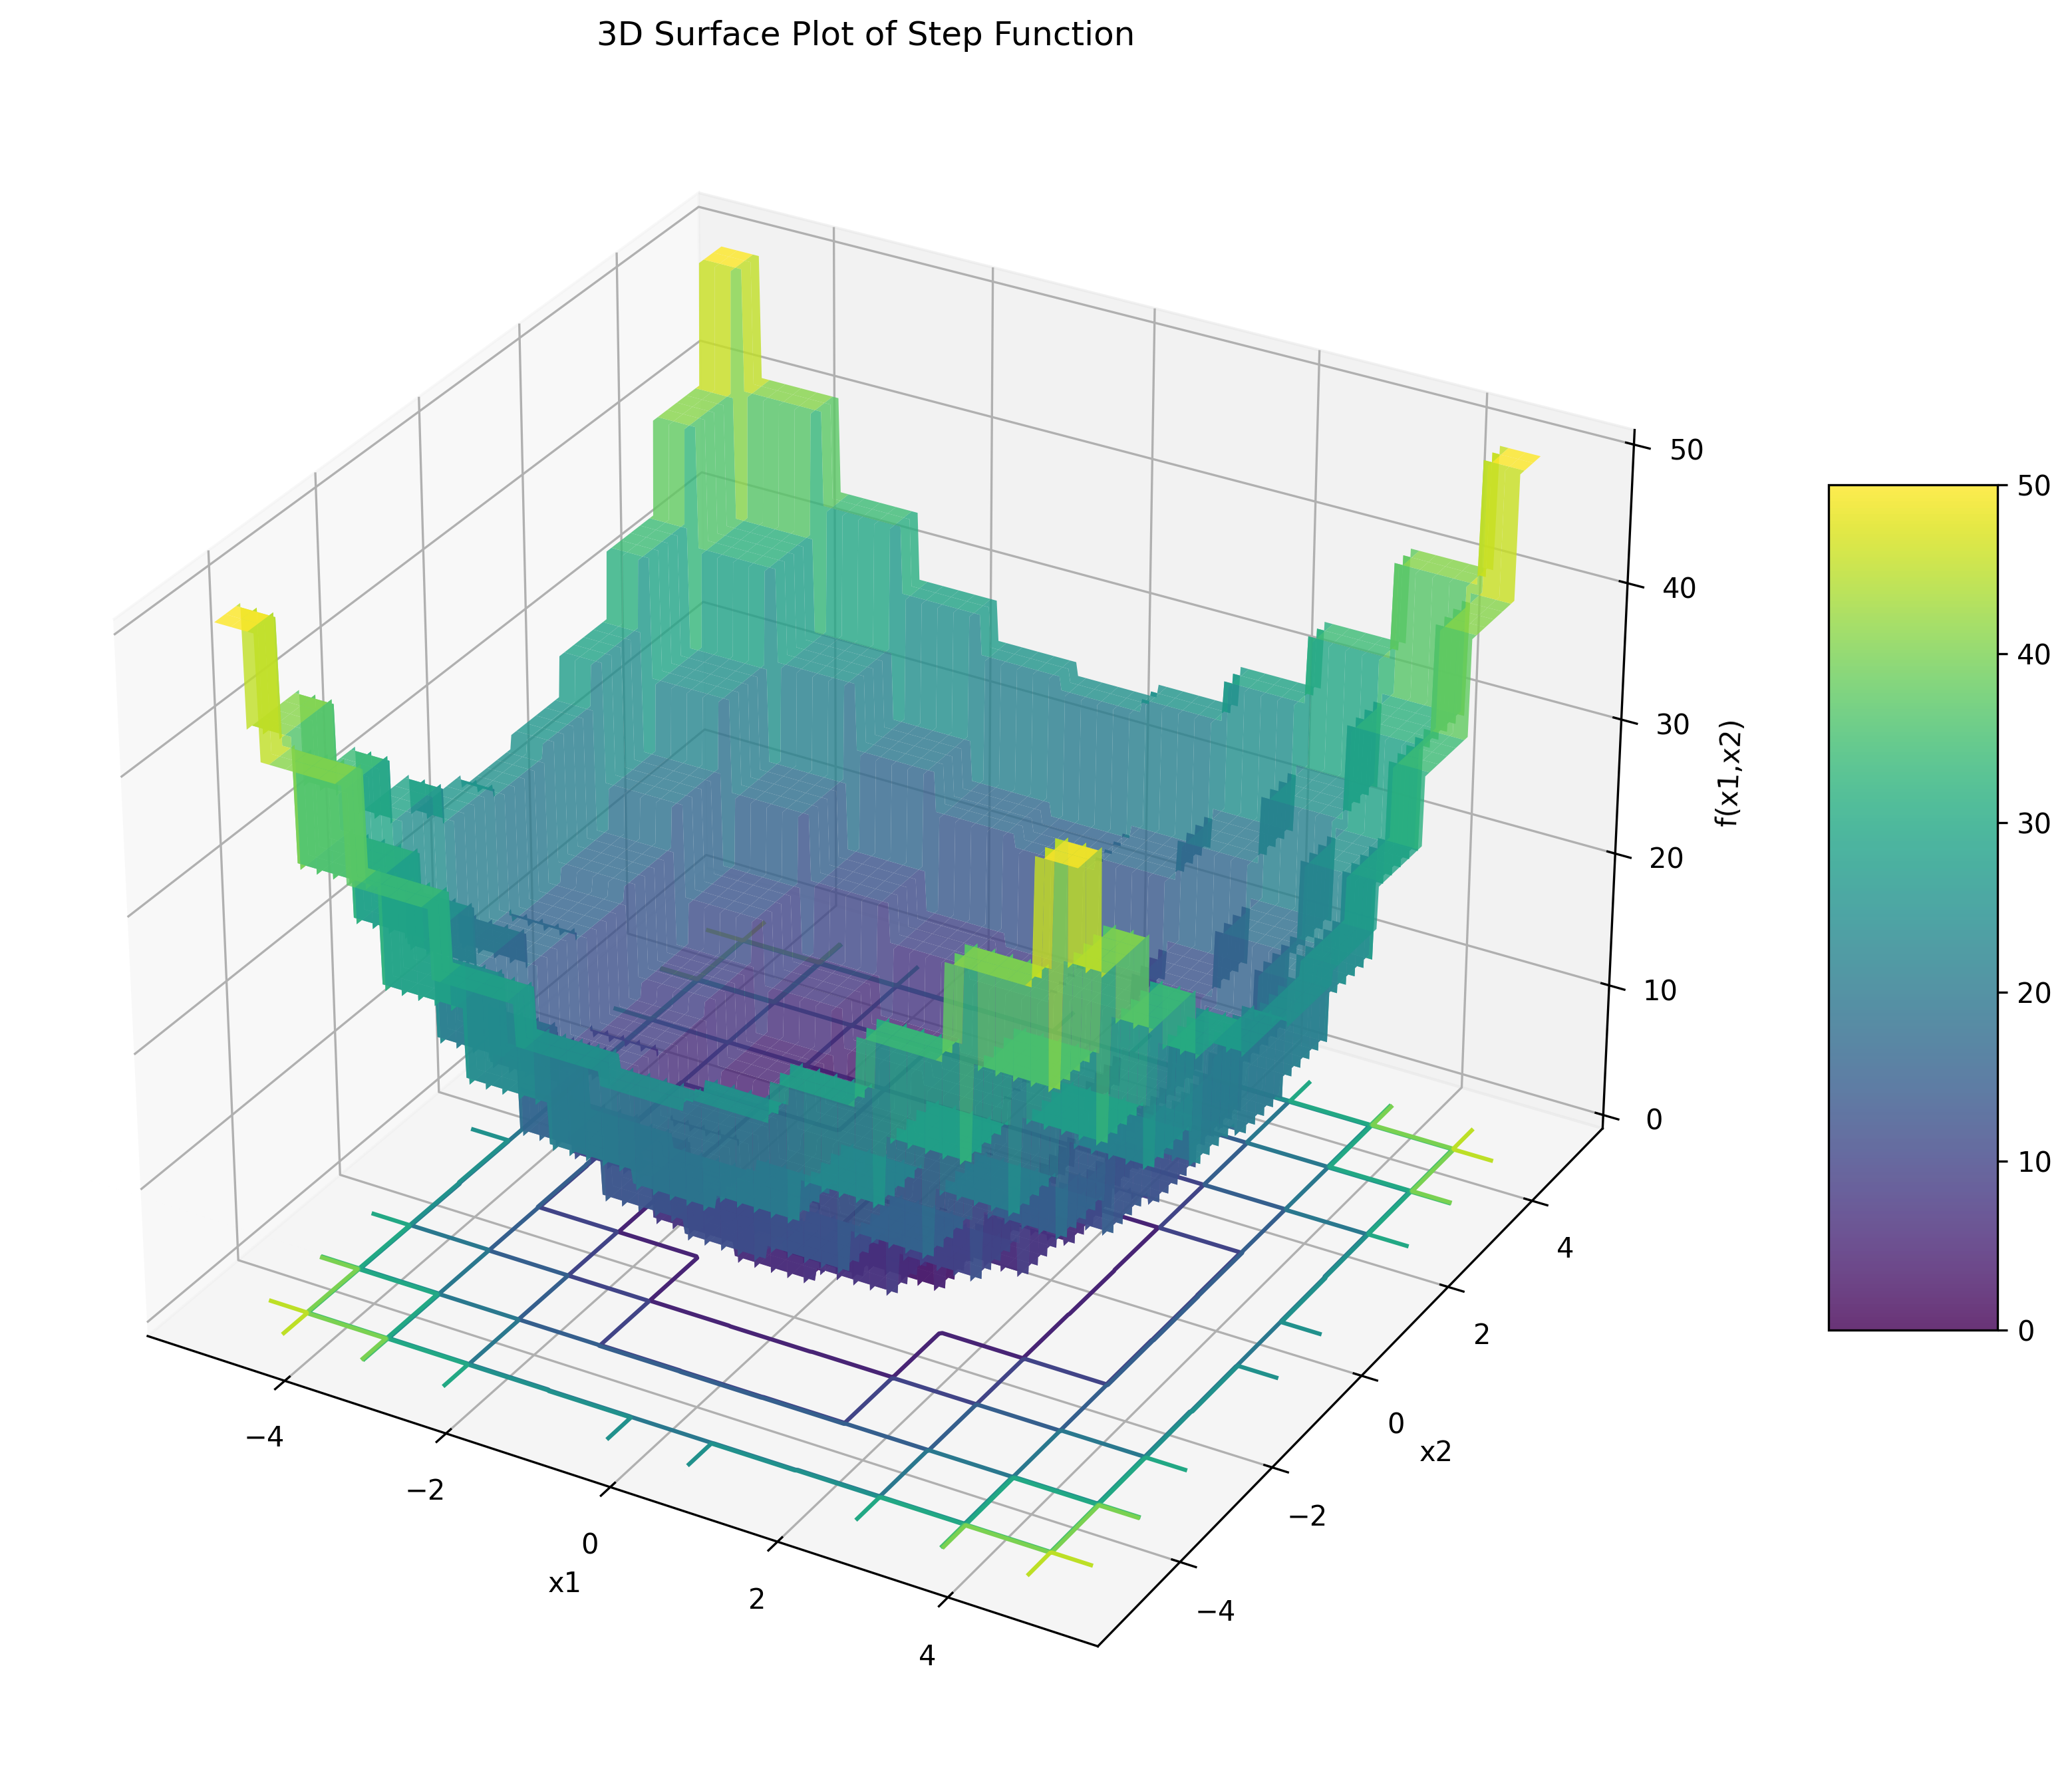
\includegraphics[width=\linewidth]{cec/step_function_3d.png}
		\caption{Dimensi 3}
		\label{fig:step-3d}
	\end{subfigure}
	\caption{Tampilan grafik fungsi Step Function pada dimensi dua (\cref{fig:step-2d}) dan tiga (\cref{fig:step-3d})}
	\label{fig:step-function}
\end{figure}
\begin{flalign*}
  f_{\text{Step function}}(\mathrm{x})=\sum_{i=1}^{D}\left(\left\lfloor z_i + 0.5 \right\rfloor \right)^2+f_{\text{bias}}&&
\end{flalign*}

\subsubsection{Vincent}
\noindent Properti:
\begin{packed_item}
  \item multimodal
  \item non-convex
\end{packed_item}
\begin{figure}[H]
	\centering
	\begin{subfigure}[b]{0.4\textwidth}
		\centering
		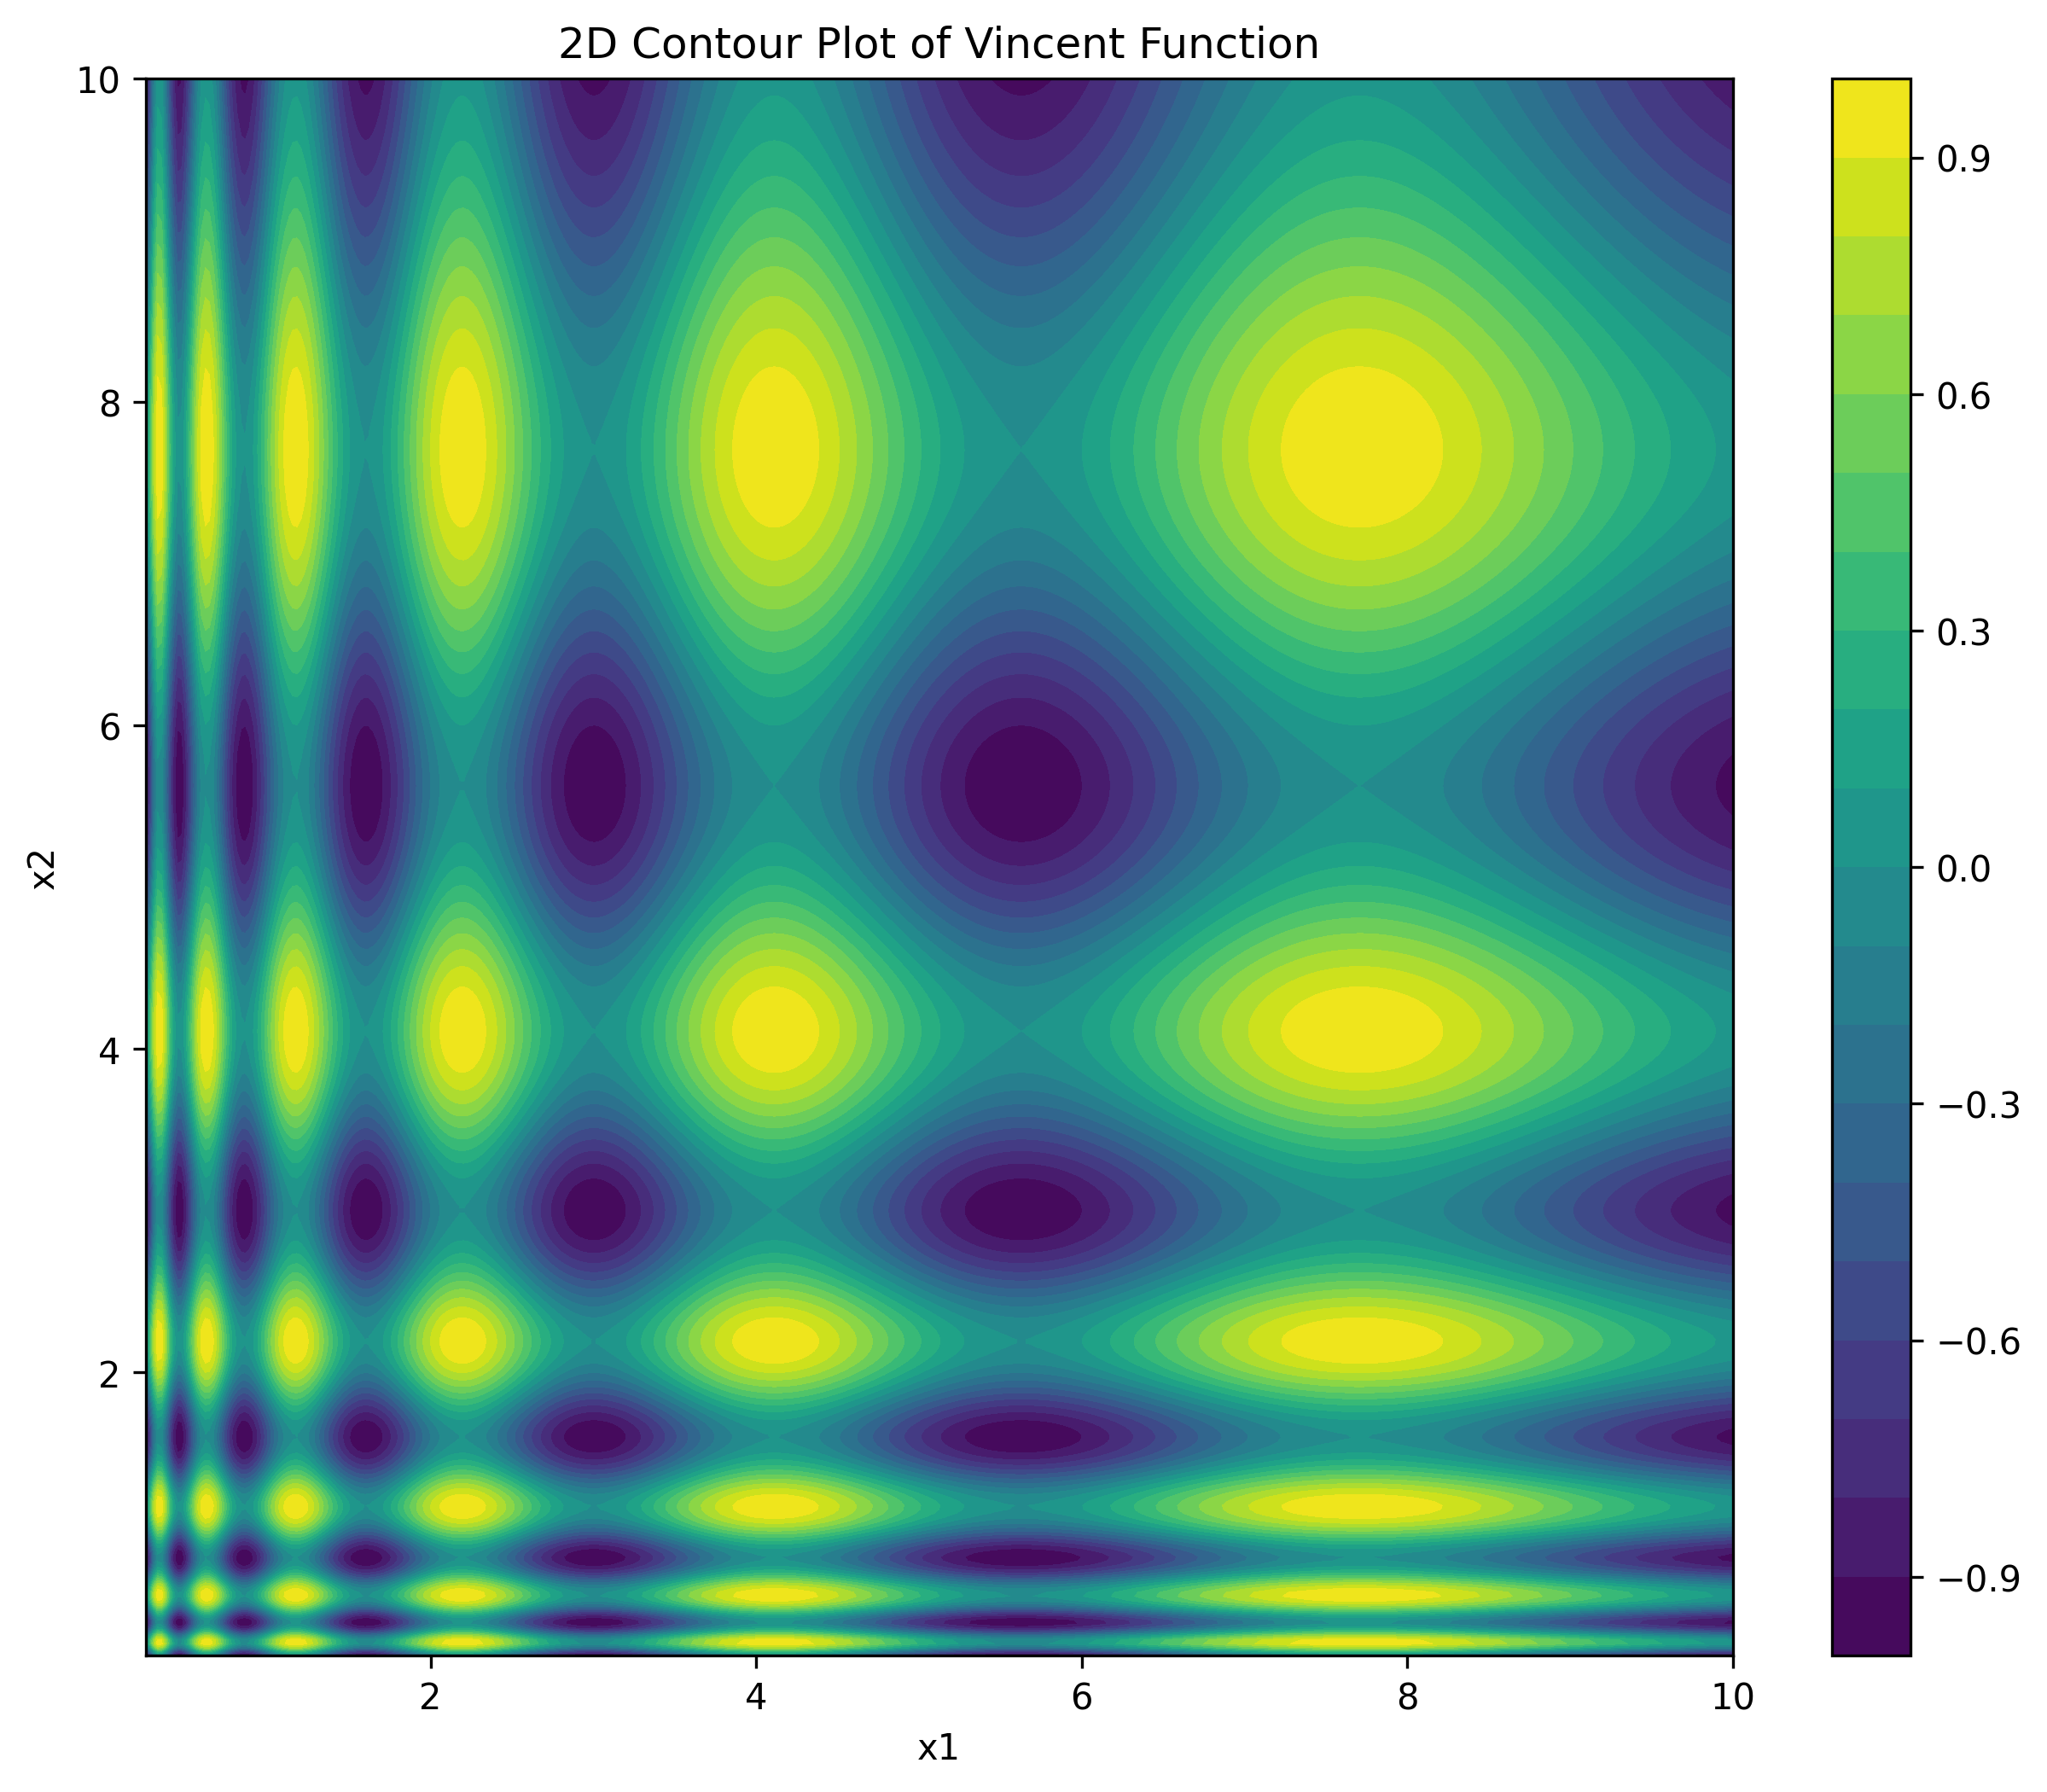
\includegraphics[width=\linewidth]{cec/vincent_2d.png}
		\caption{Dimensi 2}
		\label{fig:vincent-2d}
	\end{subfigure}
	\hfill
	\begin{subfigure}[b]{0.4\textwidth}
		\centering
		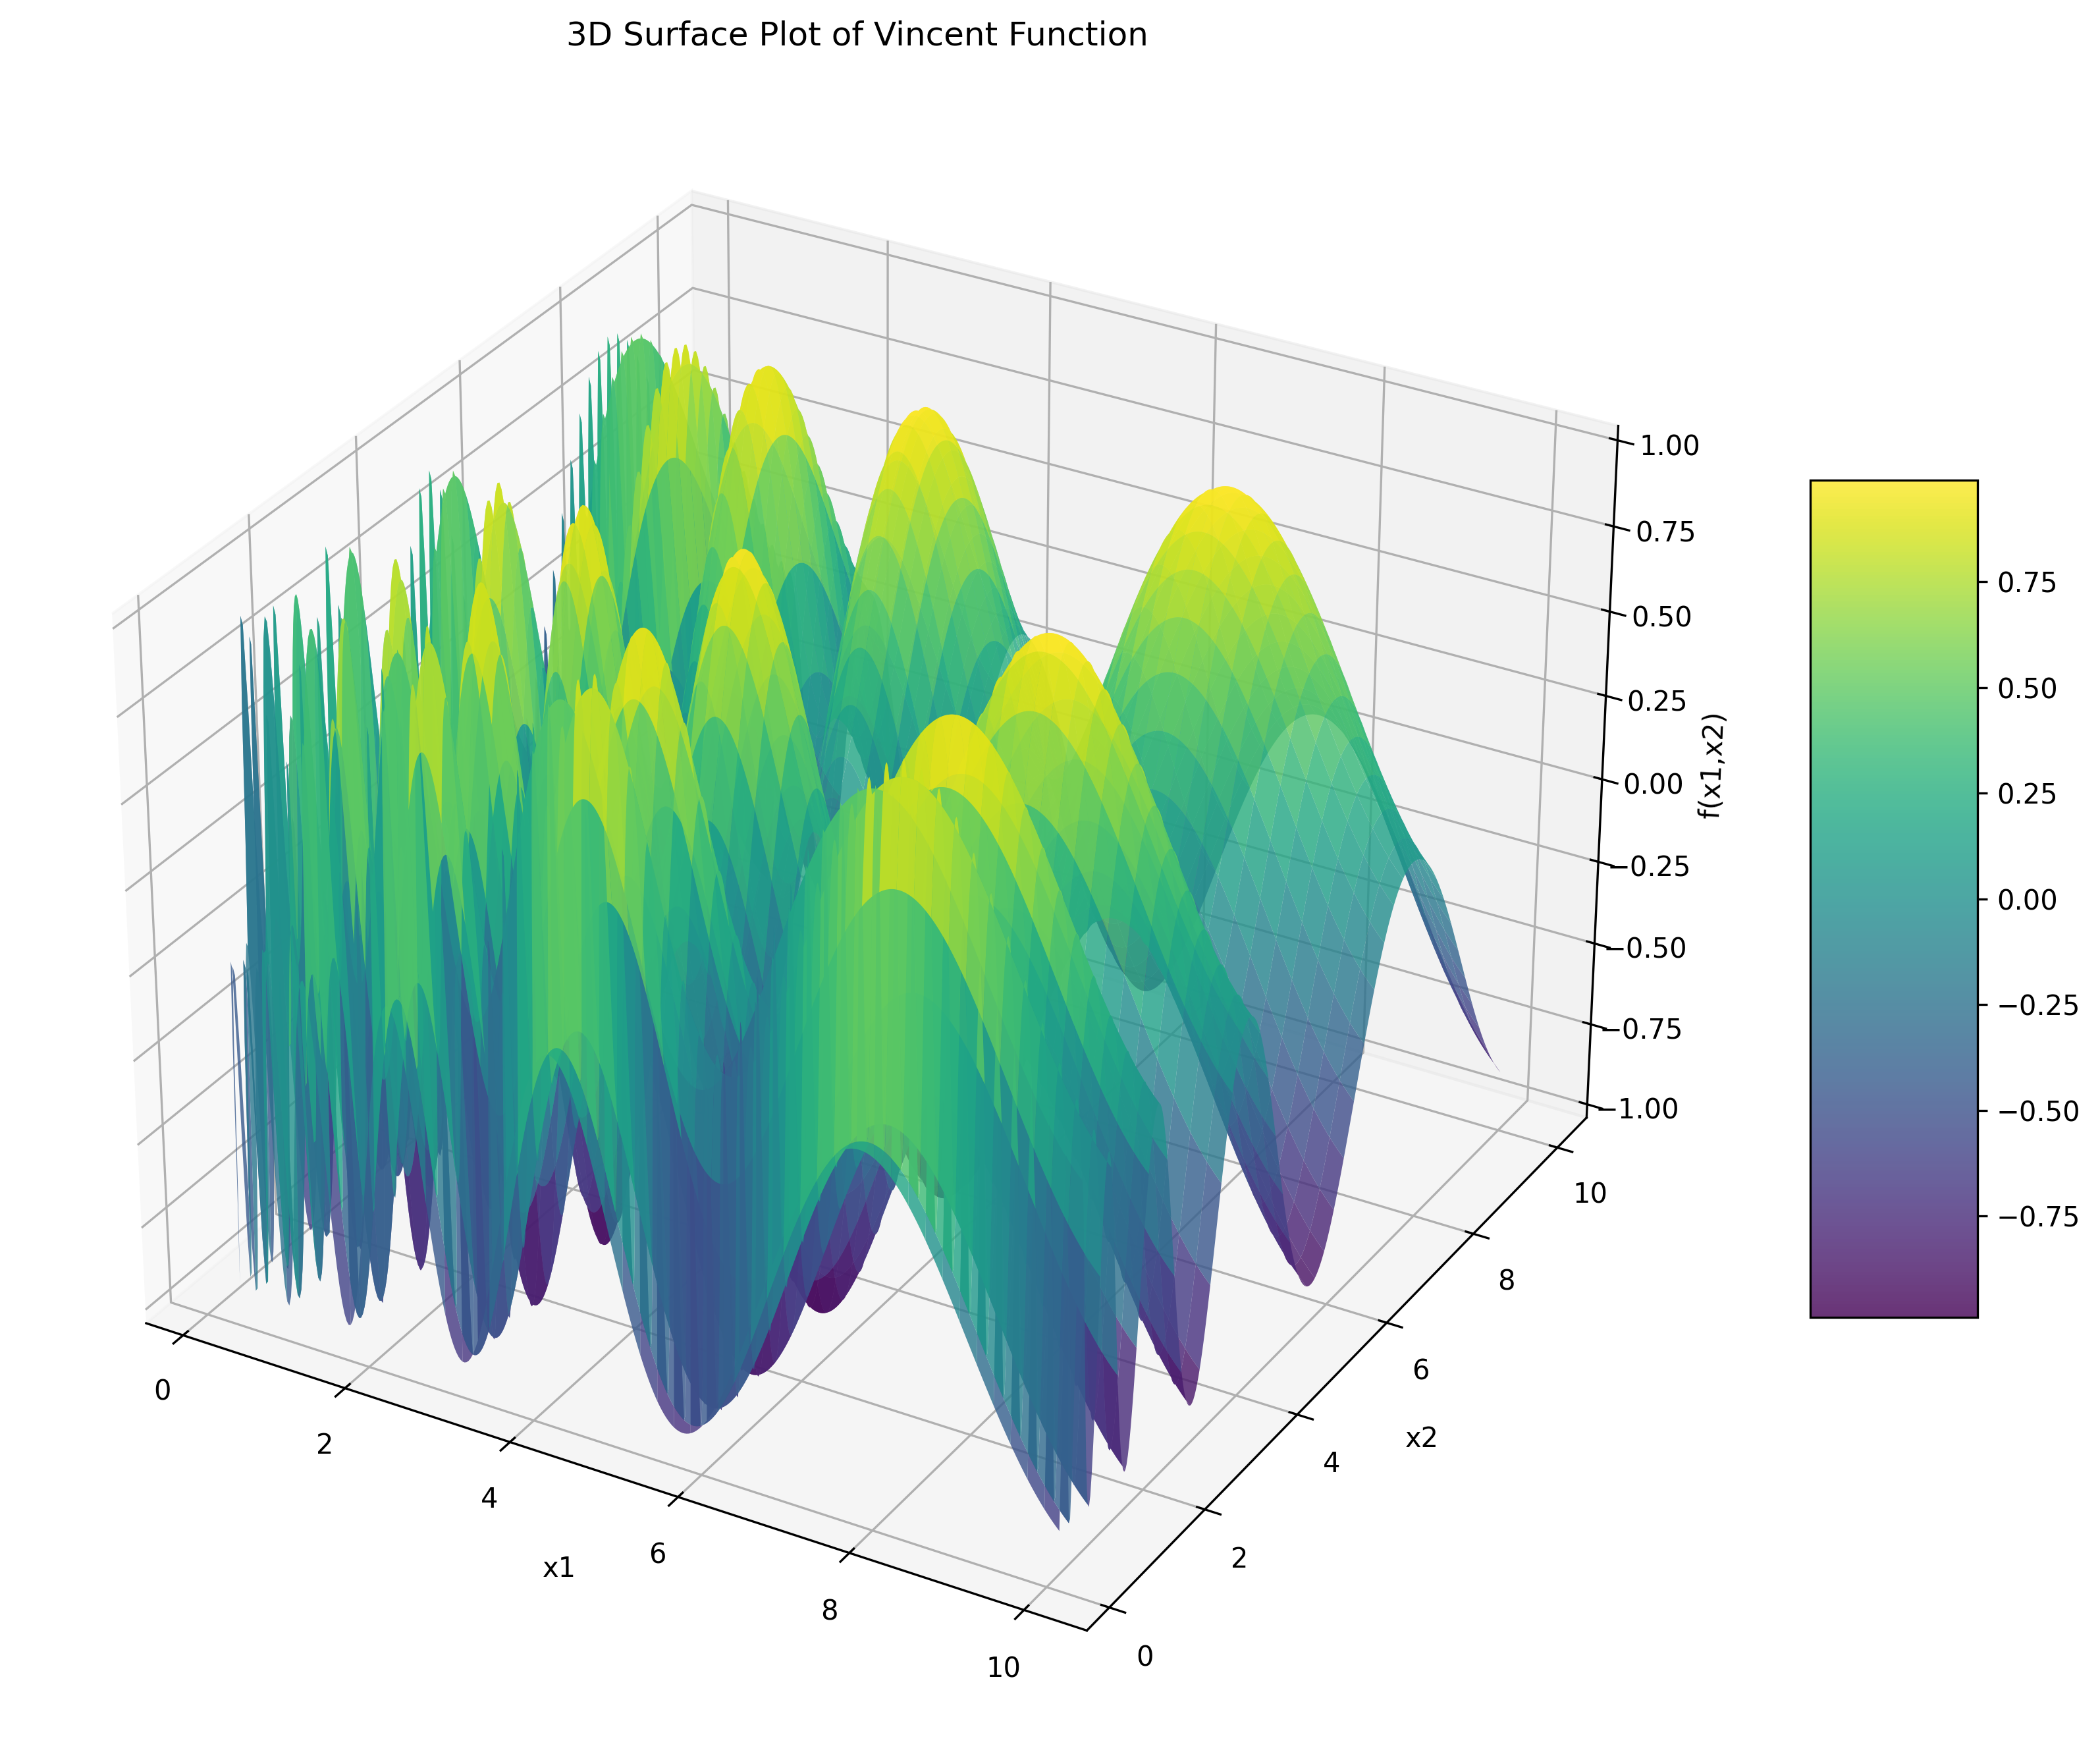
\includegraphics[width=\linewidth]{cec/vincent_3d.png}
		\caption{Dimensi 3}
		\label{fig:vincent-3d}
	\end{subfigure}
	\caption{Tampilan grafik fungsi Vincent pada dimensi dua (\cref{fig:vincent-2d}) dan tiga (\cref{fig:vincent-3d})}
	\label{fig:vincent}
\end{figure}
\begin{flalign*}
  f_{\text{Vincent}}(\mathrm{x})=\frac{1}{D}\sum_{i=1}^{D}\sin\left(10 \log\left(z_i \right)  \right) +f_{\text{bias}}&&
\end{flalign*}

\subsubsection{Weierstrass}
\noindent Properti:
\begin{packed_item}
  \item multimodal
  \item non-convex
  \item non-separable
  \item Continuous but differentiable only on a set of points
\end{packed_item}
\begin{figure}[H]
	\centering
	\begin{subfigure}[b]{0.4\textwidth}
		\centering
		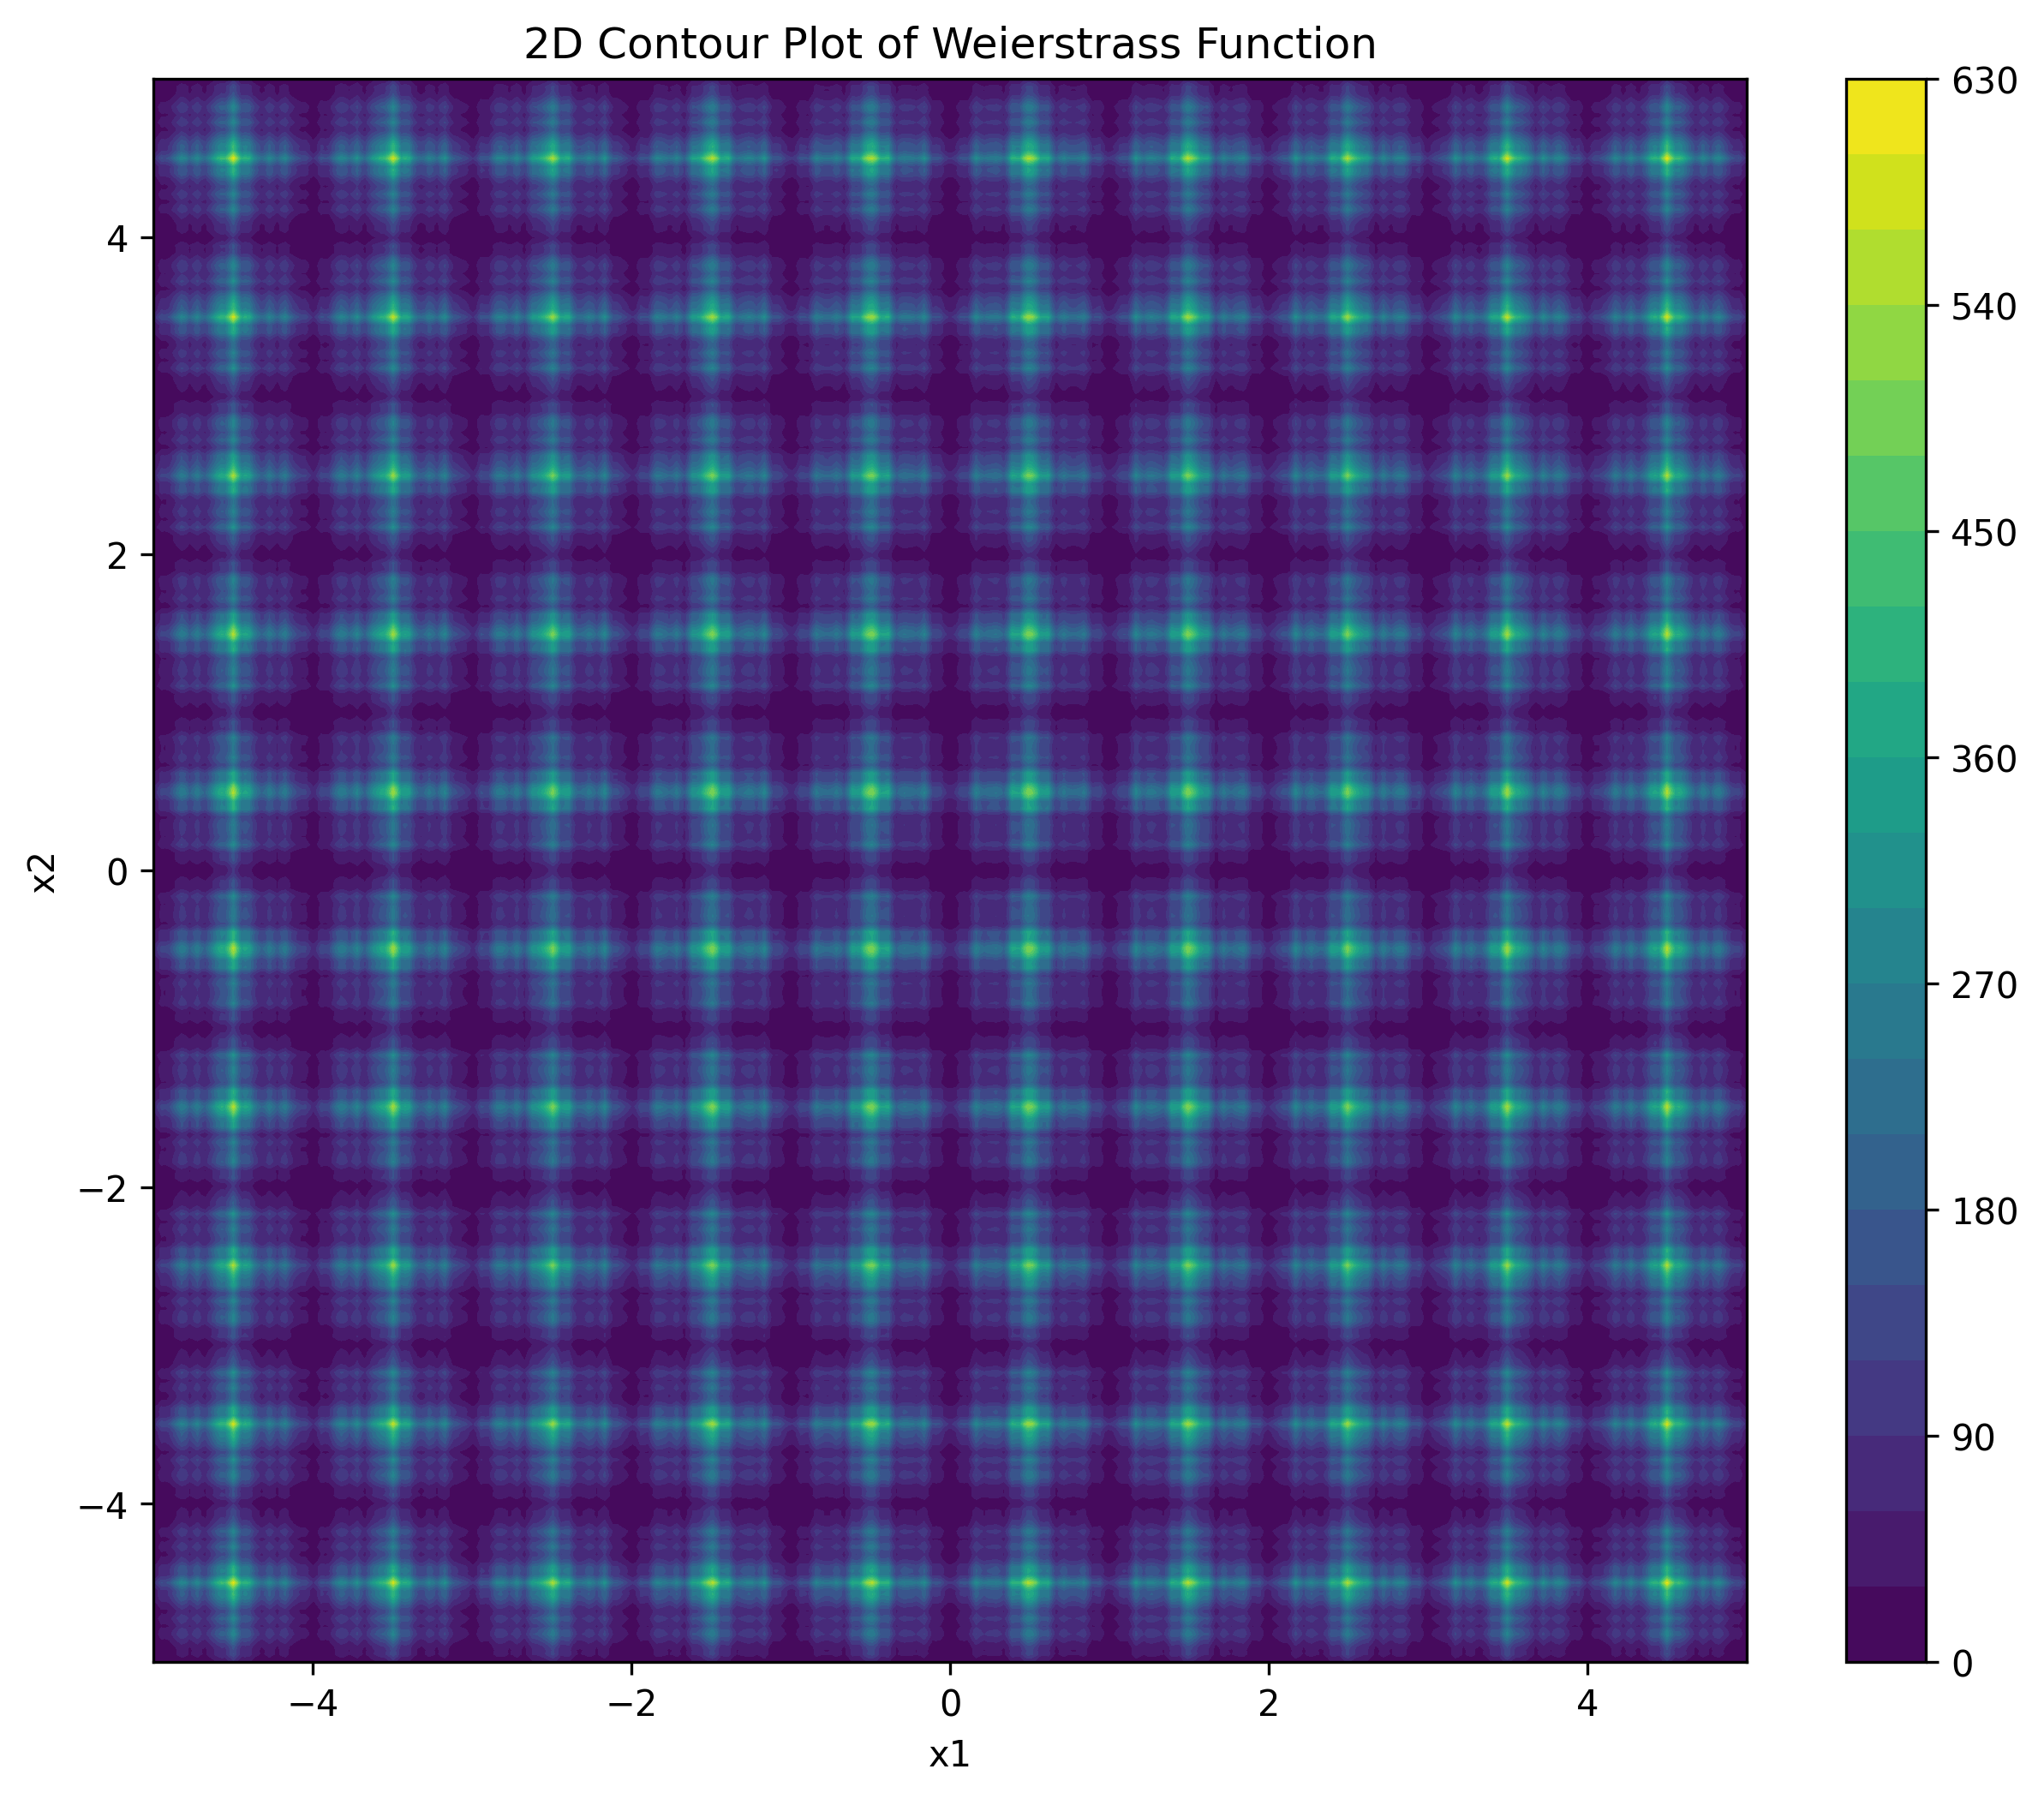
\includegraphics[width=\linewidth]{cec/weierstrass_2d.png}
		\caption{Dimensi 2}
		\label{fig:weierstrass-2d}
	\end{subfigure}
	\hfill
	\begin{subfigure}[b]{0.4\textwidth}
		\centering
		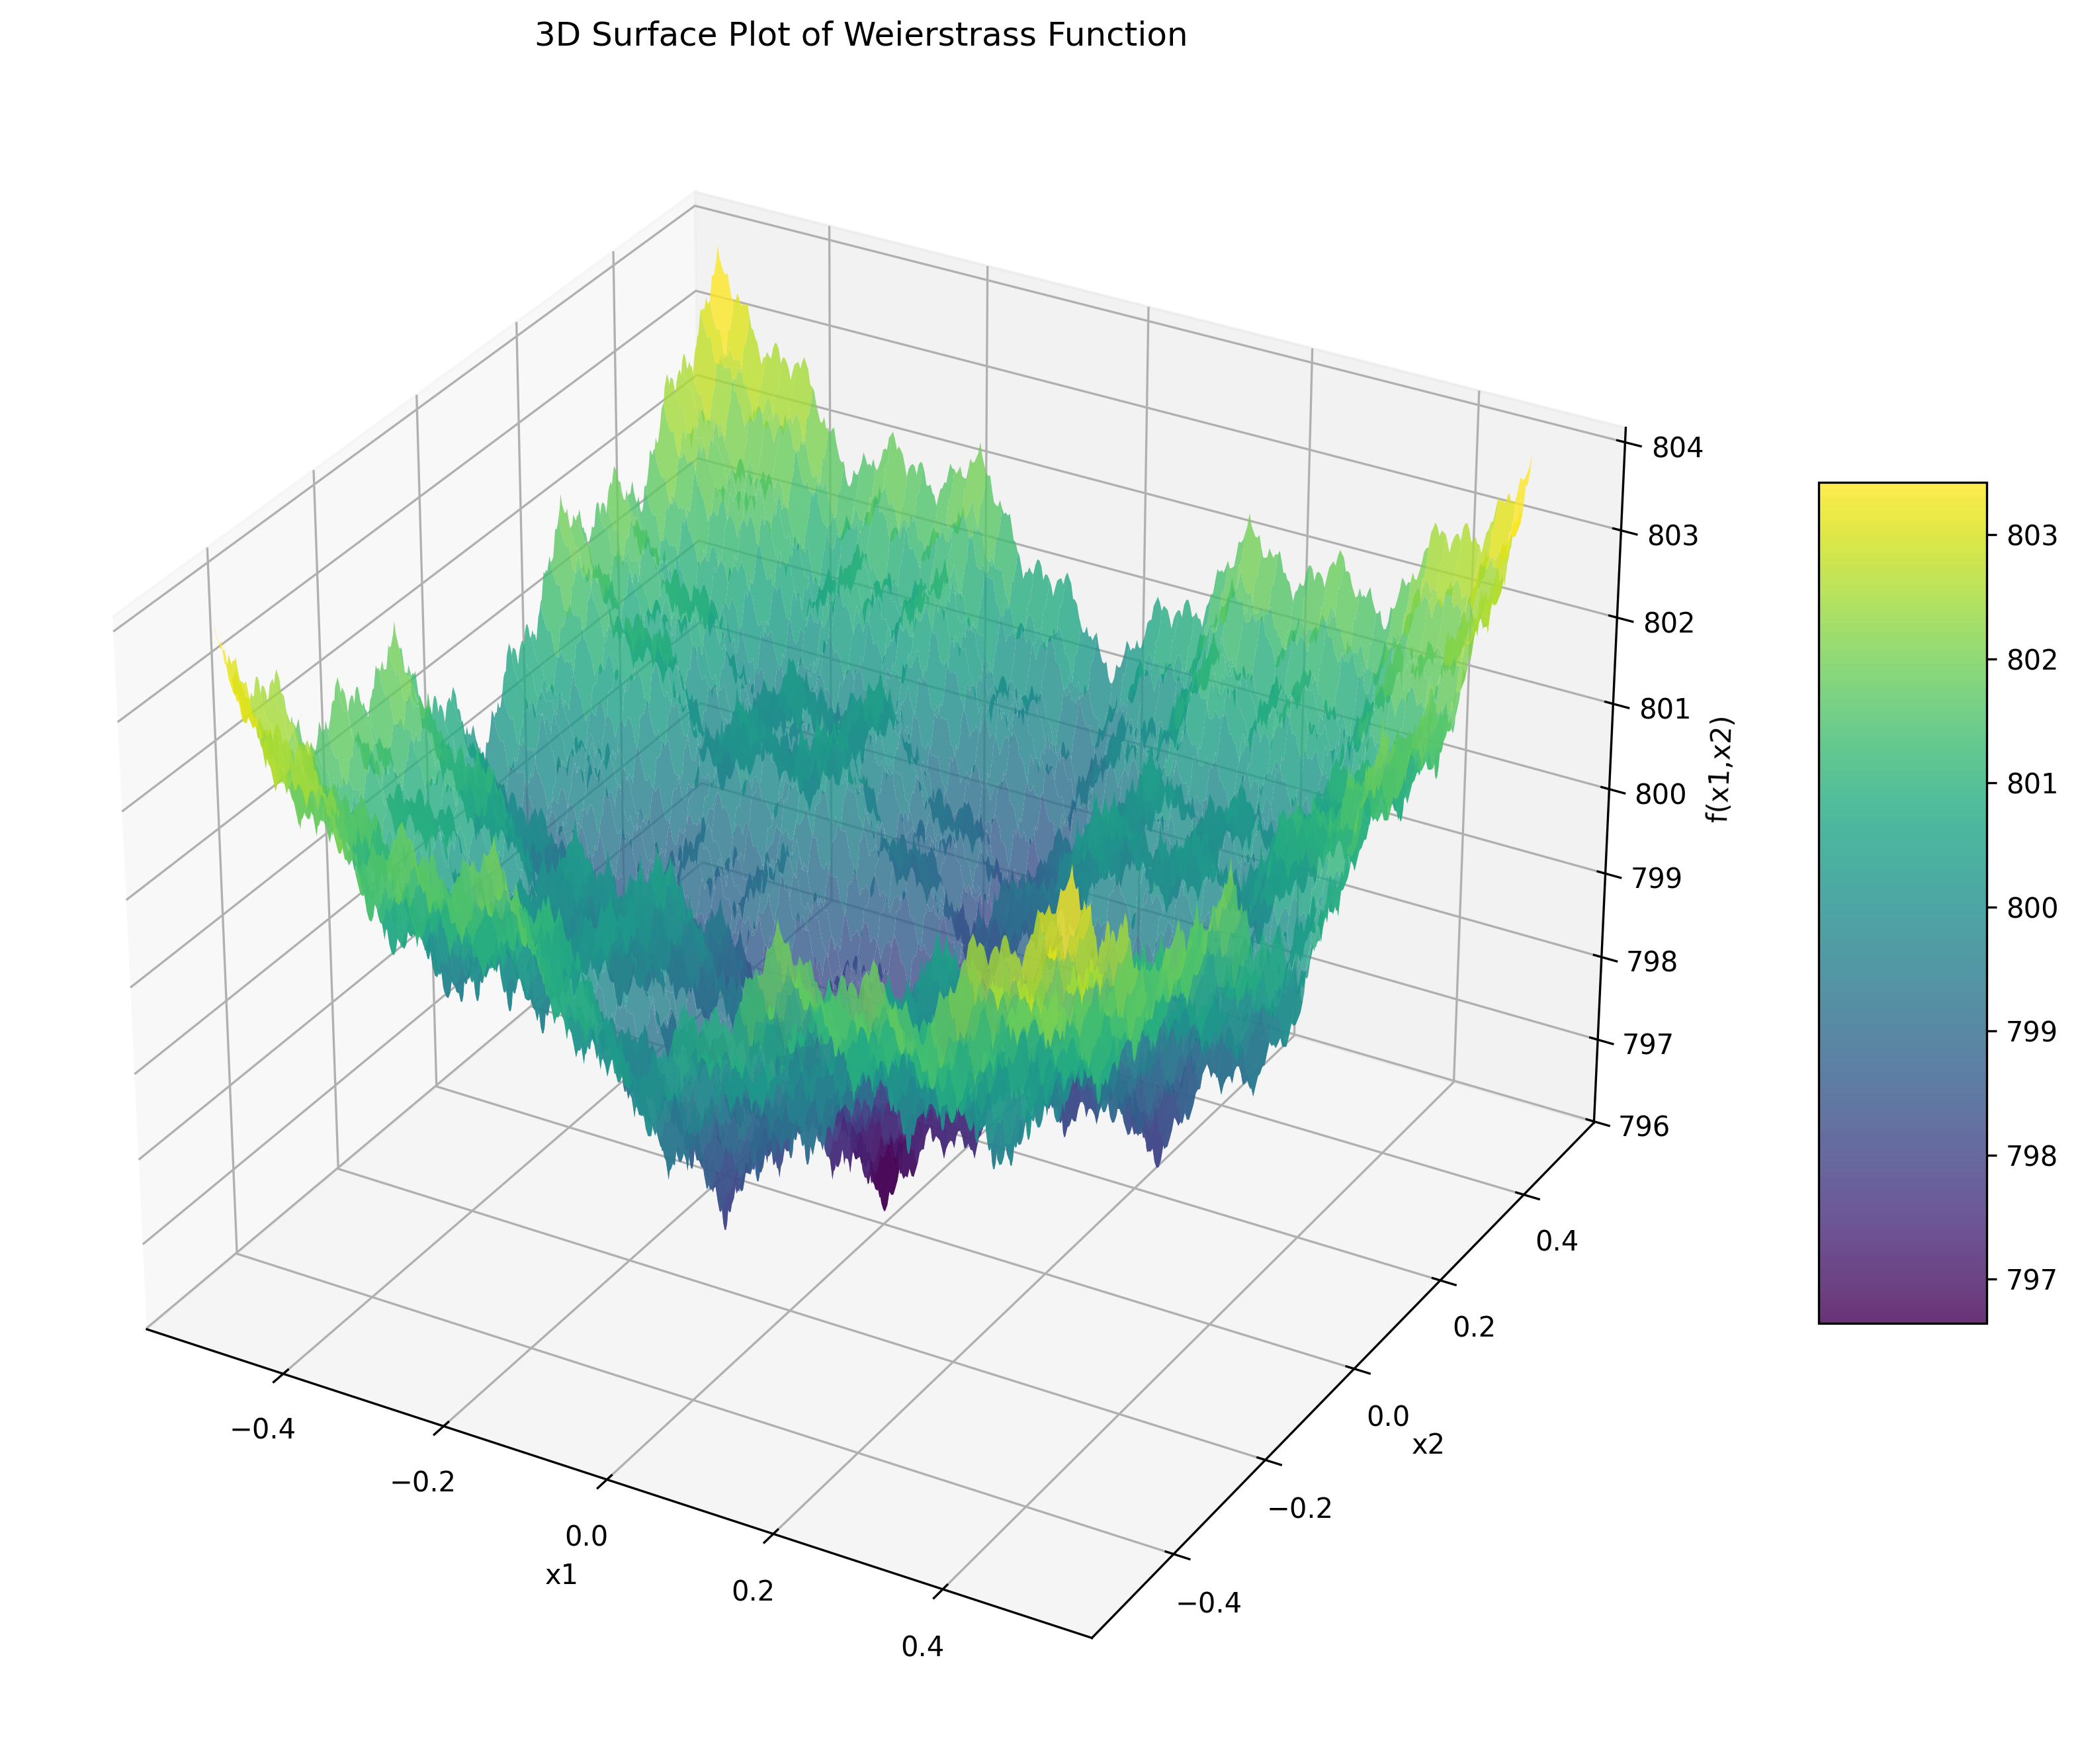
\includegraphics[width=\linewidth]{cec/weierstrass_3d.png}
		\caption{Dimensi 3}
		\label{fig:weierstrass-3d}
	\end{subfigure}
	\caption{Tampilan grafik fungsi Weierstrass pada dimensi dua (\cref{fig:weierstrass-2d}) dan tiga (\cref{fig:weierstrass-3d})}
	\label{fig:weierstrass}
\end{figure}
\begin{align*}
  f_{\text{Weierstrass}}(\mathrm{x})=\sum_{i=1}^{D}\left(\sum_{k=0}^{k\ \text{max}}\left[a^k\cos\left(2\pi b^k\left( z_i+0.5\right)  \right)  \right]  \right)-D\sum_{i=0}^{k \text{max}}\left[ a^k\cos\left(2\pi b^k\cdot0.5 \right) \right]  +f_{\text{bias}}&&
\end{align*}

\subsubsection{Zakharov}
\noindent Properti:
\begin{packed_item}
  \item unimodal
  \item convex
  \item non-separable
\end{packed_item}
\begin{figure}[H]
	\centering
	\begin{subfigure}[b]{0.4\textwidth}
		\centering
		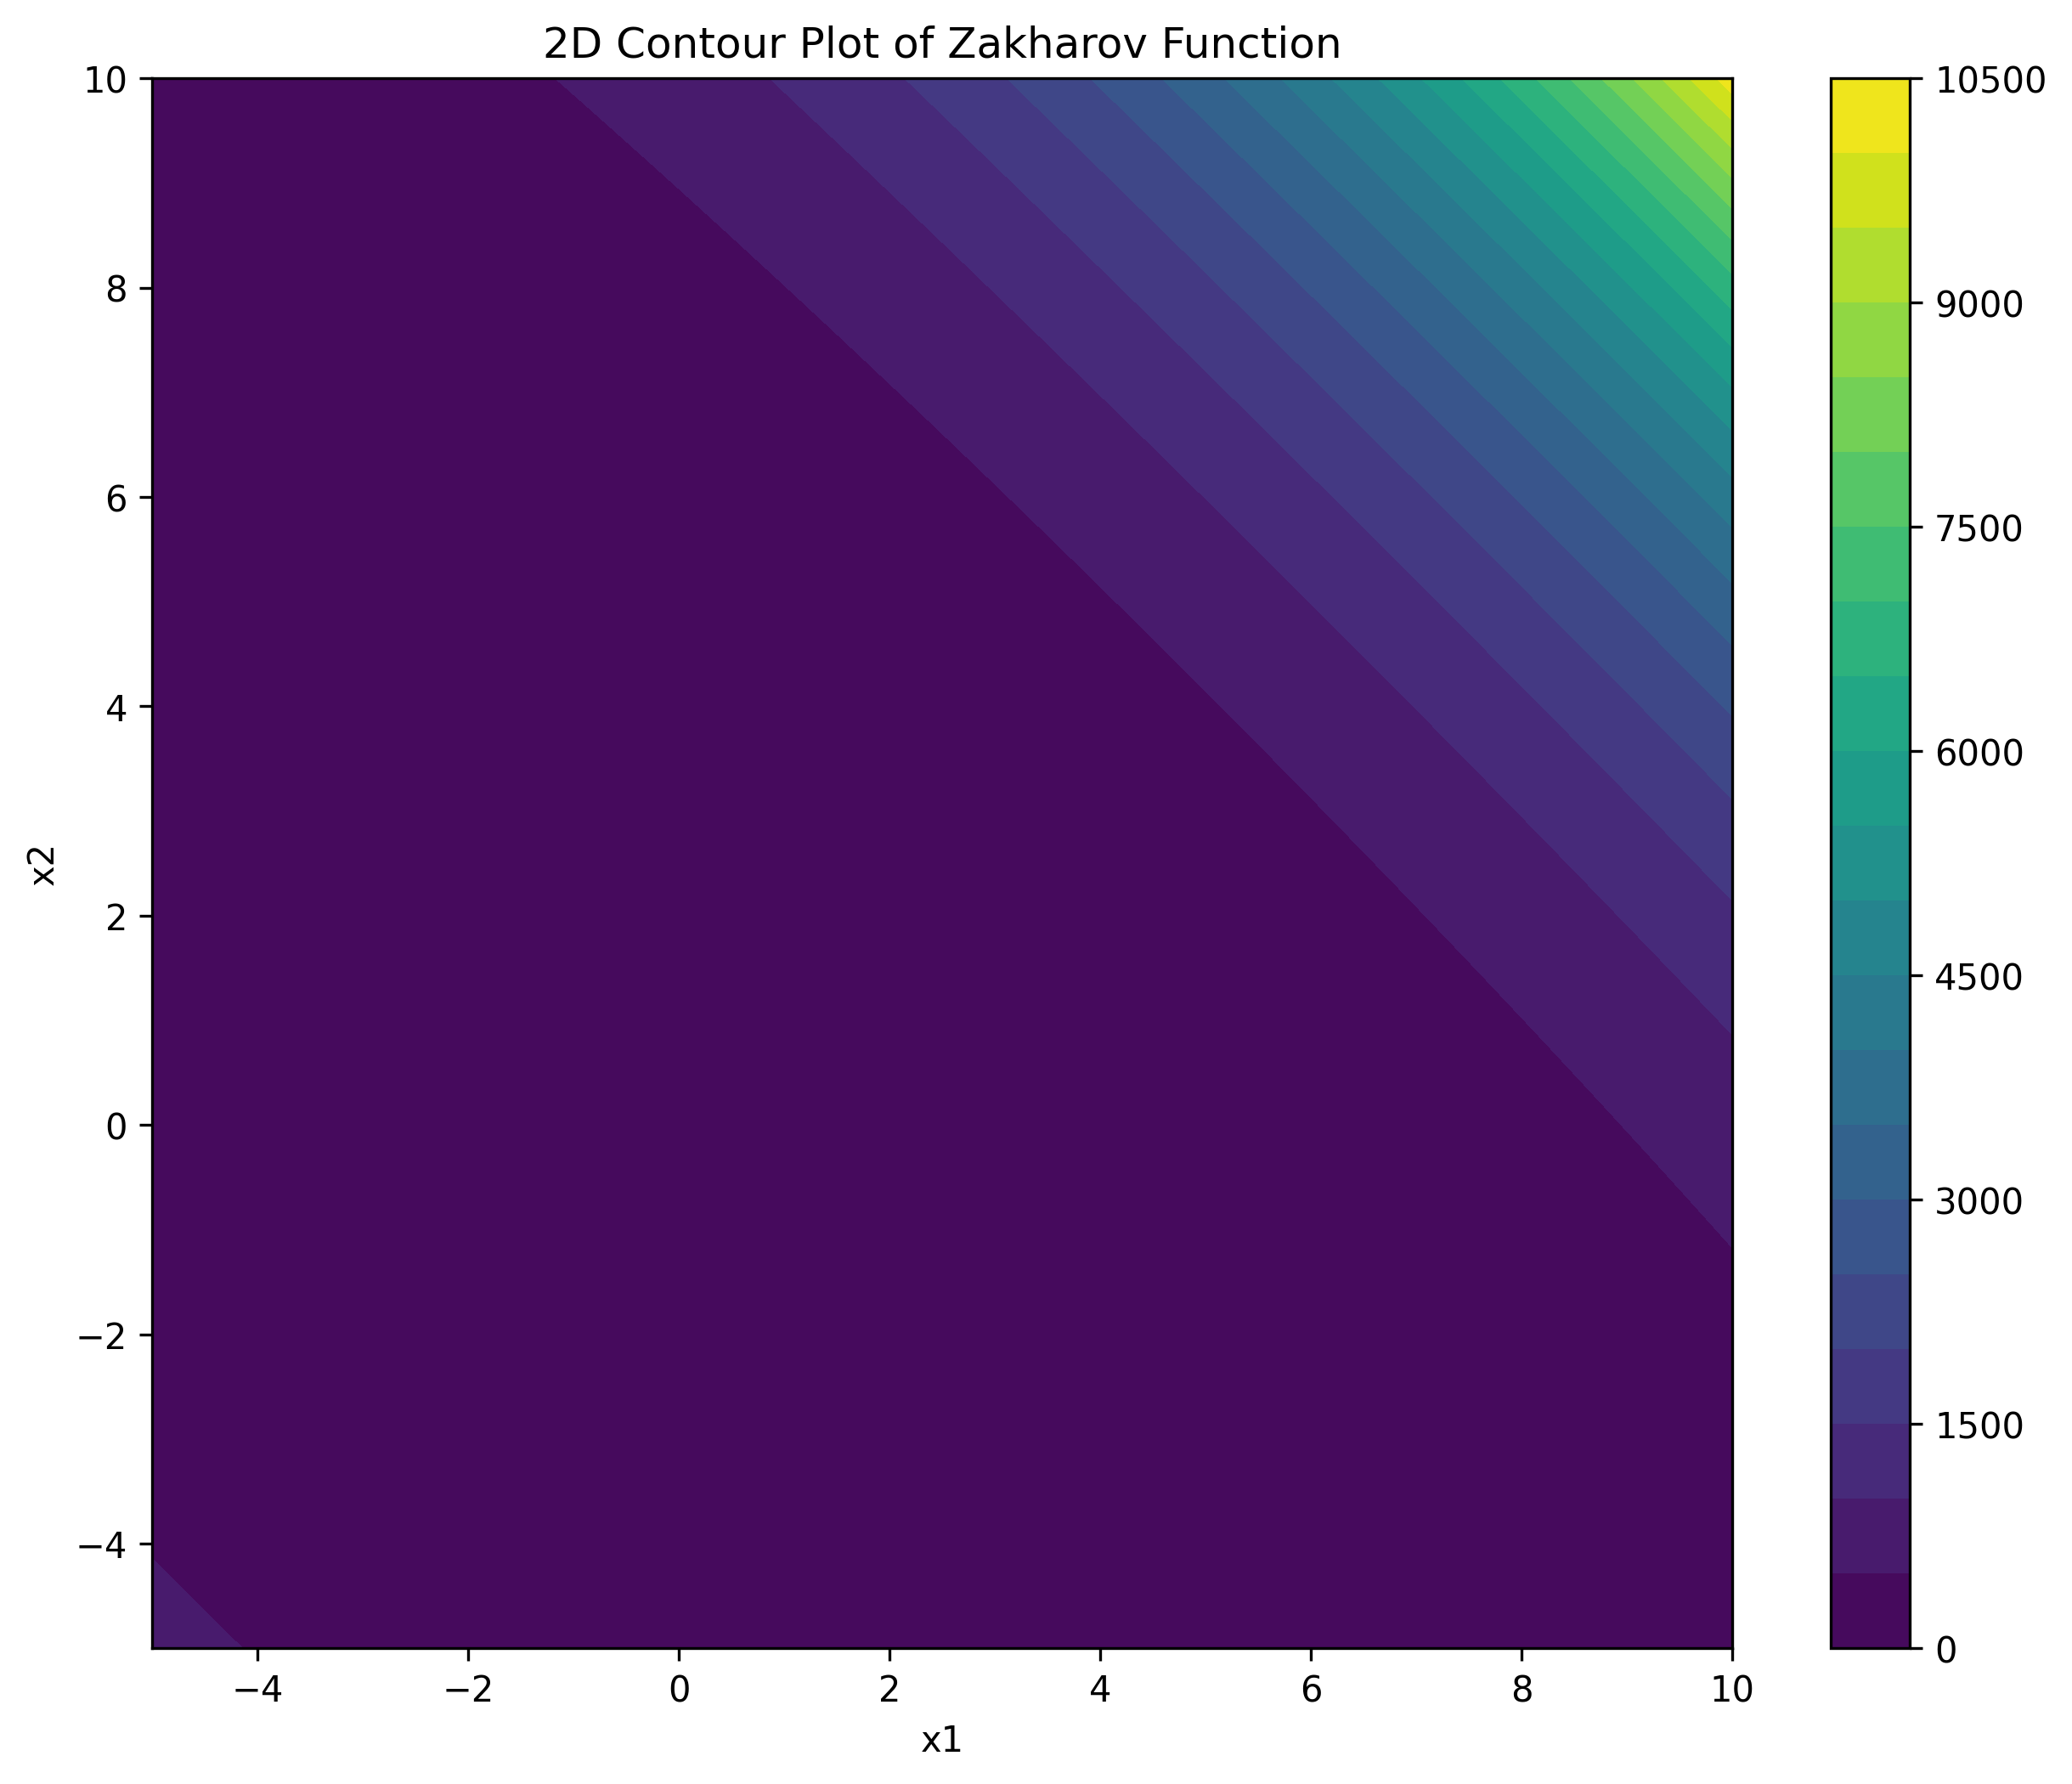
\includegraphics[width=\linewidth]{cec/zakharov_2d.png}
		\caption{Dimensi 2}
		\label{fig:zakharov-2d}
	\end{subfigure}
	\hfill
	\begin{subfigure}[b]{0.4\textwidth}
		\centering
		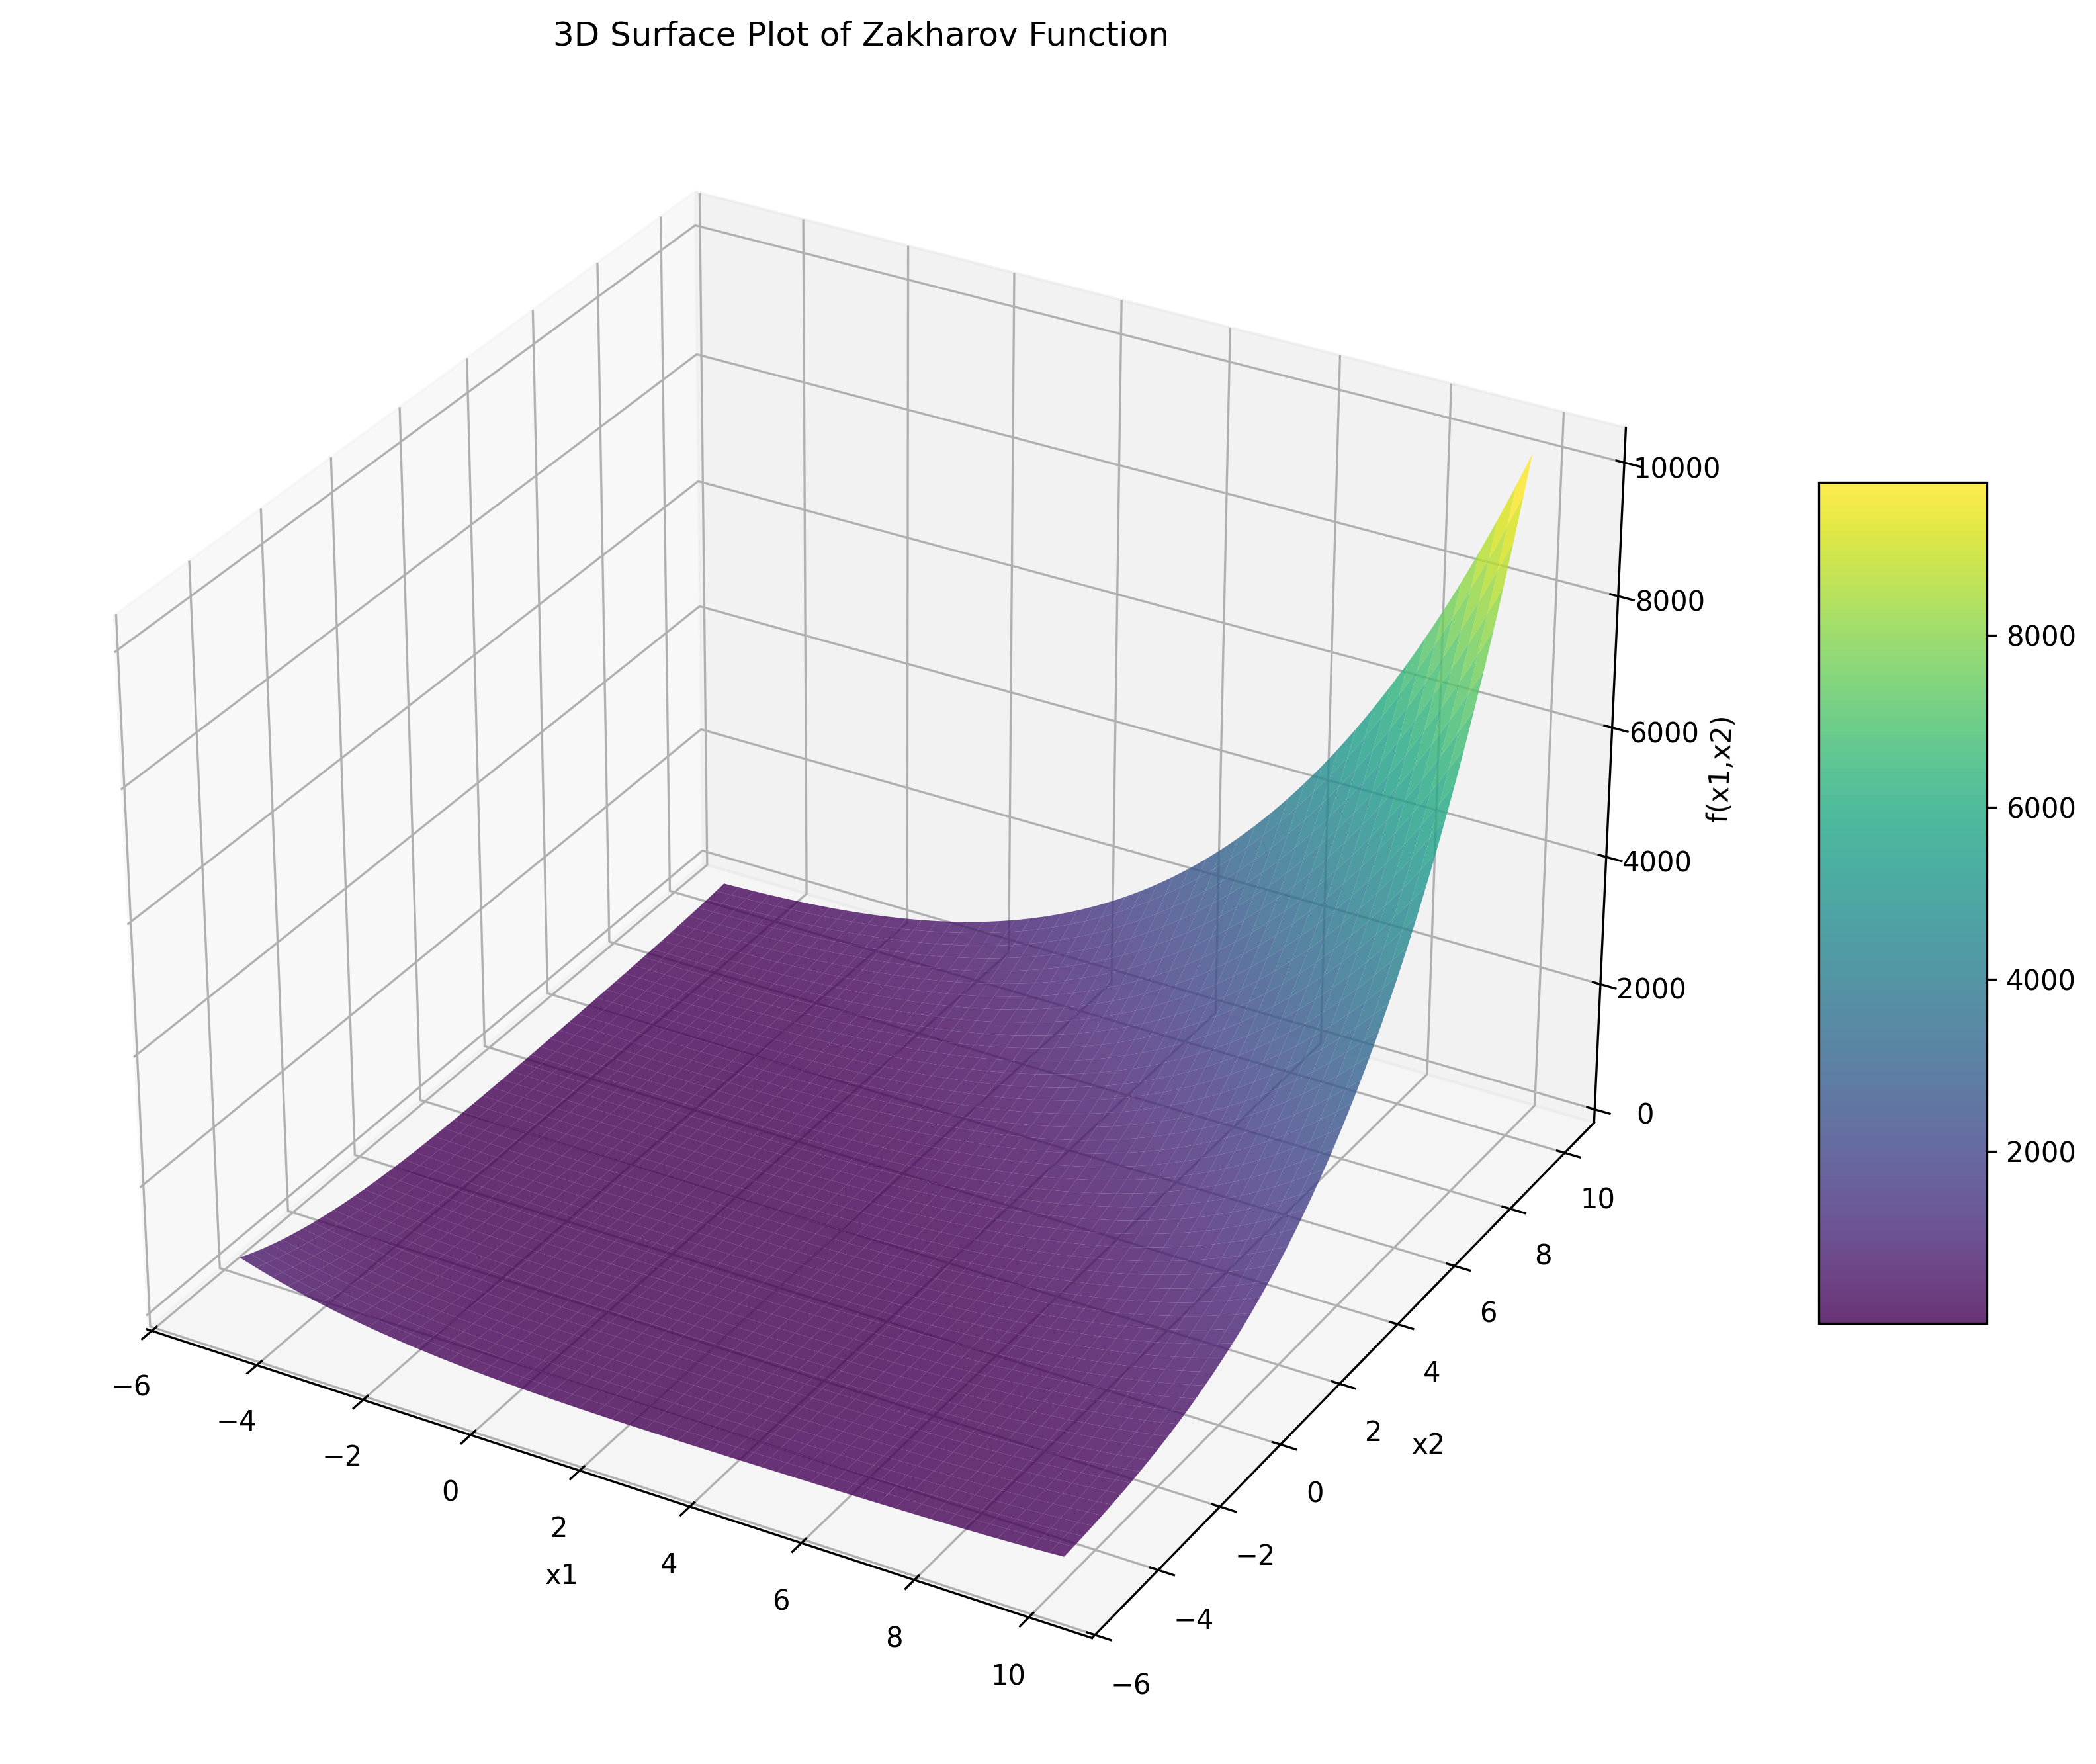
\includegraphics[width=\linewidth]{cec/zakharov_3d.png}
		\caption{Dimensi 3}
		\label{fig:zakharov-3d}
	\end{subfigure}
	\caption{Tampilan grafik fungsi Zakharov pada dimensi dua (\cref{fig:zakharov-2d}) dan tiga (\cref{fig:zakharov-3d})}
	\label{fig:zakharov}
\end{figure}
\begin{flalign*}
  f_{\text{Zakharov}}(\mathrm{x})=\sum_{i=1}^{D}z_i^2+\left(\sum_{i=1}^{D}0.5z_i \right)^2+\left(\sum_{i=1}^{D}0.5z_i \right)^4+f_{\text{bias}}&&
\end{flalign*}

\subsection{Fungsi COCO}
simbol dan definisi yang digunakan dalam fungsi COCO:\\
Lokasi optimal $\mathrm{x}^{\text{opt}}$ dan $f_{\text{opt}} = f(\mathrm{x}^{\text{opt}})$: Semua fungsi memiliki optimum global dalam $[-5, 5]^D$. Sebagian besar fungsi memiliki optimum global dalam $[-4, 4]^D$, dan untuk banyak di antaranya, $\mathrm{x}^{\text{opt}}$ diambil secara seragam dari kompak ini.\\
\noindent$\otimes$ menunjukkan perkalian per elemen antara dua vektor berdimensi $D$, $\otimes:R^D\times R^D\to R^D, (\mathrm{x},\mathrm{y})\mapsto \text{diag}(\mathrm{x})\times\mathrm{y}=(x_i\times y_i)_{i=1},\ldots,D$\\
$||\cdot||$ menunjukkan Euclidean norm, $||\mathrm{x}||^2=\sum_{i}x^2_i$\\
$\left[\cdot\right]$ menunjukkan nilai bilangan bulat terdekat\\
$\textbf{0}=(0,\ldots,0)^{\mathrm{T}}$ vektor yang semuanya bernilai 0\\
$\textbf{1}=(1,\ldots,1)^{\mathrm{T}}$ vektor yang semuanya bernilai 1\\
$\Lambda^{\alpha}$ adalah sebuah matriks diagonal berdimensi $D$ dengan elemen diagonal ke-$i$ sebagai $\lambda_{ii}=\alpha^{\frac{1}{2}\frac{i-1}{D-1}}$, untuk $i=1,\ldots,D$\\
$f_{\text{pen}}:\mathcal{R}^D\to \mathcal{R}, \mathrm{x}\mapsto\sum_{i=1}^{D}\max(0,\left|x_i\right|-5)^2$\\
$\textbf{1}\pm$ sebuah vektor berdimensi $D$ dengan entri bernilai $-1$ atau $1$ yang diambil secara independen dengan peluang yang sama\\
$\bf{Q, R}$ matriks ortogonal (matriks rotasi). Untuk satu fungsi dalam satu dimensi, realisasi yang berbeda untuk $Q$ dan $R$ masing-masing digunakan untuk setiap perwujudan fungsi tersebut. Ortogonal matriks dihasilkan dari entri berdistribusi normal standar melalui ortonormalisasi gram-schmidt. Kolom dan baris pada matriks ortogonal membentuk basis ortonormal.\\
$\bf{R}$ lihat $\bf{Q}$\\
$T_{\text{asy}}^{\beta}:\mathcal{R}^D\to \mathcal{R}^D,x_i\mapsto \begin{cases}
  x_i^{1+\beta\frac{i-1}{D-1}\sqrt{x_i}} & \text{jika } x_i > 0\\
  x_i & \text{selain itu}
\end{cases}, \text{untuk } i=1,\ldots,D$.\\
$T_{\text{osz}}:\mathcal{R}^n\to \mathcal{R}^n$, untuk sembarang bilangan bulat positif $n(n=1 \text{ dan } n=D \text{ yang digunakan berikut ini})$ peta kan \textit{element-wise}\\
\vspace*{-2.5em}
\[x\mapsto \sign(x) \exp(\hat{x}+0.049(\sin(c_1\hat{x})+\sin(c_2\hat{x})))\]
dengan $\hat{x}=\begin{cases}
  \log(\left|x\right|) & \text{jika } x > 0\\
  0 & \text{selain itu}
\end{cases}, \sign(x)=\begin{cases}
  -1 & \text{jika } x < 0\\
  0 & \text{jika } x = 0\\
  1 & \text{selain itu}
\end{cases},c_1=\begin{cases}
  10 & \text{jika } x > 0\\
  5.5 & \text{selain itu}
\end{cases}\text{ dan}\\ c_2=\begin{cases}
  7.9 & \text{jika } x > 0\\
  3.1 & \text{selain itu}
\end{cases}$.\\
$\mathrm{x}^{\text{opt}}$ vektor solusi optimal, sehingga $f(\mathrm{x}^{\text{opt}})$ adalah minimal.

\subsubsection{Attractive sector}
\noindent Properti:
fungsi dengan asimetris tingkat tinggi, di mana hanya terdapat satu \textit{hyperplane} bervolume sekitar $\frac{1}{2}^D$ yang memberikan nilai fungsi kecil.
\begin{packed_item}
  \item unimodal
\end{packed_item}
\begin{figure}[H]
	\centering
	\begin{subfigure}[b]{0.4\textwidth}
		\centering
		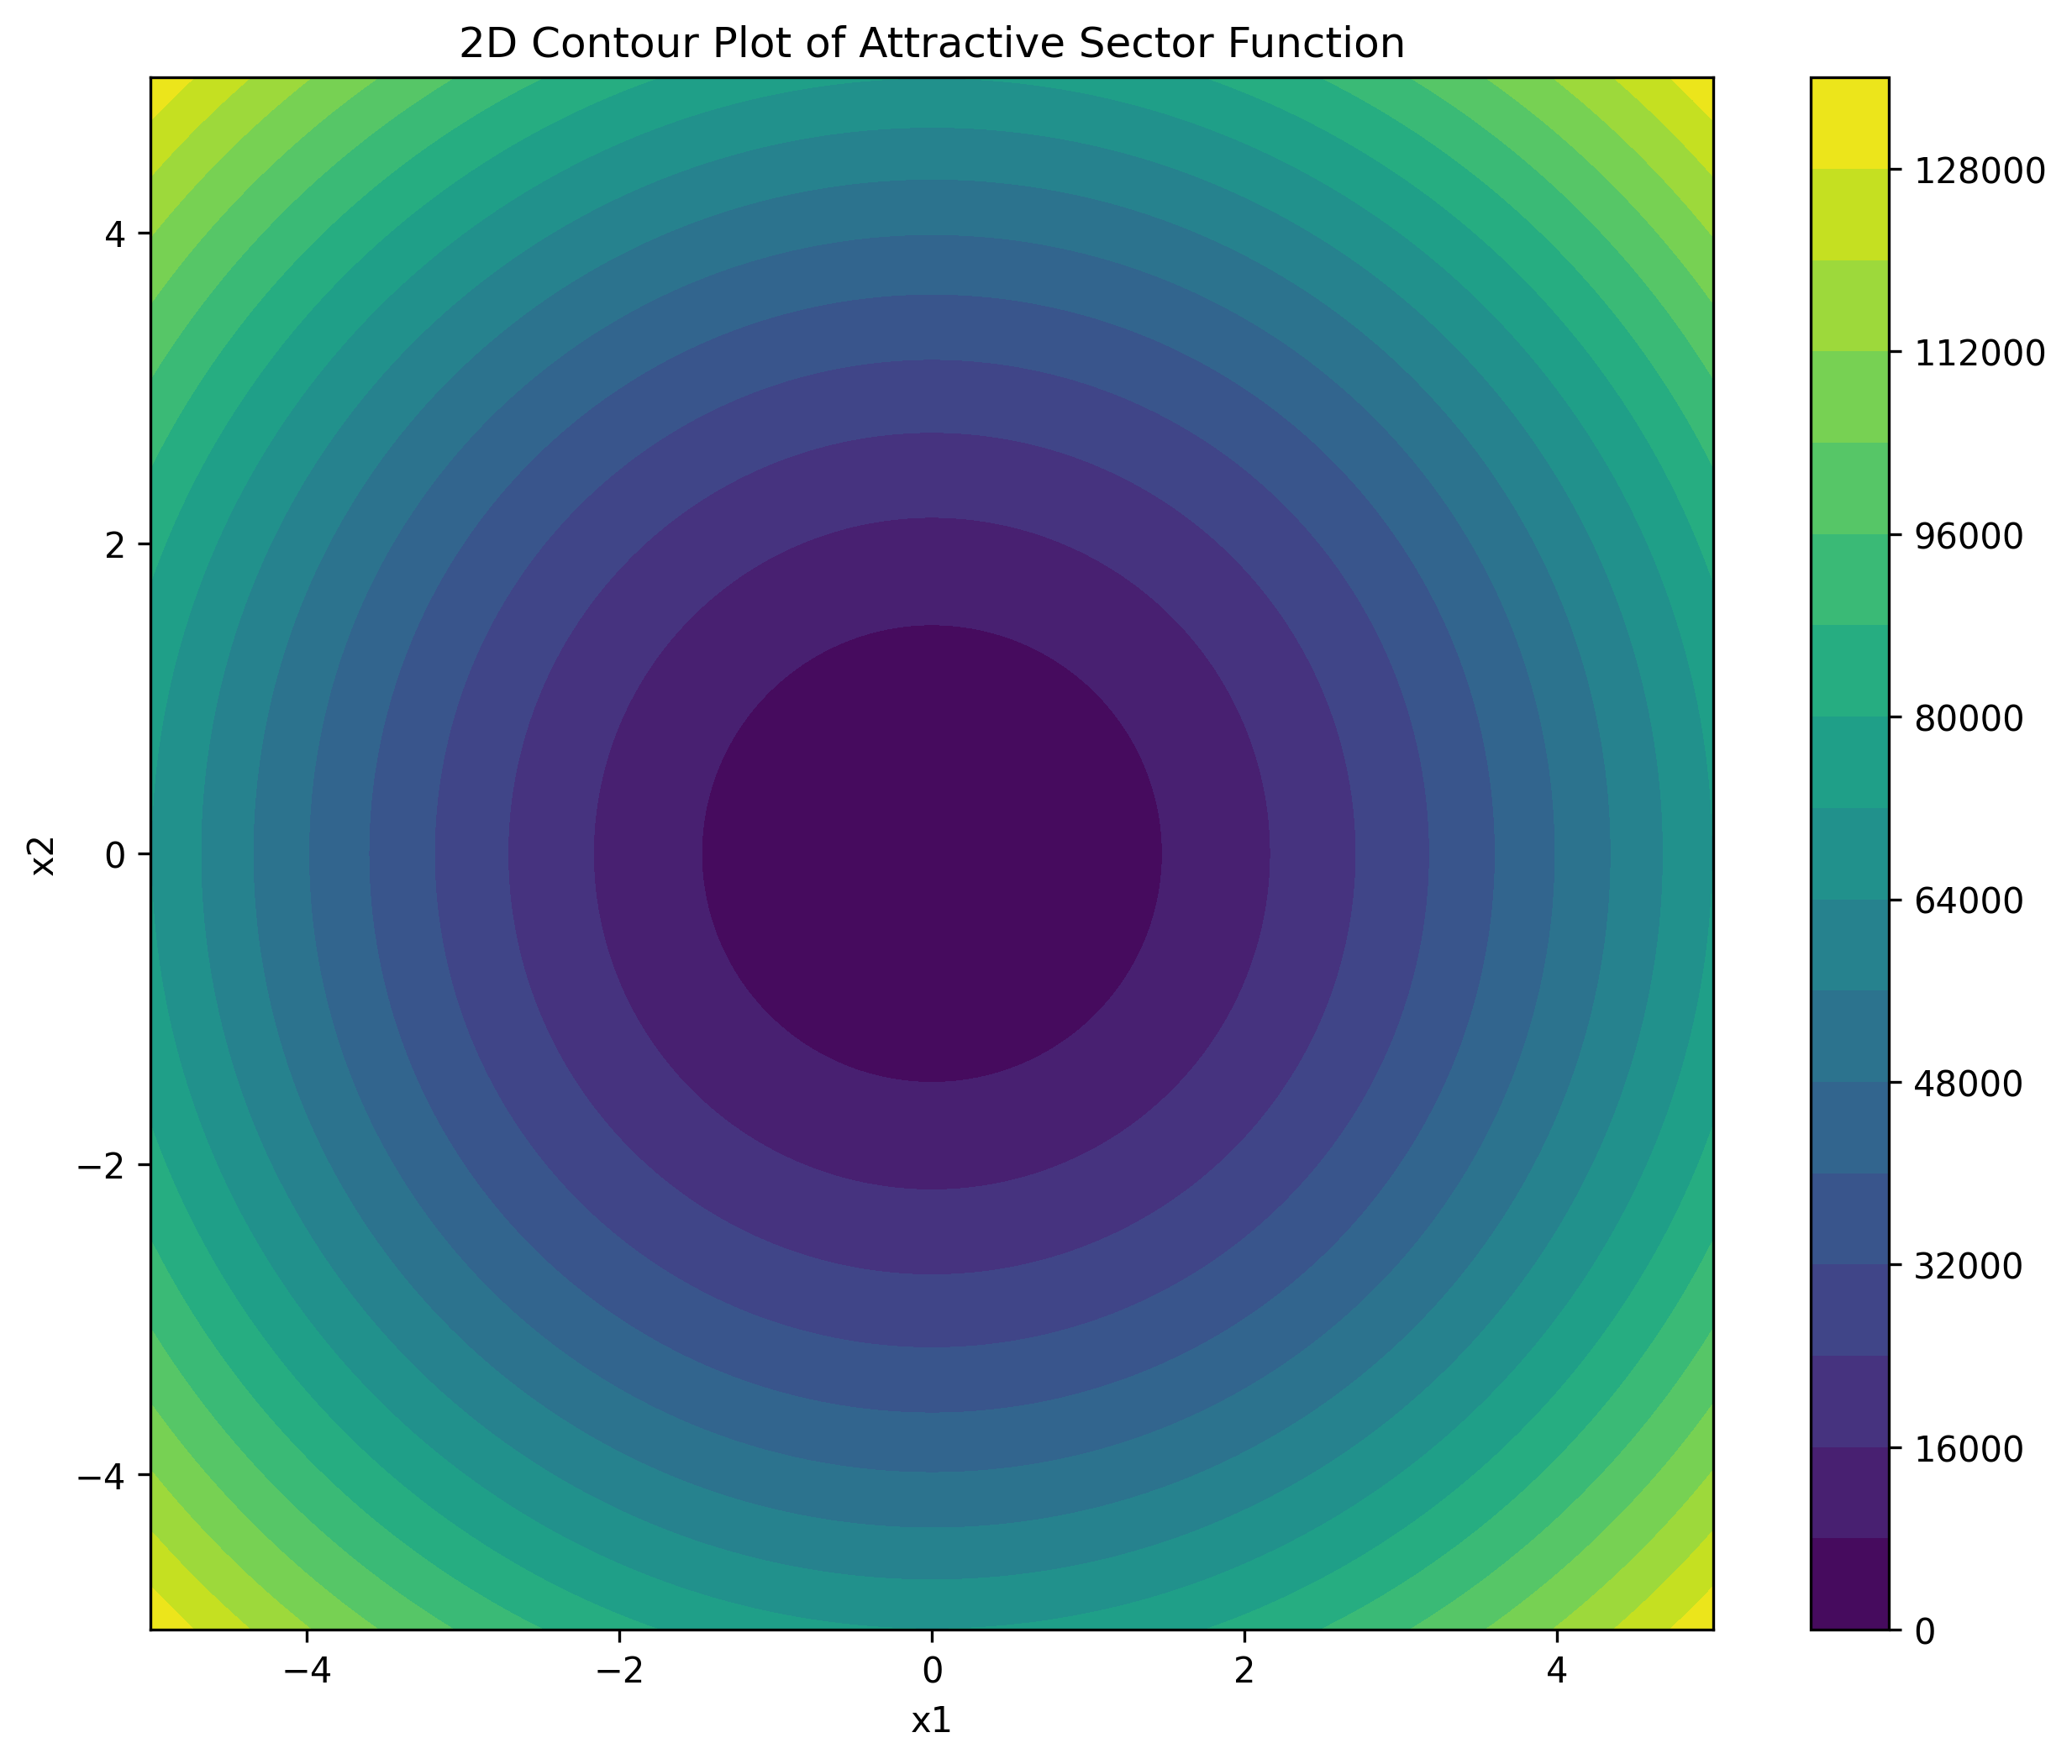
\includegraphics[width=\linewidth]{coco/attr_2d.png}
		\caption{Dimensi 2}
		\label{fig:attr-2d}
	\end{subfigure}
	\hfill
	\begin{subfigure}[b]{0.4\textwidth}
		\centering
		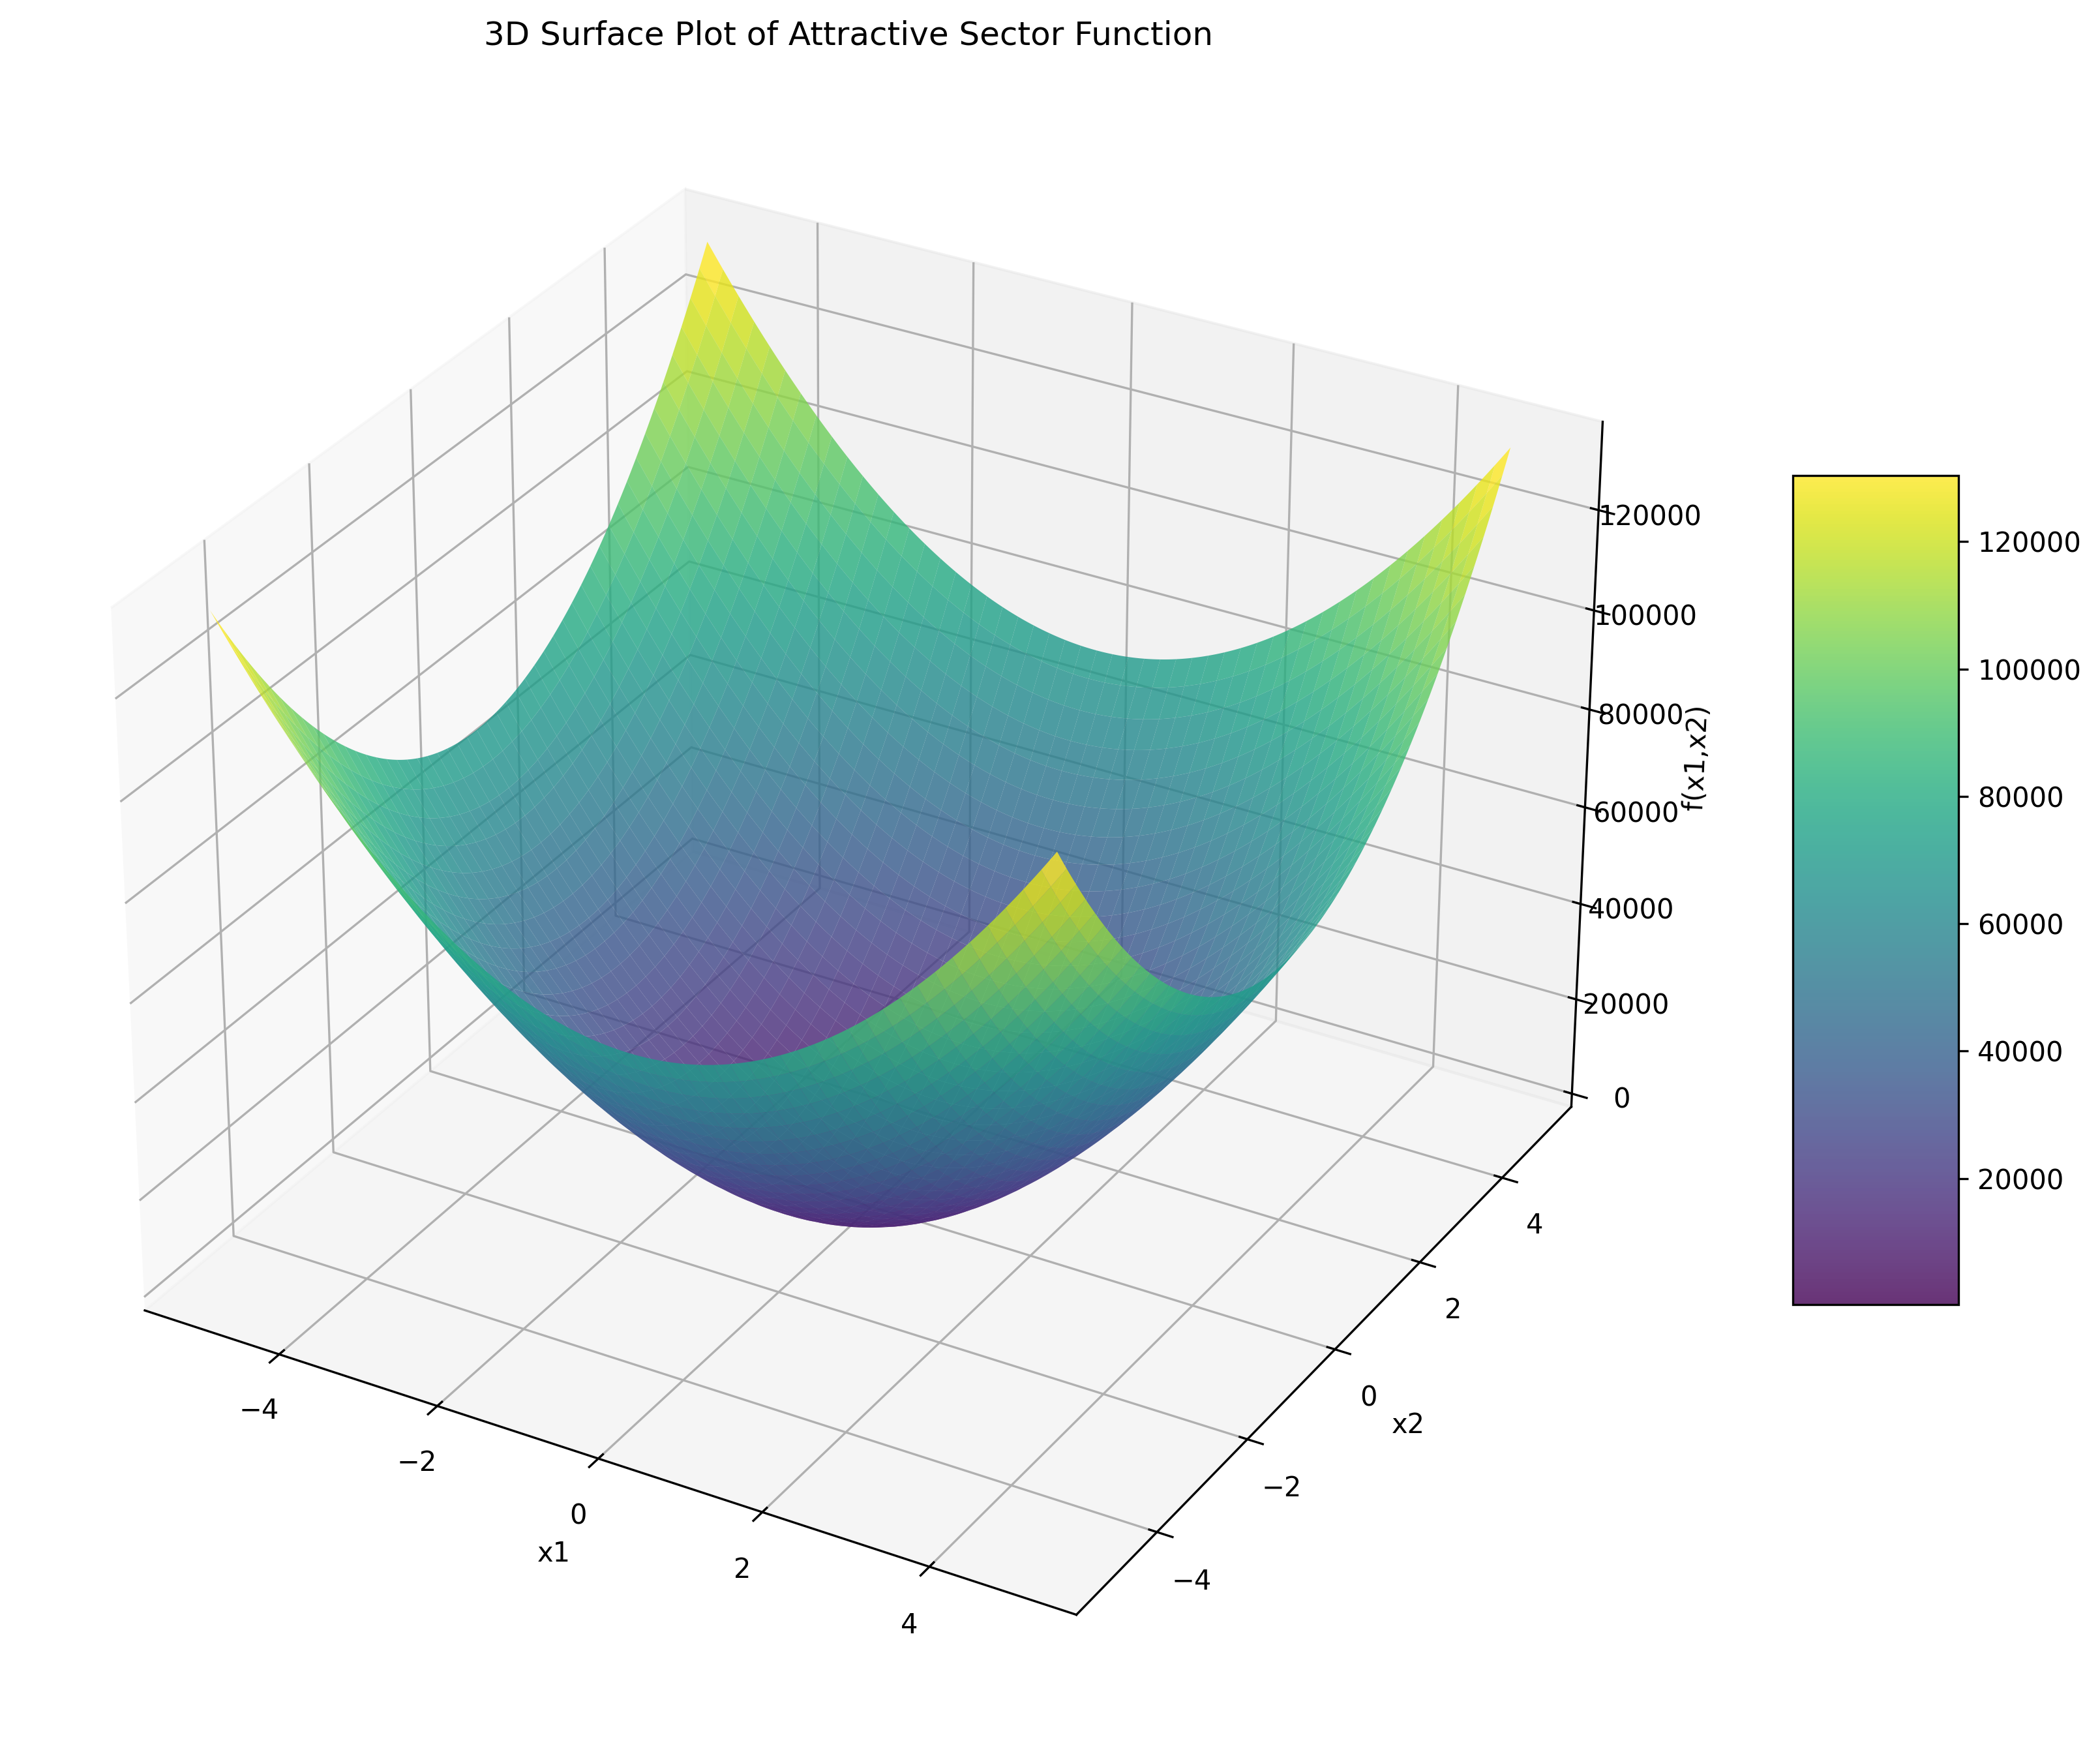
\includegraphics[width=\linewidth]{coco/attr_3d.png}
		\caption{Dimensi 3}
		\label{fig:attr-3d}
	\end{subfigure}
	\caption{Tampilan grafik fungsi Attractive sector pada dimensi dua (\cref{fig:attr-2d}) dan tiga (\cref{fig:attr-3d}) tanpa transformasi input}
	\label{fig:atrr}
\end{figure}
\vspace*{-2.5em}
\begin{flalign*}
  f_{\text{Attractive sector}}(\mathrm{x})=\mathrm{T}_{\text{osz}}(\sum_{i=1}^{D}(s_iz_i)^2)^{0.9}+f_{\text{opt}}&&\\
\end{flalign*}
\vspace*{-6.5em}
\begin{packed_item}
    \item $\mathrm{z}=Q\Lambda^{10}R(\mathrm{x}-\mathrm{x}^{\text{opt}})$
    \item $s_i\begin{cases}
      10^2 & \text{jika }z_i\times x_i^{\text{opt}}>0\\
      1 & \text{selain itu}
    \end{cases}$
\end{packed_item}

\subsubsection{Bent cigar}
\noindent Properti:
\begin{packed_item}
  \item unimodal
  \item struktur ketergantungan \textit{tri-band}, pada dimensi yang lebih tinggi fungsi ini memiliki optimal lokal dengan volume daya tarik sebesar 25\%
\end{packed_item}
\begin{figure}[H]
	\centering
	\begin{subfigure}[b]{0.4\textwidth}
		\centering
		\includegraphics[width=\linewidth]{coco/bent_cigar_2d.png}
		\caption{Dimensi 2}
		\label{fig:bent-cigar-coco-2d}
	\end{subfigure}
	\hfill
	\begin{subfigure}[b]{0.4\textwidth}
		\centering
		\includegraphics[width=\linewidth]{coco/bent_cigar_3d.png}
		\caption{Dimensi 3}
		\label{fig:bent-cigar-coco-3d}
	\end{subfigure}
	\caption{Tampilan grafik fungsi Bent cigar pada dimensi dua (\cref{fig:bent-cigar-coco-2d}) dan tiga (\cref{fig:bent-cigar-coco-3d}) tanpa transformasi input}
	\label{fig:bent_cigar_coco}
\end{figure}
\vspace*{-2.5em}
\begin{flalign*}
  f_{\text{Bent cigar}}(\mathrm{x})=\sum_{i=1}^{D-1}(100(z_i^2-z_{i+1})^2+(z_i-1)^2)+f_{\text{opt}}&&\\
\end{flalign*}
\vspace*{-6.5em}
\begin{packed_item}
    \item $\mathrm{z}=\max(1,\frac{\sqrt{D}}{8})(\mathrm{x}-\mathrm{x}^{\text{opt}})+1$
    \item $\mathrm{z}^{\text{opt}}=1$
\end{packed_item}

\subsubsection{Büche-Rastrigin}
\noindent Properti:
\begin{packed_item}
  \item sekitar $10^D$ optimum lokal, faktor pengkodisian sekitar 10, faktor \textit{skew} sekitar 10 di ruang ruang-$x$ dan 100 di ruang-$f$ 
\end{packed_item}
\begin{figure}[H]
	\centering
	\begin{subfigure}[b]{0.4\textwidth}
		\centering
		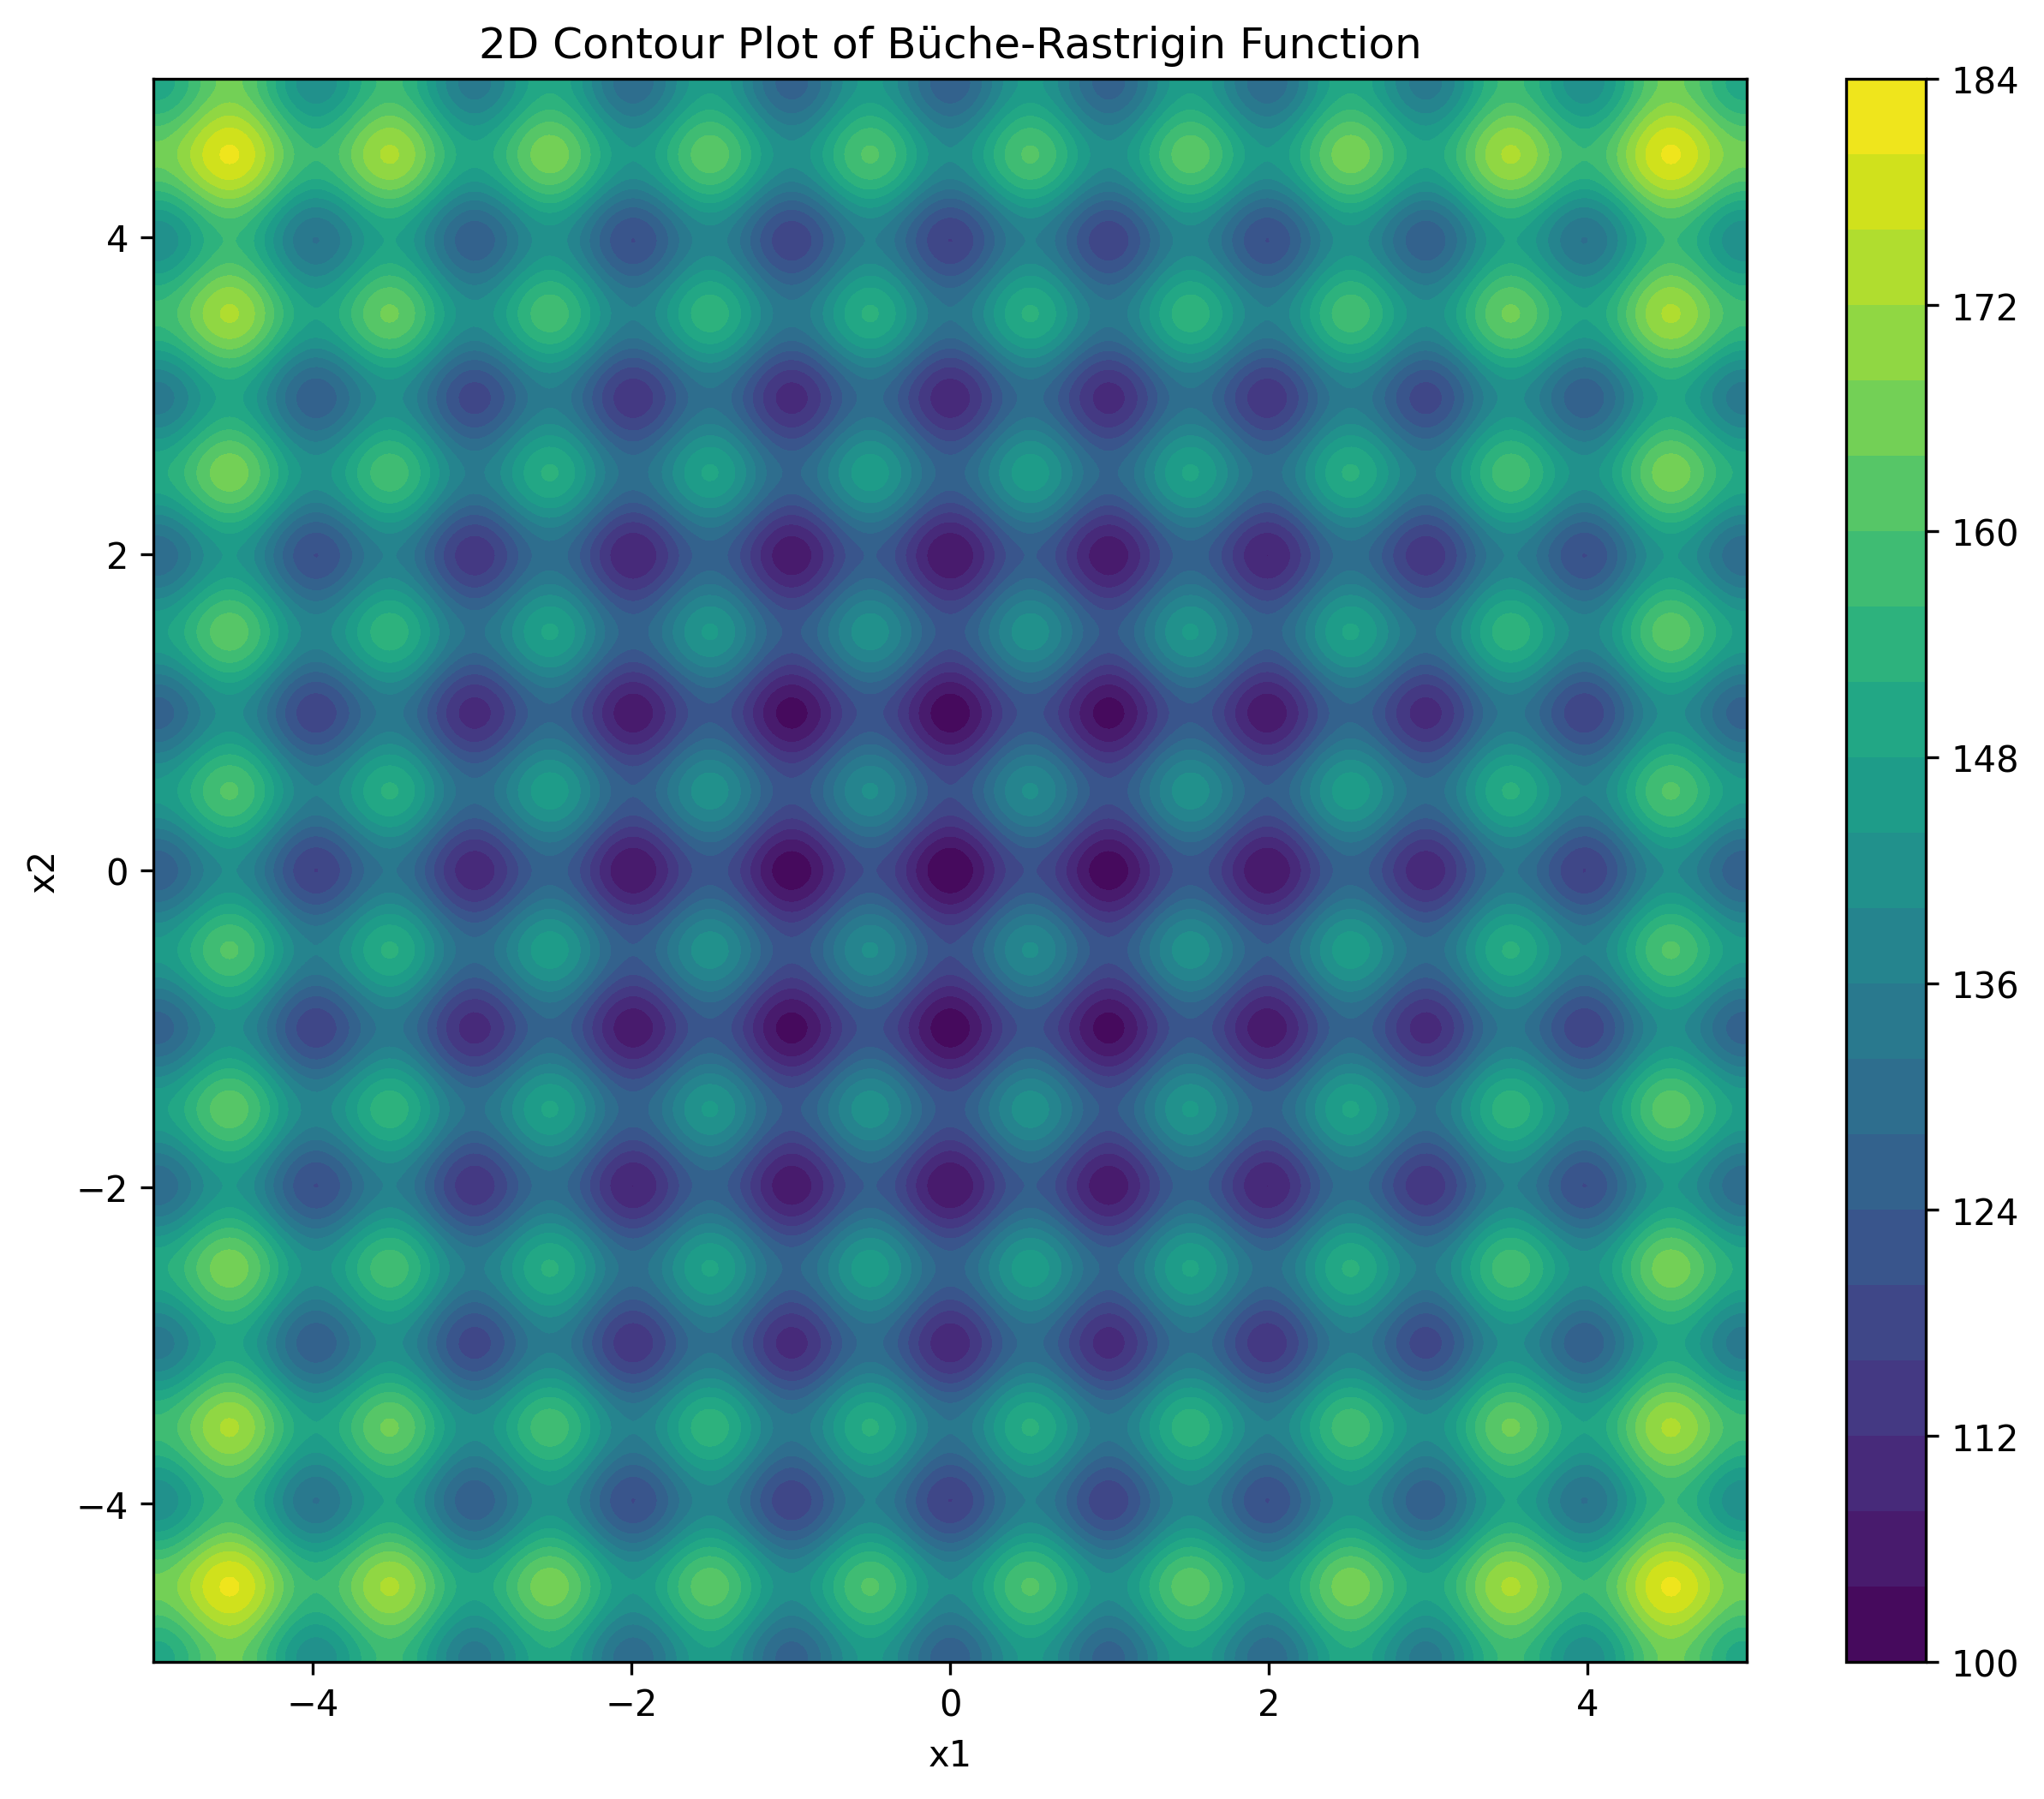
\includegraphics[width=\linewidth]{coco/buche_rastrigin_2d.png}
		\caption{Dimensi 2}
		\label{fig:buche-rastrigin-2d}
	\end{subfigure}
	\hfill
	\begin{subfigure}[b]{0.4\textwidth}
		\centering
		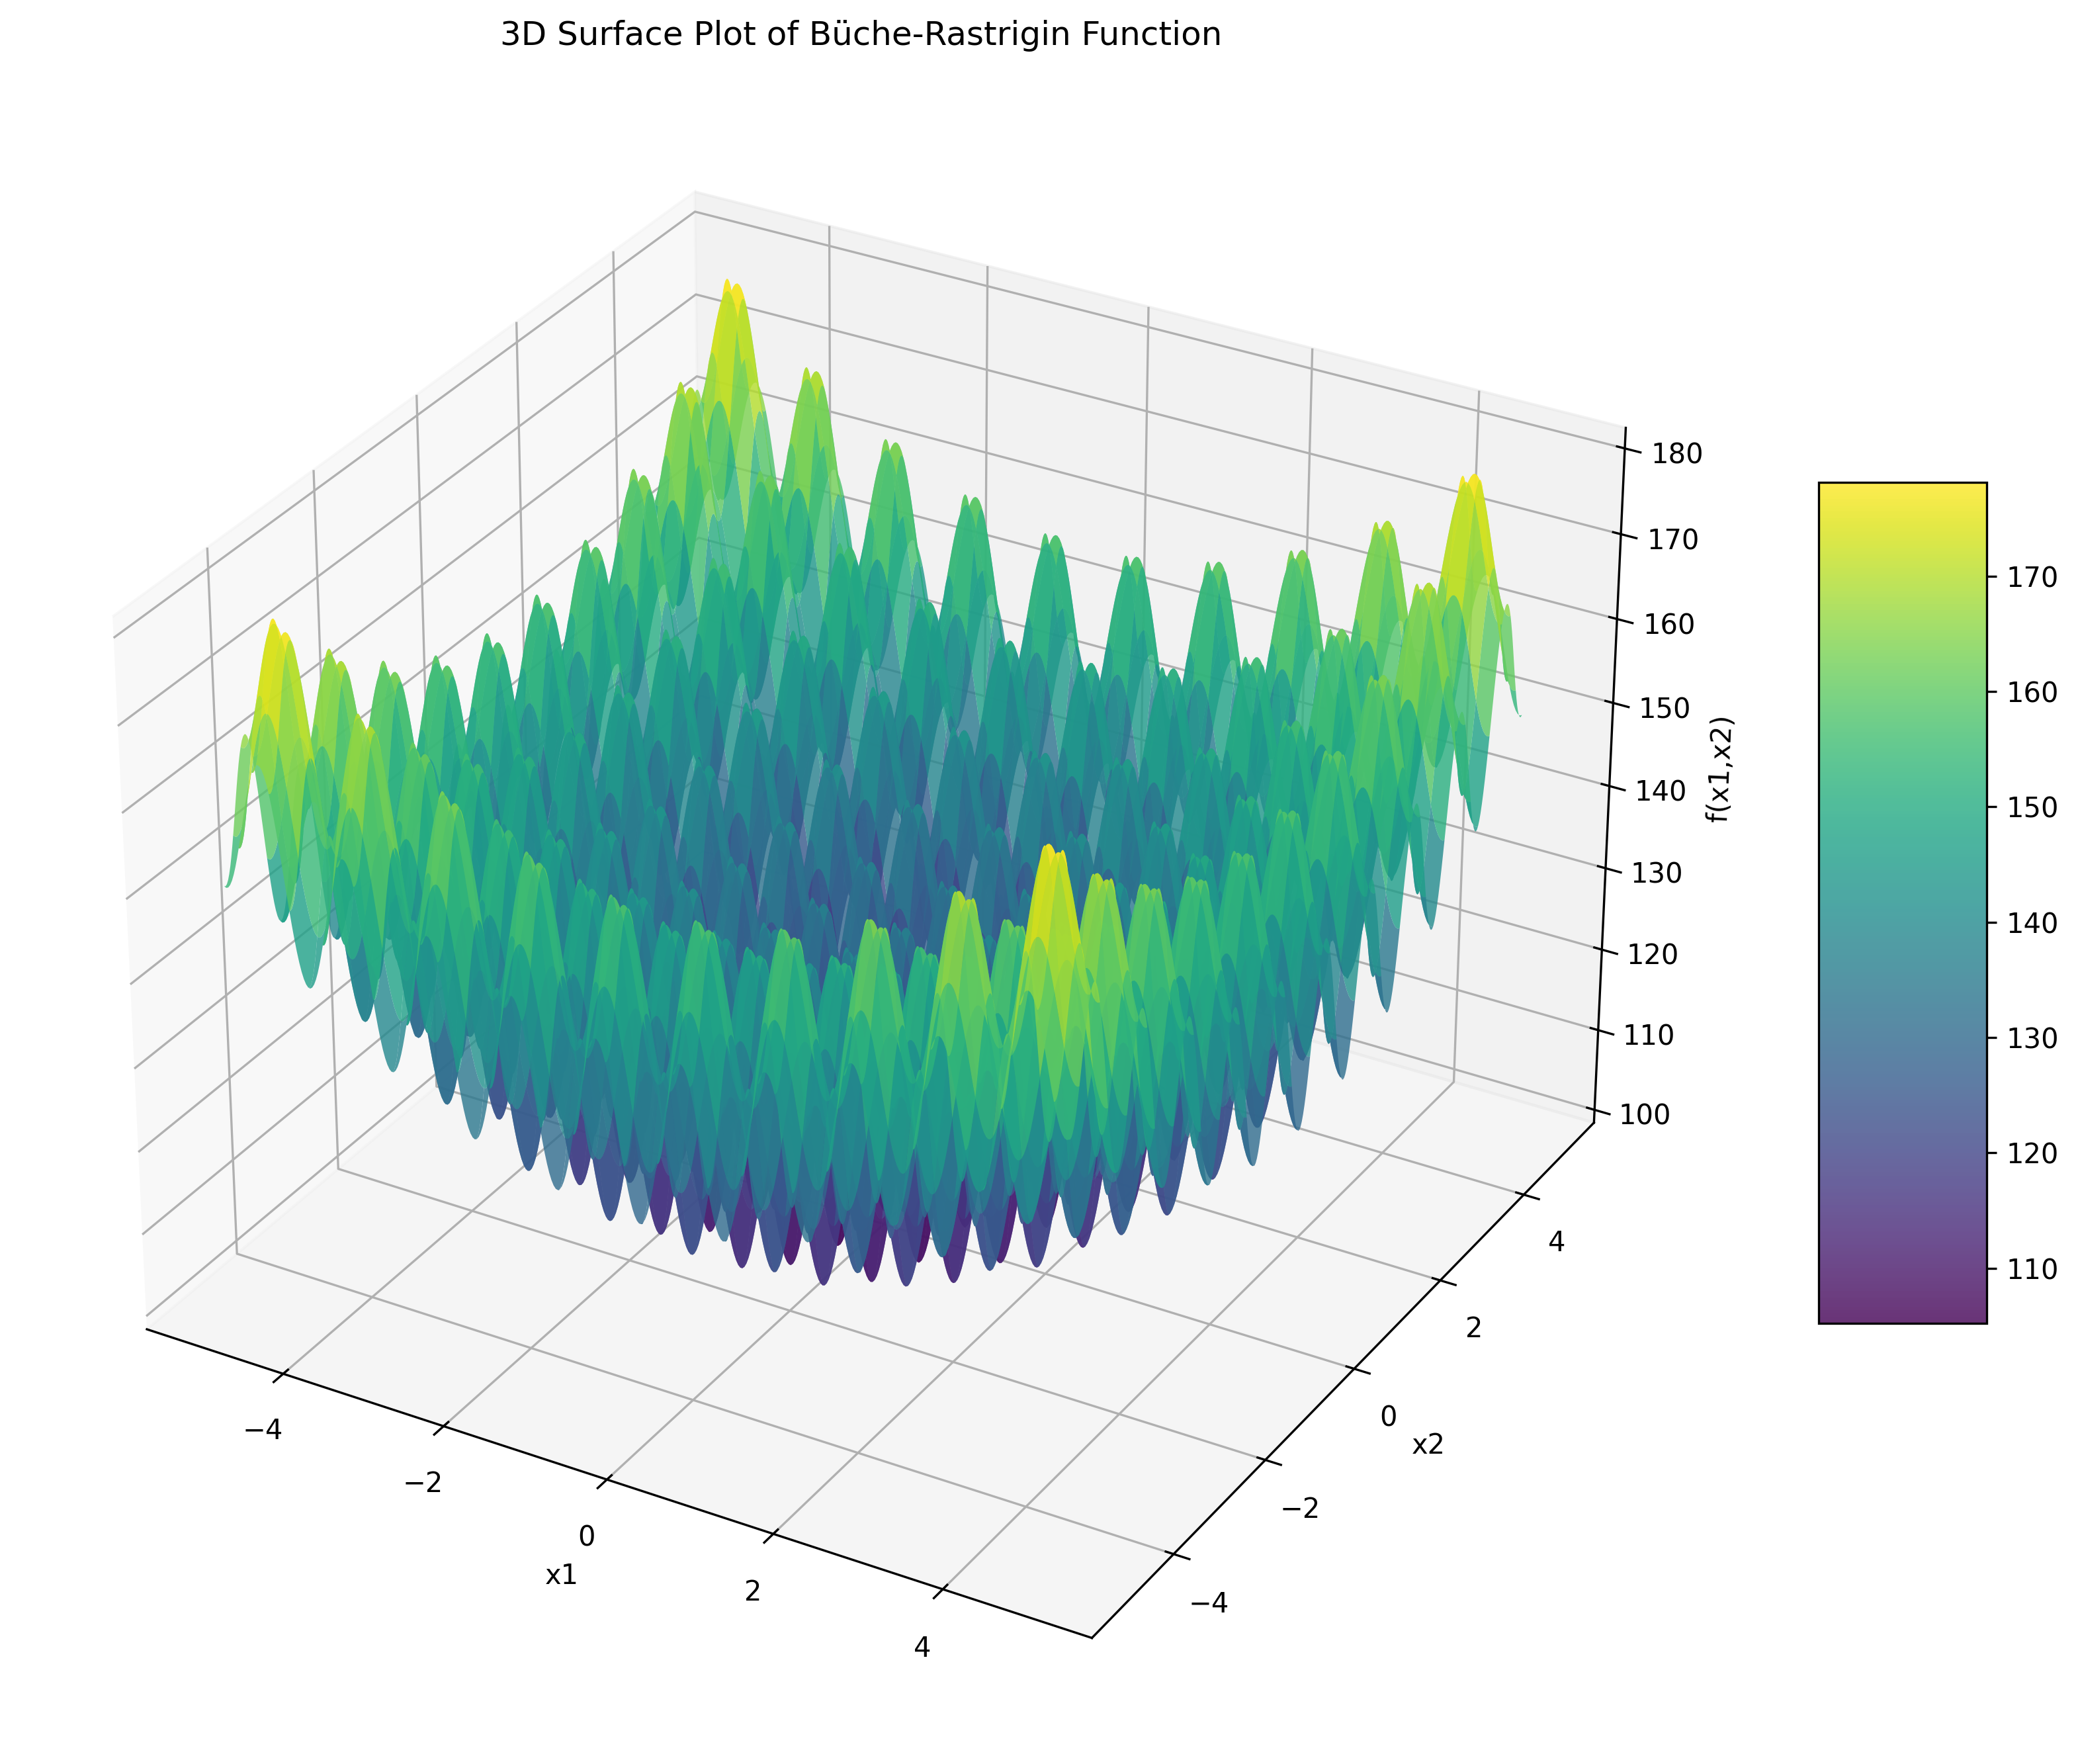
\includegraphics[width=\linewidth]{coco/buche_rastrigin_3d.png}
		\caption{Dimensi 3}
		\label{fig:buche-rastrigin-3d}
	\end{subfigure}
	\caption{Tampilan grafik fungsi Büche-Rastrigin pada dimensi dua (\cref{fig:buche-rastrigin-2d}) dan tiga (\cref{fig:buche-rastrigin-3d}) tanpa transformasi input}
	\label{fig:buche_rastrigin}
\end{figure}
\vspace*{-2.5em}
\begin{flalign*}
  f_{\text{Büche-Rastrigin}}(\mathrm{x})=10(D-\sum_{i=1}^{D}\cos(2\pi z_i))+\sum_{i=1}^{D}z_i^2+100f_{\text{pen}}(\mathrm{x})+f_{\text{opt}}&&\\
\end{flalign*}
\vspace*{-6.5em}
\begin{packed_item}
    \item $z_i=s_iT_{\text{osz}}(\mathrm{x}-\mathrm{x}^{\text{opt}})$ untuk $i=1,\ldots,D$
    \item $s_i=\begin{cases}
      10\times 10^{\frac{1}{2}\frac{i-1}{D-1}} & \text{jika }z_i > 0 \text{ dan } i=1,3,5,\ldots\\
      10^{\frac{1}{2}\frac{i-1}{D-1}} & \text{selain itu}
    \end{cases} \text{ untuk }i=1,\ldots,D$
\end{packed_item}

\subsubsection{Composite griewank-rosenbrock function F8F2}
\noindent Properti:
menyerupai fungsi rosenbrock dengan dalam sifat yang sangat multimodal
\begin{figure}[H]
	\centering
	\begin{subfigure}[b]{0.4\textwidth}
		\centering
		\includegraphics[width=\linewidth]{coco/griewank_rosenbrock_2d.png}
		\caption{Dimensi 2}
		\label{fig:griewank-rosenbrock-2d}
	\end{subfigure}
	\hfill
	\begin{subfigure}[b]{0.4\textwidth}
		\centering
		\includegraphics[width=\linewidth]{coco/griewank_rosenbrock_3d.png}
		\caption{Dimensi 3}
		\label{fig:griewank-rosenbrock-3d}
	\end{subfigure}
	\caption{Tampilan grafik fungsi Composite griewank-rosenbrock function F8F2 pada dimensi dua (\cref{fig:griewank-rosenbrock-2d}) dan tiga (\cref{fig:griewank-rosenbrock-3d}) tanpa transformasi input}
	\label{fig:griewank_rosenbrock}
\end{figure}
\vspace*{-2.5em}
\begin{flalign*}
  f_{\text{Büche-Rastrigin}}(\mathrm{x})=\frac{10}{D-1}\sum_{i=1}^{D-1}(\frac{s_i}{4000}-\cos(s_i))+10+f_{\text{opt}}&&\\
\end{flalign*}
\vspace*{-6.5em}
\begin{packed_item}
    \item $\mathrm{z}=\max(1,\frac{\sqrt{D}}{8})R\mathrm{x}+0.5$
    \item $s_i=100(z_i^2-z_{i+1})^2+(z_i-1)^2$ untuk $i=1,\ldots,D$
    \item $\mathrm{z}^{\text{opt}}=1$
\end{packed_item}

\subsubsection{Different power}
\noindent Properti:
karena perbedaan exponen, sensitivitas variabel $z_i$ menjadi semakin berbeda ketika mendekati titik optimum.
\begin{figure}[H]
	\centering
	\begin{subfigure}[b]{0.4\textwidth}
		\centering
		\includegraphics[width=\linewidth]{coco/different_power_2d.png}
		\caption{Dimensi 2}
		\label{fig:dp_2d}
	\end{subfigure}
	\hfill
	\begin{subfigure}[b]{0.4\textwidth}
		\centering
		\includegraphics[width=\linewidth]{coco/different_power_3d.png}
		\caption{Dimensi 3}
		\label{fig:dp_3d}
	\end{subfigure}
	\caption{Tampilan grafik fungsi Different power pada dimensi dua (\cref{fig:dp_2d}) dan tiga (\cref{fig:dp_3d}) tanpa transformasi input}
	\label{fig:different_power_coco}
\end{figure}
\vspace*{-2.5em}
\begin{flalign*}
  f_{\text{Different power}}(\mathrm{x})=\sqrt{\sum_{i=1}^{D}|z_i|^{2+4\frac{i-1}{D-1}}}+f_{\text{opt}}&&\\
\end{flalign*}
\vspace*{-6.5em}
\begin{packed_item}
    \item $\mathrm{z}=R(\mathrm{x}-\mathrm{x}^{\text{opt}})$
\end{packed_item}

\subsubsection{Discus}
\noindent Properti:
Fungsi yang secara global kuadratik namun memiliki penyimpangan lokal. Terdapat satu arah tertentu dalam ruang pencarian yang kepekaannya seribu kali lipat lebih besar daripada arah lainnya.
\begin{packed_item}
  \item nilai pengkondisian sekitar $10^6$
\end{packed_item}
\begin{figure}[H]
	\centering
	\begin{subfigure}[b]{0.4\textwidth}
		\centering
		\includegraphics[width=\linewidth]{coco/discus_2d.png}
		\caption{Dimensi 2}
		\label{fig:discus_coco_2d}
	\end{subfigure}
	\hfill
	\begin{subfigure}[b]{0.4\textwidth}
		\centering
		\includegraphics[width=\linewidth]{coco/discus_3d.png}
		\caption{Dimensi 3}
		\label{fig:discus_coco_3d}
	\end{subfigure}
	\caption{Tampilan grafik fungsi Discus pada dimensi dua (\cref{fig:discus_coco_2d}) dan tiga (\cref{fig:discus_coco_3d}) tanpa transformasi input}
	\label{fig:discus_coco}
\end{figure}
\vspace*{-2.5em}
\begin{flalign*}
  f_{\text{Discus}}(\mathrm{x})=10^6z_1^2+\sum_{i=2}^{D}z_i^2+f_{\text{opt}}&&\\
\end{flalign*}
\vspace*{-6.5em}
\begin{packed_item}
    \item $\mathrm{z}=T_{\text{osz}}(R(\mathrm{x}-\mathrm{x}^{\text{opt}}))$
\end{packed_item}

\subsubsection{Ellipsoidal}
\noindent Properti:
(Separable) Fungsi kuadratik global dengan pengkondisian buruk dan ketidakteraturan lokal yang halus.\\
(With high conditioning and unimodal) Fungsi kuadratik global berkondisi buruk dengan ketidakteraturan lokal halus, merupakan pasangan non-separable dari fungsi f2.
\begin{packed_item}
  \item unimodal
  \item nilai pengkondisian sekitar $10^6$
\end{packed_item}
\begin{figure}[H]
	\centering
	\begin{subfigure}[b]{0.4\textwidth}
		\centering
		\includegraphics[width=\linewidth]{coco/ellipsoidal_2d.png}
		\caption{Dimensi 2}
		\label{fig:ellipsoidal_2d}
	\end{subfigure}
	\hfill
	\begin{subfigure}[b]{0.4\textwidth}
		\centering
		\includegraphics[width=\linewidth]{coco/ellipsoidal_3d.png}
		\caption{Dimensi 3}
		\label{fig:ellipsoidal_3d}
	\end{subfigure}
	\caption{Tampilan grafik fungsi Ellipsoidal pada dimensi dua (\cref{fig:ellipsoidal_2d}) dan tiga (\cref{fig:ellipsoidal_3d}) tanpa transformasi input}
	\label{fig:ellipsoidal}
\end{figure}
\vspace*{-2.5em}
\begin{flalign*}
  f_{\text{Ellipsoidal}}(\mathrm{x})=\sum_{i=2}^{D}10^{6\frac{i-1}{D-1}}+f_{\text{opt}}&&\\
\end{flalign*}
\vspace*{-6.5em}
\begin{packed_item}
    \item $\mathrm{z}=T_{\text{osz}}(\mathrm{x}-\mathrm{x}^{\text{opt}})\text{ (separable)}$\\
    \item $\mathrm{z}=T_{\text{osz}}(R(\mathrm{x}-\mathrm{x}^{\text{opt}}))\text{ (with high conditioning and unimodal)}$
\end{packed_item}

\subsubsection{Katsuura}
\noindent Properti:
Fungsi dengan tingkat kekasaran dan repetisi tinggi yang memiliki lebih dari $10^D$ optimum global, dikembangkan berdasarkan konsep dalam \citep{Katsuura:1991:CND}
\begin{figure}[H]
	\centering
	\begin{subfigure}[b]{0.4\textwidth}
		\centering
		\includegraphics[width=\linewidth]{coco/katsuura_2d.png}
		\caption{Dimensi 2}
		\label{fig:katsuura_coco_2d}
	\end{subfigure}
	\hfill
	\begin{subfigure}[b]{0.4\textwidth}
		\centering
		\includegraphics[width=\linewidth]{coco/katsuura_3d.png}
		\caption{Dimensi 3}
		\label{fig:katsuura_coco_3d}
	\end{subfigure}
	\caption{Tampilan grafik fungsi Katsuura pada dimensi dua (\cref{fig:katsuura_coco_2d}) dan tiga (\cref{fig:katsuura_coco_3d}) tanpa transformasi input}
	\label{fig:katsuura_coco}
\end{figure}
\vspace*{-2.5em}
\begin{flalign*}
  f_{\text{Sphere}}(\mathrm{x})=\frac{10}{D}\prod_{i=1}^{D}(1+i\sum_{j=1}^{32}\frac{|2^jz_i-[2^jz_i]|}{2^j})^{\frac{10}{D^{1.2}}}+f_{\text{opt}}&&\\
\end{flalign*}
\vspace*{-6.5em}
\begin{packed_item}
    \item $\mathrm{z}=Q\Lambda^{100}R(\mathrm{x}-\mathrm{x}^{\text{opt}})$
\end{packed_item}

\subsubsection{Linear slope}
\noindent Properti:
Fungsi linear sepenuhnya yang bertujuan menguji apakah proses pencarian mampu keluar dari \textit{convex hull} solusi awal dan mencapai batas domain.
\begin{packed_item}
  \item $\mathrm{x}^{\text{opt}}$ berada di batas domain.
\end{packed_item}
\begin{figure}[H]
	\centering
	\begin{subfigure}[b]{0.4\textwidth}
		\centering
		\includegraphics[width=\linewidth]{coco/linear_slope_2d.png}
		\caption{Dimensi 2}
		\label{fig:linear_slope_2d}
	\end{subfigure}
	\hfill
	\begin{subfigure}[b]{0.4\textwidth}
		\centering
		\includegraphics[width=\linewidth]{coco/linear_slope_3d.png}
		\caption{Dimensi 3}
		\label{fig:linear_slope_3d}
	\end{subfigure}
	\caption{Tampilan grafik fungsi Linear slope pada dimensi dua (\cref{fig:linear_slope_2d}) dan tiga (\cref{fig:linear_slope_3d}) tanpa transformasi input}
	\label{fig:linear_slope}
\end{figure}
\vspace*{-2.5em}
\begin{flalign*}
  f_{\text{Sphere}}(\mathrm{x})=\sum_{i=1}^{D}5|s_i|-s_iz_i+f_{\text{opt}}&&\\
\end{flalign*}
\vspace*{-6.5em}
\begin{packed_item}
    \item $z_i=x_i$ jika $x_i^{\text{opt}}x_i < 5^2$ dan selain itu $z_i=x_i^{\text{opt}}$, untuk $i=1,\ldots,D$. Dengan kata lain, apabila $x_i$ melebihi $x_i^{\text{opt}}$, nilai ini akan dikembalikan ke dalam domain dan fungsi akan tampak konstan pada arah ini.
    \item $s_i=\sign(x_i^{\text{opt}})10^{\frac{i-1}{D-1}}$ untuk $i=1,\ldots,D$
    \item $\mathrm{x}^{\text{opt}}=\mathrm{z}^{\text{opt}}=5\times 1 \pm$
\end{packed_item}

\subsubsection{Rastrigin}
\noindent Properti:
(Separable) Fungsi dengan multimodalitas tinggi namun memiliki struktur penempatan titik optimum yang cenderung teratur. Transformasi $T_{\text{asy}}$ dan $T_{\text{osz}}$ berperan untuk mereduksi sifat simetris dan keteraturan pada fungsi Rastrigin versi awal.\\
(Multi-modal function with adequate global structure) Fungsi prototipikal yang sangat multimodal yang awalnya memiliki struktur penempatan optimum sangat teratur dan simetris. Transformasi $T_{\text{asy}}$ dan $T_{\text{osz}}$ mereduksi simetri dan keteraturan dari fungsi Rastrigin asli.
\begin{packed_item}
  \item sekitar $10^D$ optimum lokal
  \item nilai pengkondisian sekitar $10$
  \item Versi tidak-terpisah dan lebih tidak reguler dari f3
\end{packed_item}
\begin{figure}[H]
	\centering
	\begin{subfigure}[b]{0.4\textwidth}
		\centering
		\includegraphics[width=\linewidth]{coco/rastrigin_2d.png}
		\caption{Dimensi 2}
		\label{fig:rastrigin_coco_2d}
	\end{subfigure}
	\hfill
	\begin{subfigure}[b]{0.4\textwidth}
		\centering
		\includegraphics[width=\linewidth]{coco/rastrigin_3d.png}
		\caption{Dimensi 3}
		\label{fig:rastrigin_coco_3d}
	\end{subfigure}
	\caption{Tampilan grafik fungsi Rastrigin pada dimensi dua (\cref{fig:rastrigin_coco_2d}) dan tiga (\cref{fig:rastrigin_coco_3d}) tanpa transformasi input}
	\label{fig:rastrigin_coco}
\end{figure}
\vspace*{-2.5em}
\begin{flalign*}
  f_{\text{Rastrigin}}(\mathrm{x})=10(D-\sum_{i=1}^{D}\cos(2\pi z_i))+\|\mathrm{z}\|^2+f_{\text{opt}}&&\\
\end{flalign*}
\vspace*{-6.5em}
\begin{packed_item}
    \item $\mathrm{z}=\Lambda^{10}T_{\text{asy}}^{0.2}T_{\text{osz}}(\mathrm{x}-\mathrm{x}^{\text{opt}})\text{ (separable)}$\\
    \item $\mathrm{z}=R\Lambda^{10}Q T_{\text{asy}}^{0.2}(T_{\text{osz}}(R(\mathrm{x}-\mathrm{x}^{\text{opt}})))\\\text{(Multi-modal function with adequate global structure)}$
\end{packed_item}

\subsubsection{Rosenbrock}
\noindent Properti:
(Original) Disebut fungsi pisang karena garis kontur dua dimensinya membentuk bentuk seperti punggungan/lembah yang melengkung \citep{Rosenbrock:1960:AMF}. Tahap awal didominasi oleh suku pertama fungsi yang mengarahkan ke titik $\mathrm{z} = 0$, kemudian dilanjutkan dengan melalui lembah panjang berkelok untuk mencapai titik optimal global. Orientasi punggungan ini berubah $D-1$ kali. Uniknya, dalam fungsi ini $\mathrm{x}^{\text{opt}}\in[-3, 3]^D$.\\
(Rotated) Versi terotasi dari fungsi Rosenbrock yang telah didefinisikan sebelumnya
\begin{packed_item}
  \item Struktur ketergantungan \textit{tri-band}, pada dimensi yang lebih besar fungsi ini memiliki optimum lokal dengan volume atraksi sekitar 25\%.
\end{packed_item}
\begin{figure}[H]
	\centering
	\begin{subfigure}[b]{0.4\textwidth}
		\centering
		\includegraphics[width=\linewidth]{coco/rosenbrock_2d.png}
		\caption{Dimensi 2}
		\label{fig:rosenbrock_coco_2d}
	\end{subfigure}
	\hfill
	\begin{subfigure}[b]{0.4\textwidth}
		\centering
		\includegraphics[width=\linewidth]{coco/rosenbrock_3d.png}
		\caption{Dimensi 3}
		\label{fig:rosenbrock_coco_3d}
	\end{subfigure}
	\caption{Tampilan grafik fungsi Rosenbrock pada dimensi dua (\cref{fig:rosenbrock_coco_2d}) dan tiga (\cref{fig:rosenbrock_coco_3d}) tanpa transformasi input}
	\label{fig:rosenbrock_coco}
\end{figure}
\vspace*{-2.5em}
\begin{flalign*}
  f_{\text{Rosenbrock}}(\mathrm{x})=\sum_{i=1}^{D-1}(100(z_i^2-z_{i+1})^2+(z_i-1)^2)+f_{\text{opt}}&&\\
\end{flalign*}
\vspace*{-6.5em}
\begin{packed_item}
    \item $\mathrm{z}=\max(1,\frac{\sqrt{D}}{8})(\mathrm{x}-\mathrm{x}^{\text{opt}})+1\text{ (original)}$\\
    \item $\mathrm{z}=\max(1,\frac{\sqrt{D}}{8})R\mathrm{x}+\frac{1}{2}\text{ (rotated)}$
    \item $\mathrm{z}^{\text{opt}}=1$
\end{packed_item}

\subsubsection{Schaffer f7}
\noindent Properti:
(original) Fungsi yang sangat multimodal dengan frekuensi dan amplitudo modulasi yang bervariasi.\\
(moderately ill-conditioned) Versi dari fungsi $f_{17}$ yang berkondisi agak buruk
\begin{packed_item}
  \item asimetris, diputar
  \item pengkondisian rendah
  \item nilai pengkondisian sekitar $1000$
\end{packed_item}
\begin{figure}[H]
	\centering
	\begin{subfigure}[b]{0.4\textwidth}
		\centering
		\includegraphics[width=\linewidth]{coco/schaffer_2d.png}
		\caption{Dimensi 2}
		\label{fig:schaffer_2d}
	\end{subfigure}
	\hfill
	\begin{subfigure}[b]{0.4\textwidth}
		\centering
		\includegraphics[width=\linewidth]{coco/schaffer_3d.png}
		\caption{Dimensi 3}
		\label{fig:schaffer_3d}
	\end{subfigure}
	\caption{Tampilan grafik fungsi Schaffer f7 pada dimensi dua (\cref{fig:schaffer_2d}) dan tiga (\cref{fig:schaffer_3d}) tanpa transformasi input}
	\label{fig:schaffer_f7}
\end{figure}
\vspace*{-2.5em}
\begin{flalign*}
  f_{\text{Schaffer f7}}(\mathrm{x})=(\frac{1}{D-1}\sum_{i=1}^{D-1}\sqrt{s_i}+\sqrt{s_i}\sin^2(50s_i^{\frac{1}{5}}))^2+10f_{\text{pen}}(\mathrm{x})+f_{\text{opt}}&&\\
\end{flalign*}
\vspace*{-6.5em}
\begin{packed_item}
  \item $\mathrm{z}=\Lambda^{10}QT_{\text{asy}}^{0.5}(R(\mathrm{x}-\mathrm{x}^{\text{opt}}))\text{ (original)}$\\
  \item $\mathrm{z}=\Lambda^{1000}QT_{\text{asy}}^{0.5}(R(\mathrm{x}-\mathrm{x}^{\text{opt}}))\text{ (moderately ill-conditioned)}$\\
  \item $s_i=\sqrt{z_i^2+z_{i+1}^2}$ for $i=1,\ldots,D$
\end{packed_item}

\subsubsection{Schwefel}
\noindent Properti:
Titik minimum 2D yang paling signifikan berada cukup dekat dengan pojok area pencarian tanpa penalti, berdasarkan \citep{Schwefel1981}
\begin{packed_item}
  \item Penalti bersifat esensial sebab jika tidak, akan terdapat lebih banyak titik minimum dengan kualitas lebih baik yang letaknya semakin jauh dari pusat ruang pencarian.
\end{packed_item}
\begin{figure}[H]
	\centering
	\begin{subfigure}[b]{0.4\textwidth}
		\centering
		\includegraphics[width=\linewidth]{coco/schwefel_2d.png}
		\caption{Dimensi 2}
		\label{fig:schwefel_coco_2d}
	\end{subfigure}
	\hfill
	\begin{subfigure}[b]{0.4\textwidth}
		\centering
		\includegraphics[width=\linewidth]{coco/schwefel_3d.png}
		\caption{Dimensi 3}
		\label{fig:schwefel_coco_3d}
	\end{subfigure}
	\caption{Tampilan grafik fungsi Schwefel pada dimensi dua (\cref{fig:schwefel_coco_2d}) dan tiga (\cref{fig:schwefel_coco_3d}) tanpa transformasi input}
	\label{fig:schwefel_coco}
\end{figure}
\vspace*{-2.5em}
\begin{flalign*}
  f_{\text{Schwefel}}(\mathrm{x})=-\frac{1}{100D}\sum_{i=1}^{D}z_i\sin(\sqrt{|z_i|})+4.189828872724339+100f_{\text{pen}}(\frac{\mathrm{z}}{100})+f_{\text{opt}}&&\\
\end{flalign*}
\vspace*{-6.5em}
\begin{packed_item}
    \item $\hat{\mathrm{x}}=2\times 1\pm\otimes\mathrm{x}$
    \item $\hat{z_i}=\hat{x_i},\hat{z_{i+1}}=\hat{x_{i+1}}+0.25(\hat{x_i}-[x_i^{\text{opt}}\to]2|x_i^{\text{opt}}|)$ untuk $i=1,\ldots,D-1$
    \item $\mathrm{z}=100(\Lambda^{10}(\hat{\mathrm{z}}-[\mathrm{x}^{\text{opt}}\to]2|\mathrm{x}^{\text{opt}}|)+[\mathrm{x}^{\text{opt}}\to]2|\mathrm{x}^{\text{opt}}|)$
    \item $\mathrm{x}^{\text{opt}}=4.2096874633/2\ 1\pm$, dimana $1\pm$ sama dengan realisasi di atas
\end{packed_item}

\subsubsection{Sharp ridge}
\noindent Properti:
Seperti pada fungsi Bent Cigar, sebuah punggungan (\textit{ridge}) yang didefinisikan sebagai $\sum_{i=2}^{D}z_i^2= 0$ harus diikuti. Punggungan ini tidak dapat diturunkan (non-differentiable) dan gradiennya konstan saat punggungan didekati dari titik mana pun. Mengikuti gradien menjadi tidak efektif di dekat punggungan, di mana punggungan perlu diikuti dalam arah $z_1$ menuju nilai optimumnya. Perubahan yang diperlukan dalam `perilaku pencarian" di dekat punggungan sulit didiagnosis, karena gradien menuju punggungan tidak melandai.
\begin{figure}[H]
	\centering
	\begin{subfigure}[b]{0.4\textwidth}
		\centering
		\includegraphics[width=\linewidth]{coco/sharp_ridge_2d.png}
		\caption{Dimensi 2}
		\label{fig:sharp_ridge_2d}
	\end{subfigure}
	\hfill
	\begin{subfigure}[b]{0.4\textwidth}
		\centering
		\includegraphics[width=\linewidth]{coco/sharp_ridge_3d.png}
		\caption{Dimensi 3}
		\label{fig:sharp_ridge_3d}
	\end{subfigure}
	\caption{Tampilan grafik fungsi Sharp ridge pada dimensi dua (\cref{fig:sharp_ridge_2d}) dan tiga (\cref{fig:sharp_ridge_3d}) tanpa transformasi input}
	\label{fig:sharp_ridge}
\end{figure}
\vspace*{-2.5em}
\begin{flalign*}
  f_{\text{Sharp ridge}}(\mathrm{x})=z_1^2+100\sqrt{\sum_{i=2}^{D}z_i^2}+f_{\text{opt}}&&\\
\end{flalign*}
\vspace*{-6.5em}
\begin{packed_item}
    \item $\mathrm{z}=Q\Lambda^{10}R(\mathrm{x}-\mathrm{x}^{\text{opt}})$
\end{packed_item}

\subsubsection{Sphere}
\noindent Properti:
Kemungkinan merupakan masalah pencarian dalam domain kontinu yang paling sederhana, dengan catatan volume ruang solusi yang dicari kecil (yakni saat pencarian acak Monte Carlo murni menjadi tidak efisien).
\begin{packed_item}
  \item unimodal
  \item sangat simetris, khususnya invarian terhadap rotasi dan invarian terhadap skala
\end{packed_item}
\begin{figure}[H]
	\centering
	\begin{subfigure}[b]{0.4\textwidth}
		\centering
		\includegraphics[width=\linewidth]{coco/sphere_2d.png}
		\caption{Dimensi 2}
		\label{fig:sphere-coco-2d}
	\end{subfigure}
	\hfill
	\begin{subfigure}[b]{0.4\textwidth}
		\centering
		\includegraphics[width=\linewidth]{coco/sphere_3d.png}
		\caption{Dimensi 3}
		\label{fig:sphere-coco-3d}
	\end{subfigure}
	\caption{Tampilan grafik fungsi Sphere pada dimensi dua (\cref{fig:sphere-coco-2d}) dan tiga (\cref{fig:sphere-coco-3d}) tanpa transformasi input}
	\label{fig:sphere_coco}
\end{figure}
\vspace*{-2.5em}
\begin{flalign*}
  f_{\text{Sphere}}(\mathrm{x})=\|\mathrm{x}\|^2+f_{\text{opt}}&&\\
\end{flalign*}
\vspace*{-6.5em}
\begin{packed_item}
    \item $\mathrm{z}=\mathrm{x}-\mathrm{x}^{\text{opt}}$
\end{packed_item}

\subsubsection{Step Ellipsoidal}
\noindent Properti:
Fungsi ini terdiri dari banyak plateau dengan berbagai ukuran. Kecuali di area kecil di dekat optimum global, gradiennya hampir nol di seluruh bagian.
\begin{packed_item}
  \item unimodal, non-separable, pengkondisian sekitar $100$
\end{packed_item}
\begin{figure}[H]
	\centering
	\begin{subfigure}[b]{0.4\textwidth}
		\centering
		\includegraphics[width=\linewidth]{coco/step_ellipsoidal_2d.png}
		\caption{Dimensi 2}
		\label{fig:step_ellipsoidal_2d}
	\end{subfigure}
	\hfill
	\begin{subfigure}[b]{0.4\textwidth}
		\centering
		\includegraphics[width=\linewidth]{coco/step_ellipsoidal_3d.png}
		\caption{Dimensi 3}
		\label{fig:step_ellipsoidal_3d}
	\end{subfigure}
	\caption{Tampilan grafik fungsi Step Ellipsoidal pada dimensi dua (\cref{fig:step_ellipsoidal_2d}) dan tiga (\cref{fig:step_ellipsoidal_3d}) tanpa transformasi input}
	\label{fig:step_ellipsoidal}
\end{figure}
\vspace*{-2.5em}
\begin{flalign*}
  f_{\text{Step Ellipsoidal}}(\mathrm{x})=0.1\max(|\hat{z_1}|/10^4,\sum_{i=1}^{D}10^{2\frac{i-1}{D-1}}z_i^2)+f_{\text{opt}}&&\\
\end{flalign*}
\vspace*{-6.5em}
\begin{packed_item}
    \item $\hat{\mathrm{z}}=\Lambda^{10}R(\mathrm{x}-\mathrm{x}^{\text{opt}})$
    \item $\tilde{z_i}=\begin{cases}
      \lfloor 0.5+\hat{z_i}\rfloor & \text{jika }[\hat{z_i}\to]|\hat{z_i}| > 0.5\\
      \lfloor 0.5+10\hat{z_i}\rfloor/10 & \text{selain itu}
    \end{cases}$ untuk $i=1,\ldots,D$\\menunjukkan prosedur pembulatan untuk menghasilkan plateau
\end{packed_item}

\subsubsection{Weierstrass}
\noindent Properti:
Lanskap yang sangat kasar dan cukup repetitif, di mana optimum globalnya tidak unik.
\begin{packed_item}
  \item suku $\sum_{k}^{}1/2^k\cos(2\pi 3^k\ldots)$ memperkenalkan kekasaran, di mana frekuensi lebih rendah memiliki bobot lebih besar $1/2^k$.
  \item diputar, tidak teratur secara lokal, optimum global tidak unik
\end{packed_item}
\begin{figure}[H]
	\centering
	\begin{subfigure}[b]{0.4\textwidth}
		\centering
		\includegraphics[width=\linewidth]{coco/weierstrass_2d.png}
		\caption{Dimensi 2}
		\label{fig:weierstrass_coco_2d}
	\end{subfigure}
	\hfill
	\begin{subfigure}[b]{0.4\textwidth}
		\centering
		\includegraphics[width=\linewidth]{coco/weierstrass_3d.png}
		\caption{Dimensi 3}
		\label{fig:weierstrass_coco_3d}
	\end{subfigure}
	\caption{Tampilan grafik fungsi Weierstrass pada dimensi dua (\cref{fig:weierstrass_coco_2d}) dan tiga (\cref{fig:weierstrass_coco_3d}) tanpa transformasi input}
	\label{fig:weierstrass_coco}
\end{figure}
\vspace*{-2.5em}
\begin{flalign*}
  f_{\text{Weierstrass}}(\mathrm{x})=10(\frac{1}{D}\sum_{i=1}^{D}\sum_{k=0}^{11}1/2^k\cos(2\pi 3^k(z_i+1/2))-f_{0})^3+\frac{10}{D}f_{\text{pen}}(\mathrm{x})+f_{\text{opt}}&&\\
\end{flalign*}
\vspace*{-6.5em}
\begin{packed_item}
    \item $\mathrm{z}=R\Lambda^{1/100}QT_{\text{osz}}(R(\mathrm{x}-\mathrm{x}^{\text{opt}}))$
    \item $f_0=\sum_{k=0}^{11}1/2^k\cos(2\pi 3^k1/2)$
\end{packed_item}

\section{Implementasi fungsi \textit{benchmark}}
Fungsi-fungsi \textit{benchmark} yang telah dikumpulkan dan dijelaskan pada bagian sebelumnya kemudian diimplementasikan ke dalam kode program menggunakan bahasa pemrograman Python. Proses implementasi dilakukan dengan memperhatikan struktur modular agar memudahkan pemeliharaan, pengujian, dan pengembangan lebih lanjut. Dalam pengembangannya, beberapa dependensi utama digunakan untuk mendukung fungsionalitas dan keandalan \text{library}.\ \text{Library} NumPy digunakan sebagai basis dalam pengolahan data numerik, mengingat kemampuannya dalam menangani operasi matematis dan array berdimensi tinggi secara efisien. Untuk keperluan pengujian fungsionalitas dan validasi unit dari setiap fungsi \textit{benchmark}, digunakan unittest, modul bawaan Python yang mendukung penerapan prinsip pengujian berbasis test case secara sistematis. Sementara itu, dokumentasi teknis dari \text{library} disusun menggunakan Sphinx, sebuah generator dokumentasi yang mampu menghasilkan dokumentasi dalam berbagai format seperti HTML dan PDF, sehingga memudahkan pengguna dan pengembang dalam memahami struktur serta cara penggunaan \text{library}. Dengan kombinasi alat bantu ini, proses pengembangan \text{library} CECO menjadi lebih terstruktur, terdokumentasi, dan dapat diandalkan untuk digunakan dalam berbagai eksperimen optimasi.

\subsection{\textit{Super Class}}
Kelas induk (\textit{superclass/parent class}) dalam sistem ini diberi nama \textit{Benchmark}, yang berperan sebagai basis untuk seluruh kelas turunan (\textit{child classes}). Kelas ini dirancang dengan pendekatan modular untuk mengintegrasikan berbagai fungsi dasar yang bersifat generik dan sering digunakan berulang kali oleh kelas-kelas turunannya.\\
Struktur utama kelas \textit{Benchmark} mencakup:\\
\begin{packed_enum}
	\item Fungsi inisialisasi
	\begin{packed_enum}
		\item Mengakomodasi parameter dasar yang umum digunakan dalam fungsi \text{benchmark} CEC dan COCO
		\item Menerima parameter konfigurasi berupa:
		\begin{packed_enum}
			\item Dimensi (ukuran ruang pencarian)
			\item Rotasi (matriks transformasi linear)
			\item Shift (pergeseran titik optimal)
			\item Bias (penyesuaian nilai dasar)
		\end{packed_enum}
	\end{packed_enum}
	\item Transformasi khusus COCO:
	\begin{packed_enum}
		\item Mengimplementasikan metode transformasi standar dalam \textit{benchmarking}:
		\begin{packed_enum}
			\item Gram-Schmidt orthogonalization untuk dekomposisi matriks
			\item \textit{Penalty function} untuk penanganan \textit{boundary constraints}
			\item Transformasi osz (\textit{osz transformation}) untuk modifikasi nonlinear
			\item Transformasi asy (\textit{asy transformation}) untuk distorsi asimetris
		\end{packed_enum}
		\item Setiap fungsi transformasi dioptimalkan untuk komputasi numerik yang efisien
	\end{packed_enum}
\end{packed_enum}
Kelas ini menerapkan prinsip-prinsip:
\begin{packed_enum}
	\item \textit{Inheritance} yang jelas: Memisahkan fungsi umum dan spesifik secara hierarkis
	\item \textit{Code reusability}: Meminimalisir duplikasi kode antar kelas turunan
	\item \textit{Extensibility}: Memungkinkan penambahan fungsi baru dengan tetap mempertahankan antarmuka yang konsisten
	\item Abstraksi yang tepat: Menyembunyikan detail implementasi sambil menyediakan antarmuka yang jelas
\end{packed_enum}
Pendekatan ini memungkinkan pengembangan berbagai varian fungsi \textit{benchmark} dengan:
\begin{packed_enum}
	\item Konsistensi dalam implementasi
	\item Kemudahan pemeliharaan
	\item Fleksibilitas dalam ekstensi fungsionalitas
	\item Performa komputasi yang optimal melalui vektorisasi
\end{packed_enum}
\lstinputlisting[language=Python, caption=kode super atau parent class, label=lst:python_file]{kode/benchmark.py}
\subsubsection{fungsi cec dan coco}
Fungsi-fungsi matematis CEC dan COCO yang telah dikumpulkan dan diidentifikasi sebelumnya diimplementasikan ke dalam sistem dengan pendekatan \textit{Object-Oriented Programming} (OOP) yang ketat. Setiap fungsi CEC dan COCO dikemas dalam kelas terpisah yang mengikuti prinsip \foreignlanguage{english}{\enquote{\textit{one class per file}}}, suatu \textit{best practice} dalam pengembangan perangkat lunak modern yang memberikan beberapa keuntungan penting:
\begin{packed_enum}
	\item Modularitas Tinggi:
    \begin{packed_enum}
      \item Setiap file hanya berisi satu kelas fungsi CEC tertentu
      \item Memisahkan concern dengan jelas antar berbagai fungsi \textit{benchmark}
      \item Memudahkan navigasi dan pemeliharaan kode
    \end{packed_enum}
	\item Struktur Hierarkis:
    \begin{packed_enum}
      \item Seluruh kelas fungsi CEC merupakan turunan (\textit{inheritance}) dari kelas \textit{Benchmark}
      \item Mewarisi semua fungsi dasar dan kemampuan transformasi dari \textit{parent class} 
      \item Mengimplementasikan \textit{interface} yang konsisten untuk semua fungsi \textit{benchmark}
    \end{packed_enum}
	\item Keuntungan Implementasi:
    \begin{packed_enum}
      \item Isolasi perubahan (modifikasi satu fungsi tidak mempengaruhi fungsi lain)
      \item Kemudahan dalam menambahkan fungsi baru tanpa mengganggu sistem yang ada 
      \item Pengelolaan dependensi yang lebih terstruktur
      \item Pengujian unit yang lebih terfokus dan independen
    \end{packed_enum}
	\item Organisasi Kode
	\item Penyimpanan dalam struktur direktori yang jelas
	\item Dokumentasi terintegrasi dalam setiap \textit{file} kelas
\end{packed_enum}
Pendekatan ini memungkinkan:
\begin{packed_enum}
	\item Skalabilitas sistem yang baik untuk penambahan fungsi di masa depan
	\item Kemudahan kolaborasi antar \textit{developer} 
	\item Kemampuan pelacakan perubahan yang lebih baik melalui \textit{version control}
	\item Integrasi yang lebih hasul dengan sistem testing otomatis
\end{packed_enum}
\lstinputlisting[language=Python, caption=kode salah satu fungsi dari CEC yaitu fungsi Sphere, label=lst:sphere]{kode/sphere.py}
\lstinputlisting[language=Python, caption= kode salah satu fungsi dari COCO yaitu fungsi Attractive Sector, label=lst:attractive_sector]{kode/attractive_sector.py}

\subsection{Dokumentasi}
Sphinx, yang merupakan salah satu alat dokumentasi standar dalam ekosistem Python. Dokumentasi ditulis dengan mengikuti format docstring yang terintegrasi langsung ke dalam kode sumber, khususnya di dalam setiap kelas dan fungsi yang merepresentasikan fungsi-fungsi \textit{benchmark}. Penjelasan mengenai masing-masing fungsi \textit{benchmark} dituliskan langsung pada kelas yang bersangkutan, bersamaan dengan penjabaran fungsionalitas serta parameter yang digunakan. Pendekatan ini tidak hanya mendukung keterbacaan kode, tetapi juga memungkinkan proses dokumentasi dilakukan secara otomatis.

Sphinx kemudian digunakan untuk secara otomatis menghasilkan dokumentasi dalam berbagai format (seperti HTML atau PDF) berdasarkan docstring yang tersedia. Hal ini memastikan bahwa dokumentasi selalu mutakhir dan selaras dengan implementasi kode.

Sementara itu, bagian dokumentasi lainnya yang tidak terkait langsung dengan fungsi \textit{benchmark}—seperti panduan instalasi, struktur direktori, dan contoh penggunaan \textit{library} CECO—disusun dalam format reStructuredText (.rst), yang merupakan format standar yang didukung oleh Sphinx. Dengan memisahkan dokumentasi teknis internal (berbasis docstring) dan dokumentasi umum (berbasis .rst), \textit{library} CECO mampu menyediakan dokumentasi yang lengkap, terstruktur, dan mudah diakses baik oleh pengguna pemula maupun pengembang lanjutan. Dokumentasi ini diharapkan dapat meningkatkan kemudahan adopsi serta mempercepat proses integrasi \textit{library} dalam berbagai proyek atau penelitian yang melibatkan algoritma optimasi.

\lstinputlisting[caption= kode salah satu fungsi dari COCO yaitu fungsi Attractive Sector, label=lst:dokumentasi]{kode/quick_start.rst}

\section{\textit{Benchmarking}}
Dalam proses benchmarking, digunakan sebanyak 22 fungsi yang mencakup berbagai karakteristik, termasuk fungsi unimodal dan multimodal. Fungsi-fungsi ini memiliki berbagai tingkat kompleksitas dengan dimensi yang bervariasi, mulai dari 1, 2, 5, 10, 20, 25, 50, 100, 200, hingga 500. Keberagaman dimensi ini memungkinkan evaluasi algoritma dalam berbagai skenario optimasi, baik yang sederhana maupun kompleks.

Untuk melakukan benchmarking, digunakan dua algoritma optimasi, yaitu \textit{Komodo Mlipir Algorithm} (KMA) \citep{Suyanto_2022} dan \textit{Elephant Herding Optimization} (EHO) \citep{Wang_2015}. KMA terinspirasi dari pergerakan komodo dalam berburu mangsanya, sedangkan EHO didasarkan pada perilaku sosial kawanan gajah dalam mencari sumber daya. Kedua algoritma ini dipilih untuk menguji efektivitas dalam menyelesaikan permasalahan optimasi pada berbagai jenis fungsi \textit{benchmark} yang telah ditentukan.

\subsubsection{Pengaturan Parameter}
Pada algoritma \textit{Komodo Mlipir Algorithm} (KMA), jumlah populasi awal yang digunakan adalah 5 individu, dengan batas minimum populasi tetap 5 dan batas maksimum 200, serta mengalami perubahan populasi secara bertahap sebesar 5 individu. Selain itu, algoritma ini memiliki parameter tingkat mlipir untuk komodo kecil sebesar 0.5, sementara porsi komodo besar juga ditetapkan pada nilai yang sama, yaitu 0.5.

Di sisi lain, algoritma \textit{Elephant Herding Optimization} (EHO) menggunakan populasi 50 individu, yang dikelompokkan ke dalam 5 suku. Parameter tambahan dalam algoritma ini meliputi alpha dengan nilai 0.1 dan beta sebesar 0.1, yang mengatur dinamika eksplorasi dan eksploitasi selama proses optimasi berlangsung.

Baik KMA maupun EHO melaksanakan proses pencarian solusi dengan batas maksimum sebanyak 100 iterasi. Dengan demikian, evaluasi performa kedua algoritma dilakukan secara adil dalam jumlah perulangan yang sama, sehingga hasil yang diperoleh dapat dibandingkan secara setara. Selain itu, untuk memastikan konsistensi dan reliabilitas hasil, setiap algoritma dijalankan sebanyak 30 kali pengujian terpisah. Pendekatan ini bertujuan untuk mengurangi pengaruh faktor kebetulan atau kondisi awal yang bersifat acak, serta memperoleh gambaran performa algoritma yang lebih akurat dan representatif. Detail lengkap mengenai konfigurasi parameter yang digunakan pada masing-masing algoritma dapat ditemukan dalam \cref{tab:pengaturan-parameter}

% Please add the following required packages to your document preamble:
% \usepackage{multirow}
\begin{table}[h!]
\centering
\caption{pengaturan parameter}
\label{tab:pengaturan-parameter}
\begin{tabular}{|l|l|l|}
\hline
algoritma            & parameter                 & nilai \\ \hline
\multirow{7}{*}{KMA} & populasi awal             & 5     \\ \cline{2-3} 
                     & populasi minimal          & 5     \\ \cline{2-3} 
                     & populasi maksimal         & 200   \\ \cline{2-3} 
                     & tingkat mlipir            & 0.5   \\ \cline{2-3} 
                     & porsi komodo jantan besar & 0.5   \\ \cline{2-3} 
                     & perubahan populasi        & 5     \\ \cline{2-3} 
                     & maksimum iterasi          & 100   \\ \hline
\multirow{5}{*}{EHO} & populasi                  & 50    \\ \cline{2-3} 
                     & jumlah suku               & 5     \\ \cline{2-3} 
                     & alpha                     & 0.5   \\ \cline{2-3} 
                     & beta                      & 0.1   \\ \cline{2-3} 
                     & maksimum iterasi          & 100   \\ \hline
\end{tabular}
\end{table}

\subsubsection{Hasil \textit{Benchmark}}
Berdasarkan hasil pengujian, \textit{Komodo Mlipir Algorithm} (KMA) menunjukkan performa yang lebih unggul dalam hal nilai terbaik (\textit{best result}) dibandingkan \textit{Elephant Herding Optimization} (EHO). KMA berhasil meraih 163 hasil terbaik dari 220 percobaan, sedangkan EHO hanya mencatatkan 42 hasil terbaik dari 220 percobaan.

Namun demikian, apabila dilihat dari aspek hasil terburuk (\textit{worst result}), rata-rata (\textit{mean}), dan simpangan baku (\textit{standard deviation}), EHO menunjukkan performa yang lebih stabil dibandingkan KMA.\ Secara rinci, EHO mencatat hasil terburuk sebanyak 149 dari 220, rata-rata sebesar 108 dari 220, dan simpangan baku sebesar 144 dari 220. Sementara itu, KMA memperoleh hasil terburuk sebesar 60 dari 220, rata-rata sebesar 100 dari 220, dan simpangan baku sebesar 63 dari 220.

Selain itu, terdapat hasil seri yang menunjukkan nilai sama antara kedua algoritma, yaitu 14 dari 220 untuk nilai terbaik, 11 dari 220 untuk hasil terburuk, 11 dari 220 untuk rata-rata, dan 11 dari 220 untuk simpangan baku.

Pada pengujian ini juga ditemukan hasil invalid yang diakibatkan oleh \textit{overflow} nilai float64 dan longdouble pada \textit{library} Numpy, yaitu 1 dari 220 untuk nilai terbaik, 0 dari 220 untuk hasil terburuk, 1 dari 220 untuk rata-rata, dan 2 dari 220 untuk simpangan baku. Nilai-nilai ini perlu diperhatikan karena dapat memengaruhi validitas evaluasi.

Dengan demikian, dapat disimpulkan bahwa KMA lebih unggul dalam mencapai solusi optimal, sedangkan EHO memiliki kelebihan dalam hal kestabilan dan konsistensi performa di berbagai kondisi pengujian. Temuan ini menunjukkan bahwa meskipun KMA lebih sering mencapai hasil terbaik, EHO cenderung menghasilkan nilai yang lebih konsisten dan stabil, meskipun tidak selalu mencapai performa optimal.

\begin{longtable}[c]{|m{3.5cm}|l|l|l|l|l|}
\caption{hasil \textit{benchmark} EHO}
\label{tab:eho-result}\\
\hline
function                                & dimension & best       & worst      & avg        & std       \\ \hline
\endfirsthead
%
\endhead
%
\multirow{10}{*}{ackley}                & 1         & 1,92E-13   & 4,57E-08   & 1,69E-09   & 8,19E-09  \\ \cline{2-6} 
                                        & 2         & 6,48E-09   & 8,12E-03   & 8,83E-04   & 1,91E-03  \\ \cline{2-6} 
                                        & 5         & 2,61E-03   & 1,09E-01   & 1,95E-02   & 2,07E-02  \\ \cline{2-6} 
                                        & 10        & 4,70E-03   & 1,18E-01   & 3,46E-02   & 2,56E-02  \\ \cline{2-6} 
                                        & 20        & 3,53E-03   & 1,48E-01   & 4,46E-02   & 3,24E-02  \\ \cline{2-6} 
                                        & 25        & 4,54E-03   & 1,12E-01   & 3,99E-02   & 2,58E-02  \\ \cline{2-6} 
                                        & 50        & 1,35E-02   & 1,33E-01   & 5,15E-02   & 2,78E-02  \\ \cline{2-6} 
                                        & 100       & 8,41E-03   & 1,98E-01   & 5,11E-02   & 4,34E-02  \\ \cline{2-6} 
                                        & 200       & 6,86E-03   & 1,23E-01   & 5,39E-02   & 3,17E-02  \\ \cline{2-6} 
                                        & 500       & 7,14E-03   & 1,39E-01   & 5,61E-02   & 3,03E-02  \\ \hline
\multirow{10}{*}{bent cigar}            & 1         & 2,61E-27   & 2,59E-18   & 8,92E-20   & 4,65E-19  \\ \cline{2-6} 
                                        & 2         & 9,96E-05   & 9,80E-01   & 1,41E-01   & 2,59E-01  \\ \cline{2-6} 
                                        & 5         & 2,04E-01   & 1,46E+02   & 2,06E+01   & 3,31E+01  \\ \cline{2-6} 
                                        & 10        & 8,20E+00   & 2,18E+03   & 3,43E+02   & 5,50E+02  \\ \cline{2-6} 
                                        & 20        & 1,06E+01   & 1,50E+04   & 2,44E+03   & 3,31E+03  \\ \cline{2-6} 
                                        & 25        & 5,96E+00   & 9,50E+03   & 1,93E+03   & 2,60E+03  \\ \cline{2-6} 
                                        & 50        & 2,33E+02   & 4,94E+04   & 1,02E+04   & 1,13E+04  \\ \cline{2-6} 
                                        & 100       & 2,27E+02   & 4,33E+04   & 9,69E+03   & 8,61E+03  \\ \cline{2-6} 
                                        & 200       & 1,04E+03   & 1,83E+05   & 4,62E+04   & 4,59E+04  \\ \cline{2-6} 
                                        & 500       & 2,74E+03   & 3,00E+05   & 9,45E+04   & 7,46E+04  \\ \hline
\multirow{10}{*}{different power}       & 1         & 0.00E+00   & 1,87E-07   & 1,03E-08   & 3,92E-08  \\ \cline{2-6} 
                                        & 2         & 1,00E-10   & 5,89E-03   & 2,92E-04   & 1,05E-03  \\ \cline{2-6} 
                                        & 5         & 1,84E-06   & 1,27E-02   & 1,99E-03   & 2,61E-03  \\ \cline{2-6} 
                                        & 10        & 8,11E-05   & 2,38E-02   & 3,25E-03   & 4,49E-03  \\ \cline{2-6} 
                                        & 20        & 5,98E-04   & 1,77E-02   & 4,40E-03   & 3,79E-03  \\ \cline{2-6} 
                                        & 25        & 1,83E-04   & 3,26E-02   & 7,43E-03   & 7,46E-03  \\ \cline{2-6} 
                                        & 50        & 1,56E-03   & 4,03E-02   & 1,44E-02   & 1,26E-02  \\ \cline{2-6} 
                                        & 100       & 3,27E-03   & 6,03E-02   & 2,74E-02   & 1,68E-02  \\ \cline{2-6} 
                                        & 200       & 5,06E-03   & 9,12E-02   & 4,03E-02   & 2,32E-02  \\ \cline{2-6} 
                                        & 500       & 6,21E-03   & 1,86E-01   & 7,29E-02   & 5,18E-02  \\ \hline
\multirow{10}{*}{discus}                & 1         & 0.00E+00   & 1,02E-09   & 0.00E+00   & 1,82E-10  \\ \cline{2-6} 
                                        & 2         & 1,05E-03   & 1,14E+00   & 1,98E-01   & 2,71E-01  \\ \cline{2-6} 
                                        & 5         & 2,97E-03   & 2,38E+00   & 3,68E-01   & 5,73E-01  \\ \cline{2-6} 
                                        & 10        & 2,42E-03   & 2,91E+00   & 5,56E-01   & 7,28E-01  \\ \cline{2-6} 
                                        & 20        & 1,24E-02   & 7,03E+00   & 8,47E-01   & 1,37E+00  \\ \cline{2-6} 
                                        & 25        & 2,76E-03   & 1,60E+00   & 4,16E-01   & 4,08E-01  \\ \cline{2-6} 
                                        & 50        & 4,86E-03   & 7,15E+00   & 7,68E-01   & 1,35E+00  \\ \cline{2-6} 
                                        & 100       & 3,57E-02   & 1,80E+00   & 6,83E-01   & 5,34E-01  \\ \cline{2-6} 
                                        & 200       & 4,05E-02   & 4,59E+00   & 6,60E-01   & 9,16E-01  \\ \cline{2-6} 
                                        & 500       & 1,19E-02   & 3,10E+00   & 8,40E-01   & 7,91E-01  \\ \hline
\multirow{10}{*}{ellipsoid}             & 1         & 1,17E-27   & 1,37E-18   & 6,03E-20   & 2,53E-19  \\ \cline{2-6} 
                                        & 2         & 0.00E+00   & 1,05E-06   & 8,22E-08   & 2,56E-07  \\ \cline{2-6} 
                                        & 5         & 1,93E-07   & 1,85E-03   & 1,68E-04   & 3,31E-04  \\ \cline{2-6} 
                                        & 10        & 3,90E-05   & 3,34E-02   & 2,82E-03   & 6,14E-03  \\ \cline{2-6} 
                                        & 20        & 3,48E-04   & 1,33E-01   & 2,60E-02   & 3,34E-02  \\ \cline{2-6} 
                                        & 25        & 3,62E-04   & 1,36E-01   & 3,42E-02   & 3,26E-02  \\ \cline{2-6} 
                                        & 50        & 4,38E-03   & 6,84E-01   & 1,48E-01   & 1,61E-01  \\ \cline{2-6} 
                                        & 100       & 4,45E-02   & 2,63E+00   & 8,39E-01   & 6,82E-01  \\ \cline{2-6} 
                                        & 200       & 4,15E-01   & 9,33E+00   & 3,36E+00   & 2,38E+00  \\ \cline{2-6} 
                                        & 500       & 7,06E-01   & 1,12E+02   & 3,19E+01   & 2,52E+01  \\ \hline
\multirow{10}{*}{elliptic}              & 1         & 6,46E-14   & 1,05E-02   & 3,68E-04   & 1,89E-03  \\ \cline{2-6} 
                                        & 2         & 2,53E-04   & 9,73E-01   & 1,22E-01   & 2,45E-01  \\ \cline{2-6} 
                                        & 5         & 3,20E-03   & 8,47E+00   & 1,13E+00   & 1,80E+00  \\ \cline{2-6} 
                                        & 10        & 2,21E-02   & 2,19E+02   & 1,03E+01   & 3,89E+01  \\ \cline{2-6} 
                                        & 20        & 3,30E-01   & 3,62E+02   & 2,85E+01   & 6,99E+01  \\ \cline{2-6} 
                                        & 25        & 1,89E-01   & 1,37E+02   & 2,91E+01   & 4,08E+01  \\ \cline{2-6} 
                                        & 50        & 2,37E+00   & 5,80E+02   & 1,19E+02   & 1,52E+02  \\ \cline{2-6} 
                                        & 100       & 6,34E+00   & 3,79E+03   & 6,71E+02   & 8,68E+02  \\ \cline{2-6} 
                                        & 200       & 2,19E+01   & 5,92E+03   & 1,66E+03   & 1,74E+03  \\ \cline{2-6} 
                                        & 500       & 2,46E+02   & 1,96E+04   & 6,67E+03   & 5,61E+03  \\ \hline
\multirow{10}{*}{expanded schaffer f6}  & 1         & 0.00E+00   & 1,11E-16   & 3,70E-18   & 1,99E-17  \\ \cline{2-6} 
                                        & 2         & 0.00E+00   & 1,94E-02   & 1,49E-02   & 8,22E-03  \\ \cline{2-6} 
                                        & 5         & 2,25E-05   & 1,38E+00   & 4,79E-01   & 3,12E-01  \\ \cline{2-6} 
                                        & 10        & 2,53E-05   & 3,72E+00   & 1,96E+00   & 1,02E+00  \\ \cline{2-6} 
                                        & 20        & 1,90E-03   & 7,57E+00   & 5,72E+00   & 2,04E+00  \\ \cline{2-6} 
                                        & 25        & 4,15E-03   & 1,08E+01   & 7,90E+00   & 2,36E+00  \\ \cline{2-6} 
                                        & 50        & 5,51E-03   & 2,19E+01   & 1,61E+01   & 7,35E+00  \\ \cline{2-6} 
                                        & 100       & 1,97E-03   & 4,50E+01   & 3,23E+01   & 1,79E+01  \\ \cline{2-6} 
                                        & 200       & 8,06E+01   & 9,47E+01   & 8,91E+01   & 3,42E+00  \\ \cline{2-6} 
                                        & 500       & 1,74E+00   & 2,41E+02   & 2,25E+02   & 4,18E+01  \\ \hline
\multirow{10}{*}{griewank}              & 1         & 0.00E+00   & 0.00E+00   & 0.00E+00   & 0.00E+00  \\ \cline{2-6} 
                                        & 2         & 0.00E+00   & 4,86E-02   & 8,69E-03   & 1,29E-02  \\ \cline{2-6} 
                                        & 5         & 3,73E-07   & 1,97E-01   & 6,61E-03   & 3,54E-02  \\ \cline{2-6} 
                                        & 10        & 1,97E-07   & 1,21E-03   & 1,17E-04   & 2,87E-04  \\ \cline{2-6} 
                                        & 20        & 6,68E-06   & 5,41E-04   & 9,75E-05   & 1,26E-04  \\ \cline{2-6} 
                                        & 25        & 6,19E-06   & 1,02E-03   & 1,84E-04   & 2,32E-04  \\ \cline{2-6} 
                                        & 50        & 2,14E-06   & 8,29E-04   & 1,66E-04   & 2,01E-04  \\ \cline{2-6} 
                                        & 100       & 5,52E-06   & 3,69E-03   & 4,51E-04   & 6,62E-04  \\ \cline{2-6} 
                                        & 200       & 2,35E-06   & 1,21E-03   & 2,73E-04   & 2,99E-04  \\ \cline{2-6} 
                                        & 500       & 1,02E-05   & 1,40E-03   & 6,23E-04   & 4,87E-04  \\ \hline
\multirow{10}{*}{happycat}              & 1         & 1,01E-03   & 1,30E-02   & 3,18E-03   & 2,99E-03  \\ \cline{2-6} 
                                        & 2         & 2,67E-03   & 2,68E-01   & 6,41E-02   & 6,44E-02  \\ \cline{2-6} 
                                        & 5         & 1,55E-01   & 1,25E+00   & 5,83E-01   & 2,61E-01  \\ \cline{2-6} 
                                        & 10        & 3,63E-01   & 1,42E+00   & 8,01E-01   & 2,64E-01  \\ \cline{2-6} 
                                        & 20        & 6,84E-01   & 1,31E+00   & 1,00E+00   & 2,07E-01  \\ \cline{2-6} 
                                        & 25        & 7,46E-01   & 1,47E+00   & 1,06E+00   & 1,98E-01  \\ \cline{2-6} 
                                        & 50        & 7,89E-01   & 1,25E+00   & 1,10E+00   & 1,03E-01  \\ \cline{2-6} 
                                        & 100       & 9,44E-01   & 1,40E+00   & 1,13E+00   & 1,11E-01  \\ \cline{2-6} 
                                        & 200       & 9,34E-01   & 1,67E+00   & 1,14E+00   & 1,65E-01  \\ \cline{2-6} 
                                        & 500       & 9,90E-01   & 1,77E+00   & 1,23E+00   & 1,97E-01  \\ \hline
\multirow{10}{*}{hgbat}                 & 1         & 4,92E-06   & 7,97E-02   & 6,74E-03   & 1,76E-02  \\ \cline{2-6} 
                                        & 2         & 7,11E-04   & 4,90E-01   & 1,23E-01   & 9,86E-02  \\ \cline{2-6} 
                                        & 5         & 2,47E-01   & 5,56E-01   & 4,46E-01   & 7,48E-02  \\ \cline{2-6} 
                                        & 10        & 4,01E-01   & 7,48E-01   & 5,27E-01   & 7,62E-02  \\ \cline{2-6} 
                                        & 20        & 4,65E-01   & 9,14E-01   & 5,58E-01   & 8,64E-02  \\ \cline{2-6} 
                                        & 25        & 4,22E-01   & 7,61E-01   & 5,59E-01   & 6,92E-02  \\ \cline{2-6} 
                                        & 50        & 4,74E-01   & 8,03E-01   & 5,81E-01   & 8,71E-02  \\ \cline{2-6} 
                                        & 100       & 5,06E-01   & 1,03E+00   & 5,69E-01   & 9,93E-02  \\ \cline{2-6} 
                                        & 200       & 5,03E-01   & 6,30E-01   & 5,40E-01   & 2,71E-02  \\ \cline{2-6} 
                                        & 500       & 5,16E-01   & 1,30E+00   & 5,81E-01   & 1,39E-01  \\ \hline
\multirow{10}{*}{katsuura}              & 1         & 2,96E-09   & 3,50E-01   & 2,52E-02   & 7,37E-02  \\ \cline{2-6} 
                                        & 2         & 4,93E-05   & 1,42E+00   & 2,92E-01   & 3,65E-01  \\ \cline{2-6} 
                                        & 5         & 2,51E-01   & 1,39E+00   & 7,17E-01   & 2,77E-01  \\ \cline{2-6} 
                                        & 10        & 6,77E-01   & 2,97E+00   & 1,49E+00   & 5,42E-01  \\ \cline{2-6} 
                                        & 20        & 9,68E-01   & 3,98E+00   & 2,42E+00   & 6,90E-01  \\ \cline{2-6} 
                                        & 25        & 1,93E+00   & 3,75E+00   & 2,84E+00   & 4,76E-01  \\ \cline{2-6} 
                                        & 50        & 2,57E+00   & 5,82E+00   & 4,28E+00   & 7,92E-01  \\ \cline{2-6} 
                                        & 100       & 3,85E+00   & 6,28E+00   & 4,82E+00   & 6,27E-01  \\ \cline{2-6} 
                                        & 200       & 3,14E+00   & 4,39E+00   & 3,77E+00   & 3,33E-01  \\ \cline{2-6} 
                                        & 500       & 1,45E+00   & 1,77E+00   & 1,62E+00   & 7,80E-02  \\ \hline
\multirow{10}{*}{levy}                  & 1         & 3,06E-26   & 3,36E-20   & 2,10E-21   & 7,55E-21  \\ \cline{2-6} 
                                        & 2         & 8,81E-20   & 2,21E-04   & 1,83E-05   & 5,16E-05  \\ \cline{2-6} 
                                        & 5         & 4,24E-04   & 5,41E-02   & 7,87E-03   & 1,05E-02  \\ \cline{2-6} 
                                        & 10        & 5,36E-03   & 1,49E-01   & 3,49E-02   & 3,87E-02  \\ \cline{2-6} 
                                        & 20        & 1,13E-02   & 4,90E-01   & 6,15E-02   & 1,00E-01  \\ \cline{2-6} 
                                        & 25        & 1,06E-02   & 1,77E-01   & 5,92E-02   & 4,36E-02  \\ \cline{2-6} 
                                        & 50        & 2,30E-02   & 4,93E-01   & 1,16E-01   & 1,06E-01  \\ \cline{2-6} 
                                        & 100       & 4,75E-02   & 5,38E-01   & 1,87E-01   & 1,33E-01  \\ \cline{2-6} 
                                        & 200       & 9,44E-02   & 2,59E+00   & 4,72E-01   & 5,19E-01  \\ \cline{2-6} 
                                        & 500       & 2,80E-01   & 3,83E+00   & 1,03E+00   & 8,28E-01  \\ \hline
\multirow{10}{*}{rastrigin}             & 1         & 0.00E+00   & 2,76E-12   & 9,52E-14   & 4,96E-13  \\ \cline{2-6} 
                                        & 2         & 2,53E-10   & 1,20E+00   & 4,35E-02   & 2,14E-01  \\ \cline{2-6} 
                                        & 5         & 5,94E-04   & 1,73E+00   & 1,15E-01   & 3,18E-01  \\ \cline{2-6} 
                                        & 10        & 1,40E-03   & 1,77E+00   & 2,71E-01   & 3,70E-01  \\ \cline{2-6} 
                                        & 20        & 6,06E-03   & 3,58E+00   & 8,32E-01   & 9,03E-01  \\ \cline{2-6} 
                                        & 25        & 1,84E-02   & 3,37E+00   & 9,56E-01   & 8,46E-01  \\ \cline{2-6} 
                                        & 50        & 3,22E-01   & 1,66E+01   & 2,90E+00   & 2,91E+00  \\ \cline{2-6} 
                                        & 100       & 1,17E-01   & 1,31E+01   & 3,91E+00   & 3,17E+00  \\ \cline{2-6} 
                                        & 200       & 4,27E-01   & 3,46E+01   & 8,91E+00   & 8,13E+00  \\ \cline{2-6} 
                                        & 500       & 5,32E-01   & 1,12E+02   & 2,47E+01   & 2,37E+01  \\ \hline
\multirow{10}{*}{rosenbrock}            & 1         & 0.00E+00   & 0.00E+00   & 0.00E+00   & 0.00E+00  \\ \cline{2-6} 
                                        & 2         & 5,12E-08   & 2,72E+01   & 2,52E+00   & 6,71E+00  \\ \cline{2-6} 
                                        & 5         & 5,29E-02   & 3,11E+00   & 6,11E-01   & 7,42E-01  \\ \cline{2-6} 
                                        & 10        & 2,24E-01   & 2,79E+00   & 1,20E+00   & 6,41E-01  \\ \cline{2-6} 
                                        & 20        & 4,94E-01   & 6,38E+00   & 2,69E+00   & 1,52E+00  \\ \cline{2-6} 
                                        & 25        & 4,56E-01   & 1,24E+01   & 3,74E+00   & 2,41E+00  \\ \cline{2-6} 
                                        & 50        & 1,25E+00   & 2,76E+01   & 9,77E+00   & 5,83E+00  \\ \cline{2-6} 
                                        & 100       & 1,01E+00   & 3,66E+01   & 1,64E+01   & 7,07E+00  \\ \cline{2-6} 
                                        & 200       & 4,22E+00   & 5,75E+01   & 3,01E+01   & 1,13E+01  \\ \cline{2-6} 
                                        & 500       & 1,16E+01   & 2,03E+02   & 7,63E+01   & 4,23E+01  \\ \hline
\multirow{10}{*}{schwefel1.2 problem}   & 1         & 1,19E-26   & 1,32E-18   & 4,41E-20   & 2,37E-19  \\ \cline{2-6} 
                                        & 2         & 1,11E-12   & 9,16E-06   & 7,44E-07   & 1,99E-06  \\ \cline{2-6} 
                                        & 5         & 2,44E-06   & 2,01E-03   & 3,18E-04   & 4,77E-04  \\ \cline{2-6} 
                                        & 10        & 1,28E-05   & 5,92E-03   & 9,69E-04   & 1,22E-03  \\ \cline{2-6} 
                                        & 20        & 1,72E-04   & 7,19E-01   & 3,38E-02   & 1,28E-01  \\ \cline{2-6} 
                                        & 25        & 4,29E-04   & 1,73E-01   & 2,10E-02   & 3,49E-02  \\ \cline{2-6} 
                                        & 50        & 4,33E-04   & 9,66E-01   & 1,46E-01   & 2,10E-01  \\ \cline{2-6} 
                                        & 100       & 4,96E-02   & 3,75E+00   & 9,42E-01   & 9,98E-01  \\ \cline{2-6} 
                                        & 200       & 2,56E-01   & 3,12E+01   & 6,07E+00   & 6,31E+00  \\ \cline{2-6} 
                                        & 500       & 1,72E+00   & 4,76E+02   & 9,37E+01   & 1,23E+02  \\ \hline
\multirow{10}{*}{schwefel 2.13 problem} & 1         & 1,84E-21   & 1,05E-02   & 3,49E-04   & 1,88E-03  \\ \cline{2-6} 
                                        & 2         & 1,02E-11   & 8,00E+00   & 7,57E-01   & 1,87E+00  \\ \cline{2-6} 
                                        & 5         & 1,23E+02   & 6,26E+03   & 2,63E+03   & 1,59E+03  \\ \cline{2-6} 
                                        & 10        & 7,28E+03   & 1,03E+05   & 5,20E+04   & 2,47E+04  \\ \cline{2-6} 
                                        & 20        & 3,30E+05   & 1,01E+06   & 6,84E+05   & 1,58E+05  \\ \cline{2-6} 
                                        & 25        & 5,79E+05   & 1,49E+06   & 1,07E+06   & 2,44E+05  \\ \cline{2-6} 
                                        & 50        & 4,53E+06   & 8,41E+06   & 6,67E+06   & 9,21E+05  \\ \cline{2-6} 
                                        & 100       & 2,79E+07   & 4,20E+07   & 3,57E+07   & 3,57E+06  \\ \cline{2-6} 
                                        & 200       & 1,55E+08   & 1,97E+08   & 1,75E+08   & 9,74E+06  \\ \cline{2-6} 
                                        & 500       & 1,16E+09   & 1,40E+09   & 1,32E+09   & 4,82E+07  \\ \hline
\multirow{10}{*}{shubert}               & 1         & -1,45E+01  & -1,45E+01  & -1,45E+01  & 4,79E-03  \\ \cline{2-6} 
                                        & 2         & -2,10E+02  & -1,45E+02  & -2,04E+02  & 1,39E+01  \\ \cline{2-6} 
                                        & 5         & -3,12E+05  & -2,24E+04  & -1,00E+05  & 7,84E+04  \\ \cline{2-6} 
                                        & 10        & -1,30E+10  & -2,81E+07  & -8,91E+08  & 2,33E+09  \\ \cline{2-6} 
                                        & 20        & -1,09E+17  & -1,08E+13  & -5,18E+15  & 1,97E+16  \\ \cline{2-6} 
                                        & 25        & -3,65E+19  & -7,28E+15  & -3,15E+18  & 7,71E+18  \\ \cline{2-6} 
                                        & 50        & -3,99E+35  & -6,51E+28  & -1,39E+34  & 7,16E+34  \\ \cline{2-6} 
                                        & 100       & -2,42E+66  & -6,29E+51  & -8,08E+64  & 4,35E+65  \\ \cline{2-6} 
                                        & 200       & -7,43E+116 & -4,80E+97  & -2,48E+115 & 1,33E+116 \\ \cline{2-6} 
                                        & 500       & -4,09E+265 & -4,54E+228 & -1,36E+264 & INF       \\ \hline
\multirow{10}{*}{sphere}                & 1         & 3,21E-26   & 6,19E-16   & 2,37E-17   & 1,12E-16  \\ \cline{2-6} 
                                        & 2         & 6,31E-19   & 1,69E-06   & 1,27E-07   & 3,82E-07  \\ \cline{2-6} 
                                        & 5         & 4,46E-07   & 1,41E-03   & 1,03E-04   & 2,60E-04  \\ \cline{2-6} 
                                        & 10        & 1,73E-06   & 3,76E-03   & 4,73E-04   & 7,73E-04  \\ \cline{2-6} 
                                        & 20        & 2,01E-05   & 9,56E-03   & 1,72E-03   & 2,28E-03  \\ \cline{2-6} 
                                        & 25        & 2,54E-05   & 2,09E-02   & 3,94E-03   & 5,45E-03  \\ \cline{2-6} 
                                        & 50        & 4,29E-04   & 3,65E-02   & 7,10E-03   & 8,51E-03  \\ \cline{2-6} 
                                        & 100       & 3,09E-03   & 5,82E-02   & 1,71E-02   & 1,37E-02  \\ \cline{2-6} 
                                        & 200       & 1,44E-03   & 1,05E-01   & 3,08E-02   & 2,63E-02  \\ \cline{2-6} 
                                        & 500       & 1,12E-03   & 3,72E-01   & 9,30E-02   & 8,75E-02  \\ \hline
\multirow{10}{*}{step function}         & 1         & 0.00E+00   & 0.00E+00   & 0.00E+00   & 0.00E+00  \\ \cline{2-6} 
                                        & 2         & 0.00E+00   & 0.00E+00   & 0.00E+00   & 0.00E+00  \\ \cline{2-6} 
                                        & 5         & 0.00E+00   & 0.00E+00   & 0.00E+00   & 0.00E+00  \\ \cline{2-6} 
                                        & 10        & 0.00E+00   & 0.00E+00   & 0.00E+00   & 0.00E+00  \\ \cline{2-6} 
                                        & 20        & 0.00E+00   & 0.00E+00   & 0.00E+00   & 0.00E+00  \\ \cline{2-6} 
                                        & 25        & 0.00E+00   & 0.00E+00   & 0.00E+00   & 0.00E+00  \\ \cline{2-6} 
                                        & 50        & 0.00E+00   & 0.00E+00   & 0.00E+00   & 0.00E+00  \\ \cline{2-6} 
                                        & 100       & 0.00E+00   & 0.00E+00   & 0.00E+00   & 0.00E+00  \\ \cline{2-6} 
                                        & 200       & 0.00E+00   & 0.00E+00   & 0.00E+00   & 0.00E+00  \\ \cline{2-6} 
                                        & 500       & 0.00E+00   & 0.00E+00   & 0.00E+00   & 0.00E+00  \\ \hline
\multirow{10}{*}{vincent}               & 1         & -1,00E+00  & -1,00E+00  & -1,00E+00  & 0.00E+00  \\ \cline{2-6} 
                                        & 2         & -1,00E+00  & -9,96E-01  & -1,00E+00  & 1,02E-03  \\ \cline{2-6} 
                                        & 5         & -9,93E-01  & -8,41E-01  & -9,43E-01  & 4,32E-02  \\ \cline{2-6} 
                                        & 10        & -9,99E-01  & -6,41E-01  & -8,05E-01  & 1,02E-01  \\ \cline{2-6} 
                                        & 20        & -9,80E-01  & -3,99E-01  & -5,48E-01  & 1,04E-01  \\ \cline{2-6} 
                                        & 25        & -6,79E-01  & -3,58E-01  & -5,03E-01  & 7,97E-02  \\ \cline{2-6} 
                                        & 50        & -9,51E-01  & -2,44E-01  & -3,92E-01  & 1,19E-01  \\ \cline{2-6} 
                                        & 100       & -9,99E-01  & -1,99E-01  & -4,07E-01  & 2,62E-01  \\ \cline{2-6} 
                                        & 200       & -9,98E-01  & -1,59E-01  & -3,25E-01  & 2,62E-01  \\ \cline{2-6} 
                                        & 500       & -9,99E-01  & -1,44E-01  & -6,57E-01  & 3,90E-01  \\ \hline
\multirow{10}{*}{weierstrass}           & 1         & 2,56E-11   & 4,37E-02   & 1,68E-03   & 7,85E-03  \\ \cline{2-6} 
                                        & 2         & 6,51E-05   & 6,70E-01   & 1,20E-01   & 1,70E-01  \\ \cline{2-6} 
                                        & 5         & 1,55E+00   & 4,19E+00   & 2,77E+00   & 6,53E-01  \\ \cline{2-6} 
                                        & 10        & 6,75E+00   & 1,22E+01   & 9,87E+00   & 1,29E+00  \\ \cline{2-6} 
                                        & 20        & 2,18E+01   & 2,82E+01   & 2,58E+01   & 1,67E+00  \\ \cline{2-6} 
                                        & 25        & 2,73E+01   & 3,74E+01   & 3,31E+01   & 2,23E+00  \\ \cline{2-6} 
                                        & 50        & 6,67E+01   & 8,15E+01   & 7,62E+01   & 3,38E+00  \\ \cline{2-6} 
                                        & 100       & 1,59E+02   & 1,72E+02   & 1,66E+02   & 4,41E+00  \\ \cline{2-6} 
                                        & 200       & 3,44E+02   & 3,61E+02   & 3,52E+02   & 4,31E+00  \\ \cline{2-6} 
                                        & 500       & 9,01E+02   & 9,42E+02   & 9,25E+02   & 9,11E+00  \\ \hline
\multirow{10}{*}{zakharov}              & 1         & 8,72E-26   & 9,54E-15   & 3,23E-16   & 1,71E-15  \\ \cline{2-6} 
                                        & 2         & 4,43E-14   & 2,91E-06   & 2,58E-07   & 7,07E-07  \\ \cline{2-6} 
                                        & 5         & 5,89E-06   & 1,22E-03   & 1,70E-04   & 2,52E-04  \\ \cline{2-6} 
                                        & 10        & 1,90E-05   & 2,36E-03   & 6,76E-04   & 6,40E-04  \\ \cline{2-6} 
                                        & 20        & 3,68E-05   & 1,48E-02   & 3,18E-03   & 3,82E-03  \\ \cline{2-6} 
                                        & 25        & 1,62E-04   & 6,50E-02   & 8,92E-03   & 1,44E-02  \\ \cline{2-6} 
                                        & 50        & 1,15E-04   & 1,45E-01   & 3,38E-02   & 3,77E-02  \\ \cline{2-6} 
                                        & 100       & 2,05E-03   & 9,24E-01   & 9,26E-02   & 1,66E-01  \\ \cline{2-6} 
                                        & 200       & 2,70E-03   & 1,62E+00   & 3,18E-01   & 3,96E-01  \\ \cline{2-6} 
                                        & 500       & 8,30E-02   & 9,87E+00   & 1,66E+00   & 2,02E+00  \\ \hline
\end{longtable}

% |p{3cm}|l|p{3cm}|p{3cm}|p{3cm}|p{3cm}|
\begin{longtable}[c]{|m{3.5cm}|l|l|l|l|l|}
\caption{hasil \textit{benchmark} KMA}
\label{tab:kma-result}\\
\hline
function                                & dimension & best       & worst      & avg        & std       \\ \hline
\endfirsthead
%
\endhead
%
\multirow{10}{*}{ackley}                & 1         & 4,44E-16   & 6,55E-04   & 7,76E-05   & 1,51E-04  \\ \cline{2-6} 
                                        & 2         & 4,44E-16   & 5,61E-02   & 9,25E-03   & 1,52E-02  \\ \cline{2-6} 
                                        & 5         & 2,50E-05   & 2,41E-02   & 4,87E-03   & 5,52E-03  \\ \cline{2-6} 
                                        & 10        & 2,00E-06   & 1,42E+00   & 6,95E-02   & 2,64E-01  \\ \cline{2-6} 
                                        & 20        & 1,04E-05   & 1,80E+01   & 1,65E+00   & 4,40E+00  \\ \cline{2-6} 
                                        & 25        & 1,52E-05   & 2,04E+00   & 1,29E-01   & 3,89E-01  \\ \cline{2-6} 
                                        & 50        & 4,59E-05   & 2,00E+01   & 1,46E+00   & 4,99E+00  \\ \cline{2-6} 
                                        & 100       & 1,58E-05   & 2,00E+01   & 2,87E+00   & 6,75E+00  \\ \cline{2-6} 
                                        & 200       & 1,90E-05   & 1,99E+01   & 1,41E+00   & 4,21E+00  \\ \cline{2-6} 
                                        & 500       & 6,49E-05   & 2,00E+01   & 8,25E-01   & 3,59E+00  \\ \hline
\multirow{10}{*}{bent cigar}            & 1         & 0.00E+00   & 2,23E-07   & 9,57E-09   & 4,10E-08  \\ \cline{2-6} 
                                        & 2         & 7,72E-07   & 5,23E+00   & 5,80E-01   & 1,30E+00  \\ \cline{2-6} 
                                        & 5         & 1,09E-04   & 3,78E+02   & 1,86E+01   & 6,79E+01  \\ \cline{2-6} 
                                        & 10        & 1,33E-03   & 1,39E+03   & 1,13E+02   & 3,11E+02  \\ \cline{2-6} 
                                        & 20        & 8,80E-03   & 2,93E+03   & 1,45E+02   & 5,43E+02  \\ \cline{2-6} 
                                        & 25        & 6,13E-04   & 1,17E+04   & 5,79E+02   & 2,13E+03  \\ \cline{2-6} 
                                        & 50        & 1,05E-04   & 2,96E+04   & 1,38E+03   & 5,48E+03  \\ \cline{2-6} 
                                        & 100       & 5,59E-04   & 1,74E+04   & 1,13E+03   & 3,27E+03  \\ \cline{2-6} 
                                        & 200       & 3,86E-02   & 4,95E+03   & 4,72E+02   & 1,02E+03  \\ \cline{2-6} 
                                        & 500       & 1,71E-03   & 3,86E+05   & 1,36E+04   & 6,91E+04  \\ \hline
\multirow{10}{*}{different power}       & 1         & 0.00E+00   & 4,87E-04   & 3,27E-05   & 9,18E-05  \\ \cline{2-6} 
                                        & 2         & 4,98E-08   & 5,64E-04   & 7,94E-05   & 1,50E-04  \\ \cline{2-6} 
                                        & 5         & 3,91E-06   & 5,75E-03   & 6,58E-04   & 1,33E-03  \\ \cline{2-6} 
                                        & 10        & 1,74E-06   & 6,95E-03   & 1,16E-03   & 1,93E-03  \\ \cline{2-6} 
                                        & 20        & 1,17E-06   & 6,43E-03   & 8,08E-04   & 1,32E-03  \\ \cline{2-6} 
                                        & 25        & 4,19E-06   & 6,40E-03   & 1,43E-03   & 1,83E-03  \\ \cline{2-6} 
                                        & 50        & 5,36E-07   & 1,96E-02   & 2,39E-03   & 4,38E-03  \\ \cline{2-6} 
                                        & 100       & 1,13E-05   & 2,33E-02   & 2,61E-03   & 4,68E-03  \\ \cline{2-6} 
                                        & 200       & 2,24E-06   & 1,83E-02   & 2,70E-03   & 4,25E-03  \\ \cline{2-6} 
                                        & 500       & 4,30E-06   & 6,61E-02   & 6,03E-03   & 1,29E-02  \\ \hline
\multirow{10}{*}{discus}                & 1         & 0.00E+00   & 1,70E-01   & 7,25E-03   & 3,07E-02  \\ \cline{2-6} 
                                        & 2         & 6,93E-10   & 7,74E+00   & 5,38E-01   & 1,49E+00  \\ \cline{2-6} 
                                        & 5         & 5,87E-07   & 9,69E-01   & 1,78E-01   & 3,06E-01  \\ \cline{2-6} 
                                        & 10        & 7,08E-06   & 3,66E+00   & 3,50E-01   & 9,01E-01  \\ \cline{2-6} 
                                        & 20        & 4,04E-07   & 2,25E+00   & 1,23E-01   & 4,38E-01  \\ \cline{2-6} 
                                        & 25        & 1,55E-05   & 7,12E+00   & 6,33E-01   & 1,48E+00  \\ \cline{2-6} 
                                        & 50        & 2,37E-07   & 4,46E+01   & 2,55E+00   & 8,18E+00  \\ \cline{2-6} 
                                        & 100       & 2,30E-08   & 7,93E+01   & 3,91E+00   & 1,46E+01  \\ \cline{2-6} 
                                        & 200       & 3,87E-07   & 8,08E+01   & 3,10E+00   & 1,45E+01  \\ \cline{2-6} 
                                        & 500       & 1,06E-04   & 1,23E+02   & 7,19E+00   & 2,66E+01  \\ \hline
\multirow{10}{*}{ellipsoid}             & 1         & 0.00E+00   & 5,83E-08   & 3,75E-09   & 1,18E-08  \\ \cline{2-6} 
                                        & 2         & 9,27E-13   & 1,51E-04   & 6,41E-06   & 2,69E-05  \\ \cline{2-6} 
                                        & 5         & 1,55E-11   & 1,19E-03   & 8,32E-05   & 2,59E-04  \\ \cline{2-6} 
                                        & 10        & 1,49E-09   & 4,68E-01   & 1,57E-02   & 8,40E-02  \\ \cline{2-6} 
                                        & 20        & 1,11E-08   & 1,03E+00   & 3,52E-02   & 1,85E-01  \\ \cline{2-6} 
                                        & 25        & 4,93E-11   & 1,76E-01   & 8,67E-03   & 3,18E-02  \\ \cline{2-6} 
                                        & 50        & 2,39E-08   & 2,08E+00   & 8,25E-02   & 3,73E-01  \\ \cline{2-6} 
                                        & 100       & 9,82E-07   & 3,55E-01   & 2,84E-02   & 7,47E-02  \\ \cline{2-6} 
                                        & 200       & 6,24E-06   & 4,31E+00   & 2,05E-01   & 7,75E-01  \\ \cline{2-6} 
                                        & 500       & 2,37E-06   & 4,15E+02   & 1,67E+01   & 7,46E+01  \\ \hline
\multirow{10}{*}{elliptic}              & 1         & 0.00E+00   & 3,35E+03   & 2,27E+02   & 7,45E+02  \\ \cline{2-6} 
                                        & 2         & 8,39E-10   & 1,83E+00   & 1,82E-01   & 3,71E-01  \\ \cline{2-6} 
                                        & 5         & 2,17E-05   & 4,07E+01   & 3,30E+00   & 8,35E+00  \\ \cline{2-6} 
                                        & 10        & 1,85E-06   & 5,27E+02   & 1,87E+01   & 9,43E+01  \\ \cline{2-6} 
                                        & 20        & 7,73E-06   & 3,74E+02   & 1,62E+01   & 6,69E+01  \\ \cline{2-6} 
                                        & 25        & 7,21E-06   & 1,51E+03   & 7,83E+01   & 2,84E+02  \\ \cline{2-6} 
                                        & 50        & 5,15E-07   & 2,52E+03   & 1,08E+02   & 4,53E+02  \\ \cline{2-6} 
                                        & 100       & 2,50E-07   & 6,10E+02   & 5,24E+01   & 1,27E+02  \\ \cline{2-6} 
                                        & 200       & 5,00E-04   & 2,86E+03   & 1,67E+02   & 5,39E+02  \\ \cline{2-6} 
                                        & 500       & 3,39E-05   & 1,35E+04   & 6,70E+02   & 2,46E+03  \\ \hline
\multirow{10}{*}{expanded schaffer f6}  & 1         & 0.00E+00   & 1,18E-02   & 2,02E-03   & 3,67E-03  \\ \cline{2-6} 
                                        & 2         & 0.00E+00   & 1,61E-01   & 3,51E-02   & 3,18E-02  \\ \cline{2-6} 
                                        & 5         & 3,01E-02   & 1,94E+00   & 8,00E-01   & 4,77E-01  \\ \cline{2-6} 
                                        & 10        & 2,05E-01   & 4,28E+00   & 2,75E+00   & 8,06E-01  \\ \cline{2-6} 
                                        & 20        & 2,54E-01   & 8,81E+00   & 5,98E+00   & 2,00E+00  \\ \cline{2-6} 
                                        & 25        & 6,85E-02   & 1,15E+01   & 7,53E+00   & 3,27E+00  \\ \cline{2-6} 
                                        & 50        & 1,73E-04   & 2,39E+01   & 1,73E+01   & 6,46E+00  \\ \cline{2-6} 
                                        & 100       & 2,94E-02   & 4,78E+01   & 3,59E+01   & 1,54E+01  \\ \cline{2-6} 
                                        & 200       & 3,56E+00   & 9,50E+01   & 7,60E+01   & 2,87E+01  \\ \cline{2-6} 
                                        & 500       & 7,99E+00   & 2,41E+02   & 1,98E+02   & 6,49E+01  \\ \hline
\multirow{10}{*}{griewank}              & 1         & 0.00E+00   & 3,23E-02   & 4,51E-03   & 7,32E-03  \\ \cline{2-6} 
                                        & 2         & 1,63E-09   & 1,34E-01   & 3,46E-02   & 3,02E-02  \\ \cline{2-6} 
                                        & 5         & 1,16E-09   & 6,40E-01   & 1,93E-01   & 2,13E-01  \\ \cline{2-6} 
                                        & 10        & 6,05E-09   & 1,66E-04   & 1,39E-05   & 3,71E-05  \\ \cline{2-6} 
                                        & 20        & 9,82E-10   & 1,92E-04   & 9,73E-06   & 3,45E-05  \\ \cline{2-6} 
                                        & 25        & 5,18E-12   & 5,52E-05   & 4,49E-06   & 1,20E-05  \\ \cline{2-6} 
                                        & 50        & 3,62E-10   & 8,29E-04   & 3,20E-05   & 1,48E-04  \\ \cline{2-6} 
                                        & 100       & 0.00E+00   & 9,77E-05   & 1,01E-05   & 2,48E-05  \\ \cline{2-6} 
                                        & 200       & 1,61E-09   & 6,94E-05   & 9,49E-06   & 2,00E-05  \\ \cline{2-6} 
                                        & 500       & 4,66E-09   & 2,21E-04   & 1,83E-05   & 4,42E-05  \\ \hline
\multirow{10}{*}{happycat}              & 1         & 1,16E-02   & 2,76E-01   & 1,17E-01   & 6,90E-02  \\ \cline{2-6} 
                                        & 2         & 7,92E-02   & 5,96E-01   & 2,73E-01   & 1,42E-01  \\ \cline{2-6} 
                                        & 5         & 1,04E-01   & 1,23E+00   & 4,92E-01   & 2,83E-01  \\ \cline{2-6} 
                                        & 10        & 1,56E-01   & 1,13E+00   & 6,30E-01   & 2,68E-01  \\ \cline{2-6} 
                                        & 20        & 3,81E-01   & 1,38E+00   & 7,69E-01   & 2,79E-01  \\ \cline{2-6} 
                                        & 25        & 2,37E-01   & 1,42E+00   & 6,72E-01   & 2,97E-01  \\ \cline{2-6} 
                                        & 50        & 2,91E-01   & 1,56E+00   & 8,76E-01   & 3,30E-01  \\ \cline{2-6} 
                                        & 100       & 4,13E-01   & 1,43E+00   & 9,34E-01   & 2,88E-01  \\ \cline{2-6} 
                                        & 200       & 5,07E-01   & 2,01E+00   & 1,16E+00   & 3,69E-01  \\ \cline{2-6} 
                                        & 500       & 3,75E-01   & 2,17E+00   & 1,39E+00   & 4,15E-01  \\ \hline
\multirow{10}{*}{hgbat}                 & 1         & 2,59E-04   & 1,66E-01   & 2,12E-02   & 3,10E-02  \\ \cline{2-6} 
                                        & 2         & 1,18E-02   & 5,01E-01   & 2,58E-01   & 1,66E-01  \\ \cline{2-6} 
                                        & 5         & 6,84E-02   & 5,30E-01   & 4,64E-01   & 9,68E-02  \\ \cline{2-6} 
                                        & 10        & 3,89E-01   & 5,50E-01   & 4,96E-01   & 2,60E-02  \\ \cline{2-6} 
                                        & 20        & 4,99E-01   & 6,33E-01   & 5,18E-01   & 3,25E-02  \\ \cline{2-6} 
                                        & 25        & 3,29E-01   & 9,76E-01   & 5,19E-01   & 9,60E-02  \\ \cline{2-6} 
                                        & 50        & 4,99E-01   & 1,88E+00   & 6,08E-01   & 2,87E-01  \\ \cline{2-6} 
                                        & 100       & 5,00E-01   & 1,31E+00   & 5,70E-01   & 1,69E-01  \\ \cline{2-6} 
                                        & 200       & 5,00E-01   & 1,88E+00   & 6,21E-01   & 2,91E-01  \\ \cline{2-6} 
                                        & 500       & 5,01E-01   & 5,54E+00   & 8,74E-01   & 9,94E-01  \\ \hline
\multirow{10}{*}{katsuura}              & 1         & 0.00E+00   & 5,64E-01   & 6,33E-02   & 1,49E-01  \\ \cline{2-6} 
                                        & 2         & 0.00E+00   & 2,58E+00   & 5,51E-01   & 8,79E-01  \\ \cline{2-6} 
                                        & 5         & 0.00E+00   & 2,63E+00   & 2,89E-01   & 7,50E-01  \\ \cline{2-6} 
                                        & 10        & 0.00E+00   & 1,49E+00   & 9,70E-02   & 3,34E-01  \\ \cline{2-6} 
                                        & 20        & 0.00E+00   & 5,45E+00   & 3,33E-01   & 1,25E+00  \\ \cline{2-6} 
                                        & 25        & 0.00E+00   & 4,72E+00   & 1,60E-01   & 8,47E-01  \\ \cline{2-6} 
                                        & 50        & 0.00E+00   & 5,83E+00   & 1,96E-01   & 1,05E+00  \\ \cline{2-6} 
                                        & 100       & 0.00E+00   & 3,87E-04   & 3,07E-05   & 7,44E-05  \\ \cline{2-6} 
                                        & 200       & 0.00E+00   & 2,20E-05   & 2,74E-06   & 5,80E-06  \\ \cline{2-6} 
                                        & 500       & 0.00E+00   & 1,31E-05   & 9,11E-07   & 2,38E-06  \\ \hline
\multirow{10}{*}{levy}                  & 1         & 3,84E-18   & 1,20E-06   & 9,61E-08   & 2,72E-07  \\ \cline{2-6} 
                                        & 2         & 5,05E-06   & 1,07E-01   & 2,44E-02   & 3,12E-02  \\ \cline{2-6} 
                                        & 5         & 5,40E-04   & 5,77E-01   & 1,20E-01   & 1,10E-01  \\ \cline{2-6} 
                                        & 10        & 2,75E-04   & 3,72E-01   & 1,27E-01   & 1,11E-01  \\ \cline{2-6} 
                                        & 20        & 7,06E-04   & 9,56E-01   & 3,00E-01   & 2,76E-01  \\ \cline{2-6} 
                                        & 25        & 1,11E-02   & 7,52E-01   & 2,87E-01   & 2,42E-01  \\ \cline{2-6} 
                                        & 50        & 3,95E-04   & 1,96E+00   & 6,28E-01   & 5,13E-01  \\ \cline{2-6} 
                                        & 100       & 3,80E-03   & 5,18E+00   & 1,21E+00   & 1,29E+00  \\ \cline{2-6} 
                                        & 200       & 1,49E-03   & 8,73E+00   & 2,59E+00   & 2,31E+00  \\ \cline{2-6} 
                                        & 500       & 7,62E-02   & 1,91E+01   & 6,28E+00   & 5,23E+00  \\ \hline
\multirow{10}{*}{rastrigin}             & 1         & 0.00E+00   & 5,82E-03   & 4,46E-04   & 1,43E-03  \\ \cline{2-6} 
                                        & 2         & 6,57E-09   & 5,01E+00   & 1,15E+00   & 1,18E+00  \\ \cline{2-6} 
                                        & 5         & 5,58E-08   & 2,77E+01   & 5,14E+00   & 8,62E+00  \\ \cline{2-6} 
                                        & 10        & 9,67E-07   & 8,59E+01   & 1,16E+01   & 2,22E+01  \\ \cline{2-6} 
                                        & 20        & 5,17E-07   & 9,68E+01   & 7,61E+00   & 2,13E+01  \\ \cline{2-6} 
                                        & 25        & 5,62E-06   & 4,23E+01   & 4,14E+00   & 1,17E+01  \\ \cline{2-6} 
                                        & 50        & 5,17E-07   & 3,70E+02   & 1,29E+01   & 6,63E+01  \\ \cline{2-6} 
                                        & 100       & 1,64E-06   & 8,90E+01   & 8,40E+00   & 2,34E+01  \\ \cline{2-6} 
                                        & 200       & 1,80E-06   & 5,55E+01   & 2,03E+00   & 9,96E+00  \\ \cline{2-6} 
                                        & 500       & 1,73E-04   & 1,05E+01   & 4,83E-01   & 1,88E+00  \\ \hline
\multirow{10}{*}{rosenbrock}            & 1         & 0.00E+00   & 0.00E+00   & 0.00E+00   & 0.00E+00  \\ \cline{2-6} 
                                        & 2         & 1,21E-05   & 5,34E+01   & 5,58E+00   & 1,31E+01  \\ \cline{2-6} 
                                        & 5         & 9,59E-06   & 3,96E+00   & 6,85E-01   & 1,20E+00  \\ \cline{2-6} 
                                        & 10        & 1,62E-03   & 8,96E+00   & 2,03E+00   & 3,02E+00  \\ \cline{2-6} 
                                        & 20        & 1,74E-04   & 1,88E+01   & 3,83E+00   & 5,20E+00  \\ \cline{2-6} 
                                        & 25        & 9,99E-03   & 2,38E+01   & 4,51E+00   & 7,72E+00  \\ \cline{2-6} 
                                        & 50        & 8,66E-03   & 4,86E+01   & 1,13E+01   & 1,77E+01  \\ \cline{2-6} 
                                        & 100       & 6,96E-05   & 1,00E+02   & 3,76E+01   & 4,14E+01  \\ \cline{2-6} 
                                        & 200       & 3,21E-01   & 2,00E+02   & 6,24E+01   & 7,30E+01  \\ \cline{2-6} 
                                        & 500       & 1,47E-01   & 4,96E+02   & 1,47E+02   & 1,85E+02  \\ \hline
\multirow{10}{*}{schwefel1.2 problem}   & 1         & 0.00E+00   & 2,49E-05   & 8,33E-07   & 4,47E-06  \\ \cline{2-6} 
                                        & 2         & 2,65E-11   & 4,44E-04   & 2,01E-05   & 7,94E-05  \\ \cline{2-6} 
                                        & 5         & 6,70E-09   & 4,48E-03   & 2,25E-04   & 8,03E-04  \\ \cline{2-6} 
                                        & 10        & 4,19E-11   & 1,76E-02   & 1,80E-03   & 4,46E-03  \\ \cline{2-6} 
                                        & 20        & 4,30E-08   & 1,36E-01   & 7,45E-03   & 2,54E-02  \\ \cline{2-6} 
                                        & 25        & 9,39E-08   & 4,02E-02   & 4,59E-03   & 9,97E-03  \\ \cline{2-6} 
                                        & 50        & 1,59E-06   & 1,13E+00   & 7,86E-02   & 2,11E-01  \\ \cline{2-6} 
                                        & 100       & 3,04E-08   & 1,08E+01   & 4,81E-01   & 1,94E+00  \\ \cline{2-6} 
                                        & 200       & 4,42E-08   & 3,48E+02   & 1,44E+01   & 6,22E+01  \\ \cline{2-6} 
                                        & 500       & 9,23E-06   & 5,99E+02   & 4,69E+01   & 1,32E+02  \\ \hline
\multirow{10}{*}{schwefel 2.13 problem} & 1         & 4,40E-09   & 4,99E-01   & 3,79E-02   & 1,11E-01  \\ \cline{2-6} 
                                        & 2         & 9,10E-01   & 3,44E+02   & 3,11E+01   & 6,48E+01  \\ \cline{2-6} 
                                        & 5         & 2,33E+02   & 2,04E+04   & 7,66E+03   & 4,42E+03  \\ \cline{2-6} 
                                        & 10        & 4,57E+04   & 1,54E+05   & 9,48E+04   & 2,60E+04  \\ \cline{2-6} 
                                        & 20        & 5,87E+05   & 1,26E+06   & 8,74E+05   & 1,79E+05  \\ \cline{2-6} 
                                        & 25        & 9,25E+05   & 3,09E+06   & 2,00E+06   & 4,86E+05  \\ \cline{2-6} 
                                        & 50        & 6,35E+06   & 1,03E+07   & 8,20E+06   & 9,65E+05  \\ \cline{2-6} 
                                        & 100       & 3,47E+07   & 4,62E+07   & 4,16E+07   & 3,16E+06  \\ \cline{2-6} 
                                        & 200       & 1,75E+08   & 2,22E+08   & 2,01E+08   & 1,02E+07  \\ \cline{2-6} 
                                        & 500       & 1,32E+09   & 1,48E+09   & 1,41E+09   & 4,38E+07  \\ \hline
\multirow{10}{*}{shubert}               & 1         & -1,45E+01  & -1,43E+01  & -1,45E+01  & 4,55E-02  \\ \cline{2-6} 
                                        & 2         & -2,10E+02  & -1,15E+02  & -1,82E+02  & 2,67E+01  \\ \cline{2-6} 
                                        & 5         & -4,67E+05  & -1,26E+04  & -6,06E+04  & 8,60E+04  \\ \cline{2-6} 
                                        & 10        & -7,43E+10  & -8,99E+06  & -5,02E+09  & 1,49E+10  \\ \cline{2-6} 
                                        & 20        & -8,86E+22  & -1,15E+12  & -4,35E+21  & 1,71E+22  \\ \cline{2-6} 
                                        & 25        & -1,08E+29  & -4,11E+14  & -3,60E+27  & 1,94E+28  \\ \cline{2-6} 
                                        & 50        & -1,11E+58  & -1,50E+27  & -4,75E+56  & 2,06E+57  \\ \cline{2-6} 
                                        & 100       & -1,07E+116 & -2,14E+50  & -4,15E+114 & 1,94E+115 \\ \cline{2-6} 
                                        & 200       & -4,66E+231 & -1,73E+96  & -1,55E+230 & INF       \\ \cline{2-6} 
                                        & 500       & -INF       & -3,23E+231 & -INF       &           \\ \hline
\multirow{10}{*}{sphere}                & 1         & 0.00E+00   & 6,88E-07   & 3,97E-08   & 1,48E-07  \\ \cline{2-6} 
                                        & 2         & 4,80E-09   & 8,08E-05   & 6,38E-06   & 1,58E-05  \\ \cline{2-6} 
                                        & 5         & 1,92E-13   & 2,86E-03   & 1,00E-04   & 5,13E-04  \\ \cline{2-6} 
                                        & 10        & 1,01E-09   & 3,80E-03   & 1,84E-04   & 7,01E-04  \\ \cline{2-6} 
                                        & 20        & 3,20E-10   & 1,15E-03   & 4,19E-05   & 2,07E-04  \\ \cline{2-6} 
                                        & 25        & 1,51E-09   & 8,81E-05   & 1,67E-05   & 2,78E-05  \\ \cline{2-6} 
                                        & 50        & 5,01E-11   & 1,33E-02   & 5,28E-04   & 2,40E-03  \\ \cline{2-6} 
                                        & 100       & 1,91E-09   & 3,11E-03   & 1,53E-04   & 5,62E-04  \\ \cline{2-6} 
                                        & 200       & 2,53E-10   & 1,20E-02   & 8,97E-04   & 2,71E-03  \\ \cline{2-6} 
                                        & 500       & 6,71E-09   & 4,24E-02   & 1,83E-03   & 7,60E-03  \\ \hline
\multirow{10}{*}{step function}         & 1         & 0.00E+00   & 0.00E+00   & 0.00E+00   & 0.00E+00  \\ \cline{2-6} 
                                        & 2         & 0.00E+00   & 0.00E+00   & 0.00E+00   & 0.00E+00  \\ \cline{2-6} 
                                        & 5         & 0.00E+00   & 0.00E+00   & 0.00E+00   & 0.00E+00  \\ \cline{2-6} 
                                        & 10        & 0.00E+00   & 0.00E+00   & 0.00E+00   & 0.00E+00  \\ \cline{2-6} 
                                        & 20        & 0.00E+00   & 0.00E+00   & 0.00E+00   & 0.00E+00  \\ \cline{2-6} 
                                        & 25        & 0.00E+00   & 0.00E+00   & 0.00E+00   & 0.00E+00  \\ \cline{2-6} 
                                        & 50        & 0.00E+00   & 0.00E+00   & 0.00E+00   & 0.00E+00  \\ \cline{2-6} 
                                        & 100       & 0.00E+00   & 0.00E+00   & 0.00E+00   & 0.00E+00  \\ \cline{2-6} 
                                        & 200       & 0.00E+00   & 0.00E+00   & 0.00E+00   & 0.00E+00  \\ \cline{2-6} 
                                        & 500       & 0.00E+00   & 0.00E+00   & 0.00E+00   & 0.00E+00  \\ \hline
\multirow{10}{*}{vincent}               & 1         & -1,00E+00  & -1,00E+00  & -1,00E+00  & 9,70E-05  \\ \cline{2-6} 
                                        & 2         & -1,00E+00  & -9,14E-01  & -9,81E-01  & 2,51E-02  \\ \cline{2-6} 
                                        & 5         & -1,00E+00  & -6,82E-01  & -8,87E-01  & 8,80E-02  \\ \cline{2-6} 
                                        & 10        & -9,98E-01  & -3,11E-01  & -7,95E-01  & 1,55E-01  \\ \cline{2-6} 
                                        & 20        & -9,81E-01  & -3,15E-01  & -7,91E-01  & 1,53E-01  \\ \cline{2-6} 
                                        & 25        & -9,97E-01  & -3,88E-01  & -7,99E-01  & 1,58E-01  \\ \cline{2-6} 
                                        & 50        & -9,99E-01  & -2,16E-01  & -7,20E-01  & 1,89E-01  \\ \cline{2-6} 
                                        & 100       & -9,99E-01  & -3,11E-01  & -7,71E-01  & 2,05E-01  \\ \cline{2-6} 
                                        & 200       & -9,99E-01  & -3,94E-01  & -7,68E-01  & 1,74E-01  \\ \cline{2-6} 
                                        & 500       & -1,00E+00  & -4,08E-01  & -7,89E-01  & 1,44E-01  \\ \hline
\multirow{10}{*}{weierstrass}           & 1         & 0.00E+00   & 1,42E-01   & 1,76E-02   & 3,22E-02  \\ \cline{2-6} 
                                        & 2         & 0.00E+00   & 9,98E-01   & 2,73E-01   & 3,56E-01  \\ \cline{2-6} 
                                        & 5         & 0.00E+00   & 4,82E+00   & 5,23E-01   & 1,35E+00  \\ \cline{2-6} 
                                        & 10        & 0.00E+00   & 1,23E+01   & 1,26E+00   & 3,31E+00  \\ \cline{2-6} 
                                        & 20        & 0.00E+00   & 2,81E+01   & 1,99E+00   & 6,26E+00  \\ \cline{2-6} 
                                        & 25        & 3,55E-14   & 3,57E+01   & 1,36E+00   & 6,41E+00  \\ \cline{2-6} 
                                        & 50        & 4,26E-14   & 7,86E+01   & 3,01E+00   & 1,41E+01  \\ \cline{2-6} 
                                        & 100       & 3,41E-13   & 1,75E+02   & 8,60E+00   & 3,26E+01  \\ \cline{2-6} 
                                        & 200       & 5,68E-14   & 2,49E+02   & 8,36E+00   & 4,48E+01  \\ \cline{2-6} 
                                        & 500       & 2,50E-12   & 1,99E+00   & 3,14E-01   & 6,10E-01  \\ \hline
\multirow{10}{*}{zakharov}              & 1         & 0.00E+00   & 2,71E-07   & 1,09E-08   & 4,91E-08  \\ \cline{2-6} 
                                        & 2         & 0.00E+00   & 1,99E-03   & 9,87E-05   & 3,83E-04  \\ \cline{2-6} 
                                        & 5         & 2,34E-12   & 6,24E-03   & 2,46E-04   & 1,12E-03  \\ \cline{2-6} 
                                        & 10        & 2,12E-09   & 1,31E-02   & 6,41E-04   & 2,37E-03  \\ \cline{2-6} 
                                        & 20        & 4,35E-09   & 3,66E-02   & 1,39E-03   & 6,56E-03  \\ \cline{2-6} 
                                        & 25        & 1,78E-09   & 5,35E-02   & 4,72E-03   & 1,18E-02  \\ \cline{2-6} 
                                        & 50        & 8,89E-08   & 1,18E-02   & 8,86E-04   & 2,32E-03  \\ \cline{2-6} 
                                        & 100       & 8,83E-08   & 1,23E-01   & 9,77E-03   & 2,52E-02  \\ \cline{2-6} 
                                        & 200       & 1,99E-06   & 1,77E+00   & 1,34E-01   & 3,43E-01  \\ \cline{2-6} 
                                        & 500       & 1,14E-09   & 7,12E+02   & 2,95E+01   & 1,29E+02  \\ \hline
\end{longtable}

\begin{table}[h!]
    \centering
    \caption{rangkuman hasil \textit{benchmarking}}
    \begin{tabular}{|l|l|l|l|l|}
    \hline
        & best & worst & avg & std \\ \hline
        EHO & 42 & 149 & 108 & 144 \\ \hline
        KMA & 163 & 60 & 100 & 63 \\ \hline
        seri & 14 & 11 & 11 & 11 \\ \hline
        invalid & 1 & 0 & 1 & 2 \\ \hline
        total & 220 & 220 & 220 & 220 \\ \hline
    \end{tabular}
    \label{summary-result}
\end{table}

\section{Pengujian}
\subsection{\textit{Unit test}}
Tahap awal pengujian dilaksanakan melalui implementasi \textit{unit test} yang komprehensif untuk memverifikasi kinerja fungsi \textit{benchmark}. Pengujian ini dirancang untuk mengevaluasi apakah fungsi-fungsi tersebut mampu menghasilkan nilai \textit{output} yang sesuai dengan ekspektasi ketika dihadapkan pada beragam parameter. Evaluasi mencakup variasi dimensi yang berbeda untuk menguji skalabilitas fungsi, beragam nilai input untuk memastikan konsistensi kalkulasi, berbagai nilai rotasi untuk mengukur invariansi rotasional, nilai-nilai shift untuk menguji pergeseran ruang pencarian, serta nilai bias yang bervariasi untuk mengonfirmasi pengaruhnya terhadap hasil akhir. Proses pengujian \textit{unit test} ini menjadi fundamental dalam memastikan keandalan dan akurasi fungsi \textit{benchmark} sebelum digunakan dalam skenario optimasi yang lebih kompleks, karena memungkinkan identifikasi dini terhadap potensi kesalahan perhitungan atau inkonsistensi perilaku pada kondisi input yang berbeda-beda. Dengan demikian, integritas fungsi-fungsi \textit{benchmark} dapat dijamin sebagai fondasi yang kokoh untuk analisis performa algoritma optimasi selanjutnya.

\lstinputlisting[language=Python, caption=kode unit test untuk fungsi CEC Sphere, label=lst:unit_test_sphere]{kode/test_sphere.py}

\subsection{\textit{Compability test}}
Setelah pengujian unit test, tahap evaluasi selanjutnya difokuskan pada pengujian kompatibilitas \textit{library} CECO untuk mengkaji tingkat kesesuaiannya dengan berbagai versi Python dan NumPy. Pengujian kompatibilitas ini diimplementasikan dengan memanfaatkan teknologi Docker sebagai platform utama. Pemilihan Docker sebagai infrastruktur pengujian didasarkan pada keunggulan sistem kontenerisasinya yang mampu menciptakan lingkungan terisolasi untuk setiap skenario pengujian. Pendekatan ini menawarkan beberapa keuntungan signifikan: pertama, kontenerisasi Docker memastikan bahwa proses pengujian tidak akan mempengaruhi atau merusak konfigurasi \textit{environment} pada perangkat utama yang digunakan untuk pengembangan. Kedua, arsitektur Docker memungkinkan pergantian versi Python dan NumPy secara cepat dan efisien tanpa perlu instalasi atau uninstalasi berulang pada sistem utama, yang secara substansial mempercepat siklus pengujian.

Lebih lanjut, penggunaan Docker dalam proses pengujian kompatibilitas ini memungkinkan simulasi berbagai lingkungan operasional yang mungkin dihadapi oleh pengguna \textit{library} CECO. Dengan membuat \textit{container} yang dikonfigurasi dengan kombinasi spesifik versi Python dan NumPy, sehingga dapat mengidentifikasi potensi masalah kompatibilitas, dependensi yang tidak terpenuhi, atau perilaku yang tidak konsisten pada lingkungan yang berbeda. Pendekatan metodis ini memastikan bahwa \textit{library} CECO dapat berfungsi dengan handal di berbagai konfigurasi sistem, meningkatkan portabilitas dan aksesibilitasnya bagi komunitas peneliti dan praktisi algoritma optimasi yang lebih luas. Hasil dari serangkaian pengujian kompatibilitas ini menunjukkan bahwa versi minimum Python yang didukung oleh \textit{library} CECO adalah 3.6, dan versi minimum NumPy yang kompatibel adalah 1.19.0. Hasil ini kemudian didokumentasikan sebagai panduan teknis yang menyertai rilis \textit{library}, menyediakan informasi yang jelas tentang rentang versi Python dan NumPy yang didukung.

\lstinputlisting[caption=kode docker file, label=lst:dockerfile]{kode/dockerfile}

\begin{lstlisting}[caption=Perintah untuk build dockerfile dan menjalankan container hasil build, label=lst:docker_build]
NUMPY_VERSION="numpy==2.2" –t ceco-test:py39-np22 .
docker run ceco-test:py313-np22
\end{lstlisting}